% !TeX root = ../Book1.tex
% 纲要标题：# 第三编　曲线曲面与非 Euclid 几何
% 纲要位置：几何学计划纲要.md，第 363 行。
% 正文状态：导读初稿；本编各章状态见各章及审核进度。

% 纲要内容开始
% 
% 纲要内容结束

\BookPart{曲线曲面与非 Euclid 几何}{g1:part:03}
\BookPartGuide

一条曲线在空间中弯曲，一张曲面上的行者测量距离与角度，这两类经验引出不同的几何信息。曲线的曲率和挠率描述它在环境空间中的变化；曲面的第一基本形式记录沿面运动时能够测到的长度，第二基本形式则记录曲面在空间中的弯曲。把这些数据与参数选择分开，才能讨论哪些量属于形状本身，以及怎样从数据反过来恢复形状。

\ProseParagraphBreak

第七章由弧长与活动标架提取曲线的微分不变量，再由常微分方程重建曲线；闭合条件、转角和总曲率把局部数据与整体要求联系起来。第八章将重建问题推广到两个参数，在小参数邻域内，相容方程使沿不同方向积分得到同一个曲面，也将 Gauss 曲率写成第一基本形式的内在量。第九章通过平行移动和边界转角，将这个逐点曲率的积分与 Euler 示性数联系起来；第十章再利用角和与面积的关系构造常曲率多边形，研究它们的粘合及模型商。局部微分数据由此逐步连接到整张曲面的拓扑与几何结构。

\ProseParagraphBreak

所需分析基础是有限维微积分、Taylor 展开、连续函数的积分及基本收敛概念；曲线重建实际使用的线性常微分方程将在第七章给出证明。线性代数使用内积、正交基、行列式与线性方程。涉及闭曲线转角时会回顾第五章的圆周角度提升，涉及简单闭曲线的内部时会调用第六章的 Jordan 分离定理；具体调用处会回顾所用结论与记号。

% !TeX root = ../../Book1.tex
% 纲要标题：## 第7章　曲线的局部不变量与整体几何
% 纲要位置：几何学计划纲要.md，第 365 行。
% 正文状态：初稿；尚未正式审核。

% 纲要内容开始
% 
% > 本章目标与证明范围：以由微分不变量重建曲线为起点，再讨论闭合条件和整体曲率约束。Frenet 标架的适用范围、平行法标架和总曲率分别说明，避免把局部分类当成闭曲线分类。
% 
% 纲要内容结束

\chapter{曲线的局部不变量与整体几何}
\label{g1:ch:07}
\BookChapterNumber{g1:ch:07}

\begin{chapterabstract}
	曲线的弧长消除行走速度的影响，曲率与挠率记录单位长度内切向量和法方向的变化。本章先建立 Frenet 方程，说明零曲率点为何需要其他法标架，再完整证明由微分不变量重建曲线的存在与刚性唯一性。重建后的曲线是否闭合还需满足方向与位移的相合条件。对于闭曲线，切向映射把局部弯曲转成整体转角与总曲率，由此证明平面转角定理、凸性判据及空间曲线的 Fenchel 不等式，并说明结型所带来的进一步约束。
\end{chapterabstract}

\begin{learninggoals}
	\begin{itemize}
		\item 区分参数映射与轨迹，证明弧长公式与弧长重参数化，并正确处理方向和重复绕行。
		\item 推导曲率、挠率和 Frenet 方程，说明适用正则性及正曲率条件，构造能穿过零曲率点的平行法标架。
		\item 从连续系数线性方程的积分级数建立存在唯一性，利用正交性保持从给定不变量重建曲线。
		\item 分清保向刚性运动、空间反射和参数反向，检验周期数据何时真正给出闭曲线。
		\item 用切向角提升计算旋转次数，证明简单闭平面曲线的转角定理，并辨析曲率同号、凸性和简单性的关系。
		\item 将总曲率解释为球面切向曲线的长度，证明其下界与等号条件，读清非平凡结的总曲率限制所需的假设。
	\end{itemize}
\end{learninggoals}

把一根细线弯成圆，再弯成向上盘旋的螺线，我们可以在每一点描述它朝哪个方向走、向哪边弯。但这些描述还没有回答一个反问题：若只给出沿线的弯曲和扭转数据，是否足以重新摆出整根线？如果能够恢复，起点和朝向以外还会不会有别的自由？曲线基本定理将把这个问题化为一个标架方程和一次积分。

\ProseParagraphBreak

局部恢复以后，还需要问末端能否接回起点。圆柱螺线有恒定的曲率与挠率，却一直向上延伸；另一类平面曲线可以让切向量恰转一周，位置仍留下一个缺口。用 Frenet 方程重建正曲率曲线时，闭合还要求位置与 Frenet 标架在一周后相合。曲线真正闭合以后，其切向量还会受到额外限制：简单平面曲线的净转角只有一周，而空间闭曲线无论怎样扭动，总弯曲量至少为 \(2\pi\)。这些结论会把微分计算与整体几何接起来。

\ProseParagraphBreak

本章使用有限维微积分、内积与行列式。线性常微分方程的所需版本在正文证明；使用圆周的角度提升和 Jordan 分离定理时，将明确回引前两章的相应结果。参数化、曲率和经典平面曲线的进一步阅读可参见 Pressley 第二版的相应各节\cite[第1.1--1.4, 2.1--2.3, 3.1节]{Pressley2010}。关于非平凡结的严格总曲率下界，本章陈述结论并引用原始论文中的证明位置。

% !TeX root = ../../Book1.tex
% 纲要标题：### 7.1 参数、弧长与标架
% 纲要位置：几何学计划纲要.md，第 369 行。
% 正文状态：初稿；尚未正式审核。

% 纲要内容开始
% 
% * 正则参数化与重参数化
% * 弧长参数及方向选择
% * 曲率、挠率与 Frenet 方程
% * 零曲率点及替代法标架
% 
% 纲要内容结束

\section{参数、弧长与标架}
\label{g1:sec:0701}

同一条圆周可以匀速走过，也可以时快时慢地走过；速度和加速度会随走法改变，圆周的大小却没有改变。要从导数中提取形状信息，首先应消除这种速度选择。弧长参数使每单位参数恰好走过单位长度，随后切向量的变化才直接衡量曲线弯曲得多快。空间曲线还可能离开原来的弯曲平面，因此需要同时记录法方向怎样转动。

\subsection{正则参数化与重参数化}
\label{g1:subsec:0701:01}

本章主要讨论 \(\mathbb R^2\) 与 \(\mathbb R^3\) 中的曲线，使用标准 Euclid 内积；三维叉积按右手定向规定，即 \(\langle u\times v,w\rangle=\det(u,v,w)\)。当参数是一般的 \(t\) 时用上点表示求导；以弧长 \(s\) 为参数后，用撇号表示对 \(s\) 求导。这样做是为了在同一个公式中看清“每单位时间的变化”和“每单位长度的变化”。

\begin{definition}[正则曲线与重参数化]\label{g1:def:regular-curve}
	设 \(I,J\subset\mathbb R\) 是具有非空内部的区间，\(r\ge1\) 为整数。一个 \(C^r\) 映射 \(\alpha:I\to\mathbb R^n\) 称为 \(C^r\) 参数曲线；若 \(\dot\alpha(t)\ne0\) 对每个 \(t\in I\) 成立，就称其为\term[zhengzequxian]{正则曲线}[regular curve]。端点处的正则性按单侧导数理解，所说 \(C^r\) 均允许在端点附近作 \(C^r\) 延拓。若 \(h:J\to I\) 是导数处处非零的 \(C^r\) 双射，则 \(\beta=\alpha\circ h\) 称为 \(\alpha\) 的\term[chongcanshuhua]{重参数化}[reparametrization]；\(h'>0\) 时保方向，\(h'<0\) 时反方向。
\end{definition}

连续且不为零的 \(h'\) 在区间上符号恒定，所以这两种情况已经穷尽。逆函数连续可微，导数为 \(1/(h'\circ h^{-1})\)；对这个等式逐次求导便得到 \(C^r\) 正则性，因而定义中的 \(h\) 确实是微分同胚。链式法则给出 \(\dot\beta(u)=\dot\alpha(h(u))h'(u)\)，说明重参数化保持正则性。

\ProseParagraphBreak

正则性是参数映射的性质，不能只看轨迹集合。例如 \(t\mapsto(t^3,0)\) 的像是直线，导数却在 \(0\) 为零；它与 \(s\mapsto(s,0)\) 有相同轨迹，但 \(t\mapsto t^3\) 在 \(0\) 不满足这里的重参数化条件。另一方面，正则曲线可以自交：\(\alpha(t)=(\sin t,\sin2t)\) 的导数 \((\cos t,2\cos2t)\) 从不同时为零，而 \(\alpha(0)=\alpha(\pi)\)。速度不消失只保证局部能顺畅经过，不能保证不同时间不会经过同一点。

\begin{definition}[闭曲线与简单性]\label{g1:def:regular-closed-curve}
	设 \(P>0\)。一个 \(P\) 周期的 \(C^r\) 正则映射 \(\alpha:\mathbb R\to\mathbb R^n\) 称为 \(C^r\) 正则闭曲线，也视为定义在 \(\mathbb R/P\mathbb Z\) 上的映射。若 \(\alpha(t)=\alpha(u)\) 当且仅当 \(t-u\in P\mathbb Z\)，则称它为\term[jiandanbiquxian]{简单闭曲线}[simple closed curve]。不满足这个单射条件的闭曲线仍可能正则，甚至可能把一个简单轨迹重复走过多次。
\end{definition}

第六章中的 Jordan 曲线只要求圆周的连续嵌入；这里的简单正则闭曲线额外具有导数。若只给出 \([0,P]\) 上的公式，要求它成为 \(C^r\) 闭曲线，就必须检查端点处直到 \(r\) 阶的导数相合。仅有 \(\alpha(0)=\alpha(P)\) 还可能留下一个角点。

\subsection{弧长参数及方向选择}
\label{g1:subsec:0701:02}

内接折线的长度上确界给出曲线长度的几何定义。对连续曲线 \(\alpha:[a,b]\to\mathbb R^n\)，令
\[
	\ell(\alpha)=\sup_{a=t_0<\cdots<t_m=b}\sum_{i=1}^m\lVert\alpha(t_i)-\alpha(t_{i-1})\rVert.
\]
这个上确界可以为无穷；它把每次沿曲线走过的部分都计入，重复走圆周两次就会得到两倍周长。

\begin{proposition}[长度公式与弧长参数]\label{g1:prop:arc-length-param}
	设 \(\alpha:I\to\mathbb R^n\) 是 \(C^1\) 曲线。对每个紧子区间 \([a,b]\subset I\)，有
	\[
		\ell(\alpha|_{[a,b]})=\int_a^b\lVert\dot\alpha(t)\rVert\,\mathrm dt.
	\]
	若进一步 \(\alpha\) 为 \(C^r\) 正则曲线，\(r\ge1\)，固定 \(t_0\in I\)，定义
	\[
		s(t)=\int_{t_0}^t v(u)\,\mathrm du,\qquad v(t)=\lVert\dot\alpha(t)\rVert.
	\]
	则 \(s:I\to s(I)\) 是保方向的 \(C^r\) 微分同胚，\(\gamma(s)=\alpha(t(s))\) 满足 \(\lVert\gamma'(s)\rVert=1\)。它称为\term[huchangcanshu]{弧长参数}[arc-length parameter]下的曲线。两个描述同一条参数曲线的单位速率参数之间，只相差 \(s\mapsto s+c\) 或 \(s\mapsto -s+c\)。
\end{proposition}
\begin{proof}
	对任意分割，微积分基本定理及积分的三角不等式给出
	\[
		\sum_i\lVert\alpha(t_i)-\alpha(t_{i-1})\rVert
		=\sum_i\left\lVert\int_{t_{i-1}}^{t_i}\dot\alpha(t)\,\mathrm dt\right\rVert
		\le\int_a^b\lVert\dot\alpha(t)\rVert\,\mathrm dt.
	\]
	为了得到反向不等式，利用 \(\dot\alpha\) 在紧区间上的一致连续性。给定 \(\varepsilon>0\)，分割足够细时，在每个小区间内都有 \(\lVert\dot\alpha(t)-\dot\alpha(t_{i-1})\rVert<\varepsilon\)，于是
	\[
		\lVert\alpha(t_i)-\alpha(t_{i-1})\rVert
		\ge\lVert\dot\alpha(t_{i-1})\rVert(t_i-t_{i-1})-\varepsilon(t_i-t_{i-1}).
	\]
	求和并使分割网格趋于零，右侧的 Riemann 和趋于积分，再令 \(\varepsilon\to0\)，即得长度公式。

	正则时 \(v>0\)，所以 \(s'=v>0\)，\(s\) 严格递增。局部逆函数拼成整个像区间上的逆，且 \(\mathrm dt/\mathrm ds=1/v(t(s))\)。速度 \(v\) 属于 \(C^{r-1}\)，故 \(s\) 及其逆为 \(C^r\)，链式法则给出 \(\gamma'=\dot\alpha/v\)，其范数为 \(1\)。若另一单位速率表示是 \(\gamma(h(u))\)，则 \(1=\lVert\gamma'(h(u))h'(u)\rVert=|h'(u)|\)，连续性说明 \(h'\) 恒为 \(1\) 或恒为 \(-1\)，积分就得到结论。
\end{proof}

弧长反函数 \(t(s)\) 的存在由正速度保证。例如椭圆 \((a\cos t,b\sin t)\) 的弧长积分一般不容易显式反解。实际计算可以保留原来的参数，把每次弧长求导换成
\[
	\frac{\mathrm d}{\mathrm ds}=\frac1v\frac{\mathrm d}{\mathrm dt}.
\]
若曲线以 \(P\) 为周期，令 \(L=\int_0^P v(t)\,\mathrm dt\)，则 \(s(t+P)=s(t)+L\)，所以重参数化后成为 \(L\) 周期的单位速率闭曲线。这里改变的是行走速度，方向及走过的次数均保留。

\begin{example}[圆周与重复行走]\label{g1:exm:circle-speed}
	对半径 \(R>0\) 的圆 \(\alpha(t)=R(\cos t,\sin t)\)，有 \(v=R\)，以 \(\alpha(0)\) 为起点时 \(s=Rt\)，单位速率公式为 \(\gamma(s)=R(\cos(s/R),\sin(s/R))\)。一次周长是 \(2\pi R\)。若原参数在 \([0,4\pi]\) 上运行，总长度为 \(4\pi R\)；弧长化不会把两周自动变成一周。因此“形状相同”“参数等价”和“走过相同次数”是需要分别说明的事情。
\end{example}

\subsection{曲率、挠率与 Frenet 方程}
\label{g1:subsec:0701:03}

以下先用弧长。单位切向量 \(T=\gamma'\) 满足 \(\langle T,T\rangle=1\)，求导得到 \(\langle T',T\rangle=0\)：转向只能发生在法方向。单位长度内方向改变的大小，自然由 \(\lVert T'\rVert\) 衡量。

\begin{definition}[曲率与 Frenet 标架]\label{g1:def:frenet-frame}
	设 \(\gamma:I\to\mathbb R^3\) 为实区间 \(I\) 上的 \(C^2\) 单位速率曲线，令 \(T=\gamma'\)，定义其\term[qulv]{曲率}[curvature]为 \(\kappa(s)=\lVert T'(s)\rVert\)。在 \(\kappa>0\) 的部分，定义主法向量 \(N=T'/\kappa\) 与副法向量 \(B=T\times N\)。右手正交标架 \((T,N,B)\) 称为\term[Frenetbiaojia]{Frenet 标架}[Frenet frame]。\footnote{Frenet（Jean Frédéric Frenet，1816--1900）是法国数学家，以空间曲线的活动标架与相应微分公式著称。}若 \(\gamma\) 为 \(C^3\)，则 \(N,B\) 为 \(C^1\)，定义\term[naolv]{挠率}[torsion]为 \(\tau=-\langle B',N\rangle\)。
	\symidx{\(\kappa\)：空间曲线的非负曲率}
	\symidx{\(\tau\)：空间曲线的挠率}
\end{definition}

由 \(T,N\) 张成并经过曲线点的平面称为\term[mijiepingmian]{密切平面}[osculating plane]。Taylor 展开
\[
	\gamma(s+h)=\gamma(s)+hT(s)+\tfrac12h^2\kappa(s)N(s)+o(h^2)
\]
说明，在二阶近似中曲线沿着这张平面弯曲。副法向量 \(B\) 是这张平面的单位法向量，所以挠率衡量的是密切平面沿曲线的转动，正负号则依赖空间定向。

\begin{proposition}[Frenet 方程]\label{g1:prop:frenet-equations}
	设 \(\gamma:I\to\mathbb R^3\) 是 \(C^3\) 单位速率曲线，其曲率 \(\kappa\) 在整个实区间 \(I\) 上为正；以 \((T,N,B)\) 记其右手 Frenet 标架，以 \(\tau\) 记挠率。则
	\begin{equation}\label{g1:eq:frenet-equations}
		T'=\kappa N,\qquad N'=-\kappa T+\tau B,\qquad B'=-\tau N.
	\end{equation}
	这些等式也称为 Frenet--Serret 方程（Frenet--Serret equations）。\footnote{Serret（Joseph-Alfred Serret，1819--1885）是法国数学家，研究微分几何与分析；他独立给出了空间曲线的相应标架公式。}
\end{proposition}
\begin{proof}
	第一式就是 \(N\) 的定义。由 \(\langle B,B\rangle=1\) 得 \(B'\perp B\)；再对 \(\langle B,T\rangle=0\) 求导，有 \(\langle B',T\rangle=-\langle B,T'\rangle=-\kappa\langle B,N\rangle=0\)。因此 \(B'\) 只可能沿 \(N\)，其系数按定义是 \(-\tau\)。同样，\(N'\perp N\)，而
	\[
		\langle N',T\rangle=-\langle N,T'\rangle=-\kappa,\qquad
		\langle N',B\rangle=-\langle N,B'\rangle=\tau.
	\]
	把 \(N'\) 在正交基 \((T,N,B)\) 中展开就得到第二式。
\end{proof}

\begin{definition}[平面的有向曲率]\label{g1:def:signed-plane-curvature}
	在具有标准定向的平面 \(\mathbb R^2\) 中，令 \(J(x,y)=(-y,x)\)，即逆时针旋转 \(\pi/2\)。设 \(\gamma:I\to\mathbb R^2\) 为以弧长 \(s\) 为参数的 \(C^2\) 单位速率曲线，令 \(T=\gamma'\)。则 \((T,JT)\) 始终为正向正交标架；唯一的函数 \(k\) 使
	\[
		T'=k\,JT,\qquad k=\det(T,T')
	\]
	成立，称为\term[youxiangqulv]{有向曲率}[signed curvature]。曲线作为空间曲线时的非负曲率为 \(\kappa=|k|\)。左转时 \(k>0\)，右转时 \(k<0\)，该定义也允许 \(k=0\)。
	\symidx{\(k\)：定向平面曲线的有向曲率}
\end{definition}

在切向量落入一个小圆弧的区间内，可选连续角度 \(\theta\) 使 \(T=(\cos\theta,\sin\theta)\)。这时 \(T'=\theta'JT\)，所以 \(k=\theta'\)。角度换成 \(\theta+2m\pi\) 不改变导数；全局怎样选角度、闭合后角度能增加多少，将在\secref{g1:sec:0703}通过圆周覆盖来说明。

\begin{proposition}[一般参数下的计算公式]\label{g1:prop:curvature-torsion-formulas}
	设 \(\alpha:I\to\mathbb R^3\) 是 \(C^2\) 正则曲线，速度为 \(v=\lVert\dot\alpha\rVert\)。其非负曲率为
	\[
		\kappa=\frac{\lVert\dot\alpha\times\ddot\alpha\rVert}{v^3}.
	\]
	若 \(\alpha\) 为 \(C^3\) 且 \(\dot\alpha\times\ddot\alpha\ne0\)，则
	\[
		\tau=\frac{\det(\dot\alpha,\ddot\alpha,\dddot\alpha)}
		{\lVert\dot\alpha\times\ddot\alpha\rVert^2}.
	\]
	对 \(C^2\) 正则平面曲线，按参数递增的方向，其有向曲率为
	\[
		k=\frac{\det(\dot\alpha,\ddot\alpha)}{v^3}.
	\]
\end{proposition}
\begin{proof}
	写 \(T=\dot\alpha/v\)，则
	\[
		T'=\frac{\ddot\alpha}{v^2}-\frac{\dot v\,\dot\alpha}{v^3},\qquad
		\dot v=\frac{\langle\dot\alpha,\ddot\alpha\rangle}{v}.
	\]
	展开范数平方并使用 \(\lVert u\times w\rVert^2=\lVert u\rVert^2\lVert w\rVert^2-\langle u,w\rangle^2\)，就得曲率公式，这一计算在 \(\kappa=0\) 时也有效。平面的行列式计算同样消去平行于 \(\dot\alpha\) 的第二项，得到 \(k\) 的公式。

	在 \(\kappa>0\) 时，\(\dot\alpha=vT\)、\(\ddot\alpha=\dot vT+v^2\kappa N\)。对第二式按 \(t\) 求导，利用 Frenet 方程，\(\dddot\alpha\) 的 \(B\) 分量是 \(v^3\kappa\tau\)。因此
	\[
		\det(\dot\alpha,\ddot\alpha,\dddot\alpha)=v^6\kappa^2\tau,\qquad
		\lVert\dot\alpha\times\ddot\alpha\rVert^2=v^6\kappa^2,
	\]
	相除就得到挠率公式。分母不为零正是所需条件。
\end{proof}

\begin{example}[圆柱螺线]\label{g1:exm:circular-helix-invariants}
	设 \(a>0\)、\(b\in\mathbb R\)，考虑 \(\alpha(t)=(a\cos t,a\sin t,bt)\)。记 \(c=\sqrt{a^2+b^2}\)，则 \(v=c\)，并且
	\[
		\dot\alpha\times\ddot\alpha=(ab\sin t,-ab\cos t,a^2),\qquad
		\det(\dot\alpha,\ddot\alpha,\dddot\alpha)=a^2b.
	\]
	所以 \(\kappa=a/c^2\)、\(\tau=b/c^2\)。当 \(b=0\) 时是平面圆，挠率为零；当 \(b\ne0\) 时每转一周高度增加 \(2\pi b\)。曲率、挠率虽然都是常数，曲线却不闭合。下一节会反过来从给定的两个常数恢复这个模型。
\end{example}

反转行走方向和反转空间定向有不同影响。对 \(\widetilde\gamma(s)=\gamma(-s)\)，有 \(\widetilde T=-T\)、\(\widetilde N=N\)、\(\widetilde B=-B\)（右侧在 \(-s\) 处取值），由定义可得 \(\widetilde\kappa=\kappa\)、\(\widetilde\tau=\tau\)。平面的有向曲率却变成 \(\widetilde k=-k\)。若作空间等距变换 \(x\mapsto Qx+a\)，正交矩阵 \(Q\) 保持叉积的模，行列式则乘以 \(\det Q\)，故 \(\kappa\) 不变、\(\tau\) 乘以 \(\det Q\)；平面有向曲率也乘以平面变换的行列式。刚性变换具有上述形式，见\cref{g1:thm:isometry-affine}。

\subsection{零曲率点及替代法标架}
\label{g1:subsec:0701:04}

Frenet 标架在 \(\kappa=0\) 时不能用 \(N=T'/\kappa\) 定义。光滑曲线仍可经过这种点，也可具有连续的其他法向选择。例如 \(\alpha(t)=(t,t^3,0)\) 处处正则，而
\[
	k(t)=\frac{6t}{(1+9t^4)^{3/2}}.
\]
取 \(v=\sqrt{1+9t^4}\)，在 \(t\ne0\) 时，\(N=\operatorname{sgn}(t)(-3t^2,1,0)/v\)、\(B=\operatorname{sgn}(t)(0,0,1)\)，左右极限相反。给 \(N(0)\) 取任意值都不能使它连续。相反，平面法向 \(JT=(-3t^2,1,0)/v\) 在拐点处完全连续；让曲率带符号，就能避免将法向跟随弯曲侧翻转。

\ProseParagraphBreak

\cref{g1:fig:inflection-frame}对比了这两种法向选择：蓝色左法向连续变化，Frenet 主法向在左侧取相反方向。

% !TeX root = ../Book1.tex
\begin{figure}[htbp]
	\centering
	\begin{tikzpicture}[x=1.45cm,y=1.25cm,>=stealth,font=\small]
		\draw[->,gray] (-1.7,0)--(1.8,0) node[right]{\(x\)};
		\draw[->,gray] (0,-1.25)--(0,1.35) node[above]{\(y\)};
		\draw[thick,domain=-1.05:1.05,samples=80] plot(\x,{\x*\x*\x});
		\foreach \t in {-0.65,0,0.65}{
			\pgfmathsetmacro{\v}{sqrt(1+9*\t*\t*\t*\t)}
			\draw[blue!70!black,thick,->] (\t,{\t*\t*\t})--({\t-0.7*3*\t*\t/\v},{\t*\t*\t+0.7/\v});
		}
		\node[blue!70!black] at (-1.4,-0.1){\(JT\)};
		\draw[red!70!black,thick,dashed,->] (-0.65,-0.274625)--(-0.0998,-0.7087);
		\node[red!70!black] at (-0.12,-0.95){左侧的 \(N=-JT\)};
		\node[blue!70!black,align=left] at (2.8,0.8){右侧 \(N=JT\)\\但 \(JT\) 始终连续};
		\fill (0,0) circle(1.4pt);
	\end{tikzpicture}
	\caption[拐点两侧的法向选择]{曲线 \(y=x^3\) 的左法向 \(JT\) 连续穿过原点。Frenet 主法向指向弯曲的一侧，因而在左侧取 \(-JT\)、右侧取 \(JT\)，不能在原点连续拼接。}
	\label{g1:fig:inflection-frame}
\end{figure}


在三维中没有固定的平面旋转 \(J\) 可以选出唯一法向，但可以先在一个点选取一对正交法向，再规定它们沿曲线怎样继续。要求法向量的导数只沿切向，意味着法向量只作维持垂直所必需的转动，不额外在法平面内旋转。为构造这样的场，我们会使用\cref{g1:lem:linear-frame-ode}的连续系数线性常微分方程存在唯一性；该引理及其级数证明见下一节开头。

\begin{theorem}[平行法标架]\label{g1:thm:parallel-normal-frame}
	设 \(\gamma:I\to\mathbb R^3\) 为实区间 \(I\) 上的 \(C^2\) 单位速率曲线，令 \(T=\gamma'\)，固定 \(s_0\in I\) 和一组右手正交基 \((T(s_0),E_1^0,E_2^0)\)。存在唯一的 \(C^1\) 正交标架 \((T,E_1,E_2)\)，取给定初值并满足 \(E_i'\) 始终平行于 \(T\)。称它为\term[pingxingfabiaojia]{平行法标架}[parallel normal frame]。若 \(k_i=\langle T',E_i\rangle\)，则
	\begin{equation}\label{g1:eq:parallel-frame}
		T'=k_1E_1+k_2E_2,\qquad E_1'=-k_1T,\qquad E_2'=-k_2T,\qquad
		\kappa=\sqrt{k_1^2+k_2^2}.
	\end{equation}
	另一组同向平行法标架与这一组之间相差一个与 \(s\) 无关的法平面旋转。
\end{theorem}
\begin{proof}
	如果 \(E\perp T\) 且 \(E'\) 平行于 \(T\)，求导 \(\langle E,T\rangle=0\) 可得必须满足的方程
	\[
		E'=-\langle T',E\rangle T.
	\]
	它是未知向量 \(E\) 的线性方程，矩阵为 \(-T(T')^{\mathsf T}\)，系数连续。由上述线性方程引理，分别取初值 \(E_1^0,E_2^0\)，得到整个 \(I\) 上的唯一 \(C^1\) 解。还要确认解确实留在法平面中。直接计算
	\[
		\frac{\mathrm d}{\mathrm ds}\langle E_i,T\rangle
		=-\langle T',E_i\rangle\langle T,T\rangle+\langle E_i,T'\rangle=0.
	\]
	初值为零，所以始终垂直。继而 \((\langle E_i,E_j\rangle)'=0\)，因为 \(E_i',E_j'\) 都沿 \(T\)。因此长度与相互正交保持，标架的行列式连续且只能取 \(\pm1\)，初始右手性也保持。展开 \(T'\perp T\) 便得到全部方程及 \(\kappa\) 的表达式。

	若 \((\widetilde E_1,\widetilde E_2)\) 是另一组同向平行法标架，计算 \((\langle\widetilde E_i,E_j\rangle)'=0\)，两项都因法向与切向垂直而消失。所以变换矩阵常值，并且正交、行列式为 \(1\)，即一个固定的二维旋转。反过来，固定旋转后的标架仍满足同样的平行条件。
\end{proof}

平行法标架在 \(\kappa=0\) 时仍然有定义，此时 \(k_1=k_2=0\)，两个法向量的导数同时为零。在刚才的平面拐点例中，取 \(E_1=JT\)、\(E_2=(0,0,1)\)，便有 \(k_1=k\)、\(k_2=0\)。这两个带符号的分量可连续穿过零曲率点，使法向量保持连续。

\ProseParagraphBreak

在 \(\kappa>0\) 的区间，若写
\[
	N=\cos\theta\,E_1+\sin\theta\,E_2,\qquad
	B=-\sin\theta\,E_1+\cos\theta\,E_2,
\]
则 \(k_1=\kappa\cos\theta\)、\(k_2=\kappa\sin\theta\)。对第一式求导并代入\eqref{g1:eq:parallel-frame}，得到 \(N'=-\kappa T+\theta'B\)；与 Frenet 方程比较可知 \(\tau=\theta'\)。挠率因而是主法向相对于平行法标架的转角速度。在零曲率点，\((k_1,k_2)=(0,0)\) 没有确定的辐角，这正是不能一般地继续定义 Frenet 挠率的原因。

\ProseParagraphBreak

这里的存在唯一性是在一个参数区间上给定初值而言。若曲线闭合，沿一周继续平行法标架后，两个法向量未必回到起始值，可能相差一个固定旋转。初值唯一性确定沿途标架，一周后的法向旋转则记录闭合时的整体相合条件。

% !TeX root = ../../Book1.tex
% 纲要标题：### 7.2 曲线基本定理
% 纲要位置：几何学计划纲要.md，第 376 行。
% 正文状态：初稿；尚未正式审核。

% 纲要内容开始
% 
% * 标架常微分方程的存在与正交性保持
% * 从标架积分得到曲线
% * 刚性变换意义下的唯一性
% * 给定不变量与曲线闭合的额外条件
% 
% 纲要内容结束

\section{曲线基本定理}
\label{g1:sec:0702}

曲率与挠率是从曲线求导得到的两个函数。反过来，若只知道每一点弯曲多少、密切平面如何转动，能否恢复曲线？Frenet 方程提供了一种办法：先恢复三个随动的单位向量，再把切向量积分成位置。这里有两个需要分别回答的问题：方程是否有解，解出来的三个向量是否始终构成正交标架。Frenet 方程的斜对称系数将使内积导数为零，把初值处的正交性传到整个区间。

\subsection{标架常微分方程的存在与正交性保持}
\label{g1:subsec:0702:01}

下面以连续函数的积分、函数级数的一致收敛和微积分基本定理证明所需的线性常微分方程结论。以下区间均有非空内部；在区间包含的端点处，导数按单侧理解。

\begin{lemma}[连续系数线性方程]
	\label{g1:lem:linear-frame-ode}
	设 \(I\subseteq\mathbb R\) 是具有非空内部的区间，\(s_0\in I\)，\(A\colon I\rightarrow M_m(\mathbb R)\) 连续，端点处的导数按单侧理解。对任意 \(u_0\in\mathbb R^m\)，存在唯一的 \(C^1\) 函数 \(u\colon I\rightarrow\mathbb R^m\)，满足
	\[
		u'(s)=A(s)u(s),\qquad u(s_0)=u_0.
	\]
	特别地，连续矩阵系数方程 \(F'=FA\) 或 \(F'=AF\) 也有指定矩阵初值的唯一全区间解。
\end{lemma}

\begin{proof}
	把求导方程改写为积分方程
	\[
		u(s)=u_0+\int_{s_0}^s A(t)u(t)\,\mathrm{d}t.
	\]
	从常向量开始逐次积分，令
	\[
		u_0(s)=u_0,\qquad u_{j+1}(s)=\int_{s_0}^s A(t)u_j(t)\,\mathrm{d}t.
	\]
	这里 \(u_j\) 是将要相加的第 \(j\) 项，而不是第 \(j\) 次近似解。取包含 \(s_0\) 的任意紧子区间 \(J\subseteq I\)，令 \(M=\max_{t\in J}\lVert A(t)\rVert\)，范数取 Euclid 范数诱导的算子范数。反复积分并归纳可得
	\[
		\lVert u_j(s)\rVert\leq\lVert u_0\rVert\frac{M^j|s-s_0|^j}{j!},\qquad s\in J.
	\]
	当 \(s<s_0\) 时将积分反向后取绝对值，同一估计仍成立。于是级数 \(u=\sum_{j=0}^{\infty}u_j\) 在 \(J\) 上一致收敛。系数 \(A\) 有界，故可以把求和移入积分，得到上面的积分方程；被积函数连续，微积分基本定理便给出 \(u\in C^1\) 及 \(u'=Au\)。

	为证唯一性，设两解之差为 \(w\)，则 \(w(s_0)=0\) 且 \(w(s)=\int_{s_0}^s A(t)w(t)\,\mathrm{d}t\)。记 \(K=\max_J\lVert w\rVert\)，反复代入同一积分式，任意 \(j\geq0\) 均有
	\[
		\lVert w(s)\rVert\leq K\frac{M^j|s-s_0|^j}{j!}.
	\]
	右端随 \(j\to\infty\) 趋于零，故 \(w=0\)。

	每个 \(s\in I\) 都与 \(s_0\) 同处某个这样的紧区间。上述积分项在所有区间上由同一公式定义，因此得到 \(I\) 上的同一个解；无需假定 \(I\) 有界，也不要求 \(A\) 在整个 \(I\) 上有统一上界。矩阵方程 \(F'=AF\) 对每一列应用已证结论；\(F'=FA\) 则先转置，再对每一列应用它。
\end{proof}

上述阶乘估计解释了线性方程为何不会在有限的内部参数值处突然失去解：只要系数在这一点附近连续，紧区间上的整串积分仍然收敛。端点若不属于 \(I\)，则可能出现发散。例如 \(u'=u/(1-s)\) 在 \(I=(-\infty,1)\) 上的解可能在 \(s\to1\) 时发散。

\ProseParagraphBreak

把右手正交标架写成以向量为列的矩阵 \(F=(T,N,B)\)。由\cref{g1:prop:frenet-equations}，我们要解的是
\begin{equation}
	\label{g1:eq:frenet-matrix}
	F'=FA,\qquad
	A(s)=
	\begin{pmatrix}
		0&-\kappa(s)&0\\
		\kappa(s)&0&-\tau(s)\\
		0&\tau(s)&0
	\end{pmatrix}.
\end{equation}
第一列说 \(T'=\kappa N\)，第二列说 \(N'=-\kappa T+\tau B\)，第三列说 \(B'=-\tau N\)。矩阵 \(A\) 的各列记录导向量在当前标架中的系数，因此乘法写在右边。

\ProseParagraphBreak

行列式为 \(1\) 的正交矩阵组成\term[teshuzhengjiaoqun]{特殊正交群}[special orthogonal group]，这里记
\[
	\operatorname{SO}(3)\coloneqq\{Q\in M_3(\mathbb R):Q^{\mathsf T}Q=I,\ \det Q=1\}.
\]
它的列向量正好是右手正交标架。\symidx{\(\operatorname{SO}(3)\)：三维特殊正交群}

\begin{proposition}[斜对称系数保持标架]
	\label{g1:prop:skew-frame-orthogonality}
	设 \(I\subseteq\mathbb R\) 为具有非空内部的区间，\(s_0\in I\)，\(A\colon I\rightarrow M_3(\mathbb R)\) 连续且 \(A^{\mathsf T}=-A\)。设 \(F:I\to M_3(\mathbb R)\) 是方程 \(F'=FA\) 的 \(C^1\) 解，端点导数按单侧理解。若其初值 \(F(s_0)\) 属于 \(\operatorname{SO}(3)\)，则 \(F(s)\in \operatorname{SO}(3)\) 对每个 \(s\in I\) 成立。
\end{proposition}

\begin{proof}
	\cref{g1:lem:linear-frame-ode}给出全区间的 \(C^1\) 解。直接求导可得
	\[
		(FF^{\mathsf T})'=FAF^{\mathsf T}+FA^{\mathsf T}F^{\mathsf T}=0.
	\]
	因此 \(FF^{\mathsf T}=I\)。这使 \(F\) 可逆，且 \(F^{-1}=F^{\mathsf T}\)，从而也有 \(F^{\mathsf T}F=I\)。正交矩阵的行列式只能为 \(1\) 或 \(-1\)；它随 \(s\) 连续，而区间连通，所以只能恒等于初值 \(1\)。
\end{proof}

斜对称性恰好使长度与内积的变化抵消，因而把初值的一次正交条件传播到整个区间。

\subsection{从标架积分得到曲线}
\label{g1:subsec:0702:02}

现在可以把“弯曲和扭转决定形状”写成精确结论。条件 \(\kappa>0\) 保证 \(N=T'/\kappa\) 有意义；正则性条件则保证所得曲线确实具有本章用三阶导数定义的经典挠率。

\begin{theorem}[空间曲线基本定理：存在性]
	\label{g1:thm:space-curve-fundamental}
	设 \(I\subseteq\mathbb R\) 为具有非空内部的区间，\(\kappa\in C^1(I)\) 处处为正，\(\tau\in C^0(I)\)，端点处的导数按单侧理解。给定 \(s_0\in I\)、点 \(p_0\in\mathbb R^3\) 和右手正交标架 \((T_0,N_0,B_0)\)，存在唯一的 \(C^3\) 单位速率曲线 \(\gamma\colon I\rightarrow\mathbb R^3\)，使其曲率、挠率分别为 \(\kappa,\tau\)，并满足
	\[
		\gamma(s_0)=p_0,\qquad
		(T,N,B)(s_0)=(T_0,N_0,B_0).
	\]
	这一结论称为\term[quxianjibendingli]{曲线基本定理}[fundamental theorem of space curves]。
\end{theorem}

\begin{proof}
	用给定的 \(\kappa,\tau\) 组成\eqref{g1:eq:frenet-matrix}中的连续斜对称矩阵，解出初值 \(F(s_0)=(T_0,N_0,B_0)\) 的方程。由\cref{g1:prop:skew-frame-orthogonality}，三个列向量始终是右手正交单位向量。定义
	\begin{equation}
		\label{g1:eq:curve-frame-integral}
		\gamma(s)=p_0+\int_{s_0}^s T(t)\,\mathrm{d}t.
	\end{equation}
	于是 \(\gamma'=T\)，速率恒为 \(1\)。又因 \(T'=\kappa N\)，且 \(\kappa,N\) 都是 \(C^1\) 函数，故 \(T\in C^2\)，从而 \(\gamma\in C^3\)。这一步用到了 \(\kappa\in C^1\)，没有用到 \(\tau\) 可微。

	曲线的曲率为 \(\lVert\gamma''\rVert=\lVert\kappa N\rVert=\kappa\)。因 \(\kappa>0\)，其主法向量恰为构造中的 \(N\)，副法向量为 \(T\times N=B\)。最后 \(B'=-\tau N\)，所以其挠率 \(-\langle B',N\rangle\) 就是给定的 \(\tau\)。位置及标架的初值也由构造满足。

	任何满足条件的曲线，其 Frenet 标架都解同一矩阵初值问题，故由\cref{g1:lem:linear-frame-ode}与 \(F\) 相同。切向量既相同，位置初值也相同，积分式\eqref{g1:eq:curve-frame-integral}便使曲线相同。
\end{proof}

若只给连续的正函数 \(\kappa\) 和连续的 \(\tau\)，矩阵方程仍可解，积分仍给出 \(C^2\) 曲线，其 \(N,B\) 为 \(C^1\)。要得到 \(\gamma\in C^3\) 并使用涉及 \(\gamma'''\) 的经典挠率公式，还需加强数据的正则性。相反，若数据都光滑，反复对方程求导可知标架和曲线都光滑。

\begin{example}[常曲率和常挠率]
	\label{g1:exm:constant-curvature-helix}
	给定常数 \(\kappa_0>0\)、\(\tau_0\in\mathbb R\)，令 \(\omega=(\kappa_0^2+\tau_0^2)^{1/2}\)。曲线
	\[
		\gamma(s)=\left(
			\frac{\kappa_0}{\omega^2}\cos(\omega s),
			\frac{\kappa_0}{\omega^2}\sin(\omega s),
			\frac{\tau_0}{\omega}s
		\right)
	\]
	以单位速率运动，因为
	\[
		T=\left(-\frac{\kappa_0}{\omega}\sin(\omega s),
		\frac{\kappa_0}{\omega}\cos(\omega s),\frac{\tau_0}{\omega}\right).
	\]
	求导后得到 \(T'=\kappa_0N\)，其中
	\[
		N=(-\cos(\omega s),-\sin(\omega s),0),\qquad
		B=\left(\frac{\tau_0}{\omega}\sin(\omega s),
		-\frac{\tau_0}{\omega}\cos(\omega s),\frac{\kappa_0}{\omega}\right).
	\]
	直接计算 \(B'=-\tau_0N\)，所以曲率、挠率确为 \(\kappa_0,\tau_0\)。当 \(\tau_0=0\) 时得到半径 \(1/\kappa_0\) 的圆；当 \(\tau_0\ne0\) 时，第三坐标严格单调，得到不闭合的圆柱螺线。因而“曲率、挠率都是常数”并不蕴含闭合。
\end{example}

平面情形还能少解一个方程。由\cref{g1:def:signed-plane-curvature}，有向曲率 \(k\) 测量切向量向左转的速率。它可以为负，也可以经过零；只要改用转角，便不用除以曲率。

\begin{proposition}[由有向曲率重建平面曲线]
	\label{g1:prop:plane-curve-reconstruction}
	设 \(I\subseteq\mathbb R\) 为具有非空内部的区间，\(k\colon I\rightarrow\mathbb R\) 连续，端点处的导数按单侧理解。给定 \(s_0\in I\)、\(p_0\in\mathbb R^2\) 、\(\theta_0\in\mathbb R\) 及初始单位切向量 \((\cos\theta_0,\sin\theta_0)\)，令
	\[
		\theta(s)=\theta_0+\int_{s_0}^s k(t)\,\mathrm{d}t,\qquad
		\gamma(s)=p_0+\int_{s_0}^s(\cos\theta(t),\sin\theta(t))\,\mathrm{d}t.
	\]
	那么 \(\gamma\) 是具有这些初值和有向曲率 \(k\) 的唯一 \(C^2\) 单位速率平面曲线。
\end{proposition}

\begin{proof}
	定义式给出 \(\gamma'=T=(\cos\theta,\sin\theta)\)，而
	\[
		T'=k(-\sin\theta,\cos\theta)=kJT,\qquad J(x,y)=(-y,x).
	\]
	故 \(\det(T,T')=k\)，曲线为 \(C^2\) 且速率为 \(1\)。反之，任意具有有向曲率 \(k\) 的单位速率曲线都满足 \(\langle T,T'\rangle=0\) 以及 \(\det(T,T')=k\)，所以 \(T'=kJT\)。这是连续系数线性方程，指定初始切向量后由\cref{g1:lem:linear-frame-ode}唯一；再指定起点便唯一确定其积分。
\end{proof}

\subsection{刚性变换意义下的唯一性}
\label{g1:subsec:0702:03}

存在性定理指定了位置和整个标架，因而得到逐点相等的唯一性。通常说“不变量决定曲线”，并没有指定曲线在房间里的起点和朝向，此时应把平移与旋转造成的差别除去。\cref{g1:thm:isometry-affine}已经证明，Euclid 等距变换恰有形式 \(x\mapsto Qx+b\)，其中 \(Q\) 正交；保定向时还要求 \(\det Q=1\)。

\begin{proposition}[曲线的刚性唯一性]
	\label{g1:prop:curve-rigid-uniqueness}
	设 \(I\subseteq\mathbb R\) 为具有非空内部的区间，\(\gamma_1,\gamma_2\colon I\rightarrow\mathbb R^3\) 是其上的 \(C^3\) 单位速率曲线，曲率处处为正。若它们在同一参数 \(s\) 下有相同的曲率 \(\kappa(s)\) 和挠率 \(\tau(s)\)，则存在唯一的保定向 Euclid 等距变换 \(x\mapsto Qx+b\)，使
	\[
		\gamma_2(s)=Q\gamma_1(s)+b\qquad(s\in I).
	\]
	平面 \(C^2\) 单位速率曲线具有相同有向曲率时，也由唯一的保定向平面等距变换联系，不要求曲率非零。
\end{proposition}

\begin{proof}
	固定 \(s_0\in I\)，令两曲线的右手 Frenet 标架为 \(F_1,F_2\)，取
	\[
		Q=F_2(s_0)F_1(s_0)^{\mathsf T},\qquad
		b=\gamma_2(s_0)-Q\gamma_1(s_0).
	\]
	则 \(Q\in \operatorname{SO}(3)\)。因为数据相同，\(QF_1\) 和 \(F_2\) 满足同一方程 \(F'=FA\) 及同一初值，故相等。其第一列给出 \(\gamma_2'=Q\gamma_1'\)，积分即得所需等式。

	若另一个保定向刚性变换也逐参数匹配两曲线，对等式求一、二阶导数，得到它必须把 \(T_1(s_0)\)、\(N_1(s_0)\) 分别送到 \(T_2(s_0)\)、\(N_2(s_0)\)。保定向性又强制它把 \(B_1=T_1\times N_1\) 送到 \(B_2\)，因此正交部分必为 \(Q\)，平移部分再由起点确定。

	平面上，取唯一把初始单位切向量 \(T_1(s_0)\) 送到 \(T_2(s_0)\) 的旋转 \(Q\)，同样指定平移。旋转与 \(J\) 交换，故 \(QT_1\) 和 \(T_2\) 满足同一个方程 \(T'=kJT\) 及初值，于是曲线重合。唯一性只需初始切向量和起点。
\end{proof}

这里比较的是同一弧长参数下的函数。若先移动弧长原点，数据也要作相同平移；若逆转参数方向，也要先按\secref{g1:sec:0701}的变换规则重写数据。

\ProseParagraphBreak

还需分清参数反向与环境反射。若 \(\widetilde\gamma=Q\gamma+b\)，其中 \(Q\in O(3)\)，则 \(\widetilde T=QT\)、\(\widetilde N=QN\)，但
\[
	\widetilde B=\widetilde T\times\widetilde N=(\det Q)QB.
\]
这个叉积变换式可由 \(\langle u\times v,w\rangle=\det(u,v,w)\) 及正交矩阵的行列式直接验证。因此
\[
	\widetilde\kappa=\kappa,\qquad
	\widetilde\tau=-\langle\widetilde B',\widetilde N\rangle=(\det Q)\tau.
\]
环境反射把挠率变号；空间曲线的参数反向则不把挠率变号。若允许全部 Euclid 等距变换来比较曲线，相同曲率且挠率相反的一对曲线也可以互为镜像，挠率的整体改号对应镜像。

\subsection{给定不变量与曲线闭合的额外条件}
\label{g1:subsec:0702:04}

闭合要求走过一周的总位移为零，并要求参数接点处的切向量与法向量相容。标架方程的初值唯一性可以把这两项条件写成一周后的数据。

\begin{proposition}[周期数据的闭合判据]
	\label{g1:prop:periodic-curve-closure}
	设 \(L>0\)，\(\kappa\in C^1(\mathbb R)\) 为处处正的 \(L\) 周期函数，\(\tau\in C^0(\mathbb R)\) 也为 \(L\) 周期函数。令 \(A=\begin{psmallmatrix}0&-\kappa&0\\\kappa&0&-\tau\\0&\tau&0\end{psmallmatrix}\)，取任意 \(F(0)\in\operatorname{SO}(3)\)，以 \(F:\mathbb R\to M_3(\mathbb R)\) 解 \(F'=FA\)，即\eqref{g1:eq:frenet-matrix}。以 \(T\) 记 \(F\) 的第一列，给定 \(p_0\in\mathbb R^3\)，并令 \(\gamma(s)=p_0+\int_0^sT(t)\,\mathrm{d}t\)。则 \(\gamma\) 为 \(L\) 周期曲线，当且仅当
	\begin{equation}
		\label{g1:eq:space-closure-conditions}
		F(L)=F(0),\qquad \int_0^L T(s)\,\mathrm{d}s=0.
	\end{equation}
	此时它给出 \(\mathbb R/L\mathbb Z\) 上的 \(C^3\) 正则参数曲线，但不一定单射。条件是否成立与初始位置和右手标架的选择无关。
\end{proposition}

\begin{proof}
	若 \(\gamma\) 为 \(L\) 周期，则 \(\gamma'\)、\(\gamma''\) 也为 \(L\) 周期。由 \(T=\gamma'\)、\(N=\gamma''/\kappa\) 以及 \(B=T\times N\)，可知 \(F(L)=F(0)\)；积分条件就是 \(\gamma(L)-\gamma(0)=0\)。

	反过来，由系数的周期性，函数 \(F(s+L)\) 和 \(F(s)\) 解同一矩阵方程。它们在 \(s=0\) 的值相同，唯一性便给出 \(F(s+L)=F(s)\) 对所有 \(s\) 成立。特别地 \(T\) 周期，故函数 \(\int_s^{s+L}T(t)\,\mathrm{d}t\) 的导数为 \(T(s+L)-T(s)=0\)，它恒等于 \(\int_0^L T(t)\,\mathrm{d}t=0\)。于是 \(\gamma(s+L)=\gamma(s)\)。

	周期的 \(C^3\) 函数可通过商映射 \(\mathbb R\to\mathbb R/L\mathbb Z\) 下降：在每个长度小于 \(L\) 的坐标弧内用原函数表示，重叠处只差整数倍 \(L\) 的参数平移，因而各阶导数相容；速率仍为 \(1\)。改变初始位置只平移曲线，改变右手标架则使所有 \(F,T\) 同时左乘一个固定的 \(Q\in \operatorname{SO}(3)\)。这些操作都不改变\eqref{g1:eq:space-closure-conditions}中的两个等式是否成立。
\end{proof}

为看清周期性实际给出的内容，令 \(Q=F(L)F(0)^{\mathsf T}\)。即使 \(Q\ne I\)，方程唯一性仍然给出 \(F(s+L)=QF(s)\)。进一步积分得到
\[
	\gamma(s+L)=Q\gamma(s)+\bigl(\gamma(L)-Q\gamma(0)\bigr).
\]
所以周期数据保证，相邻两段长度 \(L\) 的曲线之间都相差同一个刚性运动；只有满足闭合条件时，这种重复才成为逐参数的闭合。

\ProseParagraphBreak

平面上，若 \(k\) 是连续的 \(L\) 周期函数，则\cref{g1:prop:plane-curve-reconstruction}把闭合条件化为
\begin{equation}
	\label{g1:eq:plane-closure-conditions}
	\int_0^L k(s)\,\mathrm{d}s\in2\pi\mathbb Z,\qquad
	\int_0^L \cos\theta(s)\,\mathrm{d}s=0,\qquad
	\int_0^L \sin\theta(s)\,\mathrm{d}s=0.
\end{equation}
第一个条件是切向量回到初始方向，后两个条件是位置回到起点。其充分性来自 \(T(s+L)=T(s)\) 与位移为零；必要性则由闭曲线的切向量周期和积分式得到。总转角为整周不能代替位移条件。

\begin{example}[转满一周却没有闭合]
	\label{g1:exm:turning-with-displacement}
	取 \(0<\varepsilon<1\)，先以转角 \(\theta\) 为参数，定义
	\[
		r(\theta)=\left(
			\sin\theta+\varepsilon\left(\frac{\theta}{2}+\frac{\sin2\theta}{4}\right),
			1-\cos\theta+\frac{\varepsilon}{2}\sin^2\theta
		\right).
	\]
	其导数为
	\[
		r'(\theta)=(1+\varepsilon\cos\theta)(\cos\theta,\sin\theta),
	\]
	速率严格为正。弧长为 \(s=\theta+\varepsilon\sin\theta\)，这是严格递增且映满 \(\mathbb R\) 的光滑函数；令其反函数为 \(\theta(s)\)。于是 \(\gamma(s)=r(\theta(s))\) 是单位速率曲线，有向曲率
	\[
		k(s)=\frac{1}{1+\varepsilon\cos\theta(s)}>0.
	\]
	由 \(s(\theta+2\pi)=s(\theta)+2\pi\)，得 \(\theta(s+2\pi)=\theta(s)+2\pi\)，故 \(k\) 以 \(L=2\pi\) 为周期，切向量也恰转一周。但是
	\[
		\gamma(2\pi)-\gamma(0)=r(2\pi)-r(0)=(\pi\varepsilon,0)\ne0.
	\]
	因此它满足标架接合条件却不满足位移条件。把它放入 \(\mathbb R^3\) 的水平面，便同时得到 \(\kappa=k>0,\tau=0\) 的空间反例。
\end{example}

\begin{figure}[htbp]
	\centering
	% !TeX root = ../Book1.tex
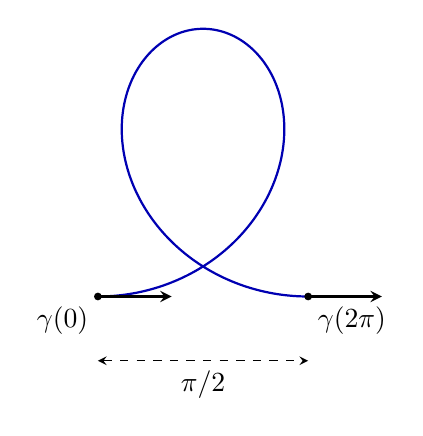
\begin{tikzpicture}[x=1.7cm,y=1.7cm,>=stealth]
	\draw[blue!70!black,thick,domain=0:360,samples=161,smooth,variable=\t] plot ({sin(\t)+0.5*(\t*pi/360+sin(2*\t)/4)},{1-cos(\t)+0.25*sin(\t)^2});
	\fill (0,0) circle (1.4pt) node[below left] {\(\gamma(0)\)};
	\fill ({pi/2},0) circle (1.4pt) node[below right] {\(\gamma(2\pi)\)};
	\draw[->,thick] (0,0)--(0.55,0);
	\draw[->,thick] ({pi/2},0)--({pi/2+0.55},0);
	\draw[<->,dashed] (0,-0.48)--node[below] {\(\pi/2\)} ({pi/2},-0.48);
\end{tikzpicture}

	\caption[切向量接合与位置闭合]{切向量接合与位置闭合。\(\varepsilon=\tfrac12\) 时，曲线转角从 \(0\) 增至 \(2\pi\)，两端的切向量相同，但端点相差 \((\pi/2,0)\)。箭头只表示相应端点的切向方向。}
	\label{g1:fig:closure-displacement}
\end{figure}

正面的例子是 \(k(s)=1/R\)、\(L=2\pi R\)，取初始切向量为 \((1,0)\)，积分得到
\[
	\gamma(s)=\bigl(R\sin(s/R),R(1-\cos(s/R))\bigr).
\]
三项闭合条件都成立，曲线恰为圆。若改用周期 \(4\pi R\)，同一公式仍满足条件，却把圆走了两遍。简单性还要求一个周期内只经过每个点一次。

% !TeX root = ../../Book1.tex
% 纲要标题：### 7.3 平面闭曲线的绕转
% 纲要位置：几何学计划纲要.md，第 383 行。
% 正文状态：初稿；尚未正式审核。

% 纲要内容开始
% 
% * 切向映射的次数
% * 转角定理与简单闭曲线
% * 曲率符号、凸性及反例
% 
% 纲要内容结束

\section{平面闭曲线的绕转}
\label{g1:sec:0703}

沿一条平面闭曲线走一周，位置回到原点，切向量也回到原方向；但连续记录的切向角可能多转了几周。这个整周差把局部的有向曲率同闭曲线的整体形状联系起来。简单性将这个整数限制为 \(1\) 或 \(-1\)，曲率同号则使切向角单调，从而把转角与凸性联系起来。

\subsection{切向映射的次数}
\label{g1:subsec:0703:01}

设 \(\gamma:\mathbb R/L\mathbb Z\rightarrow\mathbb R^2\) 是 \(C^1\) 正则闭曲线；用弧长参数时，\(L\) 是总长，\(T(s)=\gamma'(s)\in S^1\)。闭合在这里包含参数接点的导数相容，因而 \(T(0)=T(L)\)。\cref{g1:lem:circle-angle-lift}说明，给定初始角度后，可以沿区间 \([0,L]\) 唯一地选择连续函数 \(\theta\)，使
\[
	T(s)=(\cos\theta(s),\sin\theta(s)).
\]
前章把圆周角度按整周归一为 \(e^{2\pi iu}\)；本节使用弧度，所以这里的 \(\theta\) 是那里角度提升的 \(2\pi\) 倍。等式 \(T(0)=T(L)\) 只保证 \(\theta(L)-\theta(0)\in2\pi\mathbb Z\)，不要求这个差为零。

\begin{definition}[旋转次数]\label{g1:def:rotation-index}
	设 \(P>0\)，\(\gamma:\mathbb R/P\mathbb Z\to\mathbb R^2\) 为 \(C^1\) 正则闭曲线，令 \(T(t)=\gamma'(t)/\|\gamma'(t)\|\)，并取 \(T\) 在 \([0,P]\) 上的连续角度提升 \(\theta\)。单位切向映射的\term[cishu]{次数}[degree]称为曲线的\term[xuanzhuancishu]{旋转次数}[rotation index]，记为
	\[
		\operatorname{rot}(\gamma)\coloneqq\deg T
		=\frac{\theta(P)-\theta(0)}{2\pi}\in\mathbb Z.
	\]
	若采用弧长参数，则以总长 \(L\) 替代 \(P\)。这里次数就是\cref{g1:thm:circle-fundamental}中圆周映射沿定义域正向一周的绕数；任意两个角度提升相差常数 \(2\pi m\)，故右边不依赖初始角度的选择。
\end{definition}

切向映射在方向圆周上走，原曲线在位置平面上走。旋转次数记录前者，不能与原曲线绕某个指定点的绕数混同：后者需要先选一个不在曲线上的点，而前者不需要这样一个点。

\begin{proposition}[有向曲率的整周积分]\label{g1:prop:total-turning}
	设 \(\gamma:\mathbb R/L\mathbb Z\rightarrow\mathbb R^2\) 是 \(C^2\) 弧长参数正则闭曲线，\(k\) 是按 \(T'=kJT\) 定义的有向曲率，其中 \(J(x,y)=(-y,x)\)。则其连续切向角提升是 \(C^1\) 的，且
	\begin{equation}\label{g1:eq:total-signed-curvature}
		k(s)=\theta'(s),\qquad \int_0^L k(s)\,\mathrm{d}s=2\pi\operatorname{rot}(\gamma).
	\end{equation}
	对一般正则参数 \(t\in[0,P]\)，同一公式写为
	\[
		2\pi\operatorname{rot}(\gamma)
		=\int_0^P\frac{\det(\dot\gamma(t),\ddot\gamma(t))}{|\dot\gamma(t)|^2}\,\mathrm{d}t.
	\]
\end{proposition}
\begin{proof}
	在任一小开弧上，圆周有光滑角度坐标。连续提升在这样的坐标区间内与该局部角度相差固定的 \(2\pi\) 整数倍，所以它具有与 \(T\) 相同的 \(C^1\) 正则性。微分给出
	\[
		T'(s)=\theta'(s)(-\sin\theta(s),\cos\theta(s))=\theta'(s)JT(s).
	\]
	与有向曲率的定义比较得到 \(k=\theta'\)，然后应用微积分基本定理。一般参数下，\cref{g1:prop:arc-length-param}给出 \(\mathrm{d}s=|\dot\gamma|\,\mathrm{d}t\)，而有向曲率公式为 \(k=\det(\dot\gamma,\ddot\gamma)/|\dot\gamma|^3\)；将这两个等式相乘即得最后一式。
\end{proof}

\begin{proposition}[方向与连续变形]\label{g1:prop:rotation-invariance}
	旋转次数在保向正则重参数化和保向平面刚体运动下不变；反向重参数化或平面反射各使它变号。若 \(\gamma_u:\mathbb R/P\mathbb Z\rightarrow\mathbb R^2\) 是一族闭曲线，\((t,u)\mapsto\gamma_u(t)\) 与 \((t,u)\mapsto\partial_t\gamma_u(t)\) 均连续，且后者处处非零，\(u\in[0,1]\)，则 \(\operatorname{rot}(\gamma_u)\) 与 \(u\) 无关。
\end{proposition}
\begin{proof}
	保向重参数化只按原次序走过切向映射；反向重参数化使切向量成为原切向量的负向并逆序走过。取负向只给切向角加上 \(\pi\)，逆序则把总增量变号。保向平面刚体运动给角度加一个常数，反射把角度变为某个常数减去原角度，这证明前两句。

	对连续变形，单位切向量
	\[
		T_u(t)=\frac{\partial_t\gamma_u(t)}{|\partial_t\gamma_u(t)|}
	\]
	构成圆周映射的连续同伦。把平面识别为复平面，考虑 \(T_u(t)/T_u(0)\)，就得到基点始终为 \(1\) 的环路同伦。\cref{g1:thm:circle-fundamental}的同伦不变性使它们的绕数相同，而除以 \(T_u(0)\) 只减去常数角度。
\end{proof}

命题最后一类变形称为\term[zhengzetonglun]{正则同伦}[regular homotopy]：在变形中允许曲线穿过自身，但切向量不能消失。旋转次数因而是正则同伦的不变量。

\subsection{转角定理与简单闭曲线}
\label{g1:subsec:0703:02}

简单闭曲线要求 \(\gamma:\mathbb R/L\mathbb Z\rightarrow\mathbb R^2\) 单射。\cref{g1:thm:jordan-separation}给出其有界内部 \(\Omega\) 和无界外部。在曲线每一点，以切线为横轴，正则性使一小段曲线成为 \(C^1\) 函数的图像；把坐标矩形取得足够小，还能避开其余曲线。图像分出的两侧恰分别属于内部和外部，因为两者的边界都是整条曲线。内部处于行进方向的左侧还是右侧，是随参数局部不变的选择，故在整个参数圆周上一致。称内部位于左侧的行进方向为正向；反转参数即可在两种方向间转换。

\begin{theorem}[转角定理]\label{g1:thm:turning-tangent}
	设 \(\gamma:\mathbb R/L\mathbb Z\rightarrow\mathbb R^2\) 是 \(C^1\) 正则简单闭曲线。正向参数下 \(\operatorname{rot}(\gamma)=1\)，反向参数下 \(\operatorname{rot}(\gamma)=-1\)。特别地，若 \(\gamma\) 为 \(C^2\) 弧长参数曲线，则
	\[
		\int_0^L k(s)\,\mathrm{d}s=
		\begin{cases}
			2\pi,&\text{正向},\\
			-2\pi,&\text{反向}.
		\end{cases}
	\]
\end{theorem}

简单曲线可以有许多凹陷，切向角也可以来回变化。用两个点合拢时的弦方向表示相切方向，就能在参数三角形上统一记录这些变化。\cref{g1:fig:chord-triangle}显示了三条边各自承担的角度变化。

\begin{figure}[htbp]
	\centering
	% !TeX root = ../Book1.tex
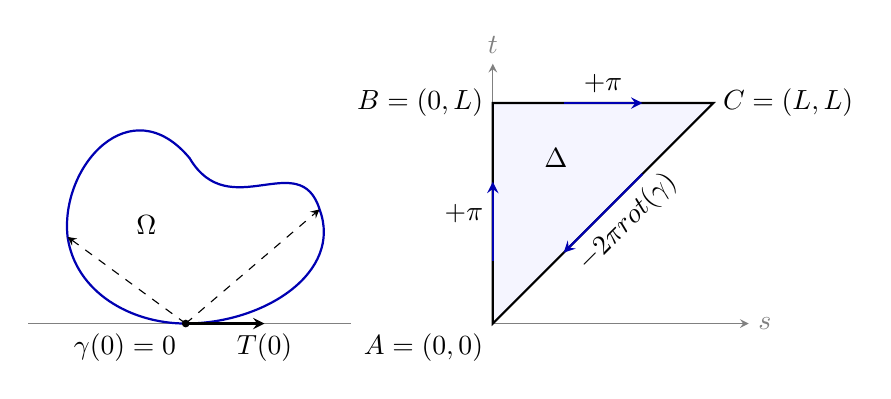
\begin{tikzpicture}[x=1cm,y=1cm,>=stealth]
	\begin{scope}[shift={(1.7,0.25)}]
		\draw[gray] (-2,0)--(2.1,0);
		\draw[thick,blue!70!black] (0,0) .. controls (1,0) and (2,0.65) .. (1.7,1.45) .. controls (1.45,2.25) and (0.55,1.25) .. (0.05,2.1) .. controls (-0.7,3) and (-1.6,2) .. (-1.5,1.1) .. controls (-1.4,0.4) and (-0.7,0) .. (0,0);
		\draw[->,thick] (0,0)--(1,0) node[below] {\(T(0)\)};
		\draw[dashed,->] (0,0)--(1.7,1.45);
		\draw[dashed,->] (0,0)--(-1.5,1.1);
		\fill (0,0) circle (1.4pt);
		\node[below left] at (0,0) {\(\gamma(0)=0\)};
		\node at (-0.5,1.25) {\(\Omega\)};
	\end{scope}
	\begin{scope}[shift={(5.6,0.25)}]
		\fill[blue!4] (0,0)--(0,2.8)--(2.8,2.8)--cycle;
		\draw[->,gray] (0,0)--(3.25,0) node[right] {\(s\)};
		\draw[->,gray] (0,0)--(0,3.3) node[above] {\(t\)};
		\draw[thick] (0,0)--(0,2.8)--(2.8,2.8)--cycle;
		\draw[->,blue!70!black,thick] (0,0.8)--(0,1.8);
		\draw[->,blue!70!black,thick] (0.9,2.8)--(1.9,2.8);
		\draw[->,blue!70!black,thick] (1.9,1.9)--(0.9,0.9);
		\node[left] at (0,1.4) {\(+\pi\)};
		\node[above] at (1.4,2.8) {\(+\pi\)};
		\node[rotate=45,below] at (1.5,1.5) {\(-2\pi\operatorname{rot}(\gamma)\)};
		\node at (0.8,2.1) {\(\Delta\)};
		\node[below left] at (0,0) {\(A=(0,0)\)};
		\node[left] at (0,2.8) {\(B=(0,L)\)};
		\node[right] at (2.8,2.8) {\(C=(L,L)\)};
	\end{scope}
\end{tikzpicture}

	\caption[弦方向的参数三角形]{左图以曲线最低点为基点，此点发出的所有弦均指向闭上半平面。右图的两条直角边分别记录基点弦方向及其负向，各有角增量 \(\pi\)；斜边逆向记录切向映射。图中曲线仅为示意，证明不要求凸性。}
	\label{g1:fig:chord-triangle}
\end{figure}

\begin{proof}
	先取弧长参数；\(C^1\) 正则性足以使用\cref{g1:prop:arc-length-param}，旋转次数不因这种保向重参数化而改变。旋转、平移平面并移动参数起点，使 \(\gamma(0)=\gamma(L)=0\) 是曲线第二坐标的最小点，整条曲线位于 \(y\geq0\)。该点的切向量水平。正向时 \(T(0)=(1,0)\)：最低点下方属于无界外部，局部内部在切线的上侧，正向要求它位于左方。

	在闭三角形
	\[
		\Delta=\{(s,t):0\leq s\leq t\leq L\}
	\]
	上定义一个圆周值映射。对 \(s<t\)、\((s,t)\ne(0,L)\)，令
	\[
		F(s,t)=\frac{\gamma(t)-\gamma(s)}{|\gamma(t)-\gamma(s)|}.
	\]
	简单性保证分母不为零。在对角线上令 \(F(s,s)=T(s)\)，在余下角点令 \(F(0,L)=-T(0)\)。这些赋值确实连续。对角线附近，
	\[
		\frac{\gamma(t)-\gamma(s)}{t-s}
		=\frac1{t-s}\int_s^t T(v)\,\mathrm{d}v
	\]
	一致趋近相应的单位切向量；这是紧区间上 \(T\) 一致连续的直接结果。在角点 \((0,L)\) 附近，设 \(a=s\)、\(b=L-t\)，由两端相容的导数 \(T(0)=T(L)\)，
	\[
		\gamma(L-b)-\gamma(a)=-(a+b)T(0)+o(a+b).
	\]
	归一化后恰趋向 \(-T(0)\)，也包括 \(a=0\) 或 \(b=0\) 的情形。

	令 \(A=(0,0)\)、\(B=(0,L)\)、\(C=(L,L)\)。沿 \(A\to B\) 走，\(F(0,t)\) 是从原点发出的弦方向，始终在闭上半圆。因此其连续角度可直接取为 \([0,\pi]\) 中的值，从 \(0\) 变到 \(\pi\)，总增量为 \(\pi\)。沿 \(B\to C\) 走，
	\[
		F(s,L)=-F(0,s),
	\]
	故在前一角度上加 \(\pi\)，得到从 \(\pi\) 到 \(2\pi\) 的提升，总增量仍为 \(\pi\)。沿 \(C\to A\) 的对角线走，方向映射为逆向的 \(T\)，总增量是 \(-2\pi\operatorname{rot}(\gamma)\)。

	另一方面，边界环路 \(F|_{\partial\Delta}\) 的总增量必须为零。具体地，把三角形边界上的点 \(x\) 沿 \((1-u)x+uA\) 缩到 \(A\)，再复合 \(F\)，就得到固定基点 \(F(A)\) 的零伦；\cref{g1:thm:circle-fundamental}说明它的绕数为零。三段角度相接，因而
	\[
		0=\pi+\pi-2\pi\operatorname{rot}(\gamma).
	\]
	这给出正向的结论。反向时旋转次数变号；\(C^2\) 情形的曲率积分再由\eqref{g1:eq:total-signed-curvature}得到。
\end{proof}

简单性在证明中有明确的用途：它保证任意两个不同参数点之间的弦方向都有定义。自交点会在三角形内部产生未定义点，边界映射就未必能延拓到整个三角形，绕数为零的论证也随之失效。

\subsection{曲率符号、凸性及反例}
\label{g1:subsec:0703:03}

若 \(k\geq0\)，切向角不减；再要求它只转一周，就能同时控制绕行次数并判断曲线的凸性。若一条简单闭曲线的像是某个有非空内部的紧凸集的边界，就称它为\term[tuquxian]{凸曲线}[convex curve]；这里允许边界包含线段。

\begin{theorem}[曲率符号与凸性]\label{g1:thm:curvature-convexity}
	设 \(L>0\)，\(\gamma:\mathbb R/L\mathbb Z\rightarrow\mathbb R^2\) 是 \(C^2\) 弧长参数正则闭曲线，平面取标准定向，以 \(k\) 记沿参数递增方向的有向曲率。
	\begin{enumerate}
		\item 若 \(k\geq0\) 且 \(\operatorname{rot}(\gamma)=1\)，则 \(\gamma\) 自动为简单闭曲线，且按正向恰好描出一个紧凸集的边界一周。
		\item 若已知 \(\gamma\) 是正向简单闭曲线，则它为凸曲线，当且仅当 \(k\geq0\)。
	\end{enumerate}
	相应地，反向时把 \(k\geq0\)、旋转次数 \(1\) 改为 \(k\leq0\)、旋转次数 \(-1\)。
\end{theorem}
\begin{proof}
	先假设 \(k\geq0\)、旋转次数为 \(1\)。切向角提升满足 \(\theta'=k\geq0\)、\(\theta(s+L)=\theta(s)+2\pi\)。任意选一个起点，平移和旋转后可设它的参数为 \(0\)、位置为 \(0\)、切向角为 \(0\)。记 \(\gamma(s)=(x(s),y(s))\)，则
	\[
		y'(s)=\sin\theta(s),\qquad 0\leq\theta(s)\leq2\pi,\qquad y(0)=y(L)=0.
	\]
	在切向角从 \(0\) 增至 \(\pi\) 的阶段，\(y\) 不减；从 \(\pi\) 增至 \(2\pi\) 的阶段，\(y\) 不增。因此 \(y(s)\geq0\)：整条曲线在所选起点的有向切线左侧。

	还须排除中途回到起点，不能仅由半平面包含关系断言简单性。若 \(0<\theta(s)\leq\pi\)，连续角度在此前经过 \((0,\pi)\) 中的一段，故 \(y(s)=\int_0^s\sin\theta(v)\,\mathrm{d}v>0\)。若 \(\pi\leq\theta(s)<2\pi\)，则
	\[
		y(s)=-\int_s^L\sin\theta(v)\,\mathrm{d}v>0.
	\]
	余下的 \(\theta(s)=0\) 情形，由单调性知 \([0,s]\) 上 \(T=(1,0)\)，所以 \(\gamma(s)=(s,0)\ne0\)；\(\theta(s)=2\pi\) 时，同理 \(\gamma(s)=(-(L-s),0)\ne0\)，这里均取 \(0<s<L\)。起点任意，所以两个不同参数类不可能具有同一像点，\(\gamma\) 为简单闭曲线。

	设其有界内部为 \(\Omega\)，\(K=\overline\Omega\)。转角定理表明当前参数为正向，故局部内部在左侧。前两段已经证明每一点的闭左半平面
	\[
		H_s=\{p:\langle p-\gamma(s),JT(s)\rangle\geq0\}
	\]
	包含整条曲线，也包含 \(K\)。后一断言可这样看：线性函数 \(\langle p-\gamma(s),JT(s)\rangle\) 在紧集 \(K\) 上取到最小值，若它为负且不在边界取到，就会在开集 \(\Omega\) 内有局部最小值，这与其非零线性梯度矛盾。

	事实上 \(K=\bigcap_sH_s\)。为证反向包含，取 \(p\notin K\)，在 \(K\) 中取距离 \(p\) 最近的点 \(q\)。最近点必在边界上，写 \(q=\gamma(s)\)；对 \(|p-\gamma(v)|^2\) 求导可知 \(p-q\perp T(s)\)。线段 \((q,p]\) 不碰 \(K\)，否则有更近的点。若 \(p-q\) 是左法向，线段靠近 \(q\) 的一小段就位于局部内部，与此矛盾。因此 \(p-q\) 是右法向，\(p\notin H_s\)。所求等式成立，而闭半平面的交是凸集。这证明第1项。

	现在假设曲线已简单并取正向。若 \(k\geq0\)，转角定理给出旋转次数 \(1\)，第1项适用。反之，设 \(K=\overline\Omega\) 凸。先说明每条切线都是支撑线。把任一边界点移到原点，使正向切向量为 \((1,0)\)，则附近边界写成 \(y=f(x)\)，其中 \(f(0)=f'(0)=0\)，局部 \(K\) 位于图像上方。如果某个 \(p=(p_x,p_y)\in K\) 满足 \(p_y<0\)，凸性使 \(tp\in K\) 对 \(0<t<1\) 成立。但 \(f(tp_x)=o(t)\)，故充分小时 \(tp_y<f(tp_x)\)，矛盾。因此 \(K\) 在切线的闭上半平面内，特别地 \(f(x)\geq0\)。于是 \(f''(0)\geq0\)。在这一坐标和方向下有向曲率为 \(f''(0)/(1+f'(0)^2)^{3/2}\)，所以 \(k\geq0\)。边界点任意，第2项得证。
\end{proof}

在证明中，允许 \(k=0\) 至关重要：它使 \(\theta\) 可以保持不变，对应曲线中的直线段。若正向简单闭曲线处处 \(k>0\)，则每条支撑切线只接触曲线一个点。事实上，对固定起点，切向角严格增加，证明中的法向高度在其余参数处都严格为正。因此此时所围凸集严格凸，即边界不包含非退化线段。逆命题却不成立：严格凸边界的个别点仍可以曲率为零，章末的四次曲线给出例子。

\begin{example}[正曲率仍可能重复绕行]\label{g1:exm:multiple-circle-turning}
	对整数 \(m\geq2\)，考虑 \(\gamma(t)=(\cos mt,\sin mt)\)，\(t\in\mathbb R/2\pi\mathbb Z\)。它正则，速率为 \(m\)，有向曲率恒为 \(1\)，但同一圆周被走了 \(m\) 遍。其总长为 \(2\pi m\)，旋转次数为 \(m\)。所以在尚未知道简单性时，不能把 \(k>0\) 直接当作简单凸曲线的判据。
\end{example}

\begin{example}[旋转一次仍可能有自交]\label{g1:exm:rotation-one-self-intersection}
	令
	\[
		\gamma(t)=(\cos t,\sin t+2\sin3t),\qquad t\in\mathbb R/2\pi\mathbb Z.
	\]
	当 \(\sin t\ne0\) 时，第一坐标导数 \(-\sin t\) 非零；在 \(t=0,\pi\) 处，第二坐标导数分别为 \(7,-7\)，故曲线处处正则。对 \(0<t<\pi\)，切向量的第一坐标为负，其角度可以连续取在 \((\pi/2,3\pi/2)\)，并从 \(\pi/2\) 走到 \(3\pi/2\)；对 \(\pi<t<2\pi\)，第一坐标为正，角度继续从 \(3\pi/2\) 走到 \(5\pi/2\)。两段合计增量 \(2\pi\)，所以旋转次数为 \(1\)。

	然而
	\[
		\sin t+2\sin3t=\sin t\,(8\cos^2t-1).
	\]
	选 \(t_0\in(0,\pi/2)\) 满足 \(\cos t_0=1/\sqrt8\)，就有 \(\gamma(t_0)=\gamma(2\pi-t_0)\)，因而曲线不简单。它的曲率也不是同号：\(\det(\dot\gamma,\ddot\gamma)\) 在 \(t=0\) 为 \(7\)，在 \(t=\pi/2\) 为 \(-17\)。这个例子把凸性判据的两个条件分开了：整周数为 \(1\) 只控制净转角，曲率符号才控制转向是否来回反复。
\end{example}

本节积分的是有向曲率，左转和右转会抵消。下一节改看 \(\int|k|\,\mathrm{d}s\) 及其空间曲线版本：即使净转角很小，实际弯曲的总量仍可能很大。
% 纲要条目排为编号小节标题，并进入目录与书签；说明段仍保留于纲要注释中。

% !TeX root = ../../Book1.tex
% 纲要标题：### 7.4 总曲率与空间曲线
% 纲要位置：几何学计划纲要.md，第 389 行。
% 正文状态：初稿；尚未正式审核。

% 纲要内容开始
% 
% * 球面切向曲线和总曲率
% * Fenchel 不等式的几何证明
% * 等号条件与平面凸曲线
% * 结型施加的进一步限制：准确陈述，不将结理论预设为先修
% 
% ---
% 
% 纲要内容结束

\section{总曲率与空间曲线}
\label{g1:sec:0704}

平面简单闭曲线的切向量一共转过一周，但空间曲线没有一个固定平面供我们比较转角的正负。仍然可以把每个单位切向量的起点移到原点，观察它的终点在单位球面上走了多远。闭合条件将迫使这条球面曲线有足够的长度；当长度恰好达到最小值时，空间曲线反而必须落回一个平面。这个论证只需要单位切向量，不要求处处有 Frenet 法向量，因而也能处理零曲率点。

\subsection{球面切向曲线和总曲率}
\label{g1:subsec:0704:01}

\begin{definition}[总曲率与切向示性曲线]\label{g1:def:total-curvature}
	设 \(\gamma:[0,L]\to\mathbb R^3\) 是 \(C^2\) 单位速率曲线，其中 \(L>0\)，允许曲线不闭合。其单位切向量 \(T(s)=\gamma'(s)\) 给出一条 \(C^1\) 球面曲线
	\[
		T:[0,L]\longrightarrow S^2,\qquad
		S^2=\{x\in\mathbb R^3:\|x\|=1\},
	\]
	称为\term[qiexiangshixingquxian]{切向示性曲线}[tangent indicatrix]。定义 \(\gamma\) 的\term[zongqulv]{总曲率}[total curvature]为
	\begin{equation}\label{g1:eq:total-curvature}
		\operatorname{TC}(\gamma)\coloneqq\int_0^L\kappa(s)\,\mathrm{d}s
		=\int_0^L\|T'(s)\|\,\mathrm{d}s.
	\end{equation}
	\symidx{\(\operatorname{TC}(\gamma)\)：曲线的总曲率}
	对于任意紧参数区间上的 \(C^2\) 正则曲线，先按\cref{g1:prop:arc-length-param}换成弧长参数，或等价地在原参数 \(t\) 下使用 \(\int\kappa(t)\|\dot\gamma(t)\|\,\mathrm{d}t\)。
\end{definition}

右端正是切向示性曲线的长度，计入重复经过同一球面弧的次数。它并不是集合 \(T([0,L])\) 的“去重后长度”。原曲线的一段直线使 \(T\) 停在一点，不给总曲率增加长度；原曲线绕同一圆走两遍，则切向示性曲线也走两遍。由于 \(\kappa=\|T'\|\ge0\)，总曲率没有正负抵消。平面有向曲率 \(k\) 与这里的量满足 \(\kappa=|k|\)，因此 \(\int k\,\mathrm{d}s\) 和 \(\operatorname{TC}(\gamma)\) 应当区分。

\begin{example}[尺度与重复参数]\label{g1:exm:total-curvature-circle}
	半径为 \(R>0\) 的圆走一周时，\(\kappa=1/R\)，长度为 \(2\pi R\)，故总曲率是 \(2\pi\)。更一般地，对任意 \(a>0\)，伸缩后的曲线 \(a\gamma\) 的弧长元变成 \(a\,\mathrm{d}s\)，曲率变成 \(\kappa/a\)，所以总曲率不变。若 \(\gamma_m(t)=(R\cos mt,R\sin mt,0)\)，其中 \(m\) 是非零整数且 \(0\le t\le2\pi\)，则总曲率为 \(2\pi|m|\)。同一个圆形像集并未确定总曲率；走过它的次数仍然是参数曲线的一部分。
\end{example}

闭曲线还满足一个比 \(T(0)=T(L)\) 更有用的约束：
\begin{equation}\label{g1:eq:tangent-balance}
	\int_0^L T(s)\,\mathrm{d}s=\gamma(L)-\gamma(0)=0.
\end{equation}
它表示各方向的位移必须抵消。例如，若存在非零向量 \(a\)，使 \(a\cdot T(s)>0\) 对所有 \(s\) 成立，那么整条曲线始终向 \(a\) 方向前进，不可能闭合。稍后还需要边界情形：若 \(a\cdot T(s)\ge0\) 处处成立，则连续性和\eqref{g1:eq:tangent-balance}迫使 \(a\cdot T(s)=0\) 处处成立，此时 \(\gamma\) 落在一个垂直于 \(a\) 的平面内。

\subsection{Fenchel 不等式的几何证明}
\label{g1:subsec:0704:02}

我们把球面上两点 \(p,q\) 的夹角记为 \(d_S(p,q)=\arccos(p\cdot q)\in[0,\pi]\)。下面证明，在球面上绕行不能比这段角距离更短。这也是下一小节判断等号的工具。

\begin{lemma}[球面弧长与端点夹角]\label{g1:lem:spherical-arc-distance}
	设 \(c:[a,b]\to S^2\) 是 \(C^1\) 曲线，允许 \(c'\) 为零。则
	\[
		d_S(c(a),c(b))\le\int_a^b\|c'(t)\|\,\mathrm{d}t.
	\]
	若 \(c(a)=p\)、\(c(b)=-p\)，且右端等于 \(\pi\)，则存在一个与 \(p\) 垂直的单位向量 \(v\)，使
	\[
		c(t)=p\cos u(t)+v\sin u(t),\qquad
		u(t)=\int_a^t\|c'(r)\|\,\mathrm{d}r.
	\]
	因而该弧沿一条半大圆单调前进，可以停顿，但不能折返。
\end{lemma}

\begin{proof}
	记 \(p=c(a)\)。由于 \(c\cdot c'=0\)，将 \(p\) 分解到 \(c(t)\) 方向及其垂直平面，得到
	\[
		|p\cdot c'(t)|\le\sqrt{1-(p\cdot c(t))^2}\,\|c'(t)\|.
	\]
	直接对 \(\arccos(p\cdot c)\) 求导会在 \(c=\pm p\) 处遇到分母为零。为保留这些端点，先取 \(0<\varepsilon<1\)，令
	\[
		\theta_\varepsilon(t)=\arccos\bigl((1-\varepsilon)p\cdot c(t)\bigr).
	\]
	此时分母严格为正，而且
	\[
		|\theta_\varepsilon'(t)|
		\le
		\frac{(1-\varepsilon)\sqrt{1-(p\cdot c(t))^2}}
		{\sqrt{1-(1-\varepsilon)^2(p\cdot c(t))^2}}\,
		\|c'(t)\|
		\le\|c'(t)\|.
	\]
	积分并令 \(\varepsilon\to0\)，便得端点夹角的估计。相同论证适用于曲线的任意子区间。

	现在设端点为 \(p,-p\)，总长恰为 \(\pi\)。令 \(\theta(t)=\arccos(p\cdot c(t))\)。分别从两端使用刚证的估计，得到
	\[
		\theta(t)\le u(t),\qquad
		\pi-\theta(t)\le\pi-u(t),
	\]
	所以 \(\theta(t)=u(t)\)。在 \(0<u(t)<\pi\) 的区间上，定义
	\[
		v(t)=\frac{c(t)-p\cos u(t)}{\sin u(t)}.
	\]
	它是 \(C^1\) 单位向量，且 \(v(t)\perp p\)。微分上式所给的 \(c=p\cos u+v\sin u\)，利用 \(v'\perp p,v\)，可得
	\[
		\|c'\|^2=(u')^2+\sin^2u\,\|v'\|^2.
	\]
	定义给出 \(u'=\|c'\|\)，故 \(v'=0\)。因为 \(u\) 单调，\(0<u<\pi\) 的原像是一个区间，因而这里的 \(v\) 是同一个常向量。剩余端段上 \(u=0\) 或 \(u=\pi\)，对应 \(c=p\) 或 \(c=-p\)，公式仍然成立。
\end{proof}

\begin{lemma}[短球面闭曲线的半球约束]\label{g1:lem:short-spherical-loop}
	设 \(c\) 是一条 \(C^1\) 球面闭曲线，将它按经过顺序分成长度相等的两段，分点为 \(p,q\)。若总长度小于 \(2\pi\)，则
	\[
		(p+q)\cdot c(t)>0\qquad\text{对所有 }t.
	\]
	若总长度等于 \(2\pi\) 且 \(q\ne-p\)，则上式改为非负不等式，并且在分点 \(p\) 处严格为正。
\end{lemma}

\begin{proof}
	累计长度是连续函数，所以可以取到半长分点；长度为零时任取分点即可。任一点 \(x=c(t)\) 位于两段之一。从该段的两端走到 \(x\)，由\cref{g1:lem:spherical-arc-distance}有
	\[
		\alpha+\beta\le\frac{\operatorname{length}(c)}2,\qquad
		\alpha=d_S(p,x),\quad\beta=d_S(q,x).
	\]
	而
	\[
		(p+q)\cdot x=\cos\alpha+\cos\beta
		=2\cos\frac{\alpha+\beta}{2}\cos\frac{\alpha-\beta}{2}.
	\]
	若总长小于 \(2\pi\)，则 \(\alpha+\beta<\pi\)，两个余弦都严格为正。若总长等于 \(2\pi\)，则两者都非负；在 \(x=p\) 处，该内积为 \(1+p\cdot q>0\)，最后一个严格不等式正用了 \(q\ne-p\)。
\end{proof}

这个引理把“转得太少”变成了“所有方向都偏向同一侧”。其中 \(p+q\) 指向夹角的中间方向；两段都不足半个大圆时，它们就不能绕到这个方向的背后。

\begin{theorem}[Fenchel 不等式]\label{g1:thm:fenchel}
	设 \(\gamma:\mathbb R/L\mathbb Z\to\mathbb R^3\) 是 \(C^2\) 正则闭曲线，按弧长参数化，\(L>0\)。则
	\[
		\operatorname{TC}(\gamma)=\int_0^L\kappa(s)\,\mathrm{d}s\ge2\pi.
	\]
	这里不假设 \(\gamma\) 简单，也不假设 \(\kappa>0\)。
\end{theorem}

\begin{proof}
	若总曲率小于 \(2\pi\)，切向示性曲线 \(T\) 的长度也小于 \(2\pi\)。对它应用\cref{g1:lem:short-spherical-loop}，取得两个半长分点 \(p,q\)，使 \((p+q)\cdot T(s)>0\) 处处成立。于是
	\[
		(p+q)\cdot\int_0^L T(s)\,\mathrm{d}s>0,
	\]
	这与闭合约束\eqref{g1:eq:tangent-balance}矛盾。
\end{proof}

这一结论通常称为\term[fenchelbudengshi]{Fenchel 不等式}[Fenchel's inequality]，包括等号条件的整体陈述也称为 Fenchel 定理。\footnote{Fenchel，芬切尔，Werner Fenchel（1905--1988），生于德国、后在丹麦工作的数学家，研究凸性理论及非欧几何中的离散群。}原曲线即使在空间里不断改变弯曲平面，也不能把闭合所需的总转向减少到一周以下。文献中的另一种证明从内接多边形的外角和出发，见\cite[Theorem 3.4]{Milnor1950}；这里的球面证明则使零曲率段的作用直接可见。

\subsection{等号条件与平面凸曲线}
\label{g1:subsec:0704:03}

不等式的证明很短，但等号还要回答三个不同的问题：切向量是否在固定平面内，它沿这个平面的单位圆是否折返，以及原曲线是否可能重叠或自交。以下论证依次排除这些可能。

\begin{theorem}[Fenchel 不等式的等号条件]\label{g1:thm:fenchel-equality}
	设 \(\gamma:\mathbb R/L\mathbb Z\to\mathbb R^3\) 是 \(C^2\) 单位速率闭曲线，\(L>0\)。则 \(\operatorname{TC}(\gamma)=2\pi\) 当且仅当 \(\gamma\) 简单，其像是某个仿射平面内具有非空内部的紧凸集的边界，并且参数将该边界走一周。允许曲率在点或区间上为零。
\end{theorem}

\begin{proof}
	先设总曲率为 \(2\pi\)，记累计曲率
	\[
		u(s)=\int_0^s\kappa(r)\,\mathrm{d}r,\qquad 0\le s\le L.
	\]
	把 \(u\) 延拓为满足 \(u(s+L)=u(s)+2\pi\) 的函数。任取 \(s<t\le s+L\)，使 \(u(t)-u(s)=\pi\)。这两个时刻把切向示性曲线分成长度均为 \(\pi\) 的两段。令 \(p=T(s)\)、\(q=T(t)\)。如果 \(q\ne-p\)，\cref{g1:lem:short-spherical-loop}给出
	\[
		(p+q)\cdot T(r)\ge0\quad\text{处处成立},
		\qquad (p+q)\cdot T(s)>0.
	\]
	连续性使严格正值保持在一个参数小区间上，因此其积分严格为正，仍与\eqref{g1:eq:tangent-balance}矛盾。所以任何这样的一对半长分点都互为对径点。

	取 \(p=T(0)\)，并取 \(s_1,s_2,s_3\)，使 \(u(s_j)=j\pi/2\)。第一半段从 \(p\) 到 \(-p\)，长度为 \(\pi\)，故\cref{g1:lem:spherical-arc-distance}给出一个单位向量 \(v\perp p\)，使
	\[
		T(s)=p\cos u(s)+v\sin u(s)\qquad(0\le s\le s_2).
	\]
	特别地 \(T(s_1)=v\)。第二半段也必须沿某条半大圆前进，可以写成
	\[
		T(s)=-p\cos(u(s)-\pi)+w\sin(u(s)-\pi)\qquad(s_2\le s\le L),
	\]
	其中 \(w\perp p\) 是单位向量。由于 \(s_1,s_3\) 又是一对半长分点，\(w=T(s_3)=-T(s_1)=-v\)。因此两段实际合成同一个大圆，而且
	\begin{equation}\label{g1:eq:fenchel-equality-tangent}
		T(s)=p\cos u(s)+v\sin u(s)\qquad(0\le s\le L).
	\end{equation}

	积分表明 \(\gamma(s)-\gamma(0)\) 始终属于平面 \(\operatorname{span}\{p,v\}\)。在以 \(p,v\) 为正向正交基的这个平面里，\(u(s)\) 正是一个连续切角；它单调不减，总增量为 \(2\pi\)。\cref{g1:thm:curvature-convexity}的充分性方向适用于闭正则曲线，并不预设简单性：切角单调增加一周时，所有切线都是同侧支撑线，而且曲线没有重复点。因此 \(\gamma\) 简单，并且沿一个紧凸集的边界走一周。

	反过来，设 \(\gamma\) 简单且是平面紧凸集的边界。选择使凸集位于左侧的方向，由\cref{g1:thm:curvature-convexity}，其有向曲率 \(k\ge0\)；由\cref{g1:thm:turning-tangent}，\(\int_0^L k\,\mathrm{d}s=2\pi\)。于是 \(\operatorname{TC}(\gamma)=\int_0^L|k|\,\mathrm{d}s=2\pi\)。反向行走时 \(k\) 改变符号，总曲率不变。
\end{proof}

% !TeX root = ../Book1.tex
\begin{figure}[htbp]
	\centering
	\begin{tikzpicture}[scale=1,>=stealth,line cap=round,line join=round]
		\begin{scope}[xshift=-3cm]
			\draw[thick] (0,0) ellipse (1.6 and 1.05);
			\draw[->,blue!70!black,thick] (1.6,0) -- (1.6,0.72) node[right] {\(p\)};
			\draw[->,blue!70!black,thick] (0,1.05) -- (-0.72,1.05) node[above] {\(v\)};
			\draw[->,blue!70!black,thick] (-1.6,0) -- (-1.6,-0.72) node[left] {\(-p\)};
			\draw[->,blue!70!black,thick] (0,-1.05) -- (0.72,-1.05) node[below] {\(-v\)};
			\node at (0,-1.85) {平面凸曲线};
		\end{scope}
		\draw[->,thick] (-0.75,0) -- (0.75,0) node[midway,above] {\(T\)};
		\begin{scope}[xshift=3cm]
			\draw[thick,blue!70!black] (0,0) circle (1.15);
			\draw[->,thick,blue!70!black] (80:1.15) arc (80:120:1.15);
			\draw[->,thick,blue!70!black] (260:1.15) arc (260:300:1.15);
			\fill (0,1.15) circle (1.5pt) node[above] {\(p\), \(u=0,2\pi\)};
			\fill (-1.15,0) circle (1.5pt) node[left] {\(v\)};
			\fill (0,-1.15) circle (1.5pt) node[below] {\(-p\), \(u=\pi\)};
			\fill (1.15,0) circle (1.5pt) node[right] {\(-v\)};
			\node at (0,-1.85) {球面中的一个大圆};
		\end{scope}
	\end{tikzpicture}
	\caption{等号情形中，切向示性曲线按累计曲率 \(u\) 沿大圆前进一周。这里以椭圆示意原曲线；一般凸曲线若有直线段，切向量会在相应方向停顿。}
	\label{g1:fig:total-curvature}
\end{figure}


证明中的 \(u\) 是累计曲率，未必是合法的正则重参数：在直线段上 \(u'=0\)，甚至可能一段时间不变化。我们只把它代入\eqref{g1:eq:fenchel-equality-tangent}，没有除以 \(\kappa\)，也没有要求 \(u\) 可逆。\cref{g1:fig:total-curvature}所画的圆周运动可以在个别方向上停顿；因此等号条件是“平面凸曲线”，不是“圆”，也不是“处处严格正曲率的平面曲线”。

\begin{corollary}[非平面性的严格代价]\label{g1:cor:nonplanar-total-curvature}
	任何像不包含在一个仿射平面内的 \(C^2\) 正则闭空间曲线，都有 \(\operatorname{TC}(\gamma)>2\pi\)。任何自交的 \(C^2\) 正则闭空间曲线也有同样的严格不等式。
\end{corollary}

\begin{proof}
	\cref{g1:thm:fenchel}给出非严格下界，而\cref{g1:thm:fenchel-equality}排除了这两种情形中的等号。
\end{proof}

\subsection{结型施加的进一步限制：准确陈述，不将结理论预设为先修}
\label{g1:subsec:0704:04}

非平面性取决于当前摆放方式。一个平面圆被轻微拉出平面后，总曲率已经严格大于 \(2\pi\)，但仍然可以完整地拉回原来的圆，不必让曲线穿过自身。结型问的是后一类变形能否做到，其限制比“目前不在平面内”更强。

\begin{definition}[结与平凡结]\label{g1:def:knot-unknot}
	本小节的\term[jie]{结}[knot]指 \(\mathbb R^3\) 中 \(C^2\) 正则嵌入圆周的像。两个结 \(K_0,K_1\) 具有相同\term[jiexing]{结型}[knot type]，是指存在 \(\mathbb R^3\) 的环境同痕 \(H_t\)，使 \(H_1(K_0)=K_1\)。这里沿用\cref{g1:def:ambient-isotopy}的定义：\(H_0=\mathrm{id}\)，且 \((x,t)\mapsto(H_t(x),t)\) 是 \(\mathbb R^3\times[0,1]\) 的同胚。与平面圆有相同结型的结称为\term[pingfanjie]{平凡结}[unknot]，否则称为非平凡结。
\end{definition}

环境同痕移动的是整个周围空间，每一时刻都保持可逆，因而曲线上不同的点不能在变形途中穿过彼此。一般的道路同伦没有这个限制；在 \(\mathbb R^3\) 中任意闭路都可以连续收缩，并不能据此说所有结都平凡。结型只保留嵌入的拓扑性质，不要求变形保持长度或曲率。

\begin{theorem}[Fáry--Milnor 定理]\label{g1:thm:fary-milnor}
	设 \(\gamma:S^1\to\mathbb R^3\) 是 \(C^2\) 正则嵌入，且它的像是非平凡结。则
	\[
		\operatorname{TC}(\gamma)>4\pi.
	\]
	等价地，若一个 \(C^2\) 正则嵌入圆周的总曲率不超过 \(4\pi\)，它必为平凡结。
\end{theorem}

这就是\term[farymilnordingli]{Fáry--Milnor 定理}[Fáry--Milnor theorem]。\footnote{Fáry，法里，匈牙利姓名为 Fáry István（1922--1984），匈牙利出生的数学家，研究几何与代数拓扑，证明了平面图的直线嵌入定理。Milnor，米尔诺，John Willard Milnor（1931年生），美国数学家，在微分拓扑、代数 \(K\) 理论和动力系统中有重要工作。}本章引用这一结论，不展开证明。所用光滑版本可由\cite[Theorem 2.2; Corollary 4.6]{Milnor1950}直接得到：前一处将原文以多边形定义的总曲率与这里的积分相等同，后一处给出严格的 \(4\pi\) 下界。其证明还需要把有限总曲率的结在环境同痕下替换为适当的内接多边形，并研究各投影方向的高度极值数；这些结论在该文的 Sections 3--4 中建立。

\begin{example}[很大的总曲率并不保证打结]\label{g1:exm:unknot-large-curvature}
	考虑平面极坐标曲线
	\[
		\gamma(t)=r(t)(\cos t,\sin t,0),\qquad
		r(t)=1+\tfrac12\cos4t,\qquad 0\le t\le2\pi.
	\]
	因为 \(r\ge1/2\)，每个极角只有一个点，而且 \(\|\dot\gamma(t)\|^2=r'(t)^2+r(t)^2>0\)，所以这是 \(C^\infty\) 正则简单闭曲线。它是平凡结：在柱坐标 \((\rho,\phi,z)\) 中，
	\[
		H_a(\rho,\phi,z)=
		\left(\frac{\rho}{1+(a/2)\cos4\phi},\phi,z\right),
		\qquad 0\le a\le1,
	\]
	给出把它移到单位圆的环境同痕。轴上令 \(H_a(0,0,z)=(0,0,z)\)；分母一致介于 \(1/2\) 与 \(3/2\) 之间，因此映射及逆映射在轴上也连续。

	它的总曲率却大于 \(4\pi\)。把平面视为复平面，有 \(\dot\gamma(t)=e^{it}(r'(t)+ir(t))\)，所以可取切角
	\[
		\theta(t)=t+\frac\pi2-\arctan\frac{r'(t)}{r(t)}.
	\]
	在 \(t_j=(2j+1)\pi/8\) 处，\(r=1\)、\(r'=-2(-1)^j\)，故
	\[
		\theta(t_j)=t_j+\frac\pi2+(-1)^j A,\qquad A=\arctan2.
	\]
	把 \(j=0,\ldots,8\) 的相邻切角差取绝对值并求和，八项按奇偶配成四对，每对为 \(4A\)。由于总变差至少等于任何分割上的变差和，
	\[
		\operatorname{TC}(\gamma)=\int_{t_0}^{t_0+2\pi}|\theta'(t)|\,\mathrm{d}t
		\ge16\arctan2>4\pi.
	\]
	所以 Fáry--Milnor 定理给出的是非平凡结的必要曲率代价，不能反过来凭一个大总曲率数值断定曲线打结。
\end{example}
% 纲要条目排为编号小节标题，并进入目录与书签；说明段仍保留于纲要注释中。


\begin{chaptersummary}
	弧长把行走速度从几何数据中消去。平面有向曲率 \(k\) 是切向角的导数，空间非负曲率 \(\kappa\) 是单位切向量的变化率；在 \(\kappa>0\) 时，挠率与 Frenet 方程继续记录密切平面的转动。零曲率不等于曲线失去正则性，平行法标架可以在这样的点继续，而 Frenet 主法向一般不能连续延拓。

	\ProseParagraphBreak

	斜对称的标架方程保持正交性，积分其切向量便恢复曲线。给定同一弧长参数下的正曲率与挠率，曲线在保向刚性运动意义下唯一；平面则使用允许变号或为零的有向曲率。空间反射使挠率变号，参数反向不使挠率变号。周期数据只保证重复的刚性关系，真正闭合还要求标架和总位移同时相合。

	\ProseParagraphBreak

	平面闭曲线的有向曲率积分等于 \(2\pi\) 倍的旋转次数。简单性使全部弦方向能在参数三角形上连续组织起来，从而迫使转角为正或负一周。对正向简单闭曲线，曲率非负恰好刻画凸性；在尚未知道简单性时，非负曲率还需与旋转次数为 \(1\) 合用。严格凸允许个别零曲率点，正曲率也不能排除多次绕行。

	\ProseParagraphBreak

	总曲率计算切向量在单位球面上走过的总长度，没有有向转角的正负抵消。闭合使所有切向量的弧长平均为零，由此得到 Fenchel 不等式 \(\int\kappa\,\mathrm ds\ge2\pi\)，等号恰对应一周的平面凸简单闭曲线。非平凡嵌入结的总曲率还必须严格大于 \(4\pi\)；较大的总曲率本身并不保证打结。局部不变量、闭合与嵌入类型因而承担不同的几何信息。
\end{chaptersummary}

\BookExercises

\begin{exercise}\label{g1:ex:curve-cusp-regularity}
	\begin{enumerate}
		\item 说明 \(t\mapsto(t^3,0)\) 在原点不正则，但其轨迹可以正则参数化。
		\item 证明半立方抛物线 \(C=\{(x,y):y^2=x^3,\ x\ge0\}\) 不能在原点附近用经过原点的正则曲线参数化。这里要求原点对应参数区间的一个内点。
	\end{enumerate}
\end{exercise}
\begin{solution}
	(1) 原参数的导数是 \((3t^2,0)\)，在 \(0\) 为零；轨迹却是整个横轴，由 \(s\mapsto(s,0)\) 正则参数化。替换 \(s=t^3\) 不是原点附近的微分同胚，所以这并不与正则性在允许的重参数化下保持相矛盾。

	(2) 假设有 \(C^1\) 正则曲线 \(\beta(u)=(x(u),y(u))\) 在内点 \(u=0\) 经过原点，且像在 \(C\) 中。由于 \(x(u)\ge0=x(0)\)，内点极小值给出 \(x'(0)=0\)，故 \(x(u)=o(|u|)\)。曲线上 \(|y(u)|=x(u)^{3/2}\)，于是
	\[
		\frac{|y(u)|}{|u|}=\frac{x(u)}{|u|}\sqrt{x(u)}\longrightarrow0.
	\]
	因此 \(y'(0)=0\)，与 \(\beta'(0)\ne0\) 矛盾。这个障碍来自轨迹在原点的形状；仅换一个更快或更慢的参数不能解决。
\end{solution}

\begin{exercise}\label{g1:ex:logarithmic-spiral}
	设 \(a>0\)，\(\alpha(t)=e^{at}(\cos t,\sin t)\)。求速度、有向曲率及从 \(t=0\) 起算的弧长 \(s(t)\)，把曲率改写成 \(s\) 的函数，并计算参数从 \(0\) 到 \(T>0\) 时的总曲率。
\end{exercise}
\begin{solution}
	令 \(c=\sqrt{1+a^2}\)。以径向单位向量 \(e_r=(\cos t,\sin t)\) 及 \(e_\theta=(-\sin t,\cos t)\) 为基，
	\[
		\dot\alpha=e^{at}(ae_r+e_\theta),\qquad
		\ddot\alpha=e^{at}((a^2-1)e_r+2ae_\theta).
	\]
	所以速度为 \(ce^{at}\)，行列式为 \(e^{2at}(a^2+1)\)，得到
	\[
		k(t)=\frac{e^{-at}}c,\qquad
		s(t)=\frac ca(e^{at}-1),\qquad
		k(s)=\frac1{as+c}.
	\]
	弧长参数的像为 \((-c/a,\infty)\)，分母在这个区间内为正。曲率没有负号，故总曲率为
	\[
		\int_0^T\kappa(t)\lVert\dot\alpha(t)\rVert\,\mathrm dt
		=\int_0^T\frac{e^{-at}}c\,ce^{at}\,\mathrm dt=T.
	\]
	这也可以从 \(\dot\alpha\) 的方向看出：向量 \(ae_r+e_\theta\) 与 \(e_r\) 成一个固定角，所以切向角随 \(t\) 增加同样的量。半径增长会使局部曲率变小，却不减少每一整周的总转角。
\end{solution}

\begin{exercise}\label{g1:ex:quartic-zero-curvature}
	考虑空间中的平面曲线 \(\alpha(t)=(t,t^4,0)\)。求其曲率，说明 Frenet 主法向在 \(t\ne0\) 时的表达式能否连续延拓到 \(0\)，并与正文中的 \(y=x^3\) 比较。能否因此把一般曲线在零曲率点的主法向仍定义为 \(T'/\kappa\)？
\end{exercise}
\begin{solution}
	速度为 \(v=\sqrt{1+16t^6}\)，有向曲率为
	\[
		k(t)=\frac{12t^2}{(1+16t^6)^{3/2}}\ge0.
	\]
	所以 \(\kappa=k\)，仅在原点为零。在 \(t\ne0\) 时，
	\[
		N(t)=\frac{(-4t^3,1,0)}{\sqrt{1+16t^6}},\qquad B(t)=(0,0,1).
	\]
	它们可以连续延拓为 \(N(0)=(0,1,0)\)、\(B(0)=(0,0,1)\)。与 \(y=x^3\) 的区别在于这里 \(k\) 在两侧均为正，没有翻转弯曲侧。

	然而 \(T'/\kappa\) 在原点仍是 \(0/0\)，原公式没有定义。此例只能说明某条具体曲线有可用的延拓，不能保证一般曲线都有这种延拓，也不能使所有零曲率点获得统一的主法向定义。平行法标架的存在则不需要检查这类比值的极限。
\end{solution}

\begin{exercise}\label{g1:ex:rotating-normal-frame}
	沿单位圆 \(\gamma(s)=(\cos s,\sin s,0)\)，令
	\[
		E_1=(-\cos s,-\sin s,0),\qquad E_2=(0,0,1).
	\]
	对 \(C^1\) 函数 \(\phi\)，令 \(\widetilde E_1=\cos\phi\,E_1+\sin\phi\,E_2\)、\(\widetilde E_2=-\sin\phi\,E_1+\cos\phi\,E_2\)。证明原法标架平行，计算新标架的导数，并判断它何时平行。解释为什么新标架中出现的法平面旋转速度不能直接叫作曲线的挠率。
\end{exercise}
\begin{solution}
	这里 \(T=(-\sin s,\cos s,0)\)，\(T'=E_1\)、\(E_1'=-T\)、\(E_2'=0\)，所以原标架满足平行法标架方程。求导得到
	\[
		\widetilde E_1'=-\cos\phi\,T+\phi'\widetilde E_2,\qquad
		\widetilde E_2'=\sin\phi\,T-\phi'\widetilde E_1.
	\]
	两个导数都平行于 \(T\) 当且仅当 \(\phi'=0\)，也就是 \(\phi\) 在区间上常值。圆的 Frenet 副法向 \(B=(0,0,1)\) 恒定，挠率始终为零；而 \(\phi'\) 是人为旋转所选法标架产生的系数，可以任意指定。只有选定正文规定的 Frenet 标架后，相应法向转动系数才是那里的 \(\tau\)。
\end{solution}

\begin{exercise}\label{g1:ex:curvature-tangent-estimate}
	设 \(\gamma:[a,b]\to\mathbb R^n\) 是 \(C^2\) 单位速率曲线，\(\lVert\gamma''(s)\rVert\le K\)。对 \(s_0,s_0+h\in[a,b]\)，证明
	\[
		\lVert T(s_0+h)-T(s_0)\rVert\le K|h|,\qquad
		\lVert\gamma(s_0+h)-\gamma(s_0)-hT(s_0)\rVert\le\tfrac12Kh^2.
	\]
	由此给出两端弦长的上下界，并说明 \(K=0\) 时曲线是什么。
\end{exercise}
\begin{solution}
	由 \(T'=\gamma''\) 和微积分基本定理，
	\[
		T(s_0+u)-T(s_0)=\int_0^u\gamma''(s_0+v)\,\mathrm dv,
	\]
	取范数便得第一个估计。再积分一次：
	\[
		\gamma(s_0+h)-\gamma(s_0)-hT(s_0)=\int_0^h(T(s_0+u)-T(s_0))\,\mathrm du.
	\]
	当 \(h<0\) 时反转积分端点，同样得到范数不超过 \(\int_0^{|h|}Ku\,\mathrm du=Kh^2/2\)。三角不等式及反三角不等式于是给出
	\[
		\max\{0,|h|-\tfrac12Kh^2\}\le\lVert\gamma(s_0+h)-\gamma(s_0)\rVert\le|h|.
	\]
	上界直接使用单位速率和长度公式，比分解为切线近似得到的 \(|h|+Kh^2/2\) 更强。若 \(K=0\)，则 \(T\) 恒定，\(\gamma(s)=\gamma(s_0)+(s-s_0)T(s_0)\)，是直线的单位速率参数化。
\end{solution}

\begin{exercise}
	\label{g1:ex:curve-data-scaling}
	设 \(\gamma\colon I\rightarrow\mathbb R^3\) 是 \(C^3\) 单位速率曲线，曲率 \(\kappa>0\)，挠率为 \(\tau\)。给定 \(a>0\)，定义 \(\widetilde\gamma(s)=a\gamma(s/a)\)，其中 \(s\in aI\)。求其曲率和挠率，并说明为什么相似变换通常不保留曲率数据。
\end{exercise}
\begin{solution}
	求导得 \(\widetilde\gamma'(s)=\gamma'(s/a)=T(s/a)\)，所以它仍以单位速率参数化。又有
	\[
		\widetilde T'(s)=\frac{\kappa(s/a)}aN(s/a),
	\]
	故 \(\widetilde\kappa(s)=\kappa(s/a)/a\)，\(\widetilde N(s)=N(s/a)\)，\(\widetilde B(s)=B(s/a)\)。因此
	\[
		\widetilde B'(s)=-\frac{\tau(s/a)}a\widetilde N(s),\qquad
		\widetilde\tau(s)=\frac{\tau(s/a)}a.
	\]
	长度扩大 \(a\) 倍，单位弧长上的弯曲与扭转相应缩小 \(a\) 倍，并且参数本身也被缩放。刚性唯一性要求同一弧长参数下数据相同，所以不能把允许缩放的相似等价直接代入该结论。
\end{solution}

\begin{exercise}
	\label{g1:ex:zero-torsion-planarity}
	设 \(\gamma\colon I\rightarrow\mathbb R^3\) 是连通区间上的 \(C^3\) 单位速率曲线，且 \(\kappa>0\)。证明 \(\tau\equiv0\) 当且仅当曲线包含在某个仿射平面中。说明哪里用到了 \(\kappa>0\)。
\end{exercise}
\begin{solution}
	若 \(\tau=0\)，则 Frenet 方程给出 \(B'=0\)，故 \(B=B_0\) 为固定单位向量。对任意固定 \(s_0\)，有
	\[
		\frac{\mathrm{d}}{\mathrm{d}s}\langle\gamma(s)-\gamma(s_0),B_0\rangle
		=\langle T(s),B(s)\rangle=0.
	\]
	起点处内积为零，所以曲线位于法向量为 \(B_0\) 且过 \(\gamma(s_0)\) 的平面。

	反之，若曲线位于法向量为固定单位向量 \(n\) 的仿射平面，求导得 \(T\perp n\) 和 \(T'=\kappa N\perp n\)。因为 \(\kappa>0\)，所以 \(N\perp n\)，从而 \(B=T\times N\) 只能为 \(n\) 或 \(-n\)。\(B\) 连续且区间连通，因此符号不变，\(B'=0\)，即 \(\tau=0\)。正曲率使 Frenet 法向量可定义，并使从 \(T'\perp n\) 推出 \(N\perp n\) 合法；曲率为零的直线虽平面，却没有本章的 Frenet 挠率。
\end{solution}

\begin{exercise}
	\label{g1:ex:half-period-curvature}
	设 \(L>0\)，连续函数 \(k\colon\mathbb R\rightarrow\mathbb R\) 满足
	\[
		k(s+L/2)=k(s),\qquad \int_0^{L/2}k(s)\,\mathrm{d}s=\pi.
	\]
	证明由 \(k\) 重建的任意单位速率平面曲线均以 \(L\) 为周期。给出一个非常数、处处正的具体 \(k\)，并说明为何无需显式算出位置积分。
\end{exercise}
\begin{solution}
	因为 \(k\) 以 \(L/2\) 为周期，函数 \(\int_s^{s+L/2}k(t)\,\mathrm{d}t\) 的导数为 \(k(s+L/2)-k(s)=0\)，故其恒等于 \(\pi\)。于是转角满足 \(\theta(s+L/2)=\theta(s)+\pi\)，从而 \(T(s+L/2)=-T(s)\)。特别地 \(T\) 以 \(L\) 为周期，而且
	\[
		\int_0^L T(s)\,\mathrm{d}s
		=\int_0^{L/2}\bigl(T(s)+T(s+L/2)\bigr)\,\mathrm{d}s=0.
	\]
	由\eqref{g1:eq:plane-closure-conditions}，曲线以 \(L\) 为周期。

	例如取
	\[
		k(s)=\frac{2\pi}{L}\left(1+\frac12\cos\frac{4\pi s}{L}\right).
	\]
	它处处大于零，具有半周期 \(L/2\)，而余弦项在半周期上的积分为零。两半段切向量逐点相反，已经直接证明总位移抵消，所以不需要求出位置积分的初等表达式。
\end{solution}

\begin{exercise}
	\label{g1:ex:helix-mirror}
	设 \(\gamma\) 是\cref{g1:exm:constant-curvature-helix}中 \(\tau_0\ne0\) 的单位速率螺线，\(R(x,y,z)=(x,y,-z)\)。证明不存在 \(Q\in \operatorname{SO}(3)\)、\(b\in\mathbb R^3\) 和常数 \(c\in\mathbb R\)，使 \(R\gamma(s)=Q\gamma(s+c)+b\) 对所有 \(s\) 成立。若把右端改为 \(Q\gamma(c-s)+b\)，结论是否改变？
\end{exercise}
\begin{solution}
	反射 \(R\) 的行列式为 \(-1\)，所以 \(R\gamma\) 的曲率仍为 \(\kappa_0\)，挠率为 \(-\tau_0\)。右端 \(Q\gamma(s+c)+b\) 的挠率为 \(\tau_0\)：平移弧长原点不改变常函数，且保向等距变换不改变挠率。若两条参数曲线相同，它们的挠率必须相同，于是 \(-\tau_0=\tau_0\)，与假设矛盾。

	参数反向也不改变空间曲线的挠率。直接核对时，\(\widehat T(s)=-T(c-s)\)、\(\widehat N(s)=N(c-s)\)、\(\widehat B(s)=-B(c-s)\)，故
	\[
		\widehat B'(s)=B'(c-s)=-\tau_0\widehat N(s).
	\]
	所以右端改成 \(Q\gamma(c-s)+b\) 后，挠率仍为 \(\tau_0\)，同样不可能。这里正是环境反射和参数反向的区别。
\end{solution}

\begin{exercise}\label{g1:ex:affine-rotation}
	设 \(\gamma:\mathbb R/P\mathbb Z\rightarrow\mathbb R^2\) 是 \(C^1\) 正则闭曲线，\(A\in GL(2,\mathbb R)\)。证明
	\[
		\operatorname{rot}(A\gamma)=\operatorname{sgn}(\det A)\operatorname{rot}(\gamma).
	\]
	再对 \(a,b>0\) 的椭圆 \(\eta(t)=(a\cos t,b\sin t)\) 算出有向曲率，并求其总有向曲率。
\end{exercise}
\begin{solution}
	对 \(A\) 的两个列向量作 Gram--Schmidt 正交化，可写 \(A=QR\)，其中 \(Q\) 正交，\(R\) 为对角元均为正的上三角矩阵。令 \(R_u=(1-u)R+uI\)，其对角元仍均为正，故始终可逆。于是 \(QR_u\gamma\) 是一族正则闭曲线：导数 \(QR_u\dot\gamma\) 不会为零，且连续依赖 \((t,u)\)。由\cref{g1:prop:rotation-invariance}，\(\operatorname{rot}(A\gamma)=\operatorname{rot}(Q\gamma)\)。二维正交变换按行列式符号分为旋转与反射后旋转，又 \(\det R>0\)，所以得到所求公式。

	椭圆的速率为 \((a^2\sin^2t+b^2\cos^2t)^{1/2}\)，且 \(\det(\dot\eta,\ddot\eta)=ab\)，因而
	\[
		k(t)=\frac{ab}{(a^2\sin^2t+b^2\cos^2t)^{3/2}}>0.
	\]
	它是单位圆经 \(\operatorname{diag}(a,b)\) 的像，旋转次数为 \(1\)，故总有向曲率为 \(2\pi\)。这里无需先用椭圆积分求出弧长：\eqref{g1:eq:total-signed-curvature}计算的是整周角度增量。
\end{solution}

\begin{exercise}\label{g1:ex:figure-eight-rotation}
	对 \(\gamma(t)=(\sin t,\sin2t)\)，\(t\in\mathbb R/2\pi\mathbb Z\)，证明它处处正则、在原点具有横向自交，并求旋转次数。说明为何不能通过切向量始终非零的连续变形，把它变成只走一周的圆。
\end{exercise}
\begin{solution}
	导数为 \((\cos t,2\cos2t)\)。若第一分量为零，则 \(t=\pi/2\) 或 \(3\pi/2\)，第二分量为 \(-2\)，因此导数从不为零。参数 \(0,\pi\) 都映到原点，对应切向量为 \((1,2)\)、\((-1,2)\)，其行列式为 \(4\ne0\)，故两支在原点横向相交。

	单位切向量满足 \(T(2\pi-t)=T(t)\)。这意味着 \(t\in[\pi,2\pi]\) 时，切向映射恰好把 \(t\in[0,\pi]\) 时的道路反向走一遍；两段的角度增量互为相反数。所以 \(\operatorname{rot}(\gamma)=0\)。圆的一周参数无论选哪种方向，旋转次数都是 \(1\) 或 \(-1\)，与零不同。\cref{g1:prop:rotation-invariance}排除了题设的正则变形；若存在某种连续变形，在这一过程中必有切向量为零或不再满足该命题的连续正则性条件之处。
\end{solution}

\begin{exercise}\label{g1:ex:superellipse-zero-curvature}
	考虑闭曲线
	\[
		x^4+y^4=1.
	\]
	证明它有光滑正则的正向简单闭参数，所围区域严格凸，而曲率在四个坐标轴交点处为零。因此严格凸性不蕴含曲率处处为正。
\end{exercise}
\begin{solution}
	取
	\[
		r(t)=(\cos^4t+\sin^4t)^{-1/4},\qquad
		\gamma(t)=r(t)(\cos t,\sin t).
	\]
	分母处处为正，所以参数光滑。又 \(\det(\gamma,\dot\gamma)=r(t)^2>0\)，故 \(\dot\gamma\ne0\)；每条从原点发出的射线恰遇曲线一次，所以它在参数圆周上单射，并按极角递增的正向走一周。

	函数 \(x\mapsto x^4\) 严格凸，因为其导数 \(4x^3\) 严格递增。因此 \(F(x,y)=x^4+y^4\) 严格凸：两点不同，至少一个坐标不同，该坐标的凸性不等式便严格。若 \(p\ne q\) 且 \(F(p),F(q)\leq1\)，那么对 \(0<t<1\)，
	\[
		F((1-t)p+tq)<(1-t)F(p)+tF(q)\leq1.
	\]
	所以 \(K=\{F\leq1\}\) 的任意两个不同点之间的开线段都在其内部，\(K\) 严格凸。

	为计算曲率，沿正向弧长参数写 \(T=J\nabla F/|\nabla F|\)。在曲线上 \(\nabla F=(4x^3,4y^3)\ne0\)，而 \(JT=-\nabla F/|\nabla F|\)。两次微分 \(F(\gamma(s))=1\)，得
	\[
		0=T^{\mathsf T}(\mathrm{D}^2F)T+\langle\nabla F,kJT\rangle,
		\qquad
		k=\frac{T^{\mathsf T}(\mathrm{D}^2F)T}{|\nabla F|}.
	\]
	代入 \(\mathrm{D}^2F=\operatorname{diag}(12x^2,12y^2)\) 及 \(x^4+y^4=1\)，得到
	\[
		k=\frac{3x^2y^2}{(x^6+y^6)^{3/2}}.
	\]
	它在 \((\pm1,0)\)、\((0,\pm1)\) 为零，其余点均为正。
\end{solution}

\begin{exercise}\label{g1:ex:smooth-convex-flat-segment}
	构造一条 \(C^\infty\) 正则简单凸闭曲线，使其边界含非退化直线段。可先构造非负光滑周期函数 \(k\)，再积分切向角；须同时验证闭合，而不只验证切向量闭合。
\end{exercise}
\begin{solution}
	在 \([0,1]\) 上令
	\[
		k(s)=
		\begin{cases}
			c\exp\!\left(-\dfrac1{(s-\frac14)(\frac34-s)}\right),&\frac14<s<\frac34,\\
			0,&\text{其余情形},
		\end{cases}
	\]
	并按周期 \(1\) 延拓。常数 \(c>0\) 选成 \(\int_0^1k(s)\,\mathrm{d}s=\pi\)。这个选择存在，因为未乘 \(c\) 的积分有限且为正；端点处各阶导数均为零，故周期延拓为 \(C^\infty\) 函数。端点光滑性也可直接由 \(u^{-N}e^{-1/u}\to0\)（\(u\downarrow0\)，任意 \(N\)）逐次检查。

	令
	\[
		\theta(s)=\int_0^s k(v)\,\mathrm{d}v,\qquad
		T(s)=(\cos\theta(s),\sin\theta(s)),\qquad
		\gamma(s)=\int_0^sT(v)\,\mathrm{d}v.
	\]
	周期性给出 \(\theta(s+1)=\theta(s)+\pi\)，所以 \(T(s+1)=-T(s)\)。因此
	\[
		\gamma(2)=\int_0^1T(v)\,\mathrm{d}v+\int_1^2T(v)\,\mathrm{d}v=0,
	\]
	而 \(T\) 及其各阶导数为 \(2\) 周期，\(\gamma\) 便定义了参数圆周 \(\mathbb R/2\mathbb Z\) 上的光滑闭曲线。其速率为 \(1\)，有向曲率就是所给 \(k\geq0\)，切向角在两周期内增加 \(2\pi\)。由\cref{g1:thm:curvature-convexity}，它自动简单且为凸边界。在 \(0\leq s\leq1/4\) 上，\(\theta=0\)，故 \(\gamma(s)=(s,0)\)，提供了所需的非退化直线段。
\end{solution}

\begin{exercise}\label{g1:ex:helix-total-curvature}
	设 \(a>0\)、\(b\ne0\)，考虑螺旋线的一段
	\[
		\gamma(t)=(a\cos t,a\sin t,bt),\qquad 0\le t\le2\pi.
	\]
	求它的长度、曲率与总曲率，并说明为什么它的单位切向量虽然首尾相同，总曲率仍可小于 \(2\pi\)。指出 Fenchel 不等式证明中究竟哪一步不再适用。
\end{exercise}
\begin{solution}
	由 \(\|\dot\gamma(t)\|=\sqrt{a^2+b^2}\)，得到长度 \(L=2\pi\sqrt{a^2+b^2}\)。单位切向量是
	\[
		T(t)=\frac{(-a\sin t,a\cos t,b)}{\sqrt{a^2+b^2}},
	\]
	所以 \(\|\mathrm{d}T/\mathrm{d}t\|=a/\sqrt{a^2+b^2}\)，再除以速率得到 \(\kappa=a/(a^2+b^2)\)。于是
	\[
		\operatorname{TC}(\gamma)=\frac{2\pi a}{\sqrt{a^2+b^2}}<2\pi.
	\]
	切向示性曲线是高度 \(b/\sqrt{a^2+b^2}\) 的纬圆，确实闭合，而且包含在一个开半球内。原曲线的端点却相差 \((0,0,2\pi b)\)，因而
	\[
		\int_0^L T(s)\,\mathrm{d}s=(0,0,2\pi b)\ne0.
	\]
	证明中的位移抵消条件失效。切向量首尾相同只能保证接缝处的一阶数据相容，不能代替位置闭合。
\end{solution}

\begin{exercise}\label{g1:ex:bending-energy-lower-bound}
	设 \(\gamma\) 是长度为 \(L>0\) 的 \(C^2\) 正则闭空间曲线，定义 \(E(\gamma)=\int_0^L\kappa^2\,\mathrm{d}s\)。
	\begin{enumerate}
		\item 若 \(\kappa\le K\)，其中 \(K>0\)，证明 \(L\ge2\pi/K\)，并描述等号情形。
		\item 证明 \(E(\gamma)\ge4\pi^2/L\)，并证明等号当且仅当曲线为一个圆，走一周。
		\item 若曲线是非平凡结，利用\cref{g1:thm:fary-milnor}给出更强的严格能量下界。
	\end{enumerate}
\end{exercise}
\begin{solution}
	1. Fenchel 不等式给出 \(2\pi\le\int\kappa\,\mathrm{d}s\le KL\)，从而得到长度下界。若 \(L=2\pi/K\)，两个不等式都为等号。连续函数 \(K-\kappa\ge0\) 的积分为零，所以 \(\kappa\equiv K\)；同时等号定理说明曲线是平面凸曲线一周。在选定正向后，切角满足 \(\theta'=K\)，积分 \(T=(\cos\theta,\sin\theta)\) 得半径 \(1/K\) 的圆。该圆确实达到等号。

	2. 对函数 \(\kappa\) 与常函数 \(1\) 使用 Cauchy--Schwarz 不等式，
	\[
		4\pi^2\le\left(\int_0^L\kappa\,\mathrm{d}s\right)^2
		\le L\int_0^L\kappa^2\,\mathrm{d}s.
	\]
	若最终为等号，则总曲率为 \(2\pi\)，并且 \(\int_0^L(\kappa-2\pi/L)^2\,\mathrm{d}s=E-4\pi^2/L=0\)。被积函数连续非负，故处处为零，即 \(\kappa\equiv2\pi/L\)。第一问的积分论证说明曲线是半径 \(L/(2\pi)\) 的圆一周。反之直接代入可得 \(E=4\pi^2/L\)。

	3. 非平凡结满足 \(\operatorname{TC}(\gamma)>4\pi\)，故同一不等式给出 \(E(\gamma)>16\pi^2/L\)。严格性来自总曲率的严格下界，不需要另外讨论 Cauchy--Schwarz 能否取等号。
\end{solution}

\begin{exercise}\label{g1:ex:small-wavy-circle}
	令 \(0<|a|<\sqrt3/4\)，并设
	\[
		\gamma_a(t)=(\cos t,\sin t,a\sin2t),\qquad t\in\mathbb R/2\pi\mathbb Z.
	\]
	证明这是一条不包含在任何仿射平面内的正则嵌入闭曲线，且
	\[
		2\pi<\operatorname{TC}(\gamma_a)<4\pi.
	\]
	另给一个显式环境同痕将它移到平面圆，从而不用 Fáry--Milnor 定理也能判定其结型。
\end{exercise}
\begin{solution}
	前两坐标已经区分了圆周参数，且 \(\|\dot\gamma_a(t)\|\ge1\)，所以正则性与单射性成立。圆周紧而 \(\mathbb R^3\) 为 Hausdorff 空间，由\cref{g1:thm:compact-bijection}可知它与其像同胚。若整条曲线属于平面 \(Ax+By+Cz=D\)，就有
	\[
		A\cos t+B\sin t+Ca\sin2t=D\qquad\text{对所有 }t.
	\]
	依次乘以 \(1,\cos t,\sin t,\sin2t\) 并在 \([0,2\pi]\) 上积分，得到 \(D=A=B=Ca=0\)。因为 \(a\ne0\)，这迫使 \(A=B=C=0\)，不能定义平面。因此\cref{g1:cor:nonplanar-total-curvature}给出严格下界。

	记 \(v=\|\dot\gamma_a\|\)。对 \(T=\dot\gamma_a/v\) 求导，它的导数是 \(\ddot\gamma_a/v\) 在 \(T^\perp\) 上的正交投影，因此
	\[
		\left\|\frac{\mathrm{d}T}{\mathrm{d}t}\right\|
		\le\frac{\|\ddot\gamma_a(t)\|}{\|\dot\gamma_a(t)\|}
		\le\sqrt{1+16a^2}.
	\]
	积分得到 \(\operatorname{TC}(\gamma_a)\le2\pi\sqrt{1+16a^2}<4\pi\)。

	最后定义 \(H_u(x,y,z)=(x,y,z-2ua\,xy)\)，其中 \(0\le u\le1\)。其逆为 \((x,y,z)\mapsto(x,y,z+2ua\,xy)\)，二者都连续依赖 \(u\)，而 \(H_0=\mathrm{id}\)。在曲线上 \(2xy=\sin2t\)，故 \(H_1\circ\gamma_a(t)=(\cos t,\sin t,0)\)，给出了所求环境同痕。
\end{solution}

\begin{exercise}\label{g1:ex:spherical-small-circle}
	一条 \(C^2\) 单位速率曲线落在半径为 \(R>0\) 的球面上时，由 \(\|\gamma(s)\|^2=R^2\) 可得 \(\kappa(s)\ge1/R\)。有人把这个结论与 Fenchel 不等式合并，声称球面上的任意正则闭曲线都长至少 \(2\pi R\)。解释这一推理为什么不成立，并以纬圆给出反例。
\end{exercise}
\begin{solution}
	将球心移到原点，两次微分给出 \(\gamma\cdot T=0\) 以及 \(\gamma\cdot\gamma''=-1\)。由 Cauchy--Schwarz，\(1\le R\|\gamma''\|=R\kappa\)。积分得到的是 \(\operatorname{TC}(\gamma)\ge L/R\)，它与 \(\operatorname{TC}(\gamma)\ge2\pi\) 都是总曲率的下界，不能比较右端的 \(L/R\) 和 \(2\pi\)。

	取 \(0<\alpha<\pi/2\)，令
	\[
		\gamma(t)=
		(R\sin\alpha\cos t,R\sin\alpha\sin t,R\cos\alpha).
	\]
	这是球面上一个半径 \(R\sin\alpha\) 的平面圆，长度 \(2\pi R\sin\alpha<2\pi R\)，曲率 \(1/(R\sin\alpha)\)，总曲率仍为 \(2\pi\)。\(\alpha\to0\) 时长度趋于零，曲率却相应增大。
\end{solution}


% !TeX root = ../../Book1.tex
% 纲要标题：## 第8章　曲面的基本形式、相容条件与局部实现
% 纲要位置：几何学计划纲要.md，第 398 行。
% 正文状态：初稿；尚未正式审核。

% 纲要内容开始
% 
% > 本章目标与证明范围：完整建立从浸入到两基本形式、再由相容数据恢复浸入的双向理论。第一基本形式不再独立为浅章；Gauss–Codazzi 的必要性和局部存在性分别展开。
% 
% 纲要内容结束

\chapter{曲面的基本形式、相容条件与局部实现}
\label{g1:ch:08}
\BookChapterNumber{g1:ch:08}

\begin{chapterabstract}
	一张曲面同时携带沿面测量的度量与在空间中弯曲的法向数据。本章从正则参数、切平面与坐标变换建立两种基本形式，推导长度、面积、微分算子和主曲率的计算方法，再以混合偏导相容性联系内在曲率与外在弯曲。反向构造从光滑正定度量及对称第二基本形式出发：相容方程使标架系统可积分，闭的候选微分再恢复位置，从而得到曲面基本定理的局部存在与唯一性。最后用球面、圆柱、旋转曲面及一阶形变说明数据、法向、局部实现和整体刚性各自的作用。
\end{chapterabstract}

\begin{learninggoals}
	\begin{itemize}
		\item 从参数映射检查浸入条件，求两种基本形式，并在换参数或换法向后正确转换数据。
		\item 利用第一基本形式计算长度、面积、梯度、散度及本书符号约定下的 Laplace 算子，辨别局部等距与环境刚性运动。
		\item 求形算子、主曲率、平均曲率与法曲率，判断脐点及渐近方向，并说明点态方向与局部积分曲线的区别。
		\item 从切向投影推导结构方程，证明曲率由度量决定，并分清两组相容条件各自排除的障碍。
		\item 通过矩形上的标架积分和位置积分重建曲面，核验秩、法向、两种形式及初值唯一性。
		\item 用明确算例区分局部存在、整体单值、整体单射与一阶形变。
	\end{itemize}
\end{learninggoals}

在平面纸片上画一个小三角形，再把纸片卷成圆柱的一部分，它的三条边沿纸测量时仍可保持原来的长度，但空间中的三个顶点及其切平面已经改变。这个例子提出两个问题：哪些数据描述纸片内部的测量，哪些数据描述它在空间中的摆放？反过来，如果只给出这两类数据，是否总能找到一个曲面把它们实现出来？

\ProseParagraphBreak

第一类数据来自两个参数切向量的内积，即第一基本形式；第二类来自法向量随位置的改变，即第二基本形式。后者不是任意的三个函数。一个位置函数 \(X(u,v)\) 同时沿两个方向变化，混合偏导必须相等，因此长度和弯曲数据要满足相容方程。曲线的重建只需沿一条参数线解常微分方程；曲面的重建则还要证明，先横走后竖走与相反次序不会给出冲突的标架。

\ProseParagraphBreak

本章将这一步直接落实为积分证明：先归一化待求标架，再建立矩形上的双变量系统，最后对两个候选切向量积分得到位置。正定性用于保证得到的是浸入；相容性用于消除混合偏导的冲突；指定初值用于说明唯一性。绕环路后的标架与位移另作检查，因为每个小邻域能够实现，并不保证带孔区域上存在单值实现。

\ProseParagraphBreak

所需基础是多元微积分中的链式法则、偏导交换、Taylor 展开、积分换元与分部积分，以及内积和矩阵运算。局部逆映射的所需版本、二维自伴算子的主方向、局部积分曲线和双变量系统的存在性均在本章证明。第七章的长度公式和线性方程引理将在使用处回顾。参数曲面、两种基本形式和曲率的延伸阅读可查 Pressley 第二版的明确位置\cite[第4.1--4.5, 6.1--6.2, 7.1--7.3, 8.1--8.2, 10.1--10.2节]{Pressley2010}。

% !TeX root = ../../Book1.tex
% 纲要标题：### 8.1 正则曲面和度量数据
% 纲要位置：几何学计划纲要.md，第 402 行。
% 正文状态：初稿；尚未正式审核。

% 纲要内容开始
% 
% * 浸入参数、图像模型和切平面
% * 第一基本形式的坐标变换
% * 长度、面积和局部等距
% * 梯度、散度与曲面上的微分算子
% 
% 纲要内容结束

\section{正则曲面和度量数据}
\label{g1:sec:0801}

把一张纸弯成圆柱的一部分，纸上两条相交曲线的夹角和沿纸测量的长度可以保持不变，纸在空间中的法方向却已经改变。要把这两种现象分开，首先应弄清参数怎样记录曲面，以及哪些计算只需两个切向量的内积。本章均在光滑即 \(C^\infty\) 的范围内讨论；这使后面交换偏导与求解标架系统时无需反复改变正则性条件，并不表示每一条单独的公式都需要无限次可微。

\subsection{浸入参数、图像模型和切平面}
\label{g1:subsec:0801:01}

曲线的正则性要求速度不为零，曲面的对应要求是两个参数方向不能塌缩成一条直线。以下记 \(u^1=u,u^2=v\)，\(\partial_i=\partial/\partial u^i\)，\(X_i=\partial_iX\)。

\begin{definition}[正则参数曲面]\label{g1:def:surface-immersion}
	设 \(U\subseteq\mathbb R^2\) 开。光滑映射 \(X:U\rightarrow\mathbb R^3\) 若处处满足 \(\operatorname{rank}\mathrm{d}X=2\)，称为一个\term[zhengzecanshuqumian]{正则参数曲面}[regular parametrized surface]，也称参数域到 \(\mathbb R^3\) 的\term[jinru]{浸入}[immersion]。等价地，\(X_1,X_2\) 线性无关，或 \(X_1\times X_2\ne0\)。在参数点 \(q\in U\) 处的\term[qiepingmian]{切平面}[tangent plane]作为向量空间定义为
	\[
		\mathrm{T}_qX\coloneqq \mathrm{d}X_q(\mathbb R^2)=\operatorname{span}\{X_1(q),X_2(q)\}.
	\]
	经过曲面点的仿射切平面是 \(X(q)+\mathrm{T}_qX\)。若两个参数点具有同一空间像，记号 \(\mathrm{T}_qX\) 仍记录所选参数点，而不擅自把两个分支的切平面等同。
\end{definition}

最直接的模型是图像 \(X(u,v)=(u,v,f(u,v))\)：前两个分量已经保证两个偏导线性无关。反过来，每个浸入在足够小的参数邻域内都能换成这样的模型。为免把“选适当坐标”隐藏为一句话，先说明这里需要的逆映射事实。

\begin{lemma}[局部逆映射的一个版本]\label{g1:lem:surface-local-inverse}
	设 \(f:V\rightarrow\mathbb R^m\) 光滑，\(V\subseteq\mathbb R^m\) 开，且 \(\mathrm{D}f(a)\) 可逆。则 \(a\) 有开邻域 \(V_0\)，使 \(f|_{V_0}\) 是到某个开集的光滑双射，逆映射也光滑。
\end{lemma}

\begin{proof}
	平移并左乘 \(\mathrm{D}f(a)^{-1}\)，可设 \(a=0,f(0)=0,\mathrm{D}f(0)=I\)。取闭球 \(\overline B_r\subset V\)，使其中 \(\|\mathrm{D}f-I\|\le q<1\)。沿线段积分导数得到
	\[
		\|f(x)-f(z)-(x-z)\|\le q\|x-z\|,\qquad
		\|f(x)-f(z)\|\ge(1-q)\|x-z\|.
	\]
	对 \(\|y\|<(1-q)r\)，映射 \(\Phi_y(x)=y+x-f(x)\) 将闭球映入自身，且距离至多缩短为原来的 \(q\) 倍。从球内任一点迭代，相邻两项的距离至多为 \(q^j\) 倍初始距离，故迭代列为 Cauchy 列；闭球完备，极限 \(x\) 满足 \(f(x)=y\)。同一缩短估计证明解唯一。令 \(V_0=B_r\cap f^{-1}(B_{(1-q)r})\)，便得所需双射；上面的第二个不等式使逆映射连续且局部 Lipschitz。

	写 \(x=f^{-1}(y)\) 及 \(x+h=f^{-1}(y+k)\)。由 \(k=\mathrm{D}f(x)h+o(\|h\|)\) 和 \(\|h\|\le(1-q)^{-1}\|k\|\)，有
	\[
		h=\mathrm{D}f(x)^{-1}k+o(\|k\|).
	\]
	因此逆映射可微，导数为 \(\mathrm{D}f(f^{-1}(y))^{-1}\)，且连续。对这个表达式反复求导，依次得到全部高阶连续导数。恢复最初的平移和可逆线性变换即得结论。
\end{proof}

\begin{proposition}[浸入的局部图像]\label{g1:prop:surface-local-graph}
	设 \(X:U\rightarrow\mathbb R^3\) 为光滑浸入，\(q\in U\)。选择空间中适当的两个坐标后，\(q\) 有邻域 \(U_0\)，使 \(X(U_0)\) 是这两个坐标上的光滑函数图像；\(X|_{U_0}\) 是到其像的同胚。其切平面恰为所有通过 \(q\) 的光滑参数曲线在空间中的速度所组成的集合。特别地，可先用刚性运动把该点移到原点、切平面移成水平面，再得到满足 \(f(0)=0,\mathrm{d}f(0)=0\) 的图像。
\end{proposition}

\begin{proof}
	矩阵 \(\mathrm{d}X_q\) 的秩为二，故某个二阶子式不为零。设对应前两个空间坐标，令 \(\pi(x,y,z)=(x,y)\)。由前一引理，\(\pi\circ X\) 在较小邻域内有光滑逆 \(\psi\)。于是
	\[
		X\circ\psi(x,y)=(x,y,f(x,y)).
	\]
	图像的逆坐标是连续的投影 \(\pi\)，所以原参数映射在该邻域内也是同胚。参数曲线 \(c(t)\) 满足 \(c(0)=q\) 时，\((X\circ c)'(0)=\mathrm{d}X_q(c'(0))\) 属于上述张成空间；反之，每个 \(\mathrm{d}X_q(w)\) 都由短直线 \(c(t)=q+tw\) 实现。若先将切平面移为水平面，投影 \(\pi\) 限制在该切平面上就是线性同构，所以上述逆映射论证仍适用；图像的水平切平面又使两个一阶偏导都为零。
\end{proof}

若子集 \(S\subseteq\mathbb R^3\) 在每一点附近都恰好是一个这样的图像，称为\term[zhengzequmian]{正则曲面}[regular surface]，此时也称嵌入曲面。它的图像参数之间的过渡映射光滑，因为可写为一张图像的投影与另一张参数映射的复合。浸入只保证每个参数分支局部如此，不保证整个像是嵌入曲面。例如
\[
	X(u,v)=(\sin u,\sin2u,v),\qquad (u,v)\in\mathbb R^2
\]
处处为浸入：\((\cos u,2\cos2u)\) 不会同时为零。但 \(u=0\) 与 \(u=\pi\) 的分支在同一竖直线上相交，两个切平面不同。本章的局部计算始终在选定分支上进行。

\subsection{第一基本形式的坐标变换}
\label{g1:subsec:0801:02}

参数方向 \(a=(a^1,a^2)\) 本身的欧氏长度通常不是曲面上相应速度的长度。实际速度是 \(a^1X_1+a^2X_2\)，其平方范数把所需数据集中为一个二次型。

\begin{definition}[第一基本形式]\label{g1:def:first-fundamental-form}
	设 \(X:U\rightarrow\mathbb R^3\) 为光滑浸入。定义
	\[
		g_{ij}=\langle X_i,X_j\rangle,\qquad
		E=g_{11},\quad F=g_{12}=g_{21},\quad G=g_{22},\quad D=EG-F^2.
	\]
	参数方向上的内积 \(g(a,b)=\sum_{i,j=1}^2g_{ij}a^ib^j\) 称为曲面的\term[diyijibenxingshi]{第一基本形式}[first fundamental form]，记
	\[
		I=E\,\mathrm{d}u^2+2F\,\mathrm{d}u\,\mathrm{d}v+G\,\mathrm{d}v^2.
	\]
	这里 \(\mathrm{d}u^2\) 表示 \(\mathrm{d}u\otimes \mathrm{d}u\) 在同一向量上求值所得的平方，混合项同理；它不是对参数函数取二阶导数。第一基本形式在每点正定，故 \(E>0,D>0\)。
	\symidx{\(g_{ij}\)：第一基本形式的系数}
	\symidx{\(I\)：第一基本形式}
\end{definition}

\begin{proposition}[度量的换元公式]\label{g1:prop:surface-metric-change}
	设 \(X:U\rightarrow\mathbb R^3\) 为光滑浸入，\(\phi:\widetilde U\rightarrow U\) 为光滑微分同胚，即光滑且有光滑逆的双射。置 \(\widetilde X=X\circ\phi\)，以 \(J=(\partial u^i/\partial\widetilde u^a)\) 记换元导数矩阵。则
	\begin{equation}\label{g1:eq:surface-metric-change}
		\widetilde g=J^{\mathsf T}(g\circ\phi)J,\qquad
		\det\widetilde g=(\det J)^2(D\circ\phi).
	\end{equation}
	特别地，\(g\) 的正定性以及相应切向量之间的长度和夹角不依赖坐标。
\end{proposition}

\begin{proof}
	链式法则给出 \(\widetilde X_a=\sum_iX_i\,\partial_a\phi^i\)。两边取内积即为第一式，再取行列式即为第二式。若同一参数方向在两坐标中的分量满足 \(a=J\widetilde a\)，则 \(\widetilde a^{\mathsf T}\widetilde g\widetilde b=a^{\mathsf T}gb\)，这也直接说明所有内积计算保持一致。
\end{proof}

因此，度量不是某张矩阵本身，而是按这一规律相互转换的一族内积。即使暂时没有空间中的曲面，参数域上的任意光滑正定对称矩阵场也定义一个\term[limanduliang]{黎曼度量}[Riemannian metric]；本章重建问题正是询问这样的 \(g\) 与另一个对称数据 \(h\) 能否同时来自浸入。此名称所指的内在度量与环境空间中的欧氏距离应区分。\footnote{Riemann，黎曼，德文全名 Georg Friedrich Bernhard Riemann（1826--1866），德国数学家，在复分析、几何及分析学中作出基础性贡献。}

\begin{example}[坐标网格可以不正交]\label{g1:exm:oblique-plane-metric}
	平面参数 \(X(u,v)=(u+v,v,0)\) 给出 \(E=1,F=1,G=2\)，所以 \(I=\mathrm{d}u^2+2\,\mathrm{d}u\,\mathrm{d}v+2\,\mathrm{d}v^2\)。两个参数轴在空间中的夹角余弦为 \(1/\sqrt2\)，而不是零。另一方面，参数 \(X(r,\theta)=(r\cos\theta,r\sin\theta,0)\) 在 \(r>0\) 时给出 \(I=\mathrm{d}r^2+r^2\mathrm{d}\theta^2\)。系数变化可能仅来自坐标；这两张矩阵都描述平面的欧氏度量。
\end{example}

\subsection{长度、面积和局部等距}
\label{g1:subsec:0801:03}

度量的用途先从测量开始。若 \(c:[a,b]\rightarrow U\) 分段 \(C^1\)，空间曲线的速度为 \(\mathrm{d}X(c')\)，由\cref{g1:prop:arc-length-param}中的长度积分公式，
\begin{equation}\label{g1:eq:surface-length}
	L_g(c)=\int_a^b\sqrt{\sum_{i,j}g_{ij}(c(t))\dot c^i(t)\dot c^j(t)}\,\mathrm{d}t.
\end{equation}
两非零方向 \(a,b\) 的夹角余弦为 \(g(a,b)/\sqrt{g(a,a)g(b,b)}\)。这里距离沿曲面测量；将两点在空间中直线相连所得到的弦长一般不等于沿面的最短路程。

\begin{definition}[面积密度]\label{g1:def:surface-area-density}
	对光滑浸入 \(X:U\rightarrow\mathbb R^3\)，其\term[mianjimidu]{面积密度}[area density]及参数区域 \(A\subset U\) 的面积定义为
	\[
		\mathrm{d}A_g=\sqrt D\,\mathrm{d}u\,\mathrm{d}v,\qquad
		\operatorname{Area}_X(A)=\int_A\sqrt D\,\mathrm{d}u\,\mathrm{d}v,
	\]
	其中 \(A\) 可取紧包含于 \(U\) 的分片光滑有界区域。若不同参数部分覆盖同一空间部分，此积分计入覆盖次数。
\end{definition}

这个因子的几何来源是微分 \(\mathrm{d}X\) 把参数单位小正方形送成由 \(X_1,X_2\) 张成的平行四边形，而
\[
	\|X_1\times X_2\|^2=\|X_1\|^2\|X_2\|^2-\langle X_1,X_2\rangle^2=D.
\]
面积定义使用微分给出的局部伸缩；并不声称随意选取的空间多面体逼近，其面积都自动收敛到这个值。由\eqref{g1:eq:surface-metric-change}，\(\sqrt{\det\widetilde g}=\sqrt{D\circ\phi}\,|\det J|\)，结合多元积分换元公式便知面积不依赖参数。换元公式在这里的具体用途是：可微双射的导数行列式绝对值恰补偿参数区域面积的改变。

\begin{definition}[局部等距]\label{g1:def:surface-local-isometry}
	设 \(U,V\subseteq\mathbb R^2\) 带光滑正定度量 \(g,\widetilde g\)。光滑映射 \(\phi:U\rightarrow V\) 若在每点附近为微分同胚，且
	\[
		g_q(a,b)=\widetilde g_{\phi(q)}(\mathrm{d}\phi_q(a),\mathrm{d}\phi_q(b))
	\]
	对所有 \(q,a,b\) 成立，称为\term[jubudengju]{局部等距}[local isometry]。对嵌入曲面的映射，在局部参数中采用同一定义。若映射在整体上是微分同胚并满足此式，则称为两度量曲面的等距。
\end{definition}

\begin{proposition}[长度刻画局部等距]\label{g1:prop:local-isometry-length}
	设 \(\phi:(U,g)\rightarrow(V,\widetilde g)\) 为光滑局部微分同胚。则 \(\phi\) 是局部等距，当且仅当每条分段 \(C^1\) 参数曲线 \(c\) 都满足 \(L_{\widetilde g}(\phi\circ c)=L_g(c)\)。局部等距还保持夹角及在单射邻域内计算的面积。
\end{proposition}

\begin{proof}
	保持内积直接给出速度模相同，积分即得长度相同；夹角公式和度量行列式的换元式给出另两项。反过来，固定 \(q\) 与方向 \(a\)，取短线段 \(c(t)=q+ta\)，\(0\le t\le\varepsilon\)。将长度相等除以 \(\varepsilon\)，令 \(\varepsilon\to0^+\)，连续性给出 \(g_q(a,a)=\widetilde g_{\phi(q)}(\mathrm{d}\phi_q(a),\mathrm{d}\phi_q(a))\)。利用
	\[
		2g(a,b)=g(a+b,a+b)-g(a,a)-g(b,b)
	\]
	恢复全部内积，故得局部等距。
\end{proof}

这个定义比较的是切向量及沿面测量，不要求 \(\phi\) 是环境空间某个刚性运动的限制。\subsecref{g1:subsec:0805:02}会用圆柱把这一区别算出来。局部等距也不保证整体单射，因而不能将局部保持长度直接理解为全局最短距离和拓扑都不改变。

\subsection{梯度、散度与曲面上的微分算子}
\label{g1:subsec:0801:04}

已知一个温度函数 \(f\)，沿方向 \(a\) 的变化率 \(\mathrm{d}f(a)=\sum_i(\partial_i f)a^i\) 不需要度量；但问“沿哪个单位方向增长最快”，就必须知道什么叫单位长度。反过来，描述切向流的局部流出量时，还必须使用正确的面积密度。这两点分别导出梯度与散度。

\begin{definition}[梯度]\label{g1:def:surface-gradient}
	在带光滑正定度量 \(g\) 的平面开集 \(U\) 上，光滑函数 \(f\) 的\term[tidu]{梯度}[gradient]是唯一满足 \(g(\operatorname{grad}_g f,a)=\mathrm{d}f(a)\) 的向量场。若 \(g^{-1}=(g^{ij})\)，则
	\begin{equation}\label{g1:eq:surface-gradient}
		\operatorname{grad}_g f=\sum_{i,j}g^{ij}(\partial_j f)\partial_i.
	\end{equation}
	在浸入曲面上，右端的 \(\partial_i\) 经 \(\mathrm{d}X\) 对应到 \(X_i\)。
\end{definition}

求解线性方程 \(g_{ij}(\operatorname{grad}f)^j=\partial_i f\) 就得到公式。它说明直接把两个偏导数当作梯度分量，只有在度量矩阵为单位阵的坐标中才正确。若梯度非零，Cauchy--Schwarz 不等式给出 \(\mathrm{d}f(a)\le\|\operatorname{grad}f\|_g\)（\(\|a\|_g=1\)），等号在梯度方向达到；若 \(f\) 是环境函数 \(\widehat f\) 的限制，曲面梯度恰为欧氏梯度 \(\nabla\widehat f\) 的切向正交投影，因为两者与任何切向量的内积都等于该方向导数。

\begin{definition}[散度与 Laplace 算子]\label{g1:def:surface-divergence-laplacian}
	设 \(g\) 为 \(U\subseteq\mathbb R^2\) 上的光滑正定度量，\(W=\sum_iW^i\partial_i\) 为光滑向量场。定义其\term[sandu]{散度}[divergence]为
	\begin{equation}\label{g1:eq:surface-divergence}
		\operatorname{div}_gW=\frac1{\sqrt D}\sum_i\partial_i(\sqrt D\,W^i).
	\end{equation}
	函数上的\term[LaplaceBeltramisuanzi]{Laplace--Beltrami 算子}[Laplace--Beltrami operator]采用本书的非负号约定：
	\begin{equation}\label{g1:eq:surface-laplacian}
		\Delta_g f=-\operatorname{div}_g\operatorname{grad}_g f
		=-\frac1{\sqrt D}\sum_{i,j}\partial_i\bigl(\sqrt D\,g^{ij}\partial_jf\bigr).
	\end{equation}
	\symidx{\(\Delta_g\)：非负号约定的 Laplace--Beltrami 算子}
\end{definition}

上述名称分别纪念 Laplace 和 Beltrami。\footnote{Laplace，拉普拉斯，法文全名 Pierre-Simon Laplace（1749--1827），法国数学家和天文学家，研究概率、势函数与天体力学。Beltrami，贝尔特拉米，意大利文名 Eugenio Beltrami（1835--1900），意大利数学家，研究微分几何、非欧几何模型及微分算子。}为看清散度为何需要 \(\sqrt D\)，取紧支于 \(U\) 内的光滑函数 \(\eta\)，记作 \(\eta\in C_c^\infty(U)\)。通常的分部积分没有边界项，因此
\begin{equation}\label{g1:eq:surface-divergence-weak}
	\int_U\eta\,\operatorname{div}_gW\,\mathrm{d}A_g
	=-\int_U \mathrm{d}\eta(W)\,\mathrm{d}A_g.
\end{equation}
右边只涉及方向导数和已证明与坐标无关的面积，因而不依赖坐标。这一等式还唯一确定连续函数 \(\operatorname{div}_gW\)：若两个候选的差在一点为正，则在一个小圆盘上仍为正，在该圆盘取非负且不恒零的光滑函数作 \(\eta\)，便与积分为零矛盾。这样的函数可以显式取为圆盘内的 \(\exp(-1/(r^2-\|x-a\|^2))\)，在圆盘外取零；负值情形同理。于是散度公式确实定义了一个内在的标量，而不是坐标的偶然组合。

\begin{proposition}[非负号约定与局部等距]\label{g1:prop:surface-laplacian-energy}
	设 \(g\) 为平面开集 \(U\) 上的光滑正定度量，\(f,\eta\in C_c^\infty(U)\)。则
	\[
		\int_U\eta\Delta_g f\,\mathrm{d}A_g
		=\int_U g(\operatorname{grad}_g\eta,\operatorname{grad}_gf)\,\mathrm{d}A_g,
		\qquad
		\int_Uf\Delta_g f\,\mathrm{d}A_g\ge0.
	\]
	若 \(\phi:(U,g)\rightarrow(V,\widetilde g)\) 为光滑局部等距，则每个光滑函数 \(f\) 满足 \(\Delta_g(f\circ\phi)=(\Delta_{\widetilde g}f)\circ\phi\)。
\end{proposition}

\begin{proof}
	第一式在\eqref{g1:eq:surface-divergence-weak}中令 \(W=\operatorname{grad}f\) 并使用梯度的定义；令 \(\eta=f\) 得到第二式。对局部等距，定义直接给出 \(\mathrm{d}\phi(\operatorname{grad}_g(f\circ\phi))=(\operatorname{grad}_{\widetilde g}f)\circ\phi\)。在 \(\phi\) 单射的小邻域中，用面积换元和\eqref{g1:eq:surface-divergence-weak}可知相对应向量场的散度也对应。将两项结合即得算子等式；等式是逐点的，所以这些邻域足够覆盖整个定义域。
\end{proof}

“非负”说的是积分二次型，不是说 \(\Delta_g f\) 对每个 \(f\) 都逐点非负。在平面的极坐标中，\(g=\operatorname{diag}(1,r^2)\)、\(\sqrt D=r\)，故
\[
	\operatorname{grad}f=f_r\partial_r+\frac{f_\theta}{r^2}\partial_\theta,\quad
	\operatorname{div}W=\frac1r\partial_r(rW^r)+\partial_\theta W^\theta,\quad
	\Delta f=-f_{rr}-\frac1rf_r-\frac1{r^2}f_{\theta\theta}.
\]
例如 \(f=r^2\) 时 \(\Delta f=-4\)。这些式子只在 \(r>0\) 的极坐标区域使用；原点处公式的分母反映坐标失效，不能据此断言平面的几何有奇点。

% !TeX root = ../../Book1.tex
% 纲要标题：### 8.2 法向几何与第二基本形式
% 纲要位置：几何学计划纲要.md，第 409 行。
% 正文状态：初稿；尚未正式审核。

% 纲要内容开始
% 
% * Gauss 映射和形算子
% * 主曲率、法曲率与 Euler 公式
% * 平均曲率、Gauss 曲率及脐点
% * 曲率线、渐近线及其退化
% 
% 纲要内容结束

\section{法向几何与第二基本形式}
\label{g1:sec:0802}

一张纸卷成圆柱后，小范围内的长度和角度没有改变，切平面却随着位置转动。第一基本形式记录前一种信息；要描述后一种变化，就应比较邻近点的法向量。曲线只有一个切方向，曲面在一点有整整一圈方向，因此需要一个线性算子同时记录沿各方向前进时法向量怎样变化。以下所有曲面参数均为光滑浸入 \(X:U\to\mathbb R^3\)，其中 \(U\subset\mathbb R^2\) 为开集；讨论在参数邻域中进行，自交处的不同分支分别处理。

\subsection{Gauss 映射和形算子}
\label{g1:subsec:0802:01}

令 \(X_i=\partial X/\partial u^i\)。上一节的正则性保证 \(X_1\times X_2\ne0\)，因而在每张参数片上可以选择光滑单位法向
\[
	n=\frac{X_1\times X_2}{\sqrt D},\qquad
	D=EG-F^2,\quad E=\langle X_1,X_1\rangle,\quad F=\langle X_1,X_2\rangle,\quad G=\langle X_2,X_2\rangle.
\]
也可以选相反的 \(n\)。以下先固定这一选择；曲面若不能作整体的法向选择，这些构造仍可在每张小参数片上使用。

\begin{definition}[Gauss 映射与形算子]\label{g1:def:shape-operator}
	设 \(X:U\to\mathbb R^3\) 为光滑浸入，\(n:U\to S^2\) 为一个光滑单位法向场。把每一点送到其单位法向的映射 \(n\) 称为\term[Gaussyingshe]{Gauss 映射}[Gauss map]。\footnote{Gauss（高斯，Carl Friedrich Gauss，1777--1855）是德国数学家，在数论、微分几何与测地学等领域作出重要贡献。}对每个参数点 \(q\in U\)，令 \(p=X(q)\)，并在这一参数分支上定义\term[xingsuanzi]{形算子}[shape operator]
	\[
		S_q:\mathrm{T}_qX\longrightarrow \mathrm{T}_qX,\qquad
		S_q\!\left(\sum_i a^iX_i\right)=-\sum_i a^i n_i.
	\]
	它也记为 \(S=-\mathrm dn\)，其中用 \(\mathrm dX\) 把参数切向量与曲面切向量对应起来。
	\symidx{\(S\)：曲面的形算子 \(S=-\mathrm dn\)}
\end{definition}

这个定义中有两个需要核对的地方。首先，\(X_1,X_2\) 线性无关，所以系数 \(a^i\) 唯一；其次，对 \(\langle n,n\rangle=1\) 求导得到 \(\langle n_i,n\rangle=0\)，故 \(n_i\) 确实落在 \(\mathrm{T}_qX=n^\perp\) 中。Gauss 映射的微分本来取值于 \(\mathrm{T}_{n(q)}S^2\)，这里使用了这两个切平面作为 \(\mathbb R^3\) 线性子空间恰好都是 \(n^\perp\) 的事实。

\ProseParagraphBreak

负号使“曲线的法向加速度”稍后直接等于形算子的二次型。它也决定了球面的符号：半径 \(R\) 的球面若取外向法向 \(n(q)=p/R\)，则 \(\mathrm dn(v)=v/R\)，所以 \(S=-I/R\)。不要把别处采用 \(S=\mathrm dn\) 的主曲率公式直接移入这里。

\begin{definition}[第二基本形式]\label{g1:def:second-fundamental-form}
	在带选定单位法向的光滑浸入曲面上，对每个参数点 \(q\) 定义
	\[
		\mathrm{II}_q(v,w)\coloneqq\langle S_qv,w\rangle,\qquad v,w\in \mathrm{T}_qX.
	\]
	这个双线性型称为\term[dierjibenxingshi]{第二基本形式}[second fundamental form]。它的对称性由下面的计算给出。在坐标中记 \(h_{ij}=\mathrm{II}(X_i,X_j)\)，于是
	\[
		\mathrm{II}=h_{11}(\mathrm du^1)^2+2h_{12}\,\mathrm du^1\mathrm du^2+h_{22}(\mathrm du^2)^2.
	\]
	\symidx{\(\mathrm{II}\)：第二基本形式}
	\symidx{\(h_{ij}\)：第二基本形式的坐标系数}
\end{definition}

\begin{proposition}[形算子的自伴性与坐标表示]\label{g1:prop:shape-self-adjoint}
	设 \(X:U\to\mathbb R^3\) 为光滑浸入，并选定光滑单位法向 \(n\)。则
	\begin{equation}\label{g1:eq:second-form-coefficients}
		h_{ij}=-\langle n_i,X_j\rangle=\langle X_{ij},n\rangle.
	\end{equation}
	第二基本形式对称，形算子关于第一基本形式自伴，即 \(\langle Sv,w\rangle=\langle v,Sw\rangle\)。以列向量表示系数时，形算子在基 \(X_1,X_2\) 下的矩阵为
	\begin{equation}\label{g1:eq:shape-matrix}
		[S]=g^{-1}h,\qquad g=(g_{ij}),\quad h=(h_{ij}).
	\end{equation}
	若作光滑坐标变换 \(u=u(v)\)，令 \(A=(\partial u^i/\partial v^a)\)，并保留同一个几何法向场，则 \(\widetilde h=A^{\mathsf T}hA\)。因此 \(\mathrm{II}\) 不依赖参数的选择。
\end{proposition}
\begin{proof}
	对 \(\langle n,X_j\rangle=0\) 关于 \(u^i\) 求导，得到 \(\langle n_i,X_j\rangle+\langle n,X_{ij}\rangle=0\)。混合偏导相等给出 \(h_{ij}=h_{ji}\)，再由双线性性得到自伴性。若 \(S(X_j)=\sum_i S^i{}_jX_i\)，则
	\[
		\sum_i g_{ki}S^i{}_j=\langle X_k,S(X_j)\rangle=h_{kj}.
	\]
	即 \(g[S]=h\)，而 \(g\) 正定可逆，故得\eqref{g1:eq:shape-matrix}。

	对 \(\widetilde X(v)=X(u(v))\) 两次求导，有
	\[
		\widetilde X_{ab}=\sum_{i,j}X_{ij}A^i{}_aA^j{}_b+\sum_i X_i\frac{\partial^2u^i}{\partial v^a\partial v^b}.
	\]
	与 \(n\) 作内积后，第二项消失，第一项正是 \((A^{\mathsf T}hA)_{ab}\)。变换后的切向量系数代入这个式子，双线性型的值保持不变。
\end{proof}

这里的自伴性由内积 \(g\) 衡量。一般参数的 \(X_1,X_2\) 不一定正交，矩阵 \(g^{-1}h\) 因而未必等于自己的转置；直接把它当作标准内积下的对称矩阵，会混淆两个不同的内积。另一方面，若换参数后重新机械地采用叉积法向，则反向坐标变换会同时把 \(n\) 变成 \(-n\)，此时还要把 \(\mathrm{II}\) 整体变号。

\begin{example}[图像上的二阶数据]\label{g1:exm:graph-second-form}
	对图像 \(X(u,v)=(u,v,f(u,v))\)，取向上的单位法向
	\[
		n=\frac{(-f_u,-f_v,1)}W,\qquad W=\sqrt{1+f_u^2+f_v^2}.
	\]
	直接求导得到
	\[
		g=\begin{pmatrix}1+f_u^2&f_uf_v\\f_uf_v&1+f_v^2\end{pmatrix},
		\qquad
		h=\frac1W\begin{pmatrix}f_{uu}&f_{uv}\\f_{uv}&f_{vv}\end{pmatrix}.
	\]
	若 \(\mathrm df(0)=0\)，原点的切平面水平，\(g(0)=I\)，所以形算子就是 \(f\) 在原点的二阶偏导矩阵。此时
	\[
		f(u,v)=f(0)+\tfrac12\bigl(h_{11}u^2+2h_{12}uv+h_{22}v^2\bigr)+o(u^2+v^2).
	\]
	第二基本形式给出了曲面离开切平面的二阶高度；它没有包含三阶及更高阶的信息。
\end{example}

\subsection{主曲率、法曲率与 Euler 公式}
\label{g1:subsec:0802:02}

沿同一切方向，可以画出许多不同的曲面曲线，它们的空间加速度当然未必相同。值得提取的是加速度沿曲面法向的分量，因为它只由这一方向和曲面的二阶数据决定。

\begin{proposition}[曲面曲线的法向加速度]\label{g1:prop:surface-normal-acceleration}
	设 \(X:U\to\mathbb R^3\) 为光滑浸入，选定单位法向 \(n\)，并设 \(\gamma(t)=X(u(t))\) 是其上的 \(C^2\) 正则曲线。则
	\[
		\langle\ddot\gamma,n\rangle=\mathrm{II}(\dot\gamma,\dot\gamma).
	\]
	曲线在一点沿切方向 \(v\ne0\) 的单位速率法向加速度为
	\begin{equation}\label{g1:eq:normal-curvature-quotient}
		k_n(v)\coloneqq\frac{\mathrm{II}(v,v)}{\langle v,v\rangle}.
	\end{equation}
	它称为该方向的\term[faqulv]{法曲率}[normal curvature]，与经过该点且具有这一切方向的曲线选择无关，也与把 \(v\) 乘以任意非零实数无关。
\end{proposition}
\begin{proof}
	链式法则给出
	\[
		\ddot\gamma=\sum_iX_i\ddot u^i+\sum_{i,j}X_{ij}\dot u^i\dot u^j.
	\]
	第一项与 \(n\) 正交，第二项的法向分量由\eqref{g1:eq:second-form-coefficients}等于 \(\sum_{i,j}h_{ij}\dot u^i\dot u^j\)。按\cref{g1:prop:arc-length-param}把这条正则曲线改用弧长 \(s\)，令 \(v_0=\lVert\dot\gamma\rVert\)，则
	\[
		\gamma''=\frac{\ddot\gamma}{v_0^2}-\frac{\dot v_0}{v_0^3}\dot\gamma.
	\]
	第二项仍为切向，所以 \(\langle\gamma'',n\rangle=\mathrm{II}(\dot\gamma,\dot\gamma)/v_0^2\)。二次型的分子分母在向量缩放时乘上同一个平方因子，得到其余断言。
\end{proof}

法曲率可以为负，它不是空间曲线的非负曲率 \(\kappa\)。对单位速率曲线，\(\kappa=\lVert\gamma''\rVert\)，而 \(k_n=\langle\gamma'',n\rangle\)，故 \(|k_n|\le\kappa\)；曲线还可能在切平面内转弯。若只想观察曲面沿方向 \(v\) 怎样弯曲，就用经过 \(p\)、由 \(v,n\) 张成的平面去截曲面，得到\term[fajiexian]{法截线}[normal section]。借助\cref{g1:prop:surface-local-graph}，先把切平面写成 \(z=0\)，再把 \(v\) 作为 \(x\) 方向，曲面成为 \(z=f(x,y)\)、\(\mathrm df(p)=0\)，而法截线为 \((x,0,f(x,0))\)，因此它在 \(p\) 确实正则且沿 \(v\)。其单位速率加速度在 \(p\) 沿 \(n\)，有向大小就是 \(k_n(v)\)。

\begin{theorem}[主曲率与 Euler 公式]\label{g1:thm:euler-normal-curvature}
	在带选定单位法向的光滑浸入曲面的每一点，形算子有一组正交单位特征向量 \(e_1,e_2\)。相应实特征值 \(k_1,k_2\) 称为该点的\term[zhuqulv]{主曲率}[principal curvatures]，其特征直线称为\term[zhufangxiang]{主方向}[principal directions]。若 \(v=\cos\theta\,e_1+\sin\theta\,e_2\)，则
	\begin{equation}\label{g1:eq:euler-normal-curvature}
		k_n(v)=k_1\cos^2\theta+k_2\sin^2\theta.
	\end{equation}
	这个等式称为\term[Eulerfaqulvgongshi]{Euler 法曲率公式}[Euler's formula for normal curvature]。法曲率在所有单位方向上的最小值和最大值恰为两个主曲率。
\end{theorem}
\begin{proof}
	这里可以直接证明所需的二维自伴算子结论。函数 \(q(v)=\langle Sv,v\rangle\) 在切平面的单位圆上连续，故有最大值点 \(e_1\)。取垂直于 \(e_1\) 的单位向量 \(e_2\)，对 \(q(\cos t\,e_1+\sin t\,e_2)\) 在 \(t=0\) 求导，极值条件给出
	\[
		0=\langle Se_2,e_1\rangle+\langle Se_1,e_2\rangle=2\langle Se_1,e_2\rangle.
	\]
	故 \(Se_1=k_1e_1\)。自伴性又给出 \(\langle Se_2,e_1\rangle=0\)，所以 \(Se_2=k_2e_2\)。把 \(v\) 按这组正交单位基展开，交叉项消失，便得\eqref{g1:eq:euler-normal-curvature}。右端是 \(k_1,k_2\) 的非负加权平均，在 \(e_1,e_2\) 处取到两个端值，因此它们就是最大值与最小值。
\end{proof}

主方向首先是一条无定向的直线：\(e_i\) 和 \(-e_i\) 给出同一个方向。若 \(k_1\ne k_2\)，恰有两条彼此正交的主方向；若 \(k_1=k_2\)，则 \(S=k_1I\)，每条方向都是主方向。不能在后一种情况下还声称曲面指定了唯一的一对主方向。

\begin{example}[一张鞍面上的不同法截线]\label{g1:exm:saddle-normal-curvature}
	对图像 \(z=x^2-\tfrac12y^2\)，原点取向上法向，有 \(S=\operatorname{diag}(2,-1)\)，两个坐标方向就是主方向。沿单位方向 \(v=(\cos\theta,\sin\theta,0)\)，法曲率为 \(2\cos^2\theta-\sin^2\theta\)。它在两个坐标方向上分别为 \(2,-1\)，在 \(\tan^2\theta=2\) 的两条无向直线上为零。\cref{g1:fig:normal-sections}画出三种法截线；零法曲率方向在此例中对应直线，但一般只能说明法向加速度在该点为零。
\end{example}

% !TeX root = ../Book1.tex
\begin{figure}[htbp]
	\centering
	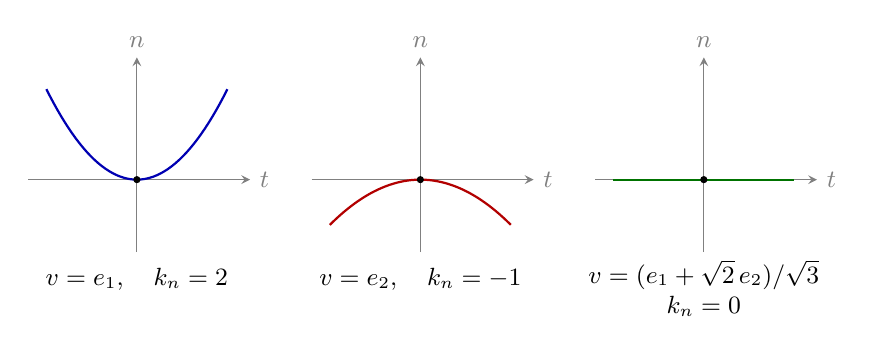
\begin{tikzpicture}[x=1.15cm,y=1.15cm,>=stealth,font=\small]
		\begin{scope}
			\draw[->,gray] (-1.2,0)--(1.25,0) node[right]{\(t\)};
			\draw[->,gray] (0,-0.8)--(0,1.35) node[above]{\(n\)};
			\draw[thick,blue!70!black,domain=-1:1,samples=50] plot(\x,{\x*\x});
			\fill (0,0) circle(1.3pt);
			\node at (0,-1.1){\(v=e_1,\quad k_n=2\)};
		\end{scope}
		\begin{scope}[xshift=3.6cm]
			\draw[->,gray] (-1.2,0)--(1.25,0) node[right]{\(t\)};
			\draw[->,gray] (0,-0.8)--(0,1.35) node[above]{\(n\)};
			\draw[thick,red!70!black,domain=-1:1,samples=50] plot(\x,{-0.5*\x*\x});
			\fill (0,0) circle(1.3pt);
			\node at (0,-1.1){\(v=e_2,\quad k_n=-1\)};
		\end{scope}
		\begin{scope}[xshift=7.2cm]
			\draw[->,gray] (-1.2,0)--(1.25,0) node[right]{\(t\)};
			\draw[->,gray] (0,-0.8)--(0,1.35) node[above]{\(n\)};
			\draw[thick,green!45!black] (-1,0)--(1,0);
			\fill (0,0) circle(1.3pt);
			\node[align=center] at (0,-1.2){\(v=(e_1+\sqrt2\,e_2)/\sqrt3\)\\\(k_n=0\)};
		\end{scope}
	\end{tikzpicture}
	\caption[鞍面在不同方向的法截线]{图像 \(z=x^2-\tfrac12y^2\) 在原点的三条法截线，各自画在由 \(v,n\) 张成的截平面内。三图的横坐标均沿单位切方向 \(v\)，纵坐标沿选定法向 \(n\)；相应截线为 \(z=t^2\)、\(z=-t^2/2\) 与 \(z=0\)。}
	\label{g1:fig:normal-sections}
\end{figure}


\subsection{平均曲率、Gauss 曲率及脐点}
\label{g1:subsec:0802:03}

两个主曲率交换编号时，和与积都不改变。把它们用于刻画曲面，可以避免不断选择和排列主方向。和反映两个正交方向的平均弯曲，积则区分同向弯曲、反向弯曲与二阶退化。

\begin{definition}[平均曲率、Gauss 曲率与脐点]\label{g1:def:surface-curvatures}
	在带选定单位法向的光滑浸入曲面上，定义\term[pingjunqulv]{平均曲率}[mean curvature]与\term[Gaussqulv]{Gauss 曲率}[Gaussian curvature]为
	\[
		H\coloneqq\tfrac12\operatorname{tr}S=\tfrac12(k_1+k_2),\qquad K\coloneqq\det S=k_1k_2.
	\]
	若某点 \(k_1=k_2\)，则称为\term[qidian]{脐点}[umbilic point]，等价地，该点 \(S=HI\)。若 \(S=0\)，称其为\term[pingdian]{平点}[planar point]；平点是两个主曲率都为零的脐点。
	\symidx{\(H\)：平均曲率}
	\symidx{\(K\)：曲面的 Gauss 曲率}
\end{definition}

这里的 \(1/2\) 属于平均曲率的约定，有些文献把主曲率之和直接叫作平均曲率。我们后续的公式均使用上面的平均值。Gauss 曲率目前是通过曲面在三维空间中的法向变化定义的；它是否也能仅由第一基本形式恢复，是下一节要证明的问题。

\begin{proposition}[曲率的计算与法向选择]\label{g1:prop:surface-curvature-formulas}
	设 \(X:U\to\mathbb R^3\) 是光滑浸入，选定单位法向，并使用第一、第二基本形式的系数 \(E,F,G,h_{ij}\)。则
	\begin{equation}\label{g1:eq:surface-HK-formulas}
		K=\frac{h_{11}h_{22}-h_{12}^2}{D},\qquad
		H=\frac{Gh_{11}-2Fh_{12}+Eh_{22}}{2D},\qquad D=EG-F^2.
	\end{equation}
	有 \(H^2-K\ge0\)，两个主曲率是 \(H\pm\sqrt{H^2-K}\)，脐点恰由 \(H^2=K\) 刻画。把法向改为 \(-n\) 时，\(S,\mathrm{II},H\) 同时变号，两个主曲率各自变号，\(K\) 与主方向不变。
\end{proposition}
\begin{proof}
	由\eqref{g1:eq:shape-matrix}，
	\[
		[S]=\frac1D
		\begin{pmatrix}
			Gh_{11}-Fh_{12}&Gh_{12}-Fh_{22}\\
			Eh_{12}-Fh_{11}&Eh_{22}-Fh_{12}
		\end{pmatrix}.
	\]
	取行列式和迹即得\eqref{g1:eq:surface-HK-formulas}。又
	\[
		H^2-K=\tfrac14(k_1-k_2)^2,\qquad
		\det(\lambda I-S)=\lambda^2-2H\lambda+K,
	\]
	所以平方根为实数，二次方程的根给出主曲率，等根恰为脐点。法向翻转后 \(S=-\mathrm dn\) 变号，其余各项由定义得到；若主曲率原先按大小排序，翻转后还须交换顺序。
\end{proof}

例如，外向法向的半径 \(R\) 球面处处有 \(H=-1/R\)、\(K=1/R^2\)，且每一点都是脐点。平面取任一固定单位法向则有 \(S=0\)。与此不同，图像 \(z=x^3-3xy^2\) 只在原点有二阶偏导全部为零，所以原点是平点；在其余位置，二阶偏导矩阵的行列式为 \(-36(x^2+y^2)\)，由图像公式及\eqref{g1:eq:surface-HK-formulas}知 \(K<0\)。因此“一点的第二基本形式为零”不意味着附近的曲面是一张平面。

\ProseParagraphBreak

平均曲率还真的是各方向法曲率的角平均。由 Euler 公式，
\[
	\frac1{2\pi}\int_0^{2\pi}k_n(\cos\theta\,e_1+\sin\theta\,e_2)\,\mathrm d\theta
	=\frac{k_1+k_2}2=H.
\]
平均值为零时，各方向的弯曲可能恰好抵消，不能据此断言每个方向都不弯曲。例如上一小节的鞍面若改为 \(z=x^2-y^2\)，则原点 \(H=0\) 而 \(K=-4\)。

\subsection{曲率线、渐近线及其退化}
\label{g1:subsec:0802:04}

一点上的方向能否沿曲面连成曲线，是另一个问题。先规定要沿哪些方向行走，再讨论方向能否光滑选取以及微分方程是否有解；这两步在脐点或曲率变号处都可能发生变化。

\begin{definition}[曲率线与渐近线]\label{g1:def:principal-asymptotic-curves}
	在带选定单位法向的光滑浸入曲面上，若一条光滑正则曲线的切向量处处为形算子的特征向量，称其为\term[qulvxian]{曲率线}[line of curvature]。若非零切向量 \(v\) 满足 \(\mathrm{II}(v,v)=0\)，称它张成的无向直线为\term[jianjinfangxiang]{渐近方向}[asymptotic direction]；切向量处处为渐近方向的光滑正则曲线称为\term[jianjinxian]{渐近线}[asymptotic curve]。
\end{definition}

法向翻转不改变特征方向，也不改变 \(\mathrm{II}(v,v)=0\) 的解，因此这两类曲线可以不依赖整体法向选择来讨论。曲率线要求法向变化 \(\mathrm dn(v)\) 与行进方向平行；渐近线要求曲线的法向加速度为零。两者是不同条件。

\begin{lemma}[局部积分曲线]\label{g1:lem:surface-field-integral-curve}
	设 \(V:U\to\mathbb R^2\) 是开集 \(U\subset\mathbb R^2\) 上的光滑向量场，\(u_0\in U\)。则在某个 \((-\varepsilon,\varepsilon)\) 上，初值问题
	\[
		\dot u(t)=V(u(t)),\qquad u(0)=u_0
	\]
	有唯一的局部光滑解。若 \(V(u_0)\ne0\)，缩小区间后该解正则。
\end{lemma}
\begin{proof}
	取闭球 \(\overline B(u_0,r)\subset U\)。由于 \(V\) 及其一阶导数在闭球上有界，存在常数 \(M,L\ge0\)，使 \(\lVert V\rVert\le M\) 且 \(\lVert V(x)-V(y)\rVert\le L\lVert x-y\rVert\)。选 \(a>0\) 足够小，使 \(aM<r\)、\(q=aL<1\)。在所有取值于此闭球的连续路径 \(u:[-a,a]\to\overline B(u_0,r)\) 上定义
	\[
		(\mathcal Tu)(t)=u_0+\int_0^t V(u(s))\,\mathrm ds.
	\]
	估计 \(aM<r\) 保证 \(\mathcal T\) 仍取值于闭球，而一致范数满足
	\[
		\lVert\mathcal Tu-\mathcal Tw\rVert_\infty\le q\lVert u-w\rVert_\infty.
	\]
	从常路径 \(u_0\) 迭代 \(u_{m+1}=\mathcal Tu_m\)，相邻两次的差至多按 \(q^m\) 衰减。几何级数收敛说明 \(u_m\) 一致收敛；连续路径的一致极限仍连续且取值于闭球。把极限送入积分，得到 \(u=\mathcal Tu\)，所以 \(u\) 为 \(C^1\) 且满足方程。若 \(u,w\) 都是这个积分方程的解，同一估计给出 \(\lVert u-w\rVert_\infty\le q\lVert u-w\rVert_\infty\)，因而两者相同。任意另一局部解在足够短的公共区间内也留在闭球中，这就给出局部唯一性。由 \(\dot u=V(u)\) 逐次求导，\(u\) 为光滑；最后用 \(V(u_0)\ne0\) 及连续性保证附近速度不消失。
\end{proof}

\begin{proposition}[主方向与渐近方向的局部曲线]\label{g1:prop:principal-asymptotic-lines}
	设 \(X:U\to\mathbb R^3\) 为光滑浸入。
	\begin{enumerate}
		\item 每个非脐点附近有两族局部曲率线；经过给定点、沿指定主方向的局部曲率线唯一到正则重参数化为止。
		\item 每个 \(K<0\) 的点附近有两族局部渐近线；经过给定点、沿指定渐近方向的局部渐近线唯一到正则重参数化为止。
		\item 在一点，若 \(K>0\)，没有渐近方向；若 \(K<0\)，有两条不同的渐近方向；若 \(K=0\) 且 \(S\ne0\)，恰有一条渐近方向，为 \(\ker S\)；若 \(S=0\)，所有方向都是渐近方向。
	\end{enumerate}
\end{proposition}
\begin{proof}
	在非脐点附近，\(H^2-K>0\)。所以
	\[
		k_+=H+\sqrt{H^2-K},\qquad k_-=H-\sqrt{H^2-K}
	\]
	是光滑的不同特征值。相应的线性算子
	\[
		P_+=\frac{S-k_-I}{k_+-k_-},\qquad P_-=\frac{S-k_+I}{k_--k_+}
	\]
	分别投影到两条特征直线上。先取一个光滑切向量场 \(W\)，使 \(P_+W\) 在指定点不为零；例如把该点的一个特征向量按坐标基用常系数延伸。缩小邻域后 \(P_+W\) 始终不为零，归一化得到光滑单位特征向量场 \(e_+\)。同理得到 \(e_-\)，并可按需要调整其符号。把 \(e_+\) 在 \(X_1,X_2\) 下的系数看作 \(U\) 上的非零光滑向量场，应用\cref{g1:lem:surface-field-integral-curve}并复合 \(X\)，即得所需曲率线。另一主方向同样处理。任意沿同一方向的正则曲线，缩短后可调整方向并改用弧长，使其导数等于所选单位场；初值唯一性就给出无参数轨迹的唯一性。

	当 \(K<0\) 时，\(k_+>0>k_-\)。在上面选出的光滑正交单位场中，二次型的零方向由
	\[
		k_+a^2+k_-b^2=0
	\]
	确定，分别由两个光滑非零场
	\[
		\sqrt{-k_-}\,e_++\sqrt{k_+}\,e_-,
		\qquad
		\sqrt{-k_-}\,e_+-\sqrt{k_+}\,e_-
	\]
	张成。归一化后再次应用局部积分曲线引理，得到存在与唯一性。

	最后，在任一点用主方向正交基把 \(\mathrm{II}\) 写成 \(k_1a^2+k_2b^2\)。若两系数同号，此式对非零向量不为零；若异号，得到上面的两条直线；若恰有一个系数为零，解是一条坐标轴；若两者都为零，每个向量都是解。这证明了第三项。
\end{proof}

这份分类只需解一个二元二次方程，可整理为\cref{g1:tab:asymptotic-directions}。其中 \(K=0\) 的两行必须分开：仅凭 \(K\) 的值，无法判断零方向是一条还是所有方向。

\begin{table}[htbp]
	\centering
	\caption{第二基本形式与渐近方向}
	\label{g1:tab:asymptotic-directions}
	\begin{tabular}{lll}
		\toprule
		条件 & 主方向基下的二次型 & 渐近方向 \\
		\midrule
		\(K>0\) & 两个非零系数同号 & 无 \\
		\(K<0\) & 两个系数异号 & 两条不同直线 \\
		\(K=0,\ S\ne0\) & 恰有一个系数为零 & 一条直线 \\
		\(S=0\) & 零二次型 & 所有方向 \\
		\bottomrule
	\end{tabular}
\end{table}

在一整片 \(K=0,\ S\ne0\) 的区域上，零特征值与另一个特征值仍然分离，上面的投影构造同样给出一条光滑方向场及其积分曲线。但若只知道某一点 \(K=0\)，不能据此断言有渐近线穿过它。例如 \(z=x^2+y^4\) 在原点的形算子为 \(\operatorname{diag}(2,0)\)，只有 \(y\) 轴方向渐近；在 \(y\ne0\) 处却有 \(K>0\)，不存在渐近方向。若有正则渐近线通过原点，其速度必须沿 \(y\) 轴且不为零，于是附近离开原点后 \(y\ne0\)，矛盾。因此原点的渐近方向不能延续成穿过该点的渐近线。

\ProseParagraphBreak

脐点处的困难则是主方向不再分离。球面的每条正则曲线都是曲率线，经过一点和一条切向的曲线远不唯一。即使避开脐点，在一张较大的曲面上也不能从局部单位特征向量的选择自动得到全局连续选择：沿闭路延伸后，向量可能反向，而它张成的直线仍相同。曲率线和渐近线的定义使用无向直线，正是为了把这种方向选择与曲线本身区别开。

% !TeX root = ../../Book1.tex
% 纲要标题：### 8.3 结构方程与内在曲率
% 纲要位置：几何学计划纲要.md，第 416 行。
% 正文状态：初稿；尚未正式审核。

% 纲要内容开始
% 
% * Gauss–Weingarten 方程
% * 协变导数与 Christoffel 系数
% * Gauss 方程与绝妙定理
% * Codazzi 方程及混合偏导相容性
% 
% 纲要内容结束

\section{结构方程与内在曲率}
\label{g1:sec:0803}

第一基本形式记录切平面中的长度，第二基本形式记录曲面向法向弯曲的程度。它们看起来各管一件事，但不能任意指定：如果它们来自同一个位置函数 \(X(u,v)\)，先对 \(u\) 求导再对 \(v\) 求导，必须与相反的顺序得到相同结果。这一简单要求将同时给出 Gauss 方程和 Codazzi 方程。Gauss 方程还将把主曲率的乘积写成第一基本形式及其导数的表达式，将法向弯曲与内在度量联系起来。

\ProseParagraphBreak

本节取光滑浸入 \(X\colon U\rightarrow\mathbb R^3\)，其中 \(U\subseteq\mathbb R^2\) 开，记 \(u^1=u\)、\(u^2=v\)、\(X_i=\partial_iX\)。沿用 \(g_{ij}=\langle X_i,X_j\rangle\)、\(D=\det(g_{ij})>0\) 与选定的单位法向 \(n\)，并记 \(h_{ij}=\langle X_{ij},n\rangle\)。向量场及其导数都按参数点定义；若像有自交，不把不同参数点上的切向量混为一谈。指标 \(i,j,k,\ell,m\) 均取 \(1,2\)；在同一项中重复出现的一上一下指标表示对这两个值求和。这个简写只省去求和号，不改变矩阵的乘法顺序。

\subsection{Gauss–Weingarten 方程}
\label{g1:subsec:0803:01}

前一节已经把 \(X_{ij}\) 的法向分量写成 \(h_{ij}n\)。剩下的切向分量也需要记录，因为坐标向量 \(X_1,X_2\) 一般随位置改变，既不保持长度，也不保持夹角。令 \((g^{ij})\) 为 \((g_{ij})\) 的逆矩阵，并写 \(h_i{}^k=g^{k\ell}h_{i\ell}\)。

\begin{proposition}[Gauss–Weingarten 方程]
	\label{g1:prop:gauss-weingarten}
	设 \(U\subseteq\mathbb R^2\) 开，\(X:U\rightarrow\mathbb R^3\) 是光滑浸入，\(n\) 为光滑单位法向。记 \(X_i=\partial_iX\)、\(g_{ij}=\langle X_i,X_j\rangle\)、\(h_{ij}=\langle\partial_i\partial_jX,n\rangle\)、\((g^{ij})=(g_{ij})^{-1}\)，并令 \(h_i{}^k=\sum_\ell g^{k\ell}h_{i\ell}\)。重复指标取 \(1,2\) 并求和。存在唯一的光滑函数 \(\Gamma^k_{ij}\)，使
	\begin{equation}
		\label{g1:eq:gauss-weingarten}
		\partial_iX_j=\Gamma^k_{ij}X_k+h_{ij}n,\qquad
		\partial_i n=-h_i{}^kX_k.
	\end{equation}
	其中 \(\Gamma^k_{ij}=\Gamma^k_{ji}\)，并且
	\begin{equation}
		\label{g1:eq:christoffel-metric}
		\Gamma^k_{ij}
		=\frac12g^{k\ell}\bigl(\partial_i g_{j\ell}+\partial_j g_{i\ell}-\partial_\ell g_{ij}\bigr).
	\end{equation}
	因此 \(X_{ij}\) 的切向分解系数完全由第一基本形式决定。
\end{proposition}

\begin{proof}
	浸入条件保证 \(X_1,X_2,n\) 线性无关，所以向量 \(X_{ij}\) 有唯一的上述分解。混合偏导相等给出 \(\Gamma^k_{ij}=\Gamma^k_{ji}\)。对 \(g_{j\ell}=\langle X_j,X_\ell\rangle\) 求导，得到
	\[
		\partial_i g_{j\ell}=\langle X_{ij},X_\ell\rangle+\langle X_j,X_{i\ell}\rangle.
	\]
	把交换 \(i,j,\ell\) 所得的三个式子按前两个相加、第三个相减，交叉项抵消，故
	\[
		2\langle X_{ij},X_\ell\rangle
		=\partial_i g_{j\ell}+\partial_j g_{i\ell}-\partial_\ell g_{ij}
		=2\Gamma^k_{ij}g_{k\ell}.
	\]
	乘逆矩阵便得\eqref{g1:eq:christoffel-metric}。

	由 \(\langle n,n\rangle=1\) 可知 \(\partial_i n\) 是切向量；对 \(\langle n,X_j\rangle=0\) 求导，又有
	\[
		\langle\partial_i n,X_j\rangle=-\langle n,X_{ij}\rangle=-h_{ij}.
	\]
	若 \(\partial_i n=a^kX_k\)，则 \(a^kg_{kj}=-h_{ij}\)，即 \(a^k=-g^{k\ell}h_{i\ell}\)。
\end{proof}

\eqref{g1:eq:gauss-weingarten}中的第一式称为 Gauss 公式，第二式称为 Weingarten 公式；两式合称\term[gaussweingartenfangcheng]{Gauss–Weingarten 方程}[Gauss--Weingarten equations]。第二式正是形算子 \(S=-\mathrm{d}n\) 的坐标表达；负号与\cref{g1:def:shape-operator}的约定一致。\footnote{Weingarten，Julius Weingarten（1836--1910），德国数学家，研究曲面等距变形与曲率线。}

\ProseParagraphBreak

这里的标架 \((X_1,X_2,n)\) 通常不是正交单位标架。因此 \(\Gamma^k_{ij}\) 无须像\eqref{g1:eq:frenet-matrix}中的系数矩阵那样斜对称。其作用是补偿坐标基自身的变化；这个变化有些来自曲面的弯曲，有些仅来自选了弯曲的坐标线。

\subsection{协变导数与 Christoffel 系数}
\label{g1:subsec:0803:02}

设 \(V=V^iX_i\) 是沿曲面的光滑切向量场。把它当作取值于 \(\mathbb R^3\) 的函数求导，\(\partial_iV\) 未必仍在切平面内。例如球面上的切向量沿曲线变化时，普通导数可能含有径向分量。如果我们只记录曲面自身的切向变化，就应把普通导数投影回当前切平面。

\begin{definition}
	\label{g1:def:surface-covariant-derivative}
	设 \(U\subseteq\mathbb R^2\) 开，\(X:U\rightarrow\mathbb R^3\) 为光滑浸入，\(X_i=\partial_iX\)，\(V=V^iX_i\)、\(W=W^iX_i\) 为沿 \(X\) 的光滑切向量场，\(f\in C^\infty(U)\)，\(\Gamma^k_{ij}\) 为诱导度量的 Christoffel 系数。定义它沿坐标方向的\term[xiebiandaoshu]{协变导数}[covariant derivative]为
	\[
		\nabla_iV\coloneqq(\partial_iV)^\top
		=\bigl(\partial_iV^k+\Gamma^k_{ij}V^j\bigr)X_k,
	\]
	其中 \({}^\top\) 表示向切平面的正交投影。若 \(W=W^iX_i\)，则定义 \(\nabla_WV=W^i\nabla_iV\)。函数的方向导数记为 \(W(f)=W^i\partial_i f\)。\symidx{\(\nabla_WV\)：切向量场的协变导数}
\end{definition}

上式中的 \(\Gamma^k_{ij}\) 称为\term[christoffelxishu]{Christoffel 系数}[Christoffel symbols]，也称 Christoffel 符号。\footnote{Christoffel，Elwin Bruno Christoffel（1829--1900），德国数学家，研究二次微分形式、张量演算与共形映射。}在这里“协变”所强调的是：重参数化后，计算仍给出同一个切向量，而非要求各个数 \(\Gamma^k_{ij}\) 保持不变。定义中的正交投影及方向导数都是几何操作，已经说明其不依赖坐标；公式中新增的 \(\Gamma^k_{ij}V^j\) 恰好补上了基向量求导的部分。\symidx{\(\Gamma^k_{ij}\)：Christoffel 系数}

\begin{example}[平面也可以有非零的 Christoffel 系数]
	\label{g1:exm:polar-christoffel}
	在平面的极坐标参数 \(X(r,\theta)=(r\cos\theta,r\sin\theta,0)\) 中，取 \(r>0\) 及一个适当的角度区间，有 \(g_{rr}=1\)、\(g_{r\theta}=0\)、\(g_{\theta\theta}=r^2\)。代入\eqref{g1:eq:christoffel-metric}得到仅有的非零系数
	\[
		\Gamma^r_{\theta\theta}=-r,\qquad
		\Gamma^\theta_{r\theta}=\Gamma^\theta_{\theta r}=\frac1r.
	\]
	例如 \(\partial_\theta X_\theta=-rX_r\) 只是平面内的径向加速度，并不意味着平面发生了法向弯曲。在直角坐标下，同一平面的全部 Christoffel 系数都为零。
\end{example}

这种现象说明 \(\Gamma^k_{ij}\) 不是一个张量的分量：如果张量在某组基下全部分量为零，换基后仍应全部为零。更直接地，设新坐标为 \(y^a\)，旧坐标为 \(u^i=u^i(y)\)，对 \(\widetilde X(y)=X(u(y))\) 求两次导数，并比较切向分量，得到
\[
	\widetilde\Gamma^c_{ab}
	=\frac{\partial y^c}{\partial u^k}
	\left(
		\Gamma^k_{ij}\frac{\partial u^i}{\partial y^a}\frac{\partial u^j}{\partial y^b}
		+\frac{\partial^2u^k}{\partial y^a\partial y^b}
	\right).
\]
最后的二阶导数项不是逐点线性换基产生的项。协变导数整体仍然与坐标无关，因为向量分量 \(V^i\) 的导数也发生变化，恰好抵消这项。

\ProseParagraphBreak

为了比较先沿两个方向求导的结果，需要注意：任意两个向量场的方向导数未必可交换。定义它们的\term[xiangliangchangkuohao]{向量场括号}[Lie bracket]为
\[
	[W,V]=\bigl(W^i\partial_iV^k-V^i\partial_iW^k\bigr)X_k.
\]
对每个光滑函数 \(f\)，直接展开可得 \([W,V](f)=W(V(f))-V(W(f))\)，其中二阶偏导项成对抵消。这也给出了括号与坐标无关的含义。这一运算也称为 Lie 括号。\footnote{Lie，Marius Sophus Lie（1842--1899），挪威数学家，创立连续变换群理论，并研究其与微分方程的联系。}特别地，坐标向量场满足 \([X_1,X_2]=0\)；这并不是说作为 \(\mathbb R^3\) 值函数的 \(X_1,X_2\) 是常向量。

\begin{proposition}[切向求导的基本性质]
	\label{g1:prop:surface-connection-properties}
	设 \(U\subseteq\mathbb R^2\) 开，\(X:U\to\mathbb R^3\) 为光滑浸入，\(\nabla_WV\) 由普通方向导数沿 \(W\) 求导后向切平面正交投影得到。此协变导数对向量场可加，且对任意光滑函数 \(f\) 及切向量场 \(V,W,Z\)，有
	\begin{align*}
		\nabla_{fW}V&=f\nabla_WV,&
		\nabla_W(fV)&=W(f)V+f\nabla_WV,\\
		W\langle V,Z\rangle&=\langle\nabla_WV,Z\rangle+\langle V,\nabla_WZ\rangle,&
		\nabla_WV-\nabla_VW&=[W,V].
	\end{align*}
	后两条分别称为\term[duliangxiangrong]{度量相容}[metric compatibility]和\term[wunao]{无挠性}[torsion-freeness]。更一般地，在开集 \(U\subseteq\mathbb R^2\) 上给定任意光滑正定矩阵场 \(g=(g_{ij})\)，令 \((g^{ij})=(g_{ij})^{-1}\)，按 Christoffel 公式\eqref{g1:eq:christoffel-metric}，即 \(\Gamma^k_{ij}=\tfrac12g^{k\ell}(\partial_i g_{j\ell}+\partial_j g_{i\ell}-\partial_\ell g_{ij})\)，及 \(\nabla_WV=W^i(\partial_iV^k+\Gamma^k_{ij}V^j)\partial_k\) 定义的运算也满足这两条性质，而且它是满足这些性质与前两条求导规则的唯一运算。
\end{proposition}

\begin{proof}
	前两条由普通求导的线性及乘法法则得到。对于诱导度量，普通内积求导后出现的法向分量与 \(V,Z\) 垂直，所以投影不改变结果，得到度量相容。再展开 \(\nabla_WV-\nabla_VW\)，由于 \(\Gamma^k_{ij}=\Gamma^k_{ji}\)，所有含 \(\Gamma\) 的项相消，余项就是括号。

	对于任意给定的正定 \(g\)，公式\eqref{g1:eq:christoffel-metric}仍给出 \(\Gamma^k_{ij}=\Gamma^k_{ji}\)，所以无挠性的证明不变。另有
	\[
		\Gamma^k_{ij}g_{k\ell}+\Gamma^k_{i\ell}g_{jk}
		=\partial_i g_{j\ell},
	\]
	因为将右式中的两个 \(\Gamma\) 换成定义后，其余偏导项互相抵消。这正是对坐标向量场的度量相容，乘以向量场分量并用乘法法则即得一般情形。

	最后，设另一运算满足相同规则，写其坐标系数为 \(C^k_{ij}\)。无挠性给出 \(C^k_{ij}=C^k_{ji}\)，度量相容给出 \(\partial_i g_{j\ell}=C^k_{ij}g_{k\ell}+C^k_{i\ell}g_{jk}\)。如\cref{g1:prop:gauss-weingarten}的证明那样将三个式子相加减，就强制得到 \(C^k_{ij}=\Gamma^k_{ij}\)。
\end{proof}

这一运算也称为度量的\term[lianluo]{联络}[connection]。在只给定 \(g\) 而尚未构造曲面时，我们把坐标基写作 \(\partial_1,\partial_2\)，完全可以照同一公式求导。重参数化后，度量相容、无挠性和两条求导规则都保持；上面的唯一性说明，各套坐标得到的是同一个运算。因此，“把普通导数投影回去”是诱导度量的直观构造，“由 \(g\) 的系数求出 \(\Gamma\)”则使这个构造不再依赖于周围的三维空间。

\subsection{Gauss 方程与绝妙定理}
\label{g1:subsec:0803:03}

普通二阶偏导可交换，协变二阶导数却是在每次求导后都投影一次，两次中间使用的切平面不同，结果可能不同。若方向本身也是变化的向量场，还必须扣除它们的括号造成的差别。扣除这一差别后，结果才能只依赖给定点上的方向。

\begin{definition}
	\label{g1:def:surface-curvature-tensor}
	设 \((M,g)\) 为光滑度量曲面，\(\nabla\) 为 \(g\) 的无挠相容协变导数。对任意光滑切向量场 \(V,W,Z\)，定义
	\[
		R(V,W)Z\coloneqq\nabla_V\nabla_WZ-\nabla_W\nabla_VZ-\nabla_{[V,W]}Z.
	\]
	这个运算称为\term[qulvzhangliang]{曲率张量}[curvature tensor]。本书固定上述符号顺序。\symidx{\(R(V,W)Z\)：曲率张量}
\end{definition}

\begin{proposition}
	\label{g1:prop:curvature-tensorial}
	设 \(M\) 为光滑曲面，\(\nabla\) 为其切丛上的光滑联络，\(V,W,Z\) 为光滑切向量场。令 \(R(V,W)Z=\nabla_V\nabla_WZ-\nabla_W\nabla_VZ-\nabla_{[V,W]}Z\)，此处不要求联络无挠或与度量相容。则 \(R(V,W)Z\) 对三个向量场均为逐点线性：任意光滑函数 \(f\) 均满足
	\begin{align*}
		R(fV,W)Z&=fR(V,W)Z,\\
		R(V,fW)Z&=fR(V,W)Z,\\
		R(V,W)(fZ)&=fR(V,W)Z.
	\end{align*}
	因此在点 \(p\) 的值只依赖 \(V(p),W(p),Z(p)\)，不依赖这些向量在邻域中的延拓。
\end{proposition}

\begin{proof}
	先由括号的坐标式得到 \([fV,W]=f[V,W]-W(f)V\)。代入定义，第二项求导产生的 \(-W(f)\nabla_VZ\) 正好与括号项中的 \(W(f)\nabla_VZ\) 抵消，证明第一式。由 \(R(W,V)=-R(V,W)\) 得第二式。

	对第三式，把两次乘法法则代入定义。含 \(\nabla_VZ,\nabla_WZ\) 的一阶导数项成对抵消，剩余的额外项只有
	\[
		\bigl(V(W(f))-W(V(f))-[V,W](f)\bigr)Z=0.
	\]
	故第三式成立。将三个向量场各自在坐标基中展开，所得值是各自分量在 \(p\) 的乘积乘以 \(R(X_i,X_j)X_k\) 在 \(p\) 的值，所以确实只需要三个输入向量的点值。
\end{proof}

这里“张量”的具体含义是：在每一点，这个多线性映射都把三个切向量映为一个切向量。

\ProseParagraphBreak

由于 \([X_1,X_2]=0\)，计算坐标分量只须展开两次求导：
\begin{equation}
	\label{g1:eq:surface-curvature-components}
	\begin{aligned}
		R(X_1,X_2)X_j&=R^k{}_{j12}X_k,\\
		R^k{}_{j12}
		&=\partial_1\Gamma^k_{2j}-\partial_2\Gamma^k_{1j}
		+\Gamma^k_{1m}\Gamma^m_{2j}-\Gamma^k_{2m}\Gamma^m_{1j}.
	\end{aligned}
\end{equation}
例如 \(\nabla_1(\Gamma^m_{2j}X_m)\) 同时对系数及基向量求导，才得到偏导项和两个系数的乘积。遗漏后一部分，就会把坐标基变化误当作曲率。

\begin{theorem}[Gauss 方程]
	\label{g1:thm:gauss-equation}
	设 \(U\subseteq\mathbb R^2\) 开，\(X:U\rightarrow\mathbb R^3\) 是光滑浸入，取光滑单位法向 \(n\)，形算子为 \(S=-\mathrm{d}n\)，第二基本形式为 \(h(V,W)=\langle SV,W\rangle\)。以 \(\nabla\) 记诱导度量的无挠相容协变导数，定义 \(R(V,W)Z=\nabla_V\nabla_WZ-\nabla_W\nabla_VZ-\nabla_{[V,W]}Z\)，其中 \(V,W,Z\) 为光滑切向量场。令 \(X_i=\partial_iX\)、\(g_{ij}=\langle X_i,X_j\rangle\)、\((g^{ij})=(g_{ij})^{-1}\)、\(h_{ij}=h(X_i,X_j)\)、\(h_i{}^k=g^{k\ell}h_{i\ell}\)，并以 \(R(X_1,X_2)X_j=R^k{}_{j12}X_k\) 定义曲率分量。则曲率满足
	\begin{equation}
		\label{g1:eq:gauss-equation}
		R(V,W)Z=h(W,Z)SV-h(V,Z)SW.
	\end{equation}
	特别地，
	\[
		R^k{}_{j12}=h_{2j}h_1{}^k-h_{1j}h_2{}^k,\qquad
		\langle R(X_1,X_2)X_2,X_1\rangle=h_{11}h_{22}-h_{12}^2.
	\]
\end{theorem}

\begin{proof}
	记 \(\mathrm{D}_V\) 为对 \(\mathbb R^3\) 值函数逐分量作方向导数。由定义及\cref{g1:prop:gauss-weingarten}，任意切向量场满足
	\[
		\mathrm{D}_VZ=\nabla_VZ+h(V,Z)n,\qquad \mathrm{D}_Vn=-SV.
	\]
	Euclid 空间中的逐分量求导满足
	\[
		\mathrm{D}_V\mathrm{D}_WZ-\mathrm{D}_W\mathrm{D}_VZ-\mathrm{D}_{[V,W]}Z=0,
	\]
	因为对每个分量这正是括号的定义。将前两个分解式代入，并只取切向分量：
	\[
		0=\nabla_V\nabla_WZ-h(W,Z)SV
		-\nabla_W\nabla_VZ+h(V,Z)SW-\nabla_{[V,W]}Z.
	\]
	移项便得 Gauss 方程。最后取 \(V=X_1,W=Z=X_2\)，再与 \(X_1\) 作内积，使用 \(h(X_i,X_j)=h_{ij}\)，即可得到坐标结论。
\end{proof}

上面的等式称为\term[gaussfangcheng]{Gauss 方程}[Gauss equation]。左边只由度量求导得到，右边却是法向弯曲的数据。由\cref{g1:prop:surface-curvature-formulas}，\(K=\det(h_{ij})/\det(g_{ij})\)，因此立即得到
\begin{equation}
	\label{g1:eq:intrinsic-gauss-curvature}
	K=\frac{\langle R(X_1,X_2)X_2,X_1\rangle}{D}
	=\frac{g_{1k}R^k{}_{212}}{D}.
\end{equation}
其右端只使用 \(g_{ij}\)、它们的逆矩阵和一二阶偏导数。

\begin{theorem}[Gauss 绝妙定理]
	\label{g1:thm:theorema-egregium}
	光滑曲面的 Gauss 曲率由第一基本形式决定。若两个光滑正则曲面片局部等距，则对应点的 Gauss 曲率相等；此结论不要求局部等距来自三维 Euclid 空间的刚性变换，也不要求保持所选法向。
\end{theorem}

\begin{proof}
	设局部等距在参数域中由微分同胚 \(\phi\) 表示。用 \(\phi\) 重参数化第二个曲面片后，它与第一个曲面片的 \(g_{ij}\) 完全相同，因而\eqref{g1:eq:christoffel-metric}给出相同的 \(\Gamma^k_{ij}\)，\eqref{g1:eq:surface-curvature-components}给出相同的 \(R^k{}_{j12}\)。再由\eqref{g1:eq:intrinsic-gauss-curvature}，两者的 \(K\) 相同。反转法向虽使 \(h,S\) 变号，却不改变 \(\det S\)，所以结论也不依赖该选择。
\end{proof}

这一定理称为\term[juemiaodingli]{绝妙定理}[theorema egregium]。内在度量确定两主曲率的乘积；平面与圆柱可以局部等距而主曲率不同，说明单个主曲率还记录着外在弯曲。另一方面，标准球面有 \(K=1/R^2\)，平面有 \(K=0\)，所以球面上任何开片都不能通过保持长度的局部等距完全铺到平面上。

\ProseParagraphBreak

下一节将从给定的度量与对称形式出发，尚无曲面可供求导。为此要明确：二维度量的曲率也只有一个独立的数，因而一个标量 Gauss 方程足以表达全部曲率条件。

\begin{proposition}[二维曲率只有一个独立分量]
	\label{g1:prop:surface-curvature-two-dim}
	设 \(g\) 是开集 \(U\subseteq\mathbb R^2\) 上的光滑正定度量，令 \((g^{ij})=(g_{ij})^{-1}\)，按\eqref{g1:eq:christoffel-metric}，即 \(\Gamma^k_{ij}=\tfrac12g^{k\ell}(\partial_i g_{j\ell}+\partial_jg_{i\ell}-\partial_\ell g_{ij})\)，定义 \(\nabla_i\partial_j=\Gamma^k_{ij}\partial_k\)，并令 \(R(V,W)Z=\nabla_V\nabla_WZ-\nabla_W\nabla_VZ-\nabla_{[V,W]}Z\)。令
	\[
		K_g\coloneqq\frac{g(R(\partial_1,\partial_2)\partial_2,\partial_1)}
		{\det(g_{ij})}.
	\]
	则 \(K_g\) 不依赖坐标，且任意切向量 \(V,W,Z\) 都满足
	\begin{equation}
		\label{g1:eq:two-dimensional-curvature}
		R(V,W)Z=K_g\bigl(g(W,Z)V-g(V,Z)W\bigr).
	\end{equation}
	若另给 \(U\) 上的一个光滑对称双线性形式 \(h\)，令 \(S=g^{-1}h\)，则标量等式 \(K_g=\det S\) 等价于完整的 Gauss 方程\eqref{g1:eq:gauss-equation}。
\end{proposition}

\begin{proof}
	固定一点，令 \(C(V,W,Z,T)=g(R(V,W)Z,T)\)。定义给出 \(C\) 在前两个变量中反对称。度量相容又给出
	\[
		g(R(V,W)Z,T)+g(Z,R(V,W)T)=0.
	\]
	要验证这式，只须对 \(g(Z,T)\) 应用恒等式 \(VW-WV-[V,W]=0\)，每次用度量相容展开；含一次协变导数的交叉内积抵消，剩余的正是这两项。因此 \(C\) 在最后两个变量中也反对称。

	取该点的任意正交单位基 \(e_1,e_2\)。二维空间的交替双线性形式只有一个独立分量：若 \(V=ae_1+be_2\)、\(W=ce_1+de_2\)，则前两个位置按双线性与反对称性展开后只剩系数 \(ad-bc\)。对最后两个位置作同样展开，整个 \(C\) 就由
	\[
		k=C(e_1,e_2,e_2,e_1)
	\]
	决定。具体地，
	\[
		C(V,W,Z,T)=k\bigl(g(W,Z)g(V,T)-g(V,Z)g(W,T)\bigr).
	\]
	取 \(V=\partial_1,W=Z=\partial_2,T=\partial_1\)，括号内是 \(g_{11}g_{22}-g_{12}^2\)，故 \(k=K_g\)，同时得到\eqref{g1:eq:two-dimensional-curvature}。右式也表明，在任意另一组基上用同一比值求出的仍是 \(k\)，所以与坐标无关。

	最后，\(S=g^{-1}h\) 关于 \(g\) 自伴。在一点选取它的正交单位特征基，设特征值为 \(a,b\)。此时直接在基向量上计算可得
	\[
		h(W,Z)SV-h(V,Z)SW
		=ab\bigl(g(W,Z)V-g(V,Z)W\bigr).
	\]
	两边对 \(V,W,Z\) 多线性，因此对任意向量成立。又 \(ab=\det S\)，与已证公式比较便得到等价性。
\end{proof}

这里的 \(K_g\) 可以在尚未证明度量能够浸入 \(\mathbb R^3\) 时定义。若确有这样的浸入，Gauss 方程才把它与外在定义的 \(K=\det S\) 认作同一个函数。这一区别会在给定数据的实现问题中起作用。

\begin{example}[共形坐标中的内在曲率]
	\label{g1:exm:conformal-curvature}
	设在参数域上给定度量
	\[
		g=e^{2\phi(u,v)}(\mathrm du^2+\mathrm dv^2),
	\]
	其中 \(\phi\) 光滑。两坐标方向垂直，且长度按同一倍数缩放。由\eqref{g1:eq:christoffel-metric}，
	\[
		\begin{array}{lll}
			\Gamma^1_{11}=\phi_u,&\Gamma^1_{12}=\Gamma^1_{21}=\phi_v,&\Gamma^1_{22}=-\phi_u,\\
			\Gamma^2_{11}=-\phi_v,&\Gamma^2_{12}=\Gamma^2_{21}=\phi_u,&\Gamma^2_{22}=\phi_v.
		\end{array}
	\]
	计算 \(R^1{}_{212}\) 时，两个乘积和恰好抵消：
	\[
		R^1{}_{212}
		=-\phi_{uu}-\phi_{vv}
		+\bigl(-\phi_u^2+\phi_v^2\bigr)
		-\bigl(\phi_v^2-\phi_u^2\bigr)
		=-\phi_{uu}-\phi_{vv}.
	\]
	由于 \(g_{12}=0\)、\(g_{11}=e^{2\phi}\)、\(D=e^{4\phi}\)，得到
	\begin{equation}
		\label{g1:eq:conformal-gauss-curvature}
		K_g=-e^{-2\phi}(\phi_{uu}+\phi_{vv}).
	\end{equation}
	例如 \(\phi=\log2-\log(1+u^2+v^2)\) 时，\(\phi_{uu}+\phi_{vv}=-4/(1+u^2+v^2)^2\)，故 \(K_g=1\)。求出这个数不需要先构造法向或主曲率。
\end{example}

\subsection{Codazzi 方程及混合偏导相容性}
\label{g1:subsec:0803:04}

Gauss 方程比较的是二阶求导的切向部分。法向部分也必须相等，而其中包含的是 \(h_{ij}\) 的一阶变化。直接比较 \(\partial_1h_{2j}\) 与 \(\partial_2h_{1j}\) 还不够，因为 \(h\) 的两个输入基向量也随位置改变，需要把这两种变化扣除。

\begin{definition}
	\label{g1:def:covariant-h-derivative}
	设 \((M,g)\) 为光滑度量曲面，\(\nabla\) 为其无挠相容协变导数，\(h\) 为 \(M\) 上的光滑对称双线性形式。对光滑切向量场 \(V,W,Z\)，定义
	\[
		(\nabla_Vh)(W,Z)
		\coloneqq V\bigl(h(W,Z)\bigr)-h(\nabla_VW,Z)-h(W,\nabla_VZ).
	\]
	在局部坐标中，令 \(h_{jk}=h(\partial_j,\partial_k)\)、\(\nabla_i\partial_j=\Gamma^m_{ij}\partial_m\)，其坐标分量记为
	\[
		\nabla_i h_{jk}\coloneqq\partial_i h_{jk}
		-\Gamma^m_{ij}h_{mk}-\Gamma^m_{ik}h_{jm}.
	\]
\end{definition}

这个定义中的两个减项分别对应 \(h\) 的两个输入。利用协变导数的乘法法则可以检查：将 \(W\) 或 \(Z\) 换成 \(fW\) 或 \(fZ\)，求导产生的 \(V(f)\) 项被相应减项抵消；对 \(V\) 则直接逐点线性。因此 \(\nabla h\) 的值同样不依赖输入向量场的延拓。

\begin{theorem}[Codazzi 方程]
	\label{g1:thm:codazzi-equation}
	设 \(U\subseteq\mathbb R^2\) 开，\(X:U\rightarrow\mathbb R^3\) 是光滑浸入，\(n\) 为光滑单位法向，\(h\) 为相应第二基本形式，\(S=-\mathrm{d}n\) 为形算子，\(\nabla\) 为诱导度量的无挠相容协变导数，则
	\[
		(\nabla_Vh)(W,Z)=(\nabla_Wh)(V,Z)
	\]
	对任意光滑切向量场 \(V,W,Z\) 成立。在局部坐标中，令 \(h_{ij}=h(\partial_i,\partial_j)\)、\(\nabla_i\partial_j=\Gamma^m_{ij}\partial_m\)，坐标表达为两个方程
	\begin{equation}
		\label{g1:eq:codazzi-components}
		\nabla_1h_{2j}-\nabla_2h_{1j}
		=\partial_1h_{2j}-\partial_2h_{1j}
		+\Gamma^m_{2j}h_{1m}-\Gamma^m_{1j}h_{2m}=0,
		\qquad j=1,2.
	\end{equation}
	若定义 \((\nabla_VS)W=\nabla_V(SW)-S(\nabla_VW)\)，则同一条件也可写成 \((\nabla_VS)W=(\nabla_WS)V\)。
\end{theorem}

\begin{proof}
	对 Gauss–Weingarten 方程求一次偏导。由于 \(\partial_i n\) 与 \(n\) 垂直，
	\[
		\langle\partial_1\partial_2X_j,n\rangle
		=\Gamma^m_{2j}h_{1m}+\partial_1h_{2j},\qquad
		\langle\partial_2\partial_1X_j,n\rangle
		=\Gamma^m_{1j}h_{2m}+\partial_2h_{1j}.
	\]
	混合偏导相等立即给出\eqref{g1:eq:codazzi-components}。它与协变导数的表达相同，是因为展开 \(\nabla_1h_{2j}-\nabla_2h_{1j}\) 后，项 \(-\Gamma^m_{12}h_{mj}\) 与 \(+\Gamma^m_{21}h_{mj}\) 相消。其余恰为上式。前面已经证明 \(\nabla h\) 对三个输入逐点线性，所以在坐标基上验证便给出一般向量场的结论。

	最后，度量相容以及 \(h(W,Z)=g(SW,Z)\) 给出
	\[
		(\nabla_Vh)(W,Z)
		=g\bigl(\nabla_V(SW)-S(\nabla_VW),Z\bigr).
	\]
	因度量非退化，对所有 \(Z\) 的内积相等当且仅当对应向量相等，这就得到形算子形式。
\end{proof}

这些关系称为\term[codazzifangcheng]{Codazzi 方程}[Codazzi equations]。\footnote{Codazzi，Delfino Codazzi（1824--1873），意大利数学家，研究曲面基本形式的相容关系与曲线坐标。}它们控制第二基本形式沿不同方向的变化，Gauss 方程则控制第二基本形式与度量曲率的对应。把两种分量放回同一次计算，可直接看见它们的共同来源：
\begin{equation}
	\label{g1:eq:mixed-surface-derivatives}
	\begin{aligned}
		0&=\partial_1\partial_2X_j-\partial_2\partial_1X_j\\
		&=\bigl(R^k{}_{j12}-h_{2j}h_1{}^k+h_{1j}h_2{}^k\bigr)X_k
		+\bigl(\nabla_1h_{2j}-\nabla_2h_{1j}\bigr)n.
	\end{aligned}
\end{equation}
这里切向与法向线性无关，所以两类系数必须分别消失。对于已经存在的曲面，这给出了必要条件；下一节将反过来证明，在足够小的参数邻域内，这些条件也足以从 \(g\) 与 \(h\) 恢复曲面。

% !TeX root = ../../Book1.tex
% 纲要标题：### 8.4 曲面基本定理的连续证明
% 纲要位置：几何学计划纲要.md，第 423 行。
% 正文状态：初稿；尚未正式审核。

% 纲要内容开始
% 
% * 相容数据的矩阵组织
% 
%   把第一、第二基本形式转写成带正交约束的标架系统，确认正定性及法向约定。
% 
% * Gauss–Codazzi 与平坦性
% 
%   计算结构方程，逐项识别给定条件恰好消除混合偏导障碍。
% 
% * 相容一阶系统的局部解
% 
%   建立本章所需的积分引理；不能以尚未证明的一般 Frobenius 定理替代。
% 
% * 从标架到闭的向量值一形式
% 
%   以第一基本形式组装待积分的微分，证明其外微分为零。
% 
% * 浸入的构造和秩检验
% 
%   积分得到位置向量，并用正定性证明微分秩为二。
% 
% * 两基本形式的恢复
% 
%   逐项核对所得浸入的度量和第二基本形式。
% 
% * 局部唯一性与整体单值
% 
%   比较两个标架初值；局部相差刚性变换，非单连通区域另有运输障碍。
% 
% 纲要内容结束

\section{曲面基本定理的连续证明}
\label{g1:sec:0804}

上一节由已经存在的曲面导出了相容条件。本节反过来：给定长度数据 \(g_{ij}\) 和弯曲数据 \(h_{ij}\)，若它们满足那些条件，是否确有一个曲面实现它们？第七章恢复曲线时只需沿一个参数积分标架；曲面有两个参数，沿不同方向走到同一点必须得到相同结果。因而这里真正增加的困难是两组微分方程能否同时成立。我们先把这个困难归结为一个矩阵恒等式，再用两次普通积分解决它。

\subsection{相容数据的矩阵组织}
\label{g1:subsec:0804:01}

设 \(U\subseteq\mathbb R^2\) 为开集，坐标记为 \(u^1=u,\ u^2=v\)，给定光滑函数 \(g_{ij}=g_{ji}\) 和 \(h_{ij}=h_{ji}\)，其中矩阵 \(g=(g_{ij})\) 处处正定。这里的“光滑”指 \(C^\infty\)。记
\[
	g=\begin{pmatrix}E&F\\F&G\end{pmatrix},\qquad D=EG-F^2>0,
	\qquad h_i{}^k=\sum_{\ell=1}^2g^{k\ell}h_{i\ell}.
\]
由 \(g\) 按\eqref{g1:eq:christoffel-metric}计算 \(\Gamma^k_{ij}\)。暂时还没有曲面，因而 \(\Gamma^k_{ij}\) 只是由给定函数计算出的函数。\cref{g1:prop:surface-connection-properties}的证明只用了 \(g\) 的正定性和这个公式，故其无挠条件 \(\Gamma^k_{ij}=\Gamma^k_{ji}\) 与度量相容等式在这里仍然成立。

\ProseParagraphBreak

假如曲面已经存在，它的三个列向量 \(\mathcal F=(X_u,X_v,n)\) 应满足 Gauss–Weingarten 方程。照\eqref{g1:eq:gauss-weingarten}把各列的系数排列起来，就得到待求系统
\begin{equation}
	\label{g1:eq:surface-coordinate-frame-system}
	\partial_i\mathcal F=\mathcal F A_i,\qquad
	A_i=
	\begin{pmatrix}
		\Gamma^1_{i1}&\Gamma^1_{i2}&-h_i{}^1\\
		\Gamma^2_{i1}&\Gamma^2_{i2}&-h_i{}^2\\
		h_{i1}&h_{i2}&0
	\end{pmatrix},\quad i=1,2.
\end{equation}
乘法仍在右边：例如第三列规定 \(\partial_i n=-h_i{}^1X_u-h_i{}^2X_v\)。与曲线的 Frenet 标架不同，\(X_u,X_v\) 通常既不单位也不垂直。因此这里要保持的不是 \(\mathcal F^{\mathsf T}\mathcal F=I\)，而是
\[
	\mathcal F^{\mathsf T}\mathcal F=\mathcal G,\qquad
	\mathcal G=\begin{pmatrix}E&F&0\\F&G&0\\0&0&1\end{pmatrix}.
\]
度量相容性和 \(h_{ij}=h_{ji}\) 给出
\begin{equation}
	\label{g1:eq:surface-matrix-metric-compatibility}
	\partial_i\mathcal G=A_i^{\mathsf T}\mathcal G+\mathcal G A_i.
\end{equation}
左上角的等式就是 \(\partial_i g_{jk}=\Gamma^\ell_{ij}g_{\ell k}+\Gamma^\ell_{ik}g_{j\ell}\)，右上角则是 \(h_{ij}-g_{j\ell}h_i{}^\ell=0\)，其余各块由转置或 \(0=0\) 得到。本节沿用上一节的求和约定：同一项中重复的一上一下指标从 \(1\) 到 \(2\) 求和。

\ProseParagraphBreak

为了直接使用正交标架的积分办法，先把给定长度拆出来。取
\begin{equation}
	\label{g1:eq:surface-metric-factor}
	P=
	\begin{pmatrix}
		\sqrt E&F/\sqrt E&0\\
		0&\sqrt D/\sqrt E&0\\
		0&0&1
	\end{pmatrix}.
\end{equation}
由于 \(E,D>0\)，它光滑、可逆，且 \(P^{\mathsf T}P=\mathcal G\)、\(\det P=\sqrt D>0\)。若令 \(\mathcal F=WP\)，所求三个向量就写成
\[
	a_1=\sqrt E\,e_1,\qquad
	a_2=\frac F{\sqrt E}e_1+\frac{\sqrt D}{\sqrt E}e_2,\qquad
	n=e_3,
\]
其中 \(W=(e_1,e_2,e_3)\) 是右手正交标架。这正是按给定长度和夹角拼出两个切向量；正平方根保证 \(a_1\times a_2=\sqrt D\,n\)，同时固定法向约定。

\ProseParagraphBreak

将 \(\mathcal F=WP\) 代入\eqref{g1:eq:surface-coordinate-frame-system}，可知只需解
\begin{equation}
	\label{g1:eq:surface-orthonormal-frame-system}
	\partial_iW=W\Omega_i,\qquad
	\Omega_i=(PA_i-\partial_iP)P^{-1}.
\end{equation}
这些系数确实斜对称。事实上，由\eqref{g1:eq:surface-matrix-metric-compatibility}，
\[
	P^{\mathsf T}(\Omega_i^{\mathsf T}+\Omega_i)P
	=A_i^{\mathsf T}\mathcal G+\mathcal G A_i-\partial_i(P^{\mathsf T}P)=0.
\]
因 \(P\) 可逆，故 \(\Omega_i^{\mathsf T}=-\Omega_i\)。至此，给定的非正交长度约束已变成一个正交标架系统。

\subsection{Gauss–Codazzi 与平坦性}
\label{g1:subsec:0804:02}

若可逆矩阵函数 \(\mathcal F\) 满足两组方程，交换混合偏导得到
\[
	0=\partial_1\partial_2\mathcal F-\partial_2\partial_1\mathcal F
	=\mathcal F\bigl(\partial_1A_2-\partial_2A_1+A_1A_2-A_2A_1\bigr).
\]
因此括号内的矩阵必须为零。对于一个矩阵系统，条件
\begin{equation}
	\label{g1:eq:surface-flatness}
	\mathcal C\coloneqq\partial_1A_2-\partial_2A_1+[A_1,A_2]=0,
	\qquad [A_1,A_2]=A_1A_2-A_2A_1
\end{equation}
称为该系统的\term[pingtanxing]{平坦性}[flatness]。这个名称指三个标架向量的整体运输方程，不是说给定曲面一定有 \(K=0\)；曲面的内在曲率和法向弯曲可以在 \(\mathcal C\) 中恰好抵消。

\begin{proposition}[相容条件与矩阵平坦性]
	\label{g1:prop:surface-data-flatness}
	设 \(g\) 是平面开集 \(U\) 上的光滑正定对称矩阵，\(h\) 是光滑对称矩阵，各矩阵均为 \(2\times2\)。令 \(D=\det g\)、\((g^{ij})=g^{-1}\)、\(h_i{}^k=g^{k\ell}h_{i\ell}\)，\(\Gamma\) 由 \(g\) 的 Christoffel 公式确定。对 \(i=1,2\)，令 \(A_i=\begin{psmallmatrix}\Gamma^1_{i1}&\Gamma^1_{i2}&-h_i{}^1\\\Gamma^2_{i1}&\Gamma^2_{i2}&-h_i{}^2\\h_{i1}&h_{i2}&0\end{psmallmatrix}\)，即\eqref{g1:eq:surface-coordinate-frame-system}中的系数矩阵，并令 \(\mathcal C=\partial_1A_2-\partial_2A_1+A_1A_2-A_2A_1\)。则 \(\mathcal C=0\) 等价于 Gauss、Codazzi 两组分量等式
	\begin{align}
		\label{g1:eq:surface-data-gauss}
		R^k{}_{j12}&=h_1{}^kh_{2j}-h_2{}^kh_{1j},&&j,k=1,2,\\
		\label{g1:eq:surface-data-codazzi}
		\nabla_1h_{2j}&=\nabla_2h_{1j},&&j=1,2.
	\end{align}
	其中 \(R\) 是 \(\nabla_i\partial_j=\Gamma^k_{ij}\partial_k\) 的曲率，约定 \(R(V,W)Z=\nabla_V\nabla_WZ-\nabla_W\nabla_VZ-\nabla_{[V,W]}Z\)，并以 \(R(\partial_1,\partial_2)\partial_j=R^k{}_{j12}\partial_k\) 定义分量，按\eqref{g1:eq:surface-curvature-components}计算；\(\nabla_i h_{jk}=\partial_i h_{jk}-\Gamma^\ell_{ij}h_{\ell k}-\Gamma^\ell_{ik}h_{j\ell}\)。等价地，第一组条件可以换成 \(K_g=(h_{11}h_{22}-h_{12}^2)/D\)，其中 \(K_g=\langle R(\partial_u,\partial_v)\partial_v,\partial_u\rangle_g/D\) 完全由 \(g\) 决定。
\end{proposition}

\begin{proof}
	按前两行与最后一行分块。矩阵 \(\mathcal C\) 左上角的第 \(k,j\) 项为
	\[
		\partial_1\Gamma^k_{2j}-\partial_2\Gamma^k_{1j}
		+\Gamma^k_{1\ell}\Gamma^\ell_{2j}-\Gamma^k_{2\ell}\Gamma^\ell_{1j}
		-h_1{}^kh_{2j}+h_2{}^kh_{1j}.
	\]
	前四项正是 \(R^k{}_{j12}\)，故这一块消失恰好等价于 Gauss 方程。左下角的第 \(j\) 项为
	\[
		\partial_1h_{2j}-\partial_2h_{1j}
		+h_{1\ell}\Gamma^\ell_{2j}-h_{2\ell}\Gamma^\ell_{1j}
		=\nabla_1h_{2j}-\nabla_2h_{1j}.
	\]
	最后一步中另外两项 \(-\Gamma^\ell_{12}h_{\ell j}\) 与 \(+\Gamma^\ell_{21}h_{\ell j}\) 因无挠条件抵消。右下角是 \(-h_{1\ell}h_2{}^\ell+h_{2\ell}h_1{}^\ell=0\)，因为 \(g^{-1}\) 对称。

	还需检查右上角，不能仅凭矩阵对称性猜测它。交换\eqref{g1:eq:surface-matrix-metric-compatibility}的混合偏导并代回同一等式，展开后得到
	\[
		\mathcal C^{\mathsf T}\mathcal G+\mathcal G\mathcal C=0.
	\]
	当左上角和左下角已为零时，写 \(\mathcal C=\left(\begin{smallmatrix}0&b\\0&0\end{smallmatrix}\right)\)，上式的右上角便是 \(gb=0\)。正定矩阵 \(g\) 可逆，所以 \(b=0\)。这证明两组几何条件足以使整个 \(\mathcal C\) 消失；反向则直接读取上述两块。

	最后，\cref{g1:prop:surface-curvature-two-dim}已对任意光滑正定 \(g\) 证明，二维曲率张量由 \(\langle R(\partial_u,\partial_v)\partial_v,\partial_u\rangle_g\) 这一分量确定。Gauss 方程右边也有相同的交替性和度量斜对称性；其这一分量为 \(h_{11}h_{22}-h_{12}^2\)。故完整的 Gauss 分量条件与所述标量条件等价。
\end{proof}

换成正交标架不会增加新的相容条件。用 \(\partial_iP^{-1}=-P^{-1}(\partial_iP)P^{-1}\) 展开\eqref{g1:eq:surface-orthonormal-frame-system}，可以把二阶导数相互抵消，得到
\begin{equation}
	\label{g1:eq:surface-flatness-change-frame}
	\partial_1\Omega_2-\partial_2\Omega_1+[\Omega_1,\Omega_2]
	=P\mathcal CP^{-1}.
\end{equation}
这个换标架公式也可不逐项展开地核对：对任意矩阵函数 \(W\)，先写
\[
	\partial_i(WP)-(WP)A_i=(\partial_iW-W\Omega_i)P,
\]
再先后应用 \(i=1,2\) 两个运算并相减；左边留下 \(-(WP)\mathcal C\)，右边留下 \(-W(\partial_1\Omega_2-\partial_2\Omega_1+[\Omega_1,\Omega_2])P\)，即得上式。因此 Gauss–Codazzi 条件也恰好使正交标架系统平坦。

\subsection{相容一阶系统的局部解}
\label{g1:subsec:0804:03}

接下来解决分析上的问题：两个方向各有一条普通微分方程，如何知道依次积分的结果会同时满足它们？可以先沿一条水平线解，再沿每条竖线解。竖向方程由构造满足；平坦性则保证先前满足的横向方程不会在竖向移动时丢失。

\begin{lemma}[矩形上的相容矩阵系统]
	\label{g1:lem:rectangular-matrix-system}
	设 \(V=I\times J\subseteq\mathbb R^2\) 为开矩形，\((u_0,v_0)\in V\)，\(\Omega_1,\Omega_2\colon V\rightarrow M_3(\mathbb R)\) 光滑，且
	\[
		\partial_u\Omega_2-\partial_v\Omega_1+[\Omega_1,\Omega_2]=0.
	\]
	对任意矩阵 \(W_0\in M_3(\mathbb R)\)，存在唯一光滑函数 \(W\colon V\rightarrow M_3(\mathbb R)\)，使
	\[
		W_u=W\Omega_1,\qquad W_v=W\Omega_2,\qquad W(u_0,v_0)=W_0.
	\]
	若两系数斜对称且 \(W_0\in \operatorname{SO}(3)\)，则 \(W(u,v)\in \operatorname{SO}(3)\)。
\end{lemma}

\begin{proof}
	由\cref{g1:lem:linear-frame-ode}，先在整个 \(I\) 上解
	\[
		H'(u)=H(u)\Omega_1(u,v_0),\qquad H(u_0)=W_0.
	\]
	系数光滑，对方程反复求导可知 \(H\) 光滑。随后对每个固定的 \(u\)，在整个 \(J\) 上解
	\[
		W_v(u,v)=W(u,v)\Omega_2(u,v),\qquad W(u,v_0)=H(u).
	\]
	这立即给出 \(v\) 方向的方程，但还需证明所得 \(W\) 对 \(u\) 光滑，才能检查另一个方向。

	这一点可从前引理的迭代积分证明直接补出。在任意紧子矩形上，取包含 \(v_0\) 的紧 \(v\) 区间，写
	\[
		W=\sum_{n=0}^\infty Y_n,\qquad Y_0(u,v)=H(u),\qquad
		Y_{n+1}(u,v)=\int_{v_0}^vY_n(u,t)\Omega_2(u,t)\,\mathrm{d}t.
	\]
	第 \(n\) 项是含 \(n\) 个系数因子的有序积分。给定非负整数 \(r\)，设 \(M_r\geq1\) 控制该紧矩形上 \(H,\Omega_2\) 直到 \(r\) 阶的所有 \(u\) 导数，\(T\) 控制 \(|v-v_0|\)。对这 \(n+1\) 个因子使用乘积求导法则，其系数之和为 \((n+1)^r\)，所以
	\[
		\|\partial_u^r Y_n(u,v)\|
		\leq (n+1)^r M_r^{\,n+1}\frac{T^n}{n!}.
	\]
	右边对 \(n\) 可求和，故各阶 \(u\) 导数级数一致收敛，可以逐项求导。再用 \(W_v=W\Omega_2\) 对 \(v\) 及混合导数逐阶求导，即知 \(W\) 光滑。向 \(v_0\) 左侧积分时，只需将有序积分反向后取绝对值，估计不变。紧子矩形任意，因而光滑性在整个 \(V\) 上成立。

	定义尚待消除的误差 \(Z=W_u-W\Omega_1\)。利用已经成立的竖向方程求导：
	\begin{align*}
		Z_v
		&=(W\Omega_2)_u-W\Omega_2\Omega_1-W\partial_v\Omega_1\\
		&=Z\Omega_2+W\bigl(\partial_u\Omega_2-\partial_v\Omega_1+[\Omega_1,\Omega_2]\bigr)
		=Z\Omega_2.
	\end{align*}
	在 \(v=v_0\) 上，\(Z=H'-H\Omega_1=0\)。固定 \(u\) 后，\cref{g1:lem:linear-frame-ode}的唯一性使这个零初值方程只有零解，故 \(Z=0\)，横向方程也成立。

	任意另一个满足双系统的解，限制到 \(v=v_0\) 后必须等于 \(H\)，再沿每条竖线必须等于 \(W\)，故解唯一。若系数斜对称，\cref{g1:prop:skew-frame-orthogonality}先沿水平线、再沿竖线保持 \(\operatorname{SO}(3)\)，得到最后的结论。
\end{proof}

\cref{g1:fig:surface-rectangle-integration}画出了构造中选定的折线路径。若改成先竖后横，同样的证明仍给出满足双系统、具有相同初值的解，故由唯一性得到同一个标架。这里的关键不是随意约定一条路径，而是证明路径上的解满足全部两个方向的方程。

\begin{figure}[htbp]
	\centering
	% !TeX root = ../Book1.tex
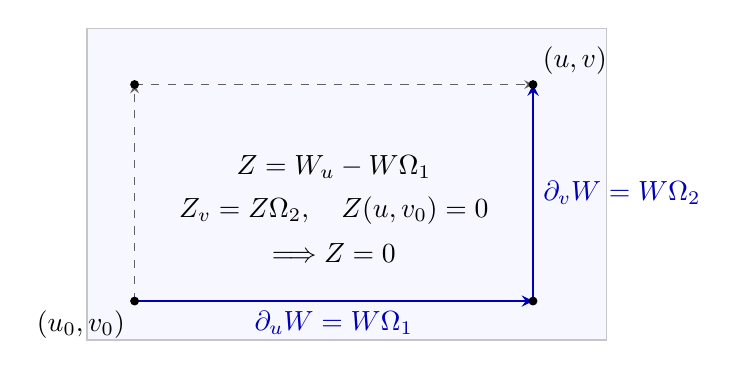
\begin{tikzpicture}[x=1.1cm,y=1.1cm,>=stealth]
	\fill[blue!3] (-0.55,-0.45) rectangle (5.45,3.15);
	\draw[gray!45] (-0.55,-0.45) rectangle (5.45,3.15);
	\draw[->,thick,blue!70!black] (0,0)--node[below] {\(\partial_uW=W\Omega_1\)} (4.6,0);
	\draw[->,thick,blue!70!black] (4.6,0)--node[right] {\(\partial_vW=W\Omega_2\)} (4.6,2.5);
	\draw[->,dashed,gray!75!black] (0,0)--(0,2.5);
	\draw[->,dashed,gray!75!black] (0,2.5)--(4.6,2.5);
	\fill (0,0) circle (1.6pt) node[below left] {\((u_0,v_0)\)};
	\fill (4.6,0) circle (1.6pt);
	\fill (0,2.5) circle (1.6pt);
	\fill (4.6,2.5) circle (1.6pt) node[above right] {\((u,v)\)};
	\node at (2.3,1.55) {\(Z=W_u-W\Omega_1\)};
	\node at (2.3,1.05) {\(Z_v=Z\Omega_2,\quad Z(u,v_0)=0\)};
	\node at (2.3,0.55) {\(\Longrightarrow Z=0\)};
\end{tikzpicture}

	\caption[矩形上的标架积分]{先沿水平线积分，再沿竖线积分。平坦性使横向误差 \(Z\) 始终为零，故交换这两个积分方向也得到同一终点标架。}
	\label{g1:fig:surface-rectangle-integration}
\end{figure}

\subsection{从标架到闭的向量值一形式}
\label{g1:subsec:0804:04}

现在假定给定数据满足 Gauss–Codazzi 条件，在任意包含基点 \(q_0=(u_0,v_0)\) 的矩形 \(V\subseteq U\) 上，用\cref{g1:lem:rectangular-matrix-system}解出初值 \(W_0\in \operatorname{SO}(3)\) 的正交标架 \(W\)，再令
\[
	\mathcal F=WP=(a_1,a_2,n).
\]
由\eqref{g1:eq:surface-orthonormal-frame-system}的定义，
\[
	\partial_i\mathcal F
	=W\Omega_iP+W\partial_iP
	=WPA_i=\mathcal F A_i.
\]
所以 \(a_1,a_2\) 已有了候选切向量应有的导数关系。还欠位置函数 \(X\)：必须证明这两个向量确实能同时写成 \(X_u,X_v\)。

\ProseParagraphBreak

把候选微分写作
\[
	\alpha=a_1\,\mathrm{d}u+a_2\,\mathrm{d}v.
\]
这是一个\term[xiangliangzhiyixingshi]{向量值一形式}[vector-valued 1-form]；这里，它将参数平面中的位移 \((\xi^1,\xi^2)\) 送到向量 \(a_1\xi^1+a_2\xi^2\)。若它的每个实分量都满足混合偏导条件，就称它为闭的；该条件写作
\[
	\mathrm{d}\alpha=(\partial_u a_2-\partial_v a_1)\,\mathrm{d}u\wedge \mathrm{d}v=0.
\]
这里 \(\mathrm{d}u\wedge \mathrm{d}v\) 只记录两个方向交换时变号；不需要预先掌握微分形式的一般理论。由 \(\partial_i\mathcal F=\mathcal F A_i\) 的前两列，
\[
	\partial_u a_2-\partial_v a_1
	=(\Gamma^1_{12}-\Gamma^1_{21})a_1
	+(\Gamma^2_{12}-\Gamma^2_{21})a_2+(h_{12}-h_{21})n=0.
\]
这一步说明了两种对称性的不同职责：Gauss–Codazzi 条件先使标架能够积分，而 \(\Gamma^k_{12}=\Gamma^k_{21}\)、\(h_{12}=h_{21}\) 再使位置的候选微分闭合。两步缺一不可。

\subsection{浸入的构造和秩检验}
\label{g1:subsec:0804:05}

在矩形上，把闭的向量值一形式积分成位置无需调用另一个一般存在定理。指定 \(x_0\in\mathbb R^3\)，直接沿刚才的折线定义
\begin{equation}
	\label{g1:eq:surface-position-rectangle-integral}
	X(u,v)=x_0+\int_{u_0}^u a_1(s,v_0)\,\mathrm{d}s+\int_{v_0}^v a_2(u,t)\,\mathrm{d}t.
\end{equation}
对 \(v\) 求导得到 \(X_v=a_2\)。对 \(u\) 求导，并用 \(\partial_u a_2=\partial_v a_1\)，得到
\[
	X_u=a_1(u,v_0)+\int_{v_0}^v\partial_u a_2(u,t)\,\mathrm{d}t
	=a_1(u,v_0)+a_1(u,v)-a_1(u,v_0)=a_1(u,v).
\]
于是 \(\mathrm{d}X=\alpha\)，且 \(X(q_0)=x_0\)。积分中各函数光滑，故 \(X\) 光滑。

\ProseParagraphBreak

有了位置函数还不能直接宣布它是正则曲面，必须检查两个切向量处处独立。由 \(W^{\mathsf T}W=I\) 及 \(P^{\mathsf T}P=\mathcal G\)，对任意 \(\xi=(\xi^1,\xi^2)\in\mathbb R^2\)，
\[
	\|\mathrm{d}X(\xi)\|^2
	=\|a_1\xi^1+a_2\xi^2\|^2
	=g_{ij}\xi^i\xi^j.
\]
当 \(\xi\ne0\) 时，正定性使右端严格为正，因此 \(\mathrm{d}X\) 的核为零、秩为 \(2\)。这正是最初坚持 \(g\) 正定的原因；若它退化，即使所有偏导相容，也不能保证得到浸入。

\subsection{两基本形式的恢复}
\label{g1:subsec:0804:06}

构造出了浸入，还须核对它实现的是原先的数据。第一基本形式由 \(\mathcal F^{\mathsf T}\mathcal F=\mathcal G\) 立即得到：
\[
	\langle X_i,X_j\rangle=\langle a_i,a_j\rangle=g_{ij}.
\]
从\eqref{g1:eq:surface-metric-factor}的列向量关系得到
\[
	X_u\times X_v=a_1\times a_2=\sqrt D\,n,
\]
故标架第三列确实等于按参数顺序选择的单位法向 \((X_u\times X_v)/\|X_u\times X_v\|\)。取 \(\partial_i\mathcal F=\mathcal F A_i\) 的第 \(j\) 列，
\[
	X_{ij}=\Gamma^1_{ij}X_u+\Gamma^2_{ij}X_v+h_{ij}n.
\]
与 \(n\) 作内积即得 \(\langle X_{ij},n\rangle=h_{ij}\)，所以第二基本形式也恢复了。特别地，第二基本形式的符号并非由事后任取法向决定；构造中的 \(P\) 和 \(W\in \operatorname{SO}(3)\) 已使它与给定参数方向一致。

\begin{example}[平直度量配上非零弯曲]
	\label{g1:exm:fundamental-cylinder-data}
	取 \(g=\mathrm{d}u^2+\mathrm{d}v^2\)、\(h=\lambda\,\mathrm{d}u^2\)，其中 \(\lambda\ne0\) 为常数。此时 \(\Gamma=0\)、\(K_g=0\)、\(\det h=0\)，Codazzi 条件也因系数常数而成立。取 \(P=I\)、\(W(0,0)=I\)，系统成为
	\[
		A_1=\begin{pmatrix}0&0&-\lambda\\0&0&0\\\lambda&0&0\end{pmatrix},
		\qquad A_2=0.
	\]
	于是
	\[
		a_1=(\cos\lambda u,0,\sin\lambda u),\quad
		a_2=(0,1,0),\quad n=(-\sin\lambda u,0,\cos\lambda u).
	\]
	以 \(X(0,0)=0\) 积分，得到
	\[
		X(u,v)=\left(\frac{\sin\lambda u}{\lambda},\,v,\,
		\frac{1-\cos\lambda u}{\lambda}\right).
	\]
	这是半径 \(1/|\lambda|\) 的圆柱面参数化。平直的长度数据允许一个切向方向发生弯曲；Gauss 方程只要求两个主曲率的乘积为零，并不要求每个主曲率都为零。
\end{example}

\subsection{局部唯一性与整体单值}
\label{g1:subsec:0804:07}

现在把构造和唯一性合并成完整结论。初始标架所规定的是两个切向量按顺序正交归一化后的方向，而不是任意指定 \(X_u,X_v\) 的长度；后者已由 \(g\) 给定。

\begin{theorem}[曲面基本定理]
	\label{g1:thm:surface-fundamental}
	设 \(U\subseteq\mathbb R^2\) 为开集，\(g=(g_{ij})\) 为光滑正定对称矩阵，\(h=(h_{ij})\) 为光滑对称矩阵，各矩阵均为 \(2\times2\)。令 \((g^{ij})=g^{-1}\)，\(\Gamma\) 为 \(g\) 的 Christoffel 系数，\(\nabla_i\partial_j=\Gamma^k_{ij}\partial_k\)，\(R\) 为该联络的曲率，约定 \(R(V,W)Z=\nabla_V\nabla_WZ-\nabla_W\nabla_VZ-\nabla_{[V,W]}Z\)。以 \(R(\partial_1,\partial_2)\partial_j=R^k{}_{j12}\partial_k\) 定义分量，令 \(h_i{}^k=g^{k\ell}h_{i\ell}\)、\(\nabla_i h_{jk}=\partial_i h_{jk}-\Gamma^\ell_{ij}h_{\ell k}-\Gamma^\ell_{ik}h_{j\ell}\)，要求 \(R^k{}_{j12}=h_1{}^kh_{2j}-h_2{}^kh_{1j}\) 及 \(\nabla_1h_{2j}=\nabla_2h_{1j}\) 对 \(j,k=1,2\) 成立，即\eqref{g1:eq:surface-data-gauss}、\eqref{g1:eq:surface-data-codazzi}。令 \(E=g_{11}\)、\(F=g_{12}\)、\(D=\det g\)，并令 \(P=\begin{psmallmatrix}\sqrt E&F/\sqrt E&0\\0&\sqrt D/\sqrt E&0\\0&0&1\end{psmallmatrix}\)。给定 \(q_0=(u_0,v_0)\in U\)、\(x_0\in\mathbb R^3\) 及右手正交标架矩阵 \(W_0\in\operatorname{SO}(3)\)，则在每个含 \(q_0\) 的开矩形 \(V\subseteq U\) 上，存在唯一的光滑浸入 \(X\colon V\rightarrow\mathbb R^3\)，其第一、第二基本形式分别为 \(g,h\)，且
	\[
		X(q_0)=x_0,\qquad
		(X_u,X_v,n)(q_0)=W_0P(q_0),\qquad
		n=\frac{X_u\times X_v}{\|X_u\times X_v\|}.
	\]
	这里 \(P\) 由\eqref{g1:eq:surface-metric-factor}确定。若不指定这些初值，同一矩形上的任意两个这样的浸入满足
	\[
		\widetilde X=QX+b,\qquad Q\in \operatorname{SO}(3),\quad b\in\mathbb R^3.
	\]
	这一结论称为\term[qumianjibendingli]{曲面基本定理}[fundamental theorem of surface theory]。
\end{theorem}

\begin{proof}
	由\cref{g1:prop:surface-data-flatness}及\eqref{g1:eq:surface-flatness-change-frame}，\(\Omega_1,\Omega_2\) 满足平坦性；它们的斜对称性已由\eqref{g1:eq:surface-matrix-metric-compatibility}证明。\cref{g1:lem:rectangular-matrix-system}给出初值为 \(W_0\) 的 \(\operatorname{SO}(3)\) 值解。于是前面三小节的构造依次给出闭的候选微分、\eqref{g1:eq:surface-position-rectangle-integral}中的光滑浸入，以及其基本形式和法向的逐项核验，这证明存在性。

	对于任意另一个具有相同数据的浸入 \(\widetilde X\)，\cref{g1:prop:gauss-weingarten}使其坐标标架 \(\widetilde{\mathcal F}=(\widetilde X_u,\widetilde X_v,\widetilde n)\) 满足相同的 \(\partial_i\widetilde{\mathcal F}=\widetilde{\mathcal F}A_i\)。因 \(g\) 相同，\(\widetilde W=\widetilde{\mathcal F}P^{-1}\) 满足同一正交标架系统。若初值也相同，矩形积分引理的唯一性给出 \(\widetilde W=W\)，从而 \(\mathrm{d}\widetilde X=\mathrm{d}X\)。两者之差的两个偏导都为零，沿水平、竖直线段积分可知其在矩形上为常数；基点位置相同便使这个常数为零。

	若不指定初值，令 \(Q=\widetilde W(q_0)W(q_0)^{\mathsf T}\in \operatorname{SO}(3)\)。矩阵 \(QW\) 满足与 \(\widetilde W\) 相同的系统和初值，因此 \(\widetilde W=QW\)。于是 \(\mathrm{d}\widetilde X=Q\,\mathrm{d}X\)，积分得到 \(\widetilde X=QX+b\)，其中 \(b=\widetilde X(q_0)-QX(q_0)\)。
\end{proof}

这里的“唯一”保留了参数点之间的对应；若允许重新参数化，就必须同时按该坐标变换拉回 \(g,h\)。此外，保向刚性变换的限定与法向约定有关：若用一个行列式为 \(-1\) 的正交矩阵反射曲面，按参数叉积重新选择的法向会多出一个负号，第二基本形式随之变号。

\ProseParagraphBreak

对一般开集，定理保证每点附近的局部实现。若沿一条道路继续这些局部解，相交处可用同一位置和标架初值保证它们一致；每一段有限道路只需有限多个小矩形。但绕环路回来时，标架可能已经转动，或者标架虽回到原值，位置却发生平移。这与\cref{g1:prop:periodic-curve-closure}中“标架回到初值”和“位移积分为零”两个条件的区别相同。以下两个例子直接显示这两种障碍，而不把局部存在性误当成任意区域上的单值存在性。

\begin{example}[转动障碍与位移障碍]
	\label{g1:exm:surface-monodromy-obstructions}
	在环带 \(A=\{(x,y):1<\sqrt{x^2+y^2}<2\}\) 上，写 \(r=\sqrt{x^2+y^2}\)。角度 \(\theta\) 不是整个环带上的单值实函数，但
	\[
		\mathrm{d}r=\frac{x\,\mathrm{d}x+y\,\mathrm{d}y}{r},\qquad
		\mathrm{d}\theta=\frac{-y\,\mathrm{d}x+x\,\mathrm{d}y}{r^2}
	\]
	都是单值的一形式；局部选定角度后，它们就是通常的坐标微分。

	先取 \(g=\mathrm{d}r^2+c^2r^2\mathrm{d}\theta^2\)、\(h=0\)，其中 \(c>0\)。在展开角度的矩形 \((1,2)\times\mathbb R\) 上，
	\[
		\widetilde X(r,\theta)=(r\cos c\theta,r\sin c\theta,0)
	\]
	实现这两组数据，因而各局部坐标中的 Gauss–Codazzi 条件都成立。它的单位径向、角向标架绕一周后旋转 \(2\pi c\)。若 \(c\notin\mathbb Z\)，这个标架不能在 \(\theta\) 与 \(\theta+2\pi\) 处匹配。假如环带上有实现数据的单值浸入，把它写到展开角度的矩形上，再用曲面基本定理的唯一性，它必与 \(\widetilde X\) 相差固定保向刚性变换；但固定刚性变换不能消除标架的不匹配，故这样的浸入不存在。

	再取 \(g=\mathrm{d}r^2+\mathrm{d}\theta^2\)、\(h=0\)。在展开角度的矩形上，\(\widetilde X(r,\theta)=(r,\theta,0)\) 实现数据，沿径向、角向的标架都是常向量，已经没有转动障碍。然而候选位置微分为 \(\alpha=(\mathrm{d}r,\mathrm{d}\theta,0)\)，沿任一正向圆周积分得到
	\[
		\oint\alpha=(0,2\pi,0)\ne0.
	\]
	一个单值位置函数的微分沿环路积分必须等于终点减起点，即零；这里却存在非零位移。也可直接由 \(\widetilde X(r,\theta+2\pi)-\widetilde X(r,\theta)=(0,2\pi,0)\) 和同样的唯一性论证排除整体浸入。
\end{example}

这两个例子中的数据处处光滑并且满足相容方程，障碍只在绕环带一周后出现。因而 Gauss–Codazzi 方程精确回答了局部能否实现的问题；在带孔区域上还要另查标架运输和环路位移，不能仅检查点上的曲率等式。

% !TeX root = ../../Book1.tex
% 纲要标题：### 8.5 模型、形变与刚性的界线
% 纲要位置：几何学计划纲要.md，第 453 行。
% 正文状态：初稿；尚未正式审核。

% 纲要内容开始
% 
% * 球面、圆柱和旋转曲面的核验
% * 平面与圆柱的局部等距
% * 一阶、局部和整体刚性问题的区分
% 
% ---
% 
% 纲要内容结束

\section{模型、形变与刚性的界线}
\label{g1:sec:0805}

曲面基本定理需要同时给定 \(I\) 和 \(II\)。如果只给 \(I\)，内在曲率虽然已经确定，两个主曲率及曲面在空间中的形状却还可能变化。本节把这种自由算在几个熟悉模型上，再区分三个常被混在一起的问题：一个变动在一阶上是否保持度量，是否存在真实的等距形变，以及局部构造能否在整张曲面上成立。

\subsection{球面、圆柱和旋转曲面的核验}
\label{g1:subsec:0805:01}

\begin{example}[球面与法向的符号]\label{g1:exm:sphere-two-forms}
	半径 \(R>0\) 的球面去掉两极后，可在经度的局部区间中用
	\[
		X(s,\theta)=\bigl(R\sin(s/R)\cos\theta,\ R\sin(s/R)\sin\theta,\ R\cos(s/R)\bigr),
		\quad 0<s<\pi R
	\]
	参数化。直接求导得到
	\[
		I=\mathrm{d}s^2+R^2\sin^2(s/R)\,\mathrm{d}\theta^2,\qquad
		n=\frac{X}{R}=\frac{X_s\times X_\theta}{\|X_s\times X_\theta\|}.
	\]
	因为 \(\mathrm{d}n=\mathrm{d}X/R\)，本书约定 \(S=-\mathrm{d}n\) 给出 \(S=-R^{-1}\operatorname{id}\)，所以
	\[
		II=-R^{-1}I,\qquad k_1=k_2=-R^{-1},\qquad H=-R^{-1},\qquad K=R^{-2}.
	\]
	因此标准球面仍有正的 Gauss 曲率；外向法向下主曲率为负，与 \(S=-\mathrm{d}n\) 一致。反向选择法向时 \(II,H,k_1,k_2\) 改号，\(I,K\) 不变。参数在两极退化，因为 \(X_\theta=0\)，但球面本身在那里可以改用图像坐标，没有几何奇点。
\end{example}

\begin{example}[圆柱的两个方向]\label{g1:exm:cylinder-two-forms}
	取
	\[
		C(u,v)=\bigl(R\cos(u/R),R\sin(u/R),v\bigr),\qquad R>0.
	\]
	有 \(C_u=(-\sin(u/R),\cos(u/R),0)\)、\(C_v=(0,0,1)\)，两者单位且正交。外向法向 \(n=(\cos(u/R),\sin(u/R),0)\) 等于 \(C_u\times C_v\)，而
	\[
		n_u=R^{-1}C_u,\qquad n_v=0.
	\]
	故
	\[
		I=\mathrm{d}u^2+\mathrm{d}v^2,\qquad II=-R^{-1}\mathrm{d}u^2,\qquad
		k_1=-R^{-1},\quad k_2=0,\quad H=-\frac1{2R},\quad K=0.
	\]
	圆周方向发生弯曲，母线方向没有法向弯曲。这里有一个零主曲率并不表示整张曲面是平面，也不表示参数不正则。
\end{example}

这两例都可由旋转曲面的统一公式找回。取光滑单位速率平面曲线 \((r(s),z(s))\)，假设 \(r>0\) 且 \(r'^2+z'^2=1\)，绕 \(z\) 轴旋转：
\[
	X(s,\theta)=(r(s)\cos\theta,r(s)\sin\theta,z(s)).
\]
弧长条件只作用于母线；\(\theta\) 方向的长度因子仍为 \(r\)。

\begin{proposition}[旋转曲面的基本形式]\label{g1:prop:revolution-two-forms}
	在上述光滑单位速率母线、\(r>0\) 及局部角参数条件下，选择法向
	\[
		n=(-z'\cos\theta,-z'\sin\theta,r'),
	\]
	则
	\[
		I=\mathrm{d}s^2+r^2\mathrm{d}\theta^2,\qquad
		II=(r'z''-z'r'')\,\mathrm{d}s^2+rz'\,\mathrm{d}\theta^2.
	\]
	子午线和纬线方向为主方向，主曲率及 Gauss 曲率为
	\begin{equation}\label{g1:eq:revolution-curvatures}
		k_s=r'z''-z'r'',\qquad k_\theta=\frac{z'}r,\qquad
		K=-\frac{r''}r,\qquad H=\frac12\left(r'z''-z'r''+\frac{z'}r\right).
	\end{equation}
	在脐点，这两方向仍是主方向，但不再是仅有的主方向。
\end{proposition}

\begin{proof}
	计算 \(X_s,X_\theta\) 得到 \(\|X_s\|=1\)、\(\|X_\theta\|=r\)、\(\langle X_s,X_\theta\rangle=0\)，且 \(X_s\times X_\theta=rn\)。二阶导数与 \(n\) 的内积分别是
	\[
		\langle X_{ss},n\rangle=-z'r''+r'z'',\qquad
		\langle X_{s\theta},n\rangle=0,\qquad
		\langle X_{\theta\theta},n\rangle=rz'.
	\]
	因此 \(I,II\) 都对角，形算子的两个特征值是相应对角项之比。最后，由单位速率条件求导得 \(r'r''+z'z''=0\)，从而
	\[
		z'(r'z''-z'r'')=-r'^2r''-z'^2r''=-r'',
	\]
	即得 \(K=-r''/r\)。此推导没有除以 \(z'\)，故 \(z'=0\) 的点也包括在内。
\end{proof}

令 \(r=R\sin(s/R),z=R\cos(s/R)\)，就得到外向球面的两个负主曲率。令 \(r=R,z=s\)，则上面指定的法向朝向圆柱轴线，因而 \(k_\theta=1/R\)；它与前一例的负号差别完全来自法向，不能直接混用。对圆锥的去顶点部分，取 \(r=as,z=bs\)，其中 \(s>0,a>0,a^2+b^2=1\)，可得 \(K=0\)。\(r=0\) 的顶点不属于命题的适用区域，零曲率公式不能被延伸为顶点正则性的证明。

\begin{example}[一个非平面的负曲率模型]\label{g1:exm:catenoid-curvatures}
	取 \(r(s)=\sqrt{a^2+s^2}\)、\(z(s)=a\,\operatorname{arsinh}(s/a)\)，其中 \(a>0\)。这里 \(\operatorname{arsinh}\) 是双曲正弦的反函数，导数为 \(1/\sqrt{1+t^2}\)。计算得
	\[
		r'=\frac{s}{r},\quad z'=\frac ar,\quad
		r''=\frac{a^2}{r^3},\quad z''=-\frac{as}{r^3}.
	\]
	因此母线确实单位速率，而旋转曲面的 \(k_s=-a/r^2\)、\(k_\theta=a/r^2\)，故 \(H=0\)、\(K=-a^2/r^4<0\)。这是\term[xuanlianmian]{悬链面}[catenoid]的一个弧长参数表示。平均曲率为零表示两个带符号主曲率相互抵消，绝不是两个主曲率都为零。
\end{example}

\subsection{平面与圆柱的局部等距}
\label{g1:subsec:0805:02}

平面 \(P(u,v)=(u,v,0)\) 与圆柱参数 \(C(u,v)\) 的第一基本形式都为 \(\mathrm{d}u^2+\mathrm{d}v^2\)。在宽度小于 \(2\pi R\) 的开条带上，\(C\) 单射，故对应 \(P(u,v)\mapsto C(u,v)\) 是局部曲面之间的等距。由\cref{g1:prop:local-isometry-length}，任意纸上曲线的长度以及相交角度都保持；这正是“无拉伸卷起”的数学含义。

\ProseParagraphBreak

它不可能由空间刚性运动得到：平面的第二基本形式恒为零，而圆柱的第二基本形式不为零；刚性运动保持第二基本形式（同时推送所选法向），反射至多因法向约定带来整体改号，也不能把零变成非零。第一基本形式的相同因此不足以触发上一节的曲面唯一性结论。

\begin{example}[从平面连续卷起]\label{g1:exm:plane-cylinder-bending}
	在固定有界矩形 \(U=(-a,a)\times(-b,b)\) 上定义
	\[
		X_t(u,v)=
		\begin{cases}
			\bigl(\sin(tu)/t,\ v,\ (1-\cos(tu))/t\bigr),&t\ne0,\\
			(u,v,0),&t=0.
		\end{cases}
	\]
	函数 \(\sin(tu)/t=\int_0^u\cos(t\xi)\,\mathrm{d}\xi\)、\((1-\cos(tu))/t=\int_0^u\sin(t\xi)\,\mathrm{d}\xi\) 表明 \(X_t\) 对 \((t,u,v)\) 光滑，并无真实的 \(t=0\) 奇点。因为
	\[
		(X_t)_u=(\cos(tu),0,\sin(tu)),\qquad (X_t)_v=(0,1,0),
	\]
	全部 \(t\) 对应的第一基本形式都为 \(\mathrm{d}u^2+\mathrm{d}v^2\)。取 \(n_t=(-\sin(tu),0,\cos(tu))\)，则 \(II_t=t\,\mathrm{d}u^2\)。当 \(|t|a<\pi/2\) 时第一坐标对 \(u\) 严格递增，故每个 \(X_t\) 还是嵌入。这个例子既给出真实的局部等距形变，又清楚显示被改变的数据是第二基本形式。
\end{example}

\cref{g1:fig:plane-cylinder-bending}画出同一参数网格在 \(t=0\) 与 \(t=1\) 时的样子。网格线在图纸上的投影长度可以不同；被保持的是曲面自身的 \(I\)，并非观看图像时的平面投影距离。

% !TeX root = ../Book1.tex
\begin{figure}[htbp]
	\centering
	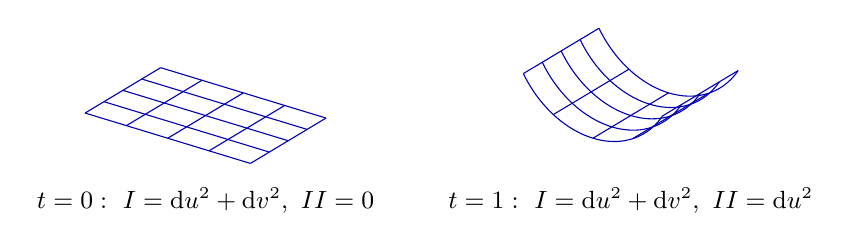
\begin{tikzpicture}[x={(1.05cm,-0.32cm)},y={(0.6cm,0.36cm)},z={(0cm,1.2cm)},font=\small]
		\begin{scope}[xshift=-2.8cm]
			\foreach \a in {-1,-0.5,0,0.5,1}{\draw[blue!70!black] (\a,-0.8,0)--(\a,0.8,0);}
			\foreach \b in {-0.8,-0.4,0,0.4,0.8}{\draw[blue!70!black] (-1,\b,0)--(1,\b,0);}
			\node at (0,0,-0.9) {\(t=0:\ I=\mathrm{d}u^2+\mathrm{d}v^2,\ II=0\)};
		\end{scope}
		\begin{scope}[xshift=2.6cm]
			\foreach \a in {-1,-0.5,0,0.5,1}{\draw[blue!70!black] ({sin(deg(\a))},-0.8,{1-cos(deg(\a))})--({sin(deg(\a))},0.8,{1-cos(deg(\a))});}
			\foreach \b in {-0.8,-0.4,0,0.4,0.8}{\draw[blue!70!black,domain=-1:1,samples=41,variable=\a] plot ({sin(deg(\a))},\b,{1-cos(deg(\a))});}
			\node at (0,0,-0.9) {\(t=1:\ I=\mathrm{d}u^2+\mathrm{d}v^2,\ II=\mathrm{d}u^2\)};
		\end{scope}
	\end{tikzpicture}
	\caption[平面卷成圆柱片]{同一参数网格的等距形变。两图的第一基本形式相同；弯曲后沿 \(u\) 方向的法向随位置改变，第二基本形式随之改变。图中采用例中的法向约定。}
	\label{g1:fig:plane-cylinder-bending}
\end{figure}


如果在整个参数平面上使用 \(C\)，则 \(C(u+2\pi R,v)=C(u,v)\)。它仍逐点保持度量，却不再单射，因而不是平面到整张圆柱的等距。更强地，平面与整张圆柱之间不存在任何整体微分同胚：平面可收缩，而圆柱投影到圆周的映射与固定高度的圆周包含互为收缩关系，绕轴一周的道路不可能收缩成点。后一断言可直接由\cref{g1:thm:circle-fundamental}中 \(\pi_1(S^1)\cong\mathbb Z\) 及投影、包含的复合为恒等得到。这个拓扑障碍与局部度量计算并不矛盾。

\subsection{一阶、局部和整体刚性问题的区分}
\label{g1:subsec:0805:03}

“刚性”必须说明保持什么、在哪个区域比较以及是否允许改变参数。曲面基本定理的唯一性固定了参数域上的两种形式：若两个浸入的 \(I,II\) 相同，才比较它们是否由一个固定的空间刚性运动联系。若给定一个参数对应 \(\phi\)，应先将第二个浸入换成 \(\widetilde X\circ\phi\)，再逐项比较两种形式。

\begin{definition}[无穷小等距变动]\label{g1:def:infinitesimal-bending}
	设 \(X:U\rightarrow\mathbb R^3\) 为光滑浸入，\(V:U\rightarrow\mathbb R^3\) 为沿 \(X\) 的光滑向量场。若
	\begin{equation}\label{g1:eq:infinitesimal-bending}
		\langle\partial_iV,X_j\rangle+\langle X_i,\partial_jV\rangle=0,\qquad i,j=1,2,
	\end{equation}
	称 \(V\) 为一个\term[wuqiongxiaodengjubiandong]{无穷小等距变动}[infinitesimal bending]。若 \(V=a+\Omega X\)，其中 \(a\in\mathbb R^3\) 固定、\(\Omega\) 为固定斜对称矩阵，称其为刚性运动产生的变动。
\end{definition}

几何上 \(V(q)\) 是曲面点最初的移动速度。若光滑族 \(X_t\) 满足 \(X_0=X\)，则对 \(g_{ij}(t)=\langle(X_t)_i,(X_t)_j\rangle\) 求 \(t\) 导数，正好得到\eqref{g1:eq:infinitesimal-bending}，其中 \(V=\partial_tX_t|_{t=0}\)。因此真正的等距形变一定产生无穷小等距变动。斜对称矩阵给出
\[
	\langle\Omega X_i,X_j\rangle+\langle X_i,\Omega X_j\rangle=0,
\]
所以刚性运动产生的变动总满足这个线性方程。

\begin{example}[一阶条件并不足够]\label{g1:exm:nonintegrable-plane-bending}
	对平面 \(X(u,v)=(u,v,0)\)，任意光滑函数 \(f\) 都给出 \(V=f(u,v)(0,0,1)\)，并满足\eqref{g1:eq:infinitesimal-bending}，因为 \(\partial_iV\) 总与平面垂直。它不一定来自真正的等距形变。取 \(f=u^2+v^2\)，假设有对 \((t,u,v)\) 光滑的浸入族 \(X_t\)，使 \(X_0=X\)、\(\partial_tX_t|_0=V\)，且 \(I_t=\mathrm{d}u^2+\mathrm{d}v^2\)。取由参数定向决定的法向 \(n_t\)。因为 \(X_{ij}|_{t=0}=0\)，
	\[
		h_{ij}(0)=0,\qquad
		\left.\partial_t h_{ij}(t)\right|_0
		=\langle\partial_i\partial_jV,(0,0,1)\rangle=f_{ij}.
	\]
	因此在任一固定参数点有 \(h(t)=2tI_2+O(t^2)\)，从而 \(\det h(t)=4t^2+O(t^3)\)。可是固定的平面度量具有 \(K=0\)，由\cref{g1:thm:gauss-equation}必须有 \(\det h(t)=K\det g=0\)，矛盾。这里一阶约束全满足，二阶相容性却阻止了真实形变。
\end{example}

相比之下，\cref{g1:exm:plane-cylinder-bending}在 \(t=0\) 的变动为 \(V=(u^2/2)(0,0,1)\)，它确实来自整个等距族；其二阶导数矩阵的行列式为零。这个比较只说明上述必要障碍在后一例中消失，不能反过来把“行列式为零”未经证明地宣布为任意形变都可积分的充分条件。

\begin{proposition}[两种形式相同的整体唯一性]\label{g1:prop:surface-global-uniqueness}
	设 \(U\subseteq\mathbb R^2\) 为连通开集，\(X,\widetilde X:U\rightarrow\mathbb R^3\) 为光滑浸入，均取参数定向的单位法向。若两者在同一参数下具有相同的第一、第二基本形式，则存在一个固定 \(Q\in \operatorname{SO}(3)\) 和 \(a\in\mathbb R^3\)，使 \(\widetilde X=QX+a\) 在整个 \(U\) 上成立。这里不要求 \(U\) 单连通。
\end{proposition}

\begin{proof}
	在一点由两组标架与位置确定 \(Q,a\)，再将 \(\widetilde X\) 替换为 \(Q^{-1}(\widetilde X-a)\)。设两者的位置、两个一阶偏导及法向全部相同的点集为 \(A\)。这个集合非空，由连续性为闭集。每个 \(q\in A\) 都有一个矩形邻域；\cref{g1:thm:surface-fundamental}中指定位置及标架初值的唯一性使两浸入在该矩形内相同，所以 \(A\) 也开。连通性给出 \(A=U\)。只比较已经存在的两个整体解时，不会发生“沿不同道路构造出不同解”的问题，因此无需用单连通性排除运输障碍。
\end{proof}

由此可见，局部存在、整体存在与整体唯一性有不同的条件。相容性给出小邻域上的实现；绕闭路运输能否回到同一标架和同一位置，决定能否将局部实现接成单值的整体实现；两个已经存在的实现若保持全部数据，其唯一性又可由连通性传播。本章没有把仅保持第一基本形式的闭曲面刚性问题归结为这一命题。


\begin{chaptersummary}
	浸入要求两个参数方向在空间中仍然独立，它只保证局部图像模型。第一基本形式是切向量的内积，按坐标换元公式转换；长度、面积、梯度、散度与 Laplace 算子由它确定。参数矩阵的样子可以改变，而内积及其测量含义不改变。局部等距保持这套数据，却可能改变曲面在空间中的形状。

	\ProseParagraphBreak

	固定法向以后，形算子 \(S=-\mathrm{d}n\) 和第二基本形式记录法向弯曲。自伴性给出正交主方向，Euler 公式把任意方向的法曲率写成两个主曲率的加权平均。平均曲率与 Gauss 曲率分别是半迹与行列式；法向反转使前者改号，却不改变后者。脐点、零主曲率和渐近方向的退化须逐项区分，不能从一个点的二阶数据直接推出邻域的形状。

	\ProseParagraphBreak

	结构方程把坐标标架的导数分为切向与法向两部分。协变导数记录切向变化，其系数由度量决定；混合偏导相容性同时给出 Gauss 与 Codazzi 方程。Gauss 方程使两个主曲率的乘积成为内在量，这解释了球面不能局部等距铺平，也解释了平面和圆柱虽有相同的零 Gauss 曲率，仍可有不同的主曲率。

	\ProseParagraphBreak

	反向构造先把给定度量分解为标架的长度约束，再把相容条件转为矩阵系统的平坦性。两次普通微分方程积分、误差的零初值唯一性，以及闭向量值一形式的显式积分，共同得到局部浸入；正定性落实秩为二，列向量的内积和导数恢复全部数据。在同一参数下，两种形式共同决定曲面到保向刚性运动为止。整体单值还可能遇到转动或位移障碍，整体单射和仅保持度量的刚性则是进一步的问题。
\end{chaptersummary}

\BookExercises
以下习题均附完整解答。计算前先固定参数和法向；使用存在或唯一性结论时，区分给定的是第一基本形式、两种基本形式，还是只有它们的一阶变化。

\begin{exercise}\label{g1:ex:oblique-metric-measurements}
	对 \(X(u,v)=(u+v,v,0)\)，求参数单位正方形的面积、两条对角线的长度及函数 \(f(u,v)=u\) 的曲面梯度。说明参数分量 \((1,0)\) 为什么不是该梯度。
\end{exercise}
\begin{solution}
	度量矩阵及其逆为
	\[
		g=\begin{pmatrix}1&1\\1&2\end{pmatrix},\qquad
		g^{-1}=\begin{pmatrix}2&-1\\-1&1\end{pmatrix},\qquad D=1.
	\]
	故单位正方形的像为面积 \(1\) 的平行四边形。两条对角线的参数方向分别是 \((1,1)\) 与 \((1,-1)\)，在参数长度为 \(1\) 的区间上走过，平方速度分别为 \(5\) 与 \(1\)，所以长度为 \(\sqrt5\) 与 \(1\)。

	由\eqref{g1:eq:surface-gradient}，\(\operatorname{grad}_gf=2\partial_u-\partial_v\)，空间向量为 \(2X_u-X_v=(1,-1,0)\)。空间平面上 \(f=x-y\)，确实有这个 Euclid 梯度。如果误用 \(\partial_u\)，则它与 \(\partial_v\) 的内积是 \(g_{12}=1\)，而 \(\mathrm{d}f(\partial_v)=0\)，不满足梯度的定义。
\end{solution}

\begin{exercise}\label{g1:ex:graph-area-gradient}
	设 \(X(u,v)=(u,v,f(u,v))\) 为光滑图像，令 \(w=(f_u,f_v)^{\mathsf T}\)。
	\begin{enumerate}
		\item 证明 \(g=I_2+ww^{\mathsf T}\)，并求 \(D\)、\(g^{-1}\) 与高度函数 \(f\) 的曲面梯度。
		\item 对 \(f=(u^2+v^2)/2\)，求参数圆盘 \(u^2+v^2\le R^2\) 对应曲面片的面积。
	\end{enumerate}
\end{exercise}
\begin{solution}
	1. 由 \(X_u=(1,0,f_u),X_v=(0,1,f_v)\)，立即得到所给矩阵。展开二阶行列式，有 \(D=1+|w|^2\)。直接相乘可验
	\[
		(I_2+ww^{\mathsf T})\left(I_2-\frac{ww^{\mathsf T}}{1+|w|^2}\right)=I_2,
	\]
	所以 \(g^{-1}=I_2-ww^{\mathsf T}/(1+|w|^2)\)。于是梯度的参数分量为 \(w/(1+|w|^2)\)，对应空间向量
	\[
		\operatorname{grad}f=\frac{(f_u,f_v,f_u^2+f_v^2)}{1+f_u^2+f_v^2}.
	\]
	它也等于 \((0,0,1)-\langle(0,0,1),n\rangle n\)，其中 \(n=(-f_u,-f_v,1)/\sqrt{1+|w|^2}\)，与投影解释相符。

	2. 此时 \(D=1+u^2+v^2\)，用平面极坐标积分得
	\[
		\operatorname{Area}=2\pi\int_0^Rr\sqrt{1+r^2}\,\mathrm{d}r
		=\frac{2\pi}{3}\bigl((1+R^2)^{3/2}-1\bigr).
	\]
	被积函数中的一个 \(r\) 来自参数平面的极坐标换元，\(\sqrt{1+r^2}\) 才是图像的面积伸缩因子；两者不可遗漏或混同。
\end{solution}

\begin{exercise}\label{g1:ex:conformal-laplacian}
	在平面开集 \(U\) 上取 \(g=e^{2\phi}(\mathrm{d}u^2+\mathrm{d}v^2)\)，其中 \(\phi\) 光滑。求 \(\operatorname{grad}_gf\) 和 \(\Delta_gf\)，并证明对任意 \(f\in C_c^\infty(U)\)，积分 \(\int_U|\operatorname{grad}_gf|_g^2\,\mathrm{d}A_g\) 与 \(\phi\) 无关。由此判断，在这个度量下满足 \(\Delta_gf=0\) 的函数是否与 Euclid 度量下相同。
\end{exercise}
\begin{solution}
	这里 \(g^{ij}=e^{-2\phi}\delta_{ij}\)，\(\sqrt D=e^{2\phi}\)。因此
	\[
		\operatorname{grad}_gf=e^{-2\phi}(f_u\partial_u+f_v\partial_v),\qquad
		\Delta_gf=-e^{-2\phi}(f_{uu}+f_{vv}).
	\]
	散度中的乘积 \(\sqrt D\,g^{ij}\) 恰为 \(\delta_{ij}\)，这就是没有出现 \(\phi\) 的导数的原因。又
	\[
		|\operatorname{grad}_gf|_g^2=e^{-2\phi}(f_u^2+f_v^2),
		\qquad
		\int_U|\operatorname{grad}_gf|_g^2\,\mathrm{d}A_g
		=\int_U(f_u^2+f_v^2)\,\mathrm{d}u\,\mathrm{d}v.
	\]
	因 \(e^{-2\phi}>0\)，\(\Delta_gf=0\) 等价于 \(f_{uu}+f_{vv}=0\)，解的集合确实相同；不过算子本身和度量长度通常不同，不能因此把两个度量判为等距。
\end{solution}

\begin{exercise}\label{g1:ex:area-angle-not-isometry}
	在两个标准 Euclid 平面之间，分别考虑 \(\phi(u,v)=(2u,v/2)\) 和 \(\psi(u,v)=(2u,2v)\)。判断它们是否保持面积、是否保持夹角、是否局部等距，并为每个否定结论给出具体的方向或区域。
\end{exercise}
\begin{solution}
	\(\phi\) 的导数行列式为 \(1\)，故由面积换元保持每个区域的面积。但 \((1,0)\) 的长度从 \(1\) 变为 \(2\)，所以不是局部等距。原来正交的方向 \(a=(1,1)\)、\(b=(1,-1)\) 映为 \((2,1/2)\)、\((2,-1/2)\)，内积为 \(15/4\ne0\)，故也不保持夹角。

	\(\psi\) 把内积乘以 \(4\)，向量长度乘以 \(2\)，夹角公式中的因子抵消，故保持夹角；但单位正方形面积变成 \(4\)，单位线段长度变成 \(2\)，所以既不保持面积，也不是局部等距。单独保持面积或单独保持夹角都不足以代替第一基本形式的完整条件。
\end{solution}

\begin{exercise}\label{g1:ex:shape-oblique-basis}
	在某曲面的一点，以坐标切基 \(X_1,X_2\) 表示的两基本形式矩阵为
	\[
		g=\begin{pmatrix}2&1\\1&1\end{pmatrix},\qquad h=\begin{pmatrix}2&0\\0&-1\end{pmatrix}.
	\]
	求形算子矩阵、主曲率及一组正交单位主向量，并求沿 \(X_1,X_2\) 的法曲率。形算子矩阵不是通常的对称矩阵，为什么不违反其自伴性？
\end{exercise}
\begin{solution}
	因为 \(\det g=1\)，
	\[
		[S]=g^{-1}h=\begin{pmatrix}1&-1\\-1&2\end{pmatrix}
		\begin{pmatrix}2&0\\0&-1\end{pmatrix}
		=\begin{pmatrix}2&1\\-2&-2\end{pmatrix}.
	\]
	迹为 \(0\)，行列式为 \(-2\)，所以主曲率为 \(k_\pm=\pm\sqrt2\)。对应的特征向量可取
	\[
		w_\pm=X_1+(k_\pm-2)X_2.
	\]
	用给定的 \(g\) 而不是把系数当作直角坐标计算，得到
	\[
		\langle w_+,w_-\rangle
		=2+(k_+-2)+(k_--2)+(k_+-2)(k_--2)=0,
	\]
	且 \(\lVert w_\pm\rVert^2=2+2(k_\pm-2)+(k_\pm-2)^2=4-2k_\pm>0\)。于是 \(e_\pm=w_\pm/\sqrt{4-2k_\pm}\) 是所求正交单位主向量。

	两个坐标方向的法曲率分别为 \(h_{11}/g_{11}=1\) 和 \(h_{22}/g_{22}=-1\)，均不同于主曲率，说明坐标方向并非主方向。自伴性在这个基下应写成 \([S]^{\mathsf T}g=g[S]\)，两边都等于 \(h\)；只有 \(g=I\) 的正交单位基才把这个条件化成矩阵自身对称。
\end{solution}

\begin{exercise}\label{g1:ex:graph-mean-curvature}
	设 \(X(u,v)=(u,v,f(u,v))\) 为光滑图像，取向上法向。推导
	\[
		H=\frac{(1+f_v^2)f_{uu}-2f_uf_vf_{uv}+(1+f_u^2)f_{vv}}
		{2(1+f_u^2+f_v^2)^{3/2}},
		\qquad
		K=\frac{f_{uu}f_{vv}-f_{uv}^2}{(1+f_u^2+f_v^2)^2}.
	\]
	对 \(f(u,v)=u^2-v^2\) 求 \(H,K\)，说明一个点的 \(H=0\) 既不能直接推出整个邻域的 \(H=0\)，也不能推出曲面在该点附近为平面。
\end{exercise}
\begin{solution}
	由\cref{g1:exm:graph-second-form}，令 \(W=\sqrt{1+f_u^2+f_v^2}\)，则 \(E=1+f_u^2\)、\(F=f_uf_v\)、\(G=1+f_v^2\)、\(D=W^2\)，并有 \(h_{ij}=f_{ij}/W\)。分别代入\eqref{g1:eq:surface-HK-formulas}，分子的第二基本形式贡献一个或两个 \(W^{-1}\)，便得到题设的 \(H,K\) 公式。

	对 \(f=u^2-v^2\)，有 \(f_u=2u\)、\(f_v=-2v\)、\(f_{uu}=2\)、\(f_{vv}=-2\)、\(f_{uv}=0\)。因此
	\[
		H=\frac{4(v^2-u^2)}{(1+4u^2+4v^2)^{3/2}},\qquad
		K=\frac{-4}{(1+4u^2+4v^2)^2}.
	\]
	原点 \(H=0\)，但任意邻域都含 \(v^2\ne u^2\) 的点，故 \(H\) 在该邻域不恒为零；而 \(K<0\) 已说明此曲面不是平面。这些计算分别排除了两个推断，原点的平均曲率为零只表示两个主曲率在该点相互抵消。
\end{solution}

\begin{exercise}\label{g1:ex:helicoid-asymptotic-curves}
	先证明曲面内的任意正则直线段都是渐近线。再设 \(a>0\)，考虑
	\[
		X(u,v)=(u\cos v,u\sin v,av),\qquad u>0,\quad v\in\mathbb R.
	\]
	取 \(X_u\times X_v\) 确定的法向，求两基本形式及 \(H,K\)。证明两族坐标曲线都是渐近线，并说明其中一族不是直线，从而否定上述结论的逆命题。
\end{exercise}
\begin{solution}
	直线段改用弧长后加速度为零，由\cref{g1:prop:surface-normal-acceleration}知 \(\mathrm{II}(\gamma',\gamma')=0\)，所以是渐近线。

	对题设曲面，记 \(W=\sqrt{u^2+a^2}\)。有
	\[
		X_u=(\cos v,\sin v,0),\qquad X_v=(-u\sin v,u\cos v,a),\qquad
		n=\frac{(a\sin v,-a\cos v,u)}W.
	\]
	由 \(E=1,F=0,G=W^2\) 可知浸入处处正则。又
	\[
		X_{uu}=0,\qquad X_{uv}=(-\sin v,\cos v,0),\qquad
		X_{vv}=(-u\cos v,-u\sin v,0),
	\]
	与 \(n\) 作内积得到 \(h_{11}=h_{22}=0\)、\(h_{12}=-a/W\)。所以
	\[
		\mathrm I=(\mathrm du)^2+(u^2+a^2)(\mathrm dv)^2,\qquad
		\mathrm{II}=-\frac{2a}{W}\,\mathrm du\,\mathrm dv,\qquad
		H=0,\quad K=-\frac{a^2}{(u^2+a^2)^2}.
	\]
	因 \(a/W\ne0\)，渐近方向恰由 \(\mathrm du\,\mathrm dv=0\) 给出，故 \(u\) 固定与 \(v\) 固定的两族坐标曲线都是渐近线。固定 \(v\) 得到直线；固定 \(u=u_0>0\) 则得到圆柱螺线 \((u_0\cos v,u_0\sin v,av)\)，其曲率为 \(u_0/(u_0^2+a^2)>0\)，不是直线。这与渐近条件并不矛盾：它的加速度沿曲面的切平面，而不是沿曲面法向。
\end{solution}

\begin{exercise}\label{g1:ex:gauss-map-area-factor}
	设光滑浸入 \(X:U\to\mathbb R^3\) 取单位法向 \(n=(X_1\times X_2)/\sqrt D\)。证明
	\[
		n_1\times n_2=K(X_1\times X_2),\qquad
		\lVert n_1\times n_2\rVert=|K|\sqrt D.
	\]
	解释后一式中 \(|K|\) 的面积意义，并用图像 \(z=x^2\) 说明：\(K\) 恒为零也不能推出 Gauss 映射为常值。
\end{exercise}
\begin{solution}
	以 \(X_1,X_2\) 为基，\(n_i=-S(X_i)\)。二维线性变换对有向平行四边形的面积乘以行列式；在这里直接按两个系数展开叉积，也得到
	\[
		n_1\times n_2=(-S(X_1))\times(-S(X_2))
		=\det(-S)(X_1\times X_2)=K(X_1\times X_2).
	\]
	两边取范数，并用 \(\lVert X_1\times X_2\rVert=\sqrt D\)，即得第二式。曲面原来的面积密度为 \(\sqrt D\)，Gauss 映射在单位球面上扫过的参数面积密度为 \(\lVert n_1\times n_2\rVert\)；两者之比是 \(|K|\)。这个说法是局部的面积变化率，若不同参数点映到同一法向，参数面积积分仍会计入各次覆盖。

	对 \(X(u,v)=(u,v,u^2)\)，有
	\[
		n(u,v)=\frac{(-2u,0,1)}{\sqrt{1+4u^2}},\qquad
		h=\frac1{\sqrt{1+4u^2}}\begin{pmatrix}2&0\\0&0\end{pmatrix}.
	\]
	因 \(\det h=0\)，处处 \(K=0\)，但 \(n\) 随 \(u\) 变化。这里 Gauss 映射的微分秩为 \(1\)，所以它没有扫出二维面积，却仍扫过一条球面曲线。行列式为零只表示面积塌缩，并不表示整个微分为零。
\end{solution}


\begin{exercise}\label{g1:ex:polar-parallel-vector}
	在去掉原点的平面上，令 \(e_r=(\cos\theta,\sin\theta,0)\)、\(e_\theta=(-\sin\theta,\cos\theta,0)\)。沿圆周 \(r=r_0>0\)，写切向量场 \(V(\theta)=a(\theta)e_r+b(\theta)e_\theta\)。利用本章的协变导数求出 \(\nabla_{\mathrm d/\mathrm d\theta}V=0\) 的所有解，并解释为什么分量改变而几何向量可以不变。这里沿参数曲线的协变导数指普通导数向平面切空间的投影。
\end{exercise}
\begin{solution}
	平面切空间恒定，普通导数已经是切向量。由 \(\mathrm de_r/\mathrm d\theta=e_\theta\)、\(\mathrm de_\theta/\mathrm d\theta=-e_r\)，
	\[
		\nabla_{\mathrm d/\mathrm d\theta}V
		=(\dot a-b)e_r+(\dot b+a)e_\theta.
	\]
	所以方程等价于 \(\dot a=b\)、\(\dot b=-a\)，其全部解为
	\[
		a=A\cos\theta+B\sin\theta,\qquad
		b=-A\sin\theta+B\cos\theta,
	\]
	其中 \(A,B\) 为常数。可直接代入验证，而任意初值唯一确定 \(A,B\)，也可由\cref{g1:lem:linear-frame-ode}的唯一性确认没有其他解。代回原式，得到 \(V=(A,B,0)\)，确为固定向量。变化的 \(a,b\) 只是相对于旋转基的分量；如果错误地只令 \(\dot a=\dot b=0\)，通常得到的是随圆周一起转动的向量。
\end{solution}

\begin{exercise}\label{g1:ex:two-conformal-metrics}
	\begin{enumerate}
		\item 在 \(\mathbb R^2\) 上考虑 \(g=e^{2u}(\mathrm du^2+\mathrm dv^2)\)。求它的曲率，并验证 \(X(u,v)=(e^u\cos v,e^u\sin v,0)\) 实现这个度量。这个参数化是否是到其像的整体一一对应？
		\item 在上半平面 \(v>0\) 上考虑 \(g=v^{-2}(\mathrm du^2+\mathrm dv^2)\)。求它的曲率，判断它能否局部等距于某个 Euclid 平面开集。
	\end{enumerate}
\end{exercise}
\begin{solution}
	(1) 此时 \(\phi=u\)，所以\eqref{g1:eq:conformal-gauss-curvature}给出 \(K_g=0\)。直接求导，
	\[
		X_u=e^u(\cos v,\sin v,0),\qquad
		X_v=e^u(-\sin v,\cos v,0),
	\]
	二者正交且长度均为 \(e^u\)，所以 \(X\) 是浸入并诱导所给度量。然而 \(X(u,v+2\pi)=X(u,v)\)，它不是整体一一对应。这是局部度量完全实现而参数仍有整体重复的例子。

	(2) 此时 \(\phi=-\log v\)，有 \(\phi_{uu}=0\)、\(\phi_{vv}=v^{-2}\)，故 \(K_g=-v^2\cdot v^{-2}=-1\)。Euclid 平面开集的曲率为零。若存在局部等距，重参数化后度量一致，由\cref{g1:prop:surface-curvature-two-dim}及曲率的坐标公式，曲率也应一致，矛盾。这里仅在参数域上计算给定度量，不需要先假定它在三维空间中存在整体浸入。
\end{solution}

\begin{exercise}\label{g1:ex:gauss-codazzi-independent}
	在参数域 \(U=\{(u,v):v>0\}\) 上取平坦度量 \(g=\mathrm du^2+\mathrm dv^2\)。
	\begin{enumerate}
		\item 令 \(h=v\,\mathrm du^2\)，证明它满足 Gauss 方程，但不满足 Codazzi 方程。
		\item 令 \(h=\mathrm du^2+\mathrm dv^2\)，证明它满足 Codazzi 方程，但不满足 Gauss 方程。
	\end{enumerate}
	由此判断两组数据能否作为某个曲面片的两基本形式。
\end{exercise}
\begin{solution}
	度量系数恒定，所以全部 \(\Gamma^k_{ij}=0\)，从而 \(R=0\)、\(K_g=0\)，且 \(\nabla_i h_{jk}=\partial_i h_{jk}\)。

	(1) 矩阵 \(h=\operatorname{diag}(v,0)\) 的行列式为零，故 \(K_g=\det(g^{-1}h)=0\)。由\cref{g1:prop:surface-curvature-two-dim}，这就是完整的 Gauss 方程。然而
	\[
		\nabla_1h_{21}=0,\qquad \nabla_2h_{11}=1,
	\]
	不满足 Codazzi 方程。

	(2) 矩阵 \(h=I\) 恒定，所有协变导数均为零，故 Codazzi 方程成立。但 \(\det(g^{-1}h)=1\ne0=K_g\)，Gauss 方程不成立。两组数据分别违反一个必要条件，因此均不能在任何非空开子域上作为光滑曲面片的两基本形式。
\end{solution}

\begin{exercise}\label{g1:ex:totally-umbilic-surface}
	设 \(U\subseteq\mathbb R^2\) 是连通开集，\(X\colon U\rightarrow\mathbb R^3\) 是光滑浸入，取光滑单位法向 \(n\)。假设每一点都是脐点，即 \(S=\lambda I\)，其中 \(\lambda\) 为光滑函数。证明 \(\lambda\) 为常数，并证明 \(X(U)\) 包含在某个平面或某个球面中。说明只在一个点为脐点为什么不足以得到这个结论。
\end{exercise}
\begin{solution}
	由 \(\nabla_V(\lambda W)=V(\lambda)W+\lambda\nabla_VW\)，有 \((\nabla_VS)W=V(\lambda)W\)。Codazzi 方程的形算子形式因此化为
	\[
		V(\lambda)W=W(\lambda)V.
	\]
	取 \(V=X_1,W=X_2\)，二者线性无关，故 \(\partial_1\lambda=\partial_2\lambda=0\)。函数 \(\lambda\) 在每个小圆盘内为常数，因而是局部常值函数；连通性使它在整个 \(U\) 上为同一个常数。

	若 \(\lambda=0\)，则 \(\mathrm{d}n=-S\,\mathrm{d}X=0\)，同理 \(n=n_0\) 为常向量。又 \(\partial_i\langle X,n_0\rangle=\langle X_i,n_0\rangle=0\)，所以 \(\langle X,n_0\rangle=c\)，像包含在平面内。

	若 \(\lambda\ne0\)，则
	\[
		\partial_i\left(X+\frac1\lambda n\right)
		=X_i-\frac1\lambda S X_i=0.
	\]
	故 \(X+n/\lambda=a\) 为常向量，且 \(\lVert X-a\rVert=1/|\lambda|\)，像包含在以 \(a\) 为心的球面上。这里的结论是像的包含关系，并不要求参数化整体单射。

	若只在一点有 \(S=\lambda I\)，便不能在邻域内对这个恒等式求导，Codazzi 方程也不能推出邻域中的 \(\lambda\) 为常数。例如图像 \(X(u,v)=(u,v,u^3+v^3)\) 在原点的第一导数、第二导数使 \(S(0)=0\)，原点为脐点；当 \(u=v\ne0\) 时其 Gauss 曲率为
	\[
		K(u,u)=\frac{36u^2}{(1+18u^4)^2}>0,
	\]
	而原点的曲率为零。任何包含原点的这类邻域都既不是平面片，也不可能包含在一个固定球面内，因为球面的曲率是固定的正数。
\end{solution}

\begin{exercise}
	\label{g1:ex:constant-surface-data}
	在 \(\mathbb R^2\) 上给定
	\[
		g=\mathrm{d}u^2+\mathrm{d}v^2,\qquad h=a\,\mathrm{d}u^2+2b\,\mathrm{d}u\,\mathrm{d}v+c\,\mathrm{d}v^2,
	\]
	其中 \(a,b,c\) 是实常数。确定这些数据可局部实现的充要条件，并在条件成立时给出一个定义于整个 \(\mathbb R^2\) 的实现。
\end{exercise}

\begin{solution}
	度量系数常数使 \(\Gamma=0\)、\(K_g=0\)，常数 \(h\) 自动满足 Codazzi 条件。Gauss 条件要求 \(ac-b^2=0\)，故这是必要条件。以下构造同时说明充分性。

	若 \(a=b=c=0\)，取 \(X(u,v)=(u,v,0)\)。否则对称矩阵 \(h\) 的两个特征值为 \(\lambda\ne0\) 和 \(0\)。选择单位特征向量 \(t=(t_1,t_2)\) 对应 \(\lambda\)，再取 \(q=(-t_2,t_1)\)；令 \(\xi=t_1u+t_2v\)、\(\eta=-t_2u+t_1v\)。这是保向正交坐标变换，并且 \(g=\mathrm{d}\xi^2+\mathrm{d}\eta^2\)、\(h=\lambda\,\mathrm{d}\xi^2\)。定义
	\[
		X(u,v)=\left(\frac{\sin(\lambda\xi)}{\lambda},\,\eta,\,
		\frac{1-\cos(\lambda\xi)}{\lambda}\right).
	\]
	有 \(X_\xi=(\cos\lambda\xi,0,\sin\lambda\xi)\)、\(X_\eta=(0,1,0)\)，所以第一基本形式正确；法向为 \(n=(-\sin\lambda\xi,0,\cos\lambda\xi)\)，而 \(X_{\xi\xi}=\lambda n\)、\(X_{\xi\eta}=X_{\eta\eta}=0\)，所以第二基本形式也正确。变换 \((u,v)\mapsto(\xi,\eta)\) 保向，故不会额外改变所定法向。所得浸入在整个平面上成立，但当 \(\lambda\ne0\) 时会周期性覆盖圆柱，不能据此称为嵌入。
\end{solution}

\begin{exercise}
	\label{g1:ex:simply-connected-surface-overlap}
	在整个 \(\mathbb R^2\) 上考虑数据 \(g=e^{2u}(\mathrm{d}u^2+\mathrm{d}v^2)\)、\(h=0\)。构造一个实现它们的浸入，并证明没有实现同样数据、采用参数叉积法向的单射浸入。解释这与曲面基本定理是否矛盾。
\end{exercise}

\begin{solution}
	取 \(X(u,v)=(e^u\cos v,e^u\sin v,0)\)。其偏导为
	\begin{align*}
		X_u&=e^u(\cos v,\sin v,0),\\
		X_v&=e^u(-\sin v,\cos v,0).
	\end{align*}
	内积矩阵是 \(e^{2u}I\)，叉积为 \((0,0,e^{2u})\ne0\)，所以它是所需浸入，单位法向是常向量 \((0,0,1)\)，第二基本形式为零。

	设 \(\widetilde X\) 是另一个实现。\(\mathbb R^2=\mathbb R\times\mathbb R\) 本身就是开矩形，故\cref{g1:thm:surface-fundamental}的唯一性在整个域上适用，得到 \(\widetilde X=QX+b\)。但 \(X(u,v+2\pi)=X(u,v)\)，所以 \(\widetilde X\) 同样不是单射。基本定理保证的是微分秩为二的浸入；局部点可分辨并不排除远处参数点映到同一点。这里没有整体单值障碍，只有全局单射性的失败。
\end{solution}

\begin{exercise}
	\label{g1:ex:annulus-cylinder-period}
	在环带 \(A=\{1<r<2\}\) 上给定 \(g=\mathrm{d}r^2+\mathrm{d}\theta^2\)、\(h=\lambda\,\mathrm{d}\theta^2\)，其中 \(\lambda\in\mathbb R\) 为常数，\(\mathrm{d}r,\mathrm{d}\theta\) 按\cref{g1:exm:surface-monodromy-obstructions}理解。确定哪些 \(\lambda\) 允许数据由环带上的单值浸入实现；在可以实现的情形中，判断哪些允许单射实现。
\end{exercise}

\begin{solution}
	局部坐标 \((r,\theta)\) 中 \(g,h\) 的系数都是常数，\(\Gamma=0\)，且 \(K_g=\det h=0\)，故所有 \(\lambda\) 都满足局部相容条件。在展开角度的矩形 \((1,2)\times\mathbb R\) 上，若 \(\lambda\ne0\)，取
	\[
		\widetilde X(r,\theta)=
		\left(r,\frac{\sin\lambda\theta}{\lambda},
		\frac{1-\cos\lambda\theta}{\lambda}\right).
	\]
	其偏导为 \(\widetilde X_r=(1,0,0)\)、\(\widetilde X_\theta=(0,\cos\lambda\theta,\sin\lambda\theta)\)，参数法向为 \(n=(0,-\sin\lambda\theta,\cos\lambda\theta)\)，且 \(\widetilde X_{\theta\theta}=\lambda n\)，因此实现给定数据。它在 \(\theta\mapsto\theta+2\pi\) 下为周期函数，当且仅当 \(\lambda\in\mathbb Z\)。对于 \(\lambda=0\)，实现为 \(\widetilde X=(r,\theta,0)\)，有非零的平移周期，不能下降到环带。

	任意其他实现提升到展开角度的矩形后，均由\cref{g1:thm:surface-fundamental}与上述实现相差固定保向刚性变换，故不能改变周期条件。于是恰好在 \(\lambda\in\mathbb Z\setminus\{0\}\) 时存在环带上的浸入。当 \(|\lambda|=1\) 时，第一坐标分辨 \(r\)，后两坐标分辨模 \(2\pi\) 的 \(\theta\)，所以实现单射。当 \(|\lambda|\geq2\) 时，\(\theta\) 与 \(\theta+2\pi/|\lambda|\) 在环带上是不同点，却有相同像；刚性变换也不能消除此重叠。因此单射实现恰对应 \(\lambda=\pm1\)。
\end{solution}

\begin{exercise}
	\label{g1:ex:surface-frame-choice}
	设矩形上的数据满足曲面基本定理的条件，\(P,\Omega_i,W\) 如正文构造。另取任意光滑函数 \(O\colon V\rightarrow \operatorname{SO}(3)\)，令 \(\widehat P=OP\)。求相应的 \(\widehat\Omega_i=(\widehat P A_i-\partial_i\widehat P)\widehat P^{-1}\)，并说明在正确对应初值后，用 \(\widehat P\) 代替 \(P\) 得到的是同一个位置函数。
\end{exercise}

\begin{solution}
	由 \((OP)^{-1}=P^{-1}O^{-1}\)，
	\[
		\widehat\Omega_i=O\Omega_iO^{-1}-(\partial_iO)O^{-1}.
	\]
	不能删去第二项；它记录所选正交坐标本身随参数旋转。令 \(\widehat W=WO^{-1}\)，直接求导得
	\[
		\partial_i\widehat W
		=W\Omega_iO^{-1}-WO^{-1}(\partial_iO)O^{-1}
		=\widehat W\widehat\Omega_i.
	\]
	因此对应的初值应取 \(\widehat W(q_0)=W(q_0)O(q_0)^{-1}\)。矩阵 \(\widehat\Omega_i\) 仍斜对称，因为正交共轭保持斜对称性，且对 \(OO^{\mathsf T}=I\) 求导可知 \((\partial_iO)O^{-1}\) 斜对称。最关键的是
	\[
		\widehat W\widehat P=WO^{-1}OP=WP=\mathcal F.
	\]
	故候选切向量与法向完全相同，以同一位置初值积分后，位置函数也完全相同。这里允许 \(O\) 随参数变化，说明正交归一化是计算选择，并不在给定的两基本形式之外增加几何数据。
\end{solution}

\begin{exercise}\label{g1:ex:torus-curvature-zones}
	设 \(a>b>0\)，将单位速率圆形母线
	\[
		r(s)=a+b\cos(s/b),\qquad z(s)=b\sin(s/b)
	\]
	绕 \(z\) 轴旋转。采用\cref{g1:prop:revolution-two-forms}指定的法向，求两个主曲率及 Gauss 曲率，说明曲率在哪些部位为正、为负或为零，并判断有无脐点。
\end{exercise}
\begin{solution}
	写 \(\eta=s/b\)，则 \(r'=-\sin\eta,z'=\cos\eta,r''=-\cos\eta/b,z''=-\sin\eta/b\)，故
	\[
		k_s=\frac1b,\qquad k_\theta=\frac{\cos\eta}{a+b\cos\eta},\qquad
		K=\frac{\cos\eta}{b(a+b\cos\eta)}.
	\]
	因为 \(a>b\)，所有分母正且参数始终正则。远离旋转轴的一侧 \(\cos\eta>0\) 有正曲率，靠近轴的一侧 \(\cos\eta<0\) 有负曲率，最上与最下两条纬线 \(\cos\eta=0\) 有零曲率。若有脐点，则 \(1/b=\cos\eta/(a+b\cos\eta)\)，交叉相乘得 \(a=0\)，与假设矛盾。因此没有脐点。改变法向会使两主曲率同时改号，不改变这些结论。
\end{solution}

\begin{exercise}\label{g1:ex:parallel-surface}
	设 \(X:U\rightarrow\mathbb R^3\) 是光滑浸入，选光滑单位法向 \(n\)，令 \(X_t=X+tn\)，其中 \(t\) 是常数。在 \(X_t\) 仍为浸入的区域，沿用向量 \(n\) 作单位法向，不另外强制它与 \(X_t\) 的参数定向一致。
	\begin{enumerate}
		\item 用 \(X\) 的主曲率写出 \(X_t\) 正则的充要条件及其主曲率。
		\item 求 \(H_t,K_t\)，并解释球面和圆柱在哪个平移量发生退化。
	\end{enumerate}
\end{exercise}
\begin{solution}
	1. 对每个参数方向 \(w\)，
	\[
		\mathrm{d}X_t(w)=\mathrm{d}X(w)+t\,\mathrm{d}n(w)=(\operatorname{id}-tS)\mathrm{d}X(w).
	\]
	在 \(S\) 的正交主方向下，这一线性映射的两个因子为 \(1-tk_1\)、\(1-tk_2\)。因此 \(X_t\) 正则当且仅当二者都不为零；此时新切平面与旧切平面作为向量空间相同，\(n\) 确实仍为单位法向。由 \(S_t \mathrm{d}X_t(w)=-\mathrm{d}n(w)=S \mathrm{d}X(w)\)，得
	\[
		S_t=S(\operatorname{id}-tS)^{-1},\qquad
		k_i(t)=\frac{k_i}{1-tk_i}.
	\]

	2. 记 \(P=(1-tk_1)(1-tk_2)=1-2tH+t^2K\)。相加和相乘给出
	\[
		H_t=\frac{H-tK}{P},\qquad K_t=\frac K P.
	\]
	外向法向的半径 \(R\) 球面有 \(k_1=k_2=-1/R\)，在 \(t=-R\) 时全部塌缩为球心；圆柱有 \(k_1=-1/R,k_2=0\)，也在 \(t=-R\) 时退化，此时圆周方向塌缩而母线方向保留，像落到轴线上。退化值处不能再使用新曲率公式，因为 \(X_t\) 已不满足浸入条件。
\end{solution}

\begin{exercise}\label{g1:ex:plane-infinitesimal-solutions}
	在开矩形 \(U\subseteq\mathbb R^2\) 上取 \(X(u,v)=(u,v,0)\)。求所有无穷小等距变动 \(V=(A,B,C)\)，并确定其中哪些来自空间刚性运动。
\end{exercise}
\begin{solution}
	将 \(X_u=(1,0,0),X_v=(0,1,0)\) 代入\eqref{g1:eq:infinitesimal-bending}，得到
	\[
		A_u=0,\qquad B_v=0,\qquad A_v+B_u=0.
	\]
	矩形内可先写 \(A=a(v),B=b(u)\)。第三式为 \(a'(v)=-b'(u)\)，对任意 \(u,v\) 成立，两边必须是同一个常数 \(c\)。所以全部解为
	\[
		V(u,v)=(cv+a_0,\,-cu+b_0,\,f(u,v)),
	\]
	其中 \(f\) 是任意光滑函数。若 \(V=d+\Omega X\)，斜对称矩阵使第三分量必为 \(d_3+\Omega_{31}u+\Omega_{32}v\)，故 \(f\) 必须为仿射函数。反之任意仿射 \(f=\alpha u+\beta v+\gamma\) 都由
	\[
		d=(a_0,b_0,\gamma),\qquad
		\Omega=\begin{pmatrix}0&c&-\alpha\\-c&0&-\beta\\\alpha&\beta&0\end{pmatrix}
	\]
	实现。非仿射的 \(f\) 因而给出非刚体的一阶变动；这些变动中有些可来自实际等距族，有些不能，正文两个例子已经显示这种差别。
\end{solution}

% !TeX root = ../../Book1.tex
% 纲要标题：## 第9章　曲面联络、测地线与 Gauss–Bonnet
% 纲要位置：几何学计划纲要.md，第 461 行。
% 正文状态：初稿；尚未正式审核。

% 纲要内容开始
% 
% > 本章目标与证明范围：从切向投影建立联络，以平行移动和转角说明曲率的整体意义。二维 Gauss–Bonnet 包括边界和角点的完整证明，不借用后置高维示性类理论。
% 
% 纲要内容结束

\chapter{曲面联络、测地线与 Gauss–Bonnet}
\label{g1:ch:09}
\BookChapterNumber{g1:ch:09}

\begin{chapterabstract}
	沿曲面移动切向量，需要比较不同切平面中的方向。协变导数把这种比较写成平行移动方程，联络一形式则记录移动标架自身的转动。本章建立测地线的初值理论、长度与能量的第一变分以及径向测地线的局部最短性，再把边界切向转角分解为测地曲率与联络积分。局部曲率公式经有限圆盘分解、公共边抵消和顶点计数，成为含边界及角点的 Gauss--Bonnet 定理。最后讨论曲率符号、亏格、向量场零点指数和改变度量时的总曲率不变性。
\end{chapterabstract}

\begin{learninggoals}
	\begin{itemize}
		\item 从切向投影和度量相容性理解沿曲线的协变导数，计算平行移动及绕环路后的旋转。
		\item 证明测地线初值解的存在唯一性与光滑依赖，区分长度、能量、参数选择和端点条件。
		\item 用第一变分与 Gauss 引理说明测地线为何在足够短的范围内最短，并明确局部结论的范围。
		\item 固定联络、曲率、边界方向和外角的符号，完整证明局部及整体 Gauss--Bonnet 公式。
		\item 将总曲率与 Euler 示性数、孤立零点指数联系起来，计算保角改变度量后的内部与边界补偿。
	\end{itemize}
\end{learninggoals}

在球面上沿三个大圆弧走出一个三角形，即使每条边都没有在曲面内主动转弯，最后的方向仍可能与出发时不同。这个现象同时提出了两个问题：沿曲面“保持方向”应如何定义？一条闭合边界的转角又怎样记录它围住的几何？第八章已把曲率写成度量的局部表达式，本章要把它与沿路比较方向、围成区域以及整张曲面的拓扑联系起来。

\ProseParagraphBreak

我们采用 \(\omega(V)=\langle\nabla_Ve_1,e_2\rangle\) 的联络约定，所以曲率关系是 \(\mathrm{d}\omega=-K\,\mathrm{d}A\)。边界按区域在左的方向行进，内角 \(\beta\) 对应外角 \(\alpha=\pi-\beta\)。先在一张坐标图中的圆盘上，借平面转角定理与 Green 公式证明曲率积分公式；随后真正构造分片光滑的有限圆盘分解，把公共边和新增角逐项消去。这样得到的 Gauss--Bonnet 定理包括非定向曲面、光滑边界和有限角点。\footnote{Bonnet，Pierre Ossian Bonnet（1819--1892），法国数学家，研究曲面微分几何、测地曲率与曲率积分公式。}

\ProseParagraphBreak

阅读所需的主要旧结论是第五章圆周角度提升与绕数、第六章曲面分类和 Euler 计数、第七章平面转角定理，以及第八章的度量、协变导数和曲率。使用时会回引具体结果并重述关键条件。常微分方程的光滑依赖、测地线的变分论证与二维 Green 公式所需版本在本章补出；一般流形的微分形式理论和高维示性类理论不是前提。相关教材阅读位置为 Pressley 的平行移动部分\cite[第7.4节]{Pressley2010}、测地线部分\cite[第9.1--9.5节]{Pressley2010}和 Gauss--Bonnet、环路平行移动与向量场零点部分\cite[第13.1--13.4, 13.6--13.7节]{Pressley2010}。

% !TeX root = ../../Book1.tex
% 纲要标题：### 9.1 协变微分和曲面上的移动标架
% 纲要位置：几何学计划纲要.md，第 465 行。
% 正文状态：初稿；尚未正式审核。

% 纲要内容开始
% 
% * 切向投影与度量相容性
% * 沿曲线的平行移动
% * 正交标架的联络一形式
% * 曲率二形式与局部 holonomy
% 
% 纲要内容结束

\section{协变微分和曲面上的移动标架}
\label{g1:sec:0901}

在平面内移动一个箭头，可以要求它在固定直角坐标中的分量不变。曲面上的箭头却必须始终留在当前位置的切平面内；切平面一变，环境空间中的常向量通常就不再合适。第八章的切向投影给出了另一种要求：允许箭头为适应切平面而向法向改变，但不让它在切平面内自行转动。沿路保持这种状态，就是本节要建立的平行移动。

\subsection{切向投影与度量相容性}
\label{g1:subsec:0901:01}

先说明本章的曲面范围。第六章的拓扑曲面默认 Hausdorff、第二可数。给这样的曲面选定坐标图，要求重叠处的坐标变换光滑且具有光滑逆映射，就得到本章所说的\term[guanghuaqumian]{光滑曲面}[smooth surface]。坐标中的切向量按坐标变换的微分换基；光滑正定矩阵 \((g_{ij})\) 若按第八章\eqref{g1:eq:surface-metric-change}在重叠处变换，就在各切平面上给出同一个内积 \(g\)。这样的 \((M,g)\) 称为\term[limanduliangqumian]{黎曼度量曲面}[Riemannian surface]。这里的英文指带黎曼度量的实二维曲面，不是作为复一维对象的 Riemann surface。

\ProseParagraphBreak

正则曲面在 \(\mathbb R^3\) 中的诱导度量是主要例子。不过，平面上按平移识别得到的环面也有相容的欧氏度量；讨论它的内在几何时，不必先把这张带度量的曲面放进三维空间。有光滑边界时用半平面坐标，要求度量系数光滑延拓到坐标域的邻域。后面还会考虑曲面内具有有限角点的区域，边界各光滑段正则，角点内角在 \((0,2\pi)\) 内，因而不包括尖点。

\ProseParagraphBreak

以下指标 \(i,j,k\) 取 \(1,2\)，重复指标求和。回顾\cref{g1:prop:surface-connection-properties}：给定度量后，唯一同时满足度量相容和无挠性的协变导数为
\[
	\nabla_VW=V^i\bigl(\partial_iW^k+\Gamma^k_{ij}W^j\bigr)\partial_k,
	\qquad
	\Gamma^k_{ij}=\frac12g^{k\ell}(\partial_i g_{j\ell}+\partial_j g_{i\ell}-\partial_\ell g_{ij}).
\]
这里 \((g^{ij})=(g_{ij})^{-1}\)。第八章已经证明这套公式在换坐标后给出同一个运算；对于诱导度量，它就是 \(\nabla_VW=(\mathrm{d}W(V))^\top\)。因此本章下面的坐标计算也适用于只给定度量的曲面。

\begin{definition}
	\label{g1:def:surface-along-derivative}
	设 \(\gamma:I\rightarrow M\) 是光滑曲线，\(W(t)\in \mathrm{T}_{\gamma(t)}M\) 是沿曲线的光滑切向量场。在坐标中写 \(\gamma(t)=(u^1(t),u^2(t))\)、\(W(t)=W^k(t)\partial_k|_{\gamma(t)}\)，定义\term[yanquxianxiebiandaoshu]{沿曲线的协变导数}[covariant derivative along a curve]为
	\begin{equation}
		\label{g1:eq:along-covariant-derivative}
		\mathrm{D}_tW\coloneqq\left(\frac{\mathrm{d}W^k}{\mathrm{d}t}+\Gamma^k_{ij}(\gamma(t))\dot u^iW^j\right)\partial_k.
	\end{equation}
	若曲面已浸入 \(\mathbb R^3\)，此式就是 \(\mathrm{D}_tW=(\mathrm{d}W/\mathrm{d}t)^\top\)。\symidx{\(\mathrm{D}_tW\)：沿曲线的协变导数}
\end{definition}

沿曲线的向量场只给每个参数值配置一个向量。即使曲线经过同一点两次，这两次的向量也可以不同，因此不必把 \(W\) 延拓成曲面邻域内的单值向量场。换坐标时，对 \(W\) 的分量应用链式法则，再代入 Christoffel 系数的变换式，二阶坐标导数项相消，故 \(\mathrm{D}_tW\) 仍是同一个切向量。

\begin{proposition}
	\label{g1:prop:along-derivative-properties}
	在光滑度量曲面上，沿光滑曲线的协变导数满足乘法法则及
	\[
		\frac{\mathrm{d}}{\mathrm{d}t}g(V,W)=g(\mathrm{D}_tV,W)+g(V,\mathrm{D}_tW).
	\]
	对光滑双参数映射 \(F(s,t)\)，有 \(\mathrm{D}_s\partial_tF=\mathrm{D}_t\partial_sF\)。若曲面已定向，以 \(J\) 表示每个切平面内的正向直角旋转，则 \(\mathrm{D}_t(JW)=J(\mathrm{D}_tW)\)。
\end{proposition}

\begin{proof}
	乘法法则直接来自\eqref{g1:eq:along-covariant-derivative}。内积求导时，用第八章已证的 \(\partial_i g_{j\ell}=\Gamma^k_{ij}g_{k\ell}+\Gamma^k_{i\ell}g_{jk}\) 将度量系数的导数分到两个向量上，即得第一式。混合导数的第 \(k\) 个分量分别为
	\[
		\partial_s\partial_tF^k+\Gamma^k_{ij}(F)\partial_sF^i\partial_tF^j,
		\qquad
		\partial_t\partial_sF^k+\Gamma^k_{ij}(F)\partial_tF^i\partial_sF^j.
	\]
	偏导可交换，且 \(\Gamma^k_{ij}=\Gamma^k_{ji}\)，所以两式相等；\(F\) 不必是浸入。

	最后局部选正向正交单位标架 \((e_1,e_2)\)。由内积求导，存在标量 \(a(t)\)，使 \(\mathrm{D}_te_1=ae_2\)、\(\mathrm{D}_te_2=-ae_1\)。将 \(W=xe_1+ye_2\)、\(JW=-ye_1+xe_2\) 分别求导，便得 \(\mathrm{D}_t(JW)=J(\mathrm{D}_tW)\)。
\end{proof}

这里的 \(J\) 仅用度量与定向定义，满足 \(J^2=-\mathrm{id}\)；在取单位法向 \(n\) 的空间曲面上，\(JW=n\times W\)。以后边界的符号都以这个正向直角旋转为准。

\subsection{沿曲线的平行移动}
\label{g1:subsec:0901:02}

\begin{definition}
	沿分片光滑曲线 \(\gamma\) 的连续切向量场 \(W\)，若在每个光滑段上满足 \(\mathrm{D}_tW=0\)，就称为沿 \(\gamma\) 的\term[pingxingxiangliangchang]{平行向量场}[parallel vector field]。从给定初向量出发求出终向量的操作称为\term[pingxingyidong]{平行移动}[parallel transport]，记为 \(P_\gamma\)。\symidx{\(P_\gamma\)：沿曲线的平行移动}
\end{definition}

\begin{theorem}
	\label{g1:thm:surface-parallel-transport}
	设 \((M,g)\) 是光滑度量曲面，\(\gamma:[a,b]\rightarrow M\) 分片光滑。给定 \(w\in \mathrm{T}_{\gamma(a)}M\)，存在唯一沿 \(\gamma\) 的平行场，初值为 \(w\)。所得 \(P_\gamma:\mathrm{T}_{\gamma(a)}M\rightarrow \mathrm{T}_{\gamma(b)}M\) 是线性等距同构；在定向曲面上还保持定向。它在保向重参数化下不变，并满足
	\[
		P_{\gamma_1*\gamma_2}=P_{\gamma_2}\circ P_{\gamma_1},
		\qquad P_{\bar\gamma}=P_\gamma^{-1}.
	\]
	这里沿用第五章的次序，\(\gamma_1*\gamma_2\) 先走 \(\gamma_1\) 再走 \(\gamma_2\)，\(\bar\gamma\) 表示反向道路。
\end{theorem}

\begin{proof}
	在一张坐标图中，平行条件是线性方程
	\[
		\dot W^k=-\Gamma^k_{ij}(\gamma(t))\dot u^iW^j.
	\]
	每个光滑闭段上的系数连续，故\cref{g1:lem:linear-frame-ode}给出指定初值的唯一解。把曲线的坐标邻域拉回参数区间，利用紧区间的有限细分，使每段落入一张图。在接点把所得几何向量换成下一张图的分量作为初值；坐标无关性与唯一性保证相邻解相容，也保证改变细分不会改变结果。

	方程线性，所以解依初值线性。对两个平行场，由上命题得 \(\frac{\mathrm{d}}{\mathrm{d}t}g(V,W)=0\)，于是长度与夹角保持。反向参数化时 \(\mathrm{D}_\tau W=t'(\tau)\mathrm{D}_tW\)，故平行性不变；唯一性给出反向和拼接公式，也给出可逆性。在定向情形，把一个正向单位标架平行移动，两向量始终正交且单位长；其方向符号连续而不可能经过零，故一直保持正向。
\end{proof}

\begin{example}
	\label{g1:exm:parallel-polar-frame}
	在欧氏平面沿圆 \(\gamma(t)=(r\cos t,r\sin t)\) 运动，取 \(e_r=(\cos t,\sin t)\)、\(e_\theta=(-\sin t,\cos t)\)。若 \(W=a e_r+b e_\theta\)，则
	\[
		\mathrm{D}_tW=(a'-b)e_r+(b'+a)e_\theta.
	\]
	由 \(W(0)=(1,0)\) 出发的平行场满足 \(a=\cos t\)、\(b=-\sin t\)，所以 \(W(t)=(1,0)\) 在环境平面内确实不变。反而是分量固定的 \(e_r\) 本身不平行：它一直朝向圆外，因而在转动。分量变化并不等于向量发生了内在转动，必须同时计算标架的变化。
\end{example}

\subsection{正交标架的联络一形式}
\label{g1:subsec:0901:03}

在一张定向坐标图中，先对 \(\partial_1,\partial_2\) 作 Gram--Schmidt 正交化，得到光滑正向正交标架 \((e_1,e_2)\)。内积为常数意味着 \(\nabla_Ve_1\) 沿 \(e_2\)，而 \(\nabla_Ve_2\) 沿 \(-e_1\)。因此所有方向上的标架转动，只需用一个对 \(V\) 线性的数来记录。

\begin{definition}
	\label{g1:def:surface-connection-form}
	对定向光滑度量曲面上的局部正向正交标架，定义\term[lianluoyixingshi]{联络一形式}[connection one-form]为 \(\omega(V)=g(\nabla_Ve_1,e_2)\)。于是
	\begin{equation}
		\label{g1:eq:surface-frame-connection}
		\nabla_Ve_1=\omega(V)e_2,\qquad \nabla_Ve_2=-\omega(V)e_1.
	\end{equation}
\end{definition}

这里“一形式”表示在每点给定一个随点光滑变化的线性函数。在坐标中它就是 \(A\,\mathrm{d}u+B\,\mathrm{d}v\)，其中 \(\mathrm{d}u(V)=V^u\)。两一形式的外积定义为 \((\alpha\wedge\beta)(V,W)=\alpha(V)\beta(W)-\alpha(W)\beta(V)\)，因而 \(\mathrm{d}u\wedge\mathrm{d}v\) 记录两个向量的有向坐标面积。令 \(\vartheta^i(V)=g(V,e_i)\)，则
\[
	\mathrm{d}A=\vartheta^1\wedge\vartheta^2=\sqrt{\det(g_{ij})}\,\mathrm{d}u\wedge\mathrm{d}v
\]
是正向面积形式。计算非负面积时取其对应的面积元；反向坐标使用 Jacobian 行列式的绝对值。\symidx{\(\mathrm{d}A\)：曲面的面积元}

对一形式定义
\[
	\mathrm{d}(A\,\mathrm{d}u+B\,\mathrm{d}v)
	=(\partial_uB-\partial_vA)\,\mathrm{d}u\wedge\mathrm{d}v.
\]
对函数 \(f\) 则有 \(\mathrm{d}f=f_u\,\mathrm{d}u+f_v\,\mathrm{d}v\)，混合偏导相等给出 \(\mathrm{d}(\mathrm{d}f)=0\)。这些是本章使用的\term[waiweifen]{外微分}[exterior derivative]。换坐标时应用链式法则，二阶坐标导数项两两相消；更具几何意味的同一公式是
\[
	\mathrm{d}\alpha(V,W)=V(\alpha(W))-W(\alpha(V))-\alpha([V,W]).
\]
将 \(V,W\) 的坐标分量展开可验证此式，也直接看出其与坐标无关。我们在这里需要的只是函数、一形式和面积形式，不以掌握高维微分形式为前提。

\begin{proposition}
	\label{g1:prop:connection-frame-change}
	若另一正向正交标架在邻域内写成
	\[
		\widetilde e_1=\cos\varphi\,e_1+\sin\varphi\,e_2,\qquad
		\widetilde e_2=-\sin\varphi\,e_1+\cos\varphi\,e_2,
	\]
	则相应联络形式满足 \(\widetilde\omega=\omega+\mathrm{d}\varphi\)。沿曲线写单位向量 \(W=\cos\theta\,e_1+\sin\theta\,e_2\)，有
	\begin{equation}
		\label{g1:eq:parallel-angle}
		\mathrm{D}_tW=(\theta'+\omega(\dot\gamma))JW.
	\end{equation}
	特别地，平行条件为 \(\theta'=-\omega(\dot\gamma)\)。
\end{proposition}

\begin{proof}
	将两个标架变换式求协变导数，用\eqref{g1:eq:surface-frame-connection}合并正弦、余弦项，得到 \(\nabla_V\widetilde e_1=(V\varphi+\omega(V))\widetilde e_2\)，即第一式。对 \(W\) 作相同展开，得到第二式。沿参数区间的连续角度由\cref{g1:lem:circle-angle-lift}选取；只要 \(W\) 光滑，局部反三角函数又说明提升角度光滑。
\end{proof}

联络形式依赖标架；标架多转了 \(\varphi\)，所记录的转动便多出 \(\mathrm{d}\varphi\)。但 \(\mathrm{d}\widetilde\omega=\mathrm{d}\omega\)。在环带上换架角度未必有全域单值的实函数表示，上述关系仍在每个小邻域成立，外微分不依赖标架的结论因而仍然成立。

\subsection{曲率二形式与局部 holonomy}
\label{g1:subsec:0901:04}

\begin{proposition}
	\label{g1:prop:connection-curvature-form}
	在定向光滑度量曲面上，任意局部正向正交标架的联络形式均满足
	\begin{equation}
		\label{g1:eq:surface-curvature-form}
		\mathrm{d}\omega=-K\,\mathrm{d}A.
	\end{equation}
	这里 \(K\) 是第八章定义的内在 Gauss 曲率，曲率张量约定为 \(R(V,W)=\nabla_V\nabla_W-\nabla_W\nabla_V-\nabla_{[V,W]}\)。
\end{proposition}

\begin{proof}
	对 \(e_1\) 应用曲率定义与\eqref{g1:eq:surface-frame-connection}，两次求导中沿 \(e_1\) 的乘积项抵消，得到
	\[
		R(V,W)e_1=\bigl(V\omega(W)-W\omega(V)-\omega([V,W])\bigr)e_2
		=\mathrm{d}\omega(V,W)e_2.
	\]
	另一方面，\cref{g1:prop:surface-curvature-two-dim}给出 \(R(e_1,e_2)e_1=-Ke_2\)。所以 \(\mathrm{d}\omega(e_1,e_2)=-K\)。二维交替双线性形式由在一组基上的这个值决定，而 \(\mathrm{d}A(e_1,e_2)=1\)，故得结论。
\end{proof}

联络的曲率矩阵是 \(\begin{psmallmatrix}0&-\mathrm{d}\omega\\\mathrm{d}\omega&0\end{psmallmatrix}\)；它记录了先后两个方向求导的差。负号 \(\mathrm{d}\omega=-K\,\mathrm{d}A\) 同时来自本书的曲率次序和 \(\omega=g(\nabla e_1,e_2)\) 的选择。改变其中任何一项约定时，都必须重新核对这个符号。

\begin{lemma}[Green 公式]
	\label{g1:lem:green-formula}
	设 \(D\) 是一张正向坐标图内的紧区域，边界由有限条分片 \(C^2\) 正则简单闭曲线组成，彼此不交；角点内角在 \((0,2\pi)\) 内。若一形式 \(\alpha\) 在 \(D\) 的邻域上为 \(C^1\)，则
	\[
		\int_{\partial D}\alpha=\int_D\mathrm{d}\alpha.
	\]
	边界方向取区域在左的方向，故有孔时，外边界逆时针，孔的边界顺时针。
\end{lemma}

这一公式称为 Green 公式，也就是二维的 Stokes 公式。\footnote{Green，格林，George Green（1793--1841），英国数学家，研究位势理论，提出 Green 函数及相关积分公式。Stokes，斯托克斯，George Gabriel Stokes（1819--1903），生于爱尔兰的英国数学家、物理学家，研究流体力学与光学。}下面用平面微积分证明本章所需的版本。

\begin{proof}
	先设边界光滑。在边界附近选坐标 \((u,t)\)，使区域为 \(t\ge0\)、边界为 \(t=0\)，并保持定向；这由边界正则性及逆函数定理得到。例如边界原为 \(v=f(u)\)，取 \(t=v-f(u)\)。若 \(\alpha=P\,\mathrm{d}u+Q\,\mathrm{d}t\) 的支撑紧含于此坐标邻域，则积分基本定理与累次积分给出
	\[
		\int_{t\ge0}(\partial_uQ-\partial_tP)\,\mathrm{d}u\,\mathrm{d}t
		=\int P(u,0)\,\mathrm{d}u.
	\]
	第一项沿 \(u\) 积分为零，第二项只留下 \(t=0\) 的值；右边正是把区域放在左侧的边界积分。若支撑在内部，同样在整个平面上积分，两个偏导积分都为零。

	把 \(D\) 用有限个内部邻域和这样的边界邻域覆盖，再用支撑在其中的光滑函数 \(\rho_j\) 分解 \(1\)。这里不需调用曲面上的一般分解定理：在坐标平面内取有限个更小圆盘覆盖紧集，以 \(\exp(-1/(1-|x|^2))\) 在单位圆盘内、在外取零并经平移缩放得到非负光滑函数，最后除以它们在紧集附近处处为正的和即可。对 \(\rho_j\alpha\) 应用局部计算并相加，由 \(\sum\rho_j=1\)、\(\sum\mathrm{d}\rho_j=0\) 得到原式。换坐标的积分公式保证所有局部积分相容。

	有角点时，先在每个角点附近用一条长度为 \(O(\varepsilon)\) 的光滑小弧切去角点，并把新接点圆滑化。两侧边界有非零夹角，可在其切线张成的扇形内完成此构造；所删区域面积为 \(O(\varepsilon^2)\)，所改边界的总长度为 \(O(\varepsilon)\)。\(\alpha\) 及 \(\mathrm{d}\alpha\) 在紧邻域上有界，所以新旧边界积分之差趋于零，面积积分之差也趋于零。对光滑截角区域的公式取极限，便得分片光滑情形；这一论证也适用于多个边界分支。
\end{proof}

对任意紧曲面区域，面积积分也可以先作有限坐标分解再相加。在曲面坐标中取上述非负光滑截断函数，支撑紧含于坐标邻域后延为零，再除以有限和，得到坐标覆盖的有限单位分解。以局部表达计算 \(\int\rho_j f\,\mathrm{d}A\)；换坐标的 Jacobian 公式及 \(\sum\rho_j=1\) 保证结果与分解无关。面积元在不可定向曲面上仍有意义，因为它使用绝对面积；带方向的二形式积分则需要定向。

\begin{proposition}
	\label{g1:prop:surface-local-holonomy}
	设 \(D\) 是上述坐标图内由简单分片光滑闭曲线围成的圆盘区域，\(\gamma=\partial D\) 取正向。沿 \(\gamma\) 的平行移动回到起点后是一个平面旋转，其旋转角 \(\beta\) 满足
	\begin{equation}
		\label{g1:eq:surface-holonomy-integral}
		\beta\equiv\int_D K\,\mathrm{d}A\pmod{2\pi}.
	\end{equation}
\end{proposition}

\begin{proof}
	在整张坐标图上将坐标基正交化，得到单值标架。绕行一周，标架回到原值。平行单位向量相对标架的连续角度由\eqref{g1:eq:parallel-angle}满足 \(\theta(b)-\theta(a)=-\int_{\partial D}\omega\)。再用 Green 公式和\eqref{g1:eq:surface-curvature-form}，得到角度增量 \(\int_DK\,\mathrm{d}A\)。终点向量只记录该数模 \(2\pi\) 的值，这便是所述旋转角。
\end{proof}

绕闭路返回同一切平面后所得的变换也称为该闭路的 holonomy。\foreignidx{holonomy}它通常不只取决于闭路的同伦类：同一个坐标圆盘内的闭路都可缩，但围起不同曲率积分的闭路可能给出不同旋转。对缩到点 \(p\) 的小圆盘，选取趋于零的角度代表后，有
\[
	\frac{\beta}{\operatorname{Area}(D)}
	=\frac{1}{\operatorname{Area}(D)}\int_DK\,\mathrm{d}A\longrightarrow K(p),
\]
因为曲率的连续性控制了平均值与 \(K(p)\) 的差。这给出了曲率的一种直接测量方式。

\begin{example}
	\label{g1:exm:spherical-latitude-holonomy}
	半径 \(R\) 的球面用余纬 \(\theta\in(0,\pi)\)、经度 \(\varphi\) 表示，度量为 \(R^2\mathrm{d}\theta^2+R^2\sin^2\theta\,\mathrm{d}\varphi^2\)。取 \(e_1=R^{-1}\partial_\theta\)、\(e_2=(R\sin\theta)^{-1}\partial_\varphi\)，由 Christoffel 公式求得
	\[
		\omega=\cos\theta\,\mathrm{d}\varphi,\qquad
		\mathrm{d}\omega=-\sin\theta\,\mathrm{d}\theta\wedge\mathrm{d}\varphi=-R^{-2}\mathrm{d}A.
	\]
	沿余纬 \(\theta_0\) 处的纬线增加经度一周，平行向量相对这个周期标架的角度变化为 \(-2\pi\cos\theta_0\)。而北球冠的曲率积分是 \(2\pi(1-\cos\theta_0)\)，两者相差 \(2\pi\)，表示同一个旋转。这里的经纬标架在北极无定义，不能将它的 \(\omega\) 直接用于整个球冠的 Green 公式；换用在球冠上光滑的坐标标架，角度代表就与球冠积分一致。赤道绕行的旋转为恒等，但北半球的曲率积分为 \(2\pi\)，这也说明模 \(2\pi\) 不能随意删去。
\end{example}

% !TeX root = ../../Book1.tex
% 纲要标题：### 9.2 测地线与变分
% 纲要位置：几何学计划纲要.md，第 472 行。
% 正文状态：初稿；尚未正式审核。

% 纲要内容开始
% 
% * 测地线方程的存在唯一性
% * 弧长、能量与端点条件
% * 测地曲率及第一变分
% * 测地坐标和径向局部极小性
% 
% 纲要内容结束

\section{测地线与变分}
\label{g1:sec:0902}

在平面上，匀速直线同时具有两种特征：速度沿运动保持不变，较短的直线段又是两端之间的最短路。曲面上不宜直接要求空间中的速度不变，因为这个向量可能立即离开切平面。上一节的平行移动给出了替代条件：让速度沿曲线平行。它定义的是一个微分方程；这一方程与长度极小之间的关系还需要证明，而且最短性首先只在短程成立。

\ProseParagraphBreak

以下讨论的曲面 \(M\) 都带光滑正定度量：可以取正则曲面及其诱导度量，也可以取上一节所说的二维光滑度量曲面。局部计算取坐标 \((u^1,u^2)\)，记 \(g_{ij}=\langle\partial_i,\partial_j\rangle\)。讨论初值与邻域时，所取点均为曲面的内点；边界会在变分的端点条件中单独出现。

\subsection{测地线方程的存在唯一性}
\label{g1:subsec:0902:01}

\begin{definition}
	\label{g1:def:geodesic}
	光滑度量曲面 \(M\) 上的光滑曲线 \(\gamma:I\to M\)，若满足
	\[
		\mathrm{D}_t\dot\gamma=0,
	\]
	就称为\term[cedixian]{测地线}[geodesic]。这里 \(\mathrm{D}_t\) 是\cref{g1:def:surface-along-derivative}定义的沿曲线协变导数，参数 \(t\) 称为仿射参数。常值曲线也包括在内。
\end{definition}

由\cref{g1:prop:along-derivative-properties}的度量相容性，测地线满足
\[
	\frac{\mathrm{d}}{\mathrm{d}t}|\dot\gamma|^2=2\langle \mathrm{D}_t\dot\gamma,\dot\gamma\rangle=0.
\]
所以每条非常值测地线都以恒定的正速度行进，改用弧长后仍是测地线。若 \(\gamma\) 是非常值测地线，重参数曲线 \(\eta(s)=\gamma(\phi(s))\) 满足
\[
	\mathrm{D}_s\dot\eta=\phi''(s)\dot\gamma(\phi(s)),
\]
因而保持测地线方程的正则重参数化恰为 \(\phi(s)=as+b\)、\(a\ne0\)。同一条轨迹以忽快忽慢的速度走过，便可能不再满足上述带参数的定义。

\ProseParagraphBreak

把沿曲线求导的坐标式代入定义，测地线方程成为
\begin{equation}
	\label{g1:eq:geodesic-equation}
	\ddot u^k+\Gamma^k_{ij}(u)\dot u^i\dot u^j=0,\qquad k=1,2.
\end{equation}
这里对 \(i,j\) 求和。\(\Gamma^k_{ij}\) 由\eqref{g1:eq:christoffel-metric}计算，故这一方程只依赖于度量。在嵌入曲面上，它也表示空间加速度全部沿法向；一般并不表示空间加速度为零。

\begin{lemma}[初值的光滑依赖]
	\label{g1:lem:smooth-ode-flow}
	设 \(F:\Omega\to\mathbb R^m\) 是开集 \(\Omega\subset\mathbb R^m\) 上的光滑映射，\(z_0\in\Omega\)。则存在 \(a>0\) 及 \(z_0\) 的邻域 \(B\)，使
	\[
		\partial_t\Phi(t,z)=F(\Phi(t,z)),\qquad \Phi(0,z)=z
	\]
	对 \((t,z)\in(-a,a)\times B\) 有唯一局部解，且 \(\Phi\) 对时间与初值联合光滑。若一条解已经存在于紧时间区间，则该区间上的解也对其附近的初值光滑依赖。
\end{lemma}
\begin{proof}
	\cref{g1:lem:surface-field-integral-curve}用积分迭代证明了二维向量场的局部存在唯一性。该证明只使用 Euclid 范数与导数界，在 \(\mathbb R^m\) 中同样成立。具体地，取 \(\overline B(z_0,2r)\subset\Omega\)，在此球上以 \(M,L\) 分别控制 \(|F|,\|\mathrm{D}F\|\)。令初值 \(z\in B(z_0,r)\)，并取 \(aM<r\)、\(q=aL<1\)，则
	\[
		(\mathcal T_zx)(t)=z+\int_0^tF(x(s))\,\mathrm{d}s
	\]
	把取值于大闭球的连续路径映入自身，且一致距离至多缩小为 \(q\) 倍。相邻迭代的差构成收敛几何级数，极限就是唯一解。比较两个初值得到
	\[
		\|\Phi(\cdot,z+h)-\Phi(\cdot,z)\|_\infty\le\frac{|h|}{1-q}.
	\]
	这也先证明了初值依赖的连续性。

	为证明可微，令矩阵 \(A(t,z)\) 解积分方程
	\[
		A(t,z)=I+\int_0^t \mathrm{D}F(\Phi(s,z))A(s,z)\,\mathrm{d}s.
	\]
	同一个缩短估计给出其唯一连续解，并由比较积分方程得到它对 \(z\) 连续。记 \(\delta_h=\Phi(\cdot,z+h)-\Phi(\cdot,z)\)。\(\mathrm{D}F\) 在较小闭球上一致连续，Taylor 余项与上面的 Lipschitz 估计遂给出
	\[
		\|\delta_h-A(\cdot,z)h\|_\infty
		\le q\|\delta_h-A(\cdot,z)h\|_\infty+o(|h|).
	\]
	把第一项移到左边，就有 \(\mathrm{D}_z\Phi=A\)。高阶导数可以用相同办法逐阶得到：对初值求 \(k\) 阶导后，未知的最高阶导数 \(B_k\) 总满足
	\[
		B_k(t)=B_k(0)+\int_0^t\bigl(\mathrm{D}F(\Phi(s))B_k(s)+C_k(s)\bigr)\,\mathrm{d}s,
	\]
	其中 \(C_k\) 只由 \(F\) 的至多 \(k\) 阶导数和已经求得的低阶导数组成，\(k\ge2\) 时 \(B_k(0)=0\)。归纳时，对前一阶方程取差商，Taylor 余项趋零，再用 \(1-q>0\) 的同一估计，便证明该方程的解确为下一阶导数而且连续。时间导数则由 \(\partial_t\Phi=F(\Phi)\) 得到，混合导数也随之连续，故 \(\Phi\) 联合光滑。

	最后，已有解在紧时间区间上的像是紧集，可沿它选取有限个上述局部时间步。逐步缩小初值邻域，使各步的终点仍落在下一步的允许邻域；有限次光滑映射的复合给出整个区间上的光滑依赖，唯一性保证相邻步骤相接。
\end{proof}

\begin{proposition}[测地线初值问题]
	\label{g1:prop:geodesic-initial-values}
	设 \(M\) 是光滑度量曲面，\(p\) 为内点，\(v\in \mathrm{T}_pM\)。则存在以 \(0\) 为内点的区间及其上的唯一局部测地线 \(\gamma_v\)，使 \(\gamma_v(0)=p\)、\(\dot\gamma_v(0)=v\)。在共同存在的紧时间区间上，解对起点与初速度光滑依赖。若 \(v\ne0\)，其速度恒为 \(|v|\)；若 \(v=0\)，则为常值曲线。
\end{proposition}
\begin{proof}
	置 \(w^k=\dot u^k\)，将\eqref{g1:eq:geodesic-equation}改写成四维一阶系统
	\[
		\dot u^k=w^k,\qquad \dot w^k=-\Gamma^k_{ij}(u)w^iw^j.
	\]
	右端光滑，前一引理给出全部初值结论。换坐标后所得曲线仍满足几何定义 \(\mathrm{D}_t\dot\gamma=0\)，所以局部唯一性使各坐标中的解相符。速度性质已由度量相容性证明；零初速度时，常值曲线是一个解，唯一性排除了其他解。
\end{proof}

初值问题给定的是“一点及一个速度”，并不保证任意两点间有唯一测地线，也不保证解能够走任意长时间。例如去掉原点的 Euclid 平面中，指向原点的直线在有限时间撞上被删去的点；而球面的南北两极之间有许多不同的半大圆。

\begin{example}[球面的测地线]
	\label{g1:exm:sphere-geodesics}
	半径 \(R\) 的球面取外向单位法向 \(n=\gamma/R\)。若 \(\gamma\) 是速度 \(c>0\) 的测地线，则空间加速度平行于 \(\gamma\)。两次求导 \(\langle\gamma,\gamma\rangle=R^2\)，有 \(\langle\ddot\gamma,\gamma\rangle=-c^2\)，所以
	\[
		\ddot\gamma=-\frac{c^2}{R^2}\gamma,\qquad
		\gamma(t)=p\cos\frac{ct}{R}+\frac{R}{c}v\sin\frac{ct}{R},
	\]
	其中 \(|p|=R\)、\(\langle p,v\rangle=0\)、\(|v|=c\)。这个公式也可直接核验初值与方程，唯一性说明它给出全部非常值测地线。因此球面的测地线轨迹是大圆；绕一整圈仍满足方程，却显然不是起终点之间的最短路。
\end{example}

\subsection{弧长、能量与端点条件}
\label{g1:subsec:0902:02}

比较曲线时，长度天然不在乎走得快慢，微分方程却记录参数。引入能量可以把参数也纳入比较，使随后的求导不出现速度范数的分母。对于固定区间 \([a,b]\)、\(a<b\) 上的分片 \(C^1\) 曲线，定义
\[
	L(\gamma)=\int_a^b|\dot\gamma(t)|\,\mathrm{d}t,\qquad
	E(\gamma)=\frac12\int_a^b|\dot\gamma(t)|^2\,\mathrm{d}t.
\]
这里的 \(E\) 称为曲线的\term[nengliang]{能量}[energy]。\symidx{\(E(\gamma)\)：曲线能量}长度是各坐标段中的度量长度；对于嵌入曲面，\cref{g1:prop:arc-length-param}的长度公式说明它与空间曲线的折线定义一致。

\begin{proposition}[长度与能量]
	\label{g1:prop:length-energy}
	设 \((M,g)\) 为光滑度量曲面，\(a<b\)，\(\gamma:[a,b]\to M\) 为分片 \(C^1\) 曲线。令 \(L(\gamma)=\int_a^b|\dot\gamma|_g\,\mathrm dt\)、\(E(\gamma)=\tfrac12\int_a^b|\dot\gamma|_g^2\,\mathrm dt\)，则
	\[
		L(\gamma)^2\le2(b-a)E(\gamma).
	\]
	等号成立当且仅当速度范数几乎处处为常数；对 \(C^1\) 曲线，这等价于处处等速。若一条曲线在给定端点的全部竞争曲线中长度最小且等速，则它在同一区间上也使能量最小。
\end{proposition}
\begin{proof}
	对函数 \(|\dot\gamma|\) 与常函数 \(1\) 使用 Cauchy--Schwarz 不等式，便得到所述估计。等号条件是两个函数几乎处处成比例。若 \(\gamma_0\) 等速且最短，对任意同端点的竞争曲线 \(\eta\)，则
	\[
		E(\eta)\ge\frac{L(\eta)^2}{2(b-a)}\ge\frac{L(\gamma_0)^2}{2(b-a)}=E(\gamma_0).
	\]
\end{proof}

对正则曲线，也可把其轨迹改为等速行进而不改长度。具体地，令 \(\ell(t)=\int_a^t|\dot\gamma(\tau)|\,\mathrm{d}\tau\)，它严格递增，按\cref{g1:prop:arc-length-param}中正速度积分取逆的构造，再把 \([0,L]\) 线性缩放到 \([a,b]\)，便得到速度 \(L/(b-a)\) 的参数。该构造只使用正的速度函数，对这里的度量速度同样成立。因此在正则曲线的比较中，能量最小同时要求轨迹最短和参数等速；长度最小则不强制后一条件。

\ProseParagraphBreak

为了精确表达“小幅移动一条曲线”，取光滑映射
\[
	F:(-\varepsilon,\varepsilon)\times[a,b]\to M,\qquad F(0,t)=\gamma(t).
\]
称 \(F\) 为 \(\gamma\) 的一个\term[bianfen]{变分}[variation]，称 \(V(t)=\partial_sF(0,t)\) 为变分向量场。固定端点是要求 \(F(s,a)=p\)、\(F(s,b)=q\)，它给出 \(V(a)=V(b)=0\)。若只要求端点分别落在给定的光滑曲线 \(C_0,C_1\) 上，则 \(V(a)\in \mathrm{T}_pC_0\)、\(V(b)\in \mathrm{T}_qC_1\)，这些向量通常不为零。若端点可以在曲面内任意移动，相应的端点向量更没有限制。这三种条件不能混用，下一小节中的边界项会记录它们的差别。

\subsection{测地曲率及第一变分}
\label{g1:subsec:0902:03}

空间曲率把曲线所有弯曲都算在内。对于曲面内部的最短路，真正应受约束的是曲线在切平面内向侧方偏转的程度。以下先取一个曲面定向，记 \(J\) 为切平面内的正向直角旋转；嵌入曲面中，\(JW=n\times W\)。

\begin{definition}
	\label{g1:def:geodesic-curvature}
	设 \((M,g)\) 为定向光滑度量曲面，\(\mathrm D\) 为其无挠相容联络沿曲线的导数，\(J\) 为各切平面的正向直角旋转。设 \(\gamma\) 是 \(M\) 上的 \(C^2\) 正则曲线，\(s\) 为沿行进方向的弧长，\(T=\mathrm{d}\gamma/\mathrm{d}s\)。定义有向\term[cediqulv]{测地曲率}[geodesic curvature]为
	\[
		k_g=\langle \mathrm{D}_sT,JT\rangle.
	\]
	由于 \(|T|=1\)，度量相容性给出 \(\mathrm{D}_sT\perp T\)，故 \(\mathrm{D}_sT=k_gJT\)。\symidx{\(k_g\)：有向测地曲率}
\end{definition}

于是正则曲线的弧长参数化为测地线，当且仅当 \(k_g=0\)。反转曲面定向会使 \(k_g\) 变号；保持曲面定向而反转曲线行进方向也使 \(k_g\) 变号。若 \(\gamma\) 是嵌入曲面上的单位速曲线，\cref{g1:prop:gauss-weingarten}还给出空间加速度的分解
\begin{equation}
	\label{g1:eq:geodesic-normal-curvature}
	\gamma''=k_gJT+\mathrm{II}(T,T)n,
	\qquad \kappa^2=k_g^2+\mathrm{II}(T,T)^2.
\end{equation}
测地线只消去这里的切向项，通常仍有法曲率。例如球面大圆的测地曲率为零，空间曲率却是 \(1/R\)。

\begin{proposition}[第一变分]
	\label{g1:prop:first-variation}
	设 \((M,g)\) 为光滑度量曲面，\(a<b\)、\(\varepsilon>0\)，\(F:(-\varepsilon,\varepsilon)\times[a,b]\to M\) 是光滑变分，\(\gamma(t)=F(0,t)\)、\(V(t)=\partial_sF(0,t)\)。令 \(E(c)=\tfrac12\int_a^b|\dot c|_g^2\,\mathrm dt\)、\(L(c)=\int_a^b|\dot c|_g\,\mathrm dt\)，\(\mathrm D\) 取 \(g\) 的无挠相容联络。则
	\begin{equation}
		\label{g1:eq:energy-first-variation}
		\left.\frac{\mathrm{d}}{\mathrm{d}s}E(F(s,\cdot))\right|_{s=0}
		=\bigl[\langle V,\dot\gamma\rangle\bigr]_a^b-\int_a^b\langle V,\mathrm{D}_t\dot\gamma\rangle\,\mathrm{d}t.
	\end{equation}
	若 \(\gamma\) 正则，令 \(T=\dot\gamma/|\dot\gamma|\)，则
	\begin{equation}
		\label{g1:eq:length-first-variation}
		\left.\frac{\mathrm{d}}{\mathrm{d}s}L(F(s,\cdot))\right|_{s=0}
		=\bigl[\langle V,T\rangle\bigr]_a^b-\int_a^b\langle V,\mathrm{D}_tT\rangle\,\mathrm{d}t.
	\end{equation}
	若 \(M\) 已定向，以 \(J\) 记正向直角旋转，\(k_g=\langle\mathrm D_\ell T,JT\rangle\) 记测地曲率，把最后一项改用弧长 \(\ell\) 积分，即为 \(-\int_\gamma k_g\langle V,JT\rangle\,\mathrm{d}\ell\)。
\end{proposition}
\begin{proof}
	记 \(W=\partial_tF\)。由\cref{g1:prop:along-derivative-properties}，度量相容性及混合协变导数相等分别给出
	\[
		\partial_s\frac12\langle W,W\rangle=\langle \mathrm{D}_sW,W\rangle,
		\qquad \mathrm{D}_s\partial_tF=\mathrm{D}_t\partial_sF.
	\]
	后一个等式的坐标理由是 \(\partial_s\partial_tu^k=\partial_t\partial_su^k\) 及 \(\Gamma^k_{ij}=\Gamma^k_{ji}\)，并不要求曲率为零。对紧区间积分可在积分号内求导，故能量导数是 \(\int_a^b\langle \mathrm{D}_tV,\dot\gamma\rangle\,\mathrm{d}t\)。再由内积的求导公式作分部积分，得到\eqref{g1:eq:energy-first-variation}。

	若 \(\gamma\) 正则，其速度在紧区间上有正的下界，缩小变分参数区间后附近曲线也正则。因此可对速度范数直接求导，得到长度导数
	\[
		\int_a^b\left\langle \mathrm{D}_tV,\frac{\dot\gamma}{|\dot\gamma|}\right\rangle\,\mathrm{d}t.
	\]
	再次分部积分即得\eqref{g1:eq:length-first-variation}。最后 \(\mathrm{D}_tT=|\dot\gamma|\mathrm{D}_\ell T\)，而 \(\mathrm{d}\ell=|\dot\gamma|\mathrm{d}t\)，代入测地曲率定义便得弧长形式。
\end{proof}

所谓驻定，是指对所有允许变分的一阶导数均为零，不是指附近所有曲线都更长。固定端点时，\eqref{g1:eq:energy-first-variation}立即说明测地线使能量驻定。反过来，如果能量对所有固定端点变分驻定，则 \(\mathrm{D}_t\dot\gamma=0\)：若某个内点处该向量非零，取其附近一段落在同一坐标图中的小区间，并选非负光滑函数 \(\chi\)，支撑在此小区间内且在该点为正。令 \(V=\chi \mathrm{D}_t\dot\gamma\)，在坐标中用 \(u_s(t)=u(t)+sV^i(t)\) 实现这个变分，并在区间外保持原曲线，则能量导数为
\[
	-\int_a^b\chi|\mathrm{D}_t\dot\gamma|^2\,\mathrm{d}t<0,
\]
产生矛盾。所需的 \(\chi\) 可由区间内部的函数 \(\exp(-1/(\delta^2-(t-t_0)^2))\) 在区间外补零得到。对长度公式作相同论证，正则曲线的固定端点长度驻定等价于 \(\mathrm{D}_tT=0\)，即轨迹按弧长走时为测地线；它本身未必等速。

\ProseParagraphBreak

若端点分别可在 \(C_0,C_1\) 上移动，先用支撑在内部的变分仍得到测地线条件，再保留边界项：驻定还要求终点速度分别垂直于 \(\mathrm{T}_pC_0,\mathrm{T}_qC_1\)。任意端点切向量都可实现：先在相应端点曲线上取具有该速度的短曲线，再在端点附近的坐标图中用光滑截断函数把这一移动延伸到变分，远处保持不动。因而上述垂直条件也是必要的；反过来，测地线条件和垂直条件使全部项消失，所以它们充分。如果一个端点可在曲面内任意移动，长度的边界项便不可能对所有向量都为零，因为 \(T\) 是非零切向量。这说明最短路问题必须先说清楚端点允许怎样动。

\subsection{测地坐标和径向局部极小性}
\label{g1:subsec:0902:04}

第一变分只给出了极小的必要条件；要证明短测地线确实最短，还需要一种能同时比较许多竞争曲线的坐标。直觉是从同一点向各个方向发出测地线，用初速度标记它们的终点。这一标记是否会重合，必须先在局部解决。

\begin{definition}
	\label{g1:def:surface-exponential}
	设 \((M,g)\) 为光滑度量曲面，\(p\) 为其内点。对 \(v\in\mathrm T_pM\)，以 \(\gamma_v\) 记满足 \(\gamma_v(0)=p\)、\(\dot\gamma_v(0)=v\) 的测地线。对使 \(\gamma_v\) 存在于 \([0,1]\) 的 \(v\in \mathrm{T}_pM\)，定义\term[zhishuyingshe]{指数映射}[exponential map]
	\[
		\exp_p(v)=\gamma_v(1).
	\]
	这个名称表示由初速度生成测地线的映射，并不是坐标逐项取通常的指数函数。\symidx{\(\exp_p\)：曲面的指数映射}
\end{definition}

\begin{proposition}[正常邻域]
	\label{g1:prop:normal-neighborhood}
	设 \(M\) 为光滑度量曲面，\(p\) 为内点。则 \(\exp_p\) 在 \(\mathrm{T}_pM\) 中零向量的某个开邻域上光滑，并满足 \(\mathrm{d}(\exp_p)_0=\operatorname{id}_{\mathrm{T}_pM}\)。存在 \(\rho>0\)，使它在 \(B_{2\rho}(0)\subset \mathrm{T}_pM\) 上为到开邻域的光滑微分同胚，其中球由 \(p\) 处的内积定义。
\end{proposition}
\begin{proof}
	零初速度给出常值测地线，在任意紧时间区间上都存在。由\cref{g1:lem:smooth-ode-flow}的有限时间结论，附近初速度的解也存在于包含 \([0,1]\) 的时间区间，并且光滑依赖初值，故 \(\exp_p\) 在零附近定义且光滑。

	初值唯一性给出缩放关系 \(\gamma_{tv}(s)=\gamma_v(ts)\)，只要两边有定义。因此对于固定 \(v\) 及足够小的 \(t\)，有 \(\exp_p(tv)=\gamma_v(t)\)，求 \(t=0\) 处的导数便得 \(\mathrm{d}(\exp_p)_0(v)=v\)。在 \(p\) 附近取一张坐标图后，\cref{g1:lem:surface-local-inverse}适用于这个二维光滑映射，给出零附近的光滑逆。最后在允许的邻域中选取足够小的 \(B_{2\rho}(0)\)。
\end{proof}

把 \(\mathrm{T}_pM\) 的一组正交单位基写作 \(e_1,e_2\)，用
\[
	(x^1,x^2)\longmapsto\exp_p(x^1e_1+x^2e_2)
\]
得到的坐标称为\term[cedizuobiao]{测地坐标}[geodesic normal coordinates]，其像称为\term[zhengchanglinyu]{正常邻域}[normal neighborhood]。这些坐标的优点是在中心点恢复 Euclid 度量的一阶形态。确实，\(\mathrm{d}(\exp_p)_0=\operatorname{id}\) 给出 \(g_{ij}(p)=\delta_{ij}\)；直线坐标 \(x(t)=tv\) 对应测地线，代入方程得 \(\Gamma^k_{ij}(p)v^iv^j=0\)。对所有 \(v\) 成立，加上 \(\Gamma^k_{ij}=\Gamma^k_{ji}\)，推出 \(\Gamma^k_{ij}(p)=0\)。度量相容的坐标式又给出 \(\partial_k g_{ij}(p)=0\)。这些消失只发生在中心点，不能据此认定整个邻域平坦。

\begin{lemma}[Gauss 引理]
	\label{g1:lem:gauss-lemma}
	设 \(p\) 是光滑度量曲面的内点，\(\exp_p\) 在零点的星形开邻域 \(B\subset \mathrm{T}_pM\) 上光滑且其中所有径向测地线均定义至时间 \(1\)。则对 \(v\in B\) 及 \(w\in \mathrm{T}_pM\)，有
	\[
		\left\langle\mathrm{d}(\exp_p)_v(v),\mathrm{d}(\exp_p)_v(w)\right\rangle_{\exp_p(v)}
		=\langle v,w\rangle_p.
	\]
	特别地，指数映射保持径向长度，并把与径向垂直的向量映为与径向测地线垂直的向量。
\end{lemma}
\begin{proof}
	\(v=0\) 时两端均为零。其余情况取小 \(s\)，令 \(F(t,s)=\exp_p(t(v+sw))\)、\(0\le t\le1\)。星形条件保证这些线段留在定义域内。记 \(A=\partial_tF\)、\(B_1=\partial_sF\)。每条 \(t\) 曲线为测地线，故 \(\mathrm{D}_tA=0\)，且速度平方为 \(|v+sw|_p^2\)。利用混合协变导数相等，得到
	\[
		\partial_t\langle A,B_1\rangle
		=\langle A,\mathrm{D}_sA\rangle
		=\frac12\partial_s|A|^2
		=\langle v+sw,w\rangle_p.
	\]
	在 \(t=0\) 处，\(F(0,s)=p\)，所以 \(B_1(0,s)=0\)。积分到 \(t=1\) 并取 \(s=0\)，左边正是所求的内积。令 \(w=v\) 给出径向长度保持，令 \(w\perp v\) 给出径向正交性。
\end{proof}

这一结论称为\term[gaussyinli]{Gauss 引理}[Gauss lemma]。它没有说指数映射保持所有长度。事实上，取 \(e(\theta)=e_1\cos\theta+e_2\sin\theta\)，在 \(r>0\) 处使用极坐标
\[
	(r,\theta)\longmapsto\exp_p(re(\theta)),
\]
Gauss 引理只保证径向速度长度为 \(1\)、径向与角向正交。度量因而具有形式
\begin{equation}
	\label{g1:eq:geodesic-polar-metric}
	I=\mathrm{d}r^2+a(r,\theta)^2\,\mathrm{d}\theta^2,\qquad a(r,\theta)>0.
\end{equation}
其中 \(a(r,\theta)=|\mathrm{d}(\exp_p)_{re(\theta)}(r e'(\theta))|\)。光滑性给出 \(a/r\to1\)，但一般 \(a\ne r\)。例如球面中心为 \(p\) 时，\cref{g1:exm:sphere-geodesics}给出 \(a=R\sin(r/R)\)，在 \(0<r<\pi R\) 内有定义，到了对跖点则所有径向方向相遇。极坐标在 \(r=0\) 的角度没有定义，光滑的测地直角坐标却没有这个缺陷。

% !TeX root = ../Book1.tex
\begin{figure}[htbp]
	\centering
	\begin{tikzpicture}[scale=0.95,font=\small]
		\begin{scope}[xshift=-3cm]
			\draw[gray,dashed] (0,0) circle (1.6);
			\draw[blue!70!black,thick,->] (0,0)--(1.05,0);
			\draw[red!70!black,thick,->] (0,0) .. controls (-0.1,1.05) and (1.4,1.2) .. (1.05,0);
			\fill (0,0) circle (1.6pt) node[below left] {\(p\)};
			\fill (1.05,0) circle (1.6pt) node[below right] {\(q\)};
			\node at (0,-2) {留在 \(V\) 中的曲线};
		\end{scope}
		\begin{scope}[xshift=3cm]
			\draw[gray,dashed] (0,0) circle (1.6);
			\draw[blue!70!black,thick,->] (0,0)--(1.05,0);
			\draw[red!70!black,thick,->] (0,0) .. controls (-0.4,1.4) and (0,2.3) .. (1.4,2) .. controls (2.7,1.7) and (2.1,-0.15) .. (1.05,0);
			\fill (0,0) circle (1.6pt) node[below left] {\(p\)};
			\fill (1.05,0) circle (1.6pt) node[below right] {\(q\)};
			\node at (0,-2) {先到达 \(r=\rho\) 的曲线};
		\end{scope}
	\end{tikzpicture}
	\caption[正常邻域中的最短路比较]{测地坐标中的两类竞争曲线。蓝线的长度为 \(r(q)\)；左图中角向运动会增加长度，右图的曲线仅走到虚线边界就至少需要长度 \(\rho\)。图中纸面上的一般距离不代表曲面距离。}
	\label{g1:fig:normal-neighborhood}
\end{figure}


\begin{theorem}[径向测地线的最短性]
	\label{g1:thm:radial-minimizing}
	设 \((M,g)\) 是光滑度量曲面，\(p\) 为内点，并取 \(\rho>0\)，使 \(\exp_p\) 在 \(B_{2\rho}(0)\) 上为微分同胚。令 \(V=\exp_p(B_\rho(0))\)。对 \(q=\exp_p(v)\in V\)，曲线 \(t\mapsto\exp_p(tv)\)、\(0\le t\le1\)，在 \(M\) 内所有连接 \(p,q\) 且参数化在 \([0,1]\) 上的分片 \(C^1\) 曲线中长度最小，长度为 \(|v|\)。当 \(q\ne p\) 时，达到该长度的正则分片光滑曲线具有同一径向轨迹，并沿同一方向行进；在共同区间 \([0,1]\) 上以恒速参数化后，最短参数曲线唯一。
\end{theorem}
\begin{proof}
	记 \(r(x)=|\exp_p^{-1}(x)|\)。先比较留在较大正常邻域中的曲线。Gauss 引理把非中心点处任意速度 \(W\) 正交分解为径向部分与角向部分，因而
	\[
		|W|^2=\bigl(\mathrm{d}r(W)\bigr)^2+|W_{\mathrm{ang}}|^2
		\ge\bigl(\mathrm{d}r(W)\bigr)^2.
	\]
	这也可以直接从\eqref{g1:eq:geodesic-polar-metric}读出。设竞争曲线 \(\eta:[a,b]\to V\) 从 \(p\) 到 \(q\ne p\)。为避开中心处的极坐标问题，对任意 \(0<\varepsilon<r(q)\)，取最后一个满足 \(r(\eta(t_\varepsilon))=\varepsilon\) 的时刻。连续性及终点条件保证它存在，且随后 \(r>\varepsilon\)。在这一段上逐段积分，得到
	\[
		L(\eta)\ge\int_{t_\varepsilon}^b|(r\circ\eta)'(t)|\,\mathrm{d}t
		\ge r(q)-\varepsilon.
	\]
	令 \(\varepsilon\downarrow0\)，便有 \(L(\eta)\ge r(q)\)。径向曲线的速度恒为 \(|v|\)，所以恰好达到这个界。

	现在允许竞争曲线离开 \(V\)。由于 \(\exp_p\) 在更大的球 \(B_{2\rho}\) 上是微分同胚，\(\overline V=\exp_p(\overline B_\rho)\) 为紧集，其边界就是 \(\exp_p(\partial B_\rho)\)。任何从 \(p\) 出发又离开 \(V\) 的连续曲线，必有一个首先到达该边界的时刻；此前的弧段仍处于正常坐标内。刚才的估计对这一弧段给出长度至少为 \(\rho\)，而 \(r(q)<\rho\)。因此离开 \(V\) 的曲线不可能达到径向曲线的长度。

	最后说明等号。先注意，位于 \(V\) 的任意弧段的长度至少为两端的径向坐标差的绝对值：不经过 \(p\) 时直接积分 \(|(r\circ\eta)'|\)；经过 \(p\) 时，取第一次及最后一次到达 \(p\) 的时刻，分别把两端弧段按上述从中心出发的估计处理，便得到更强的下界 \(r(\eta(a))+r(\eta(b))\)。因此，若总长度恰为 \(r(q)\)，在曲线不经过 \(p\) 的任意一小段上，径向增量的积分不能严格小于长度：否则把这段的严格差值与前后两段的径向估计相加，会使总长度严格大于 \(r(q)\)。于是该段必须同时满足 \(W_{\mathrm{ang}}=0\) 及 \((r\circ\eta)'\ge0\)。正则性使离开 \(p\) 后的径向速度为正，角方向保持常数；它也不可能返回 \(p\)，否则已经走过的正长度不能被后续消去。因此轨迹为从 \(p\) 沿同一方向到 \(q\) 的径向段。其恒速参数由端点、参数区间和长度唯一确定。
\end{proof}

最短性是以初始点为中心、在足够小范围内成立的结论。正常邻域中的任意两点未必能直接用这一中心点的径向线连接；要讨论它们之间的唯一最短线，须重新以其中一点作上述构造，并核对另一点落在允许范围内。球面大圆可以继续延伸，超过半圈后却不再最短。初值方程控制测地线的延伸，Gauss 引理则给出短段的长度比较；延伸范围与最短范围由此成为两个问题。

% !TeX root = ../../Book1.tex
% 纲要标题：### 9.3 局部 Gauss–Bonnet 公式
% 纲要位置：几何学计划纲要.md，第 479 行。
% 正文状态：初稿；尚未正式审核。

% 纲要内容开始
% 
% * 切向转角与联络积分
% * 分片光滑边界及外角
% * 圆盘区域上的公式与定向符号
% * 测地三角形的角亏
% 
% 纲要内容结束

\section{局部 Gauss–Bonnet 公式}
\label{g1:sec:0903}

平面上的正向简单闭曲线，其切向量净转过一周。曲面上的切向量却分属不同的切平面，必须先说明用什么方向作参照。联络给出比较方向的方法，测地曲率记录相对于平行移动的转向；把它沿边界积分，通常不再得到 \(2\pi\)。本节将说明，恰好缺少的量是区域内部的 Gauss 曲率积分。边界若有角点，还须计入转弯时发生的方向跳跃。

\subsection{切向转角与联络积分}
\label{g1:subsec:0903:01}

设曲面已经定向，\(J\) 表示切平面内正向旋转 \(\pi/2\)。取正向正交单位标架 \((e_1,e_2)\)，所以 \(Je_1=e_2\)、\(Je_2=-e_1\)。回忆\eqref{g1:eq:surface-frame-connection}中的约定：联络一形式 \(\omega\) 满足
\[
	\nabla_Ve_1=\omega(V)e_2,\qquad \nabla_Ve_2=-\omega(V)e_1.
\]
沿一段按弧长参数化的 \(C^2\) 正则曲线 \(\gamma\)，单位切向量 \(T=\gamma'\) 可写成
\[
	T(s)=\cos\theta(s)e_1+\sin\theta(s)e_2.
\]
这里标架在 \(\gamma(s)\) 处取值。\cref{g1:lem:circle-angle-lift}允许在参数区间上连续选择角度；因切向量是 \(C^1\) 的，局部光滑辐角使这个提升也是 \(C^1\) 的。角度不是曲面本身提供的绝对方向，而是切向量相对于所选标架的方向。

\begin{proposition}[切向转角公式]
	\label{g1:prop:tangent-connection-angle}
	设 \(\gamma\) 是有向光滑曲面上的 \(C^2\) 弧长参数正则曲线，\((e_1,e_2)\) 是其邻域中的光滑正向正交单位标架，\(\omega=\langle\nabla e_1,e_2\rangle\)。若 \(T=\cos\theta\,e_1+\sin\theta\,e_2\)，则
	\begin{equation}
		\label{g1:eq:tangent-connection-angle}
		k_g=\theta'+\omega(T),\qquad
		\int_\gamma k_g\,\mathrm{d}s=\theta(b)-\theta(a)+\int_\gamma\omega.
	\end{equation}
\end{proposition}
\begin{proof}
	按\cref{g1:prop:along-derivative-properties}的乘法法则沿曲线求协变导数，得到
	\begin{align*}
		\mathrm{D}_sT
		&=-\theta'\sin\theta\,e_1+\theta'\cos\theta\,e_2
		+\cos\theta\,\omega(T)e_2-\sin\theta\,\omega(T)e_1\\
		&=\bigl(\theta'+\omega(T)\bigr)JT.
	\end{align*}
	\cref{g1:def:geodesic-curvature}规定 \(k_g=\langle \mathrm{D}_sT,JT\rangle\)，故得第一式。对 \(s\) 积分，并用一形式的线积分定义 \(\int_\gamma\omega=\int_a^b\omega(T)\,\mathrm{d}s\)，便得第二式。
\end{proof}

这个等式把两种转动分开：\(\theta'\) 是切向量相对于标架的转动，\(\omega(T)\) 是标架自身相对于平行移动的转动。若沿曲线选择平行标架，第二项为零；若选择曲面上一组便于计算的坐标标架，第二项一般不能省略。尤其在曲线闭合时，沿它平行移动所得的标架未必首尾一致，因此不能同时把它当作周期标架，又任意令 \(\omega(T)=0\)。

\ProseParagraphBreak

换一组正向正交标架不会改变 \(k_g\)。例如局部令 \(\widetilde e_1=\cos\varphi\,e_1+\sin\varphi\,e_2\)、\(\widetilde e_2=J\widetilde e_1\)，则新角度是 \(\widetilde\theta=\theta-\varphi\)，新联络形式是 \(\widetilde\omega=\omega+\mathrm{d}\varphi\)。因而 \(\widetilde\theta'+\widetilde\omega(T)=\theta'+\omega(T)\)。计算中的角度和联络积分各自依赖参照，二者之和才是曲线的测地曲率积分。

\subsection{分片光滑边界及外角}
\label{g1:subsec:0903:02}

三角形的边可以是光滑的，但顶点处没有唯一切向量。若只把三条直线边的曲率积分相加，结果是零，整周转角便丢失了。因此要把沿边的连续转向和顶点处的瞬时转向一起记录。

\begin{definition}
	\label{g1:def:boundary-exterior-angle}
	设紧曲面区域 \(D\) 的边界由有限条 \(C^2\) 正则弧首尾相接而成，各弧在端点有非零单侧切向量，弧的内部互不相交。按区域位于左侧的方向走过边界，在角点 \(p_j\) 记到达和离开的单位切向量为 \(T_j^-\)、\(T_j^+\)。若区域在该点占据的切向扇形角为 \(\beta_j\in(0,2\pi)\)，称 \(\beta_j\) 为\term[neijiao]{内角}[interior angle]，并称
	\[
		\alpha_j\coloneqq\pi-\beta_j\in(-\pi,\pi)
	\]
	为该点的有向\term[waijiao]{外角}[exterior angle]。它是从 \(T_j^-\) 转到 \(T_j^+\) 的有向短转角；向左转取正，向右转取负。允许 \(\beta_j=\pi\)，此时只是人为分段点，外角为零。
\end{definition}

内角是由指向来路的 \(-T_j^-\) 与指向去路的 \(T_j^+\) 围成、朝向区域内部的角，不是两个前进切向量之间较小的夹角。\cref{g1:fig:boundary-exterior-angles}同时画出凸角与凹角：凹角的内角大于 \(\pi\)，外角便是负数。这里排除了内角为 \(0\) 或 \(2\pi\) 的尖点；在这种退化情形，两个前进切向量可能反向，不能直接使用唯一短转角。

\begin{figure}[htbp]
	\centering
	% !TeX root = ../Book1.tex
\begin{tikzpicture}[scale=1.05,>=stealth,font=\small]
	\begin{scope}
		\fill[blue!9] (0,0)--(60:1.18) arc[start angle=60,end angle=180,radius=1.18]--cycle;
		\draw[thick,->] (-1.75,0)--(-.12,0);
		\draw[thick,->] (0,0)--(60:1.65);
		\draw[dashed,gray,->] (0,0)--(1.2,0) node[right] {\(T^-\)};
		\draw[red!75!black,->] (.53,0) arc[start angle=0,end angle=60,radius=.53];
		\draw[blue!65!black] (60:.91) arc[start angle=60,end angle=180,radius=.91];
		\node at (1.15,.38) {\(\alpha>0\)};
		\node at (124:.66) {\(\beta<\pi\)};
		\node[above right] at (60:1.55) {\(T^+\)};
		\fill (0,0) circle (1.2pt);
		\node[below] at (0,-.16) {凸角：向左转};
	\end{scope}
	\begin{scope}[xshift=5cm]
		\fill[blue!9] (0,0)--(-60:1.18) arc[start angle=-60,end angle=180,radius=1.18]--cycle;
		\draw[thick,->] (-1.75,0)--(-.12,0);
		\draw[thick,->] (0,0)--(-60:1.65);
		\draw[dashed,gray,->] (0,0)--(1.2,0) node[right] {\(T^-\)};
		\draw[red!75!black,->] (.53,0) arc[start angle=0,end angle=-60,radius=.53];
		\draw[blue!65!black] (-60:.91) arc[start angle=-60,end angle=180,radius=.91];
		\node at (1.15,-.38) {\(\alpha<0\)};
		\node at (75:.63) {\(\beta>\pi\)};
		\node[below right] at (-60:1.55) {\(T^+\)};
		\fill (0,0) circle (1.2pt);
		\node[below] at (-.45,-1.55) {凹角：向右转};
	\end{scope}
\end{tikzpicture}

	\caption[边界外角的符号]{区域位于行进方向左侧。实线箭头表示先到达顶点、再沿下一边离开；虚线是到达方向的延长线。左图的内角小于 \(\pi\)，外角为正；右图的内角大于 \(\pi\)，外角为负。浅色扇形只示意顶点附近的内部方向。}
	\label{g1:fig:boundary-exterior-angles}
\end{figure}

将边界各段的切向角连续提升，并在每个角点接上转角 \(\alpha_j\)，便得到包含角点跳跃的总转角。这个总量应是多少，不能只从曲线闭合推出：闭合只使它成为 \(2\pi\) 的整数倍。下面说明，单图圆盘的正向简单边界使这个整数恰好为 \(1\)。

\begin{lemma}[分片边界的转角]
	\label{g1:lem:piecewise-turning}
	设有向光滑曲面上的紧区域 \(D\) 同胚于闭圆盘，并且包含在一张正向坐标图中。假设 \(\partial D\) 是正向分片 \(C^2\) 正则简单闭曲线，各角点内角均属于 \((0,2\pi)\)。将该图的坐标向量按顺序正交单位化，得到正向标架 \((e_1,e_2)\)。若 \(\Delta\theta_i\) 是第 \(i\) 条边的切向量相对于该标架的角增量，\(\alpha_j\) 为各外角，则
	\begin{equation}
		\label{g1:eq:piecewise-total-turning}
		\sum_i\Delta\theta_i+\sum_j\alpha_j=2\pi.
	\end{equation}
\end{lemma}
\begin{proof}
	先在坐标平面中证明带角点的转角定理。\cref{g1:thm:turning-tangent}已经证明 \(C^1\) 正则简单闭平面曲线的正向总转角为 \(2\pi\)；现在只需把角点的贡献补回来。在某个角点，两个前进单位切向量不反向，取它们的角平分方向为横轴，则两个向量在该横轴上的分量都为正。于是足够短的两侧曲线合在一起可以写成连续图像 \(y=f(x)\)，其左右单侧导数存在，且 \(f\) 在两侧为 \(C^2\)。取互不相交的小邻域处理全部角点，并使这些邻域避开其余曲线。

	在一个这样的邻域中，把 \(f\) 在角点附近换成光滑近似，并用光滑截断函数使它在邻域边缘与原函数完全相同。这个操作可以具体实施为：先在稍大的区间上延拓 \(f\)，用非负光滑积分核作卷积，再在角点附近取卷积结果、远离角点取原函数，在两者之间以截断函数相接。卷积在小尺度下一致趋于连续函数 \(f\)，所以改动后的图像仍留在所选邻域。它始终是关于 \(x\) 的图像，故不产生自交，也不会使前进切向量为零。所得闭曲线为 \(C^2\) 正则简单曲线，并沿用原曲线的正向。

	图像段的切向角可取为 \(\arctan f'(x)\)，值始终在 \((-\pi/2,\pi/2)\) 内；因此，无论中间怎样光滑化，这一小段的总转角恰为其终端与初端的切向角之差。让修改区间缩向原角点，两端角度趋向单侧切向角，差趋向该角点的有向短转角。未修改各段的角增量则趋向原边的角增量。将光滑曲线的转角定理取极限，得到坐标平面中“沿边角增量加外角等于 \(2\pi\)”。内角为 \(\pi\) 的分段点不改变这一论证。

	还需比较坐标平面的角和曲面度量测得的角。记坐标为 \((u,v)\)，度量系数为 \(E,F,G\)，\(D_g=EG-F^2>0\)。正交单位化给出
	\[
		\partial_u=\sqrt E\,e_1,\qquad
		\partial_v=\frac{F}{\sqrt E}\,e_1+\sqrt{\frac{D_g}{E}}\,e_2.
	\]
	因此，坐标速度 \(w=(\dot u,\dot v)^{\mathsf T}\) 在正交标架中的分量是
	\[
		Pw,\qquad
		P=\begin{pmatrix}\sqrt E&F/\sqrt E\\0&\sqrt{D_g/E}\end{pmatrix}.
	\]
	对 \(0\leq t\leq1\)，矩阵 \(P_t=(1-t)I+tP\) 都是对角元为正的上三角矩阵，故可逆且保向。沿每条边将 \(P_tw\) 归一化，在每个角点将左右极限用有向短圆弧接起来，就得到方向圆周上的连续闭路。这个闭路随 \(t\) 连续变化：非反向的两个端点经过可逆线性变换后仍不反向，故短圆弧不会突然跳到另一边。可给每个角点插入一段固定长度的辅助参数区间，使这里的闭路具有同一个参数圆周。

	\cref{g1:thm:circle-fundamental}的绕数同伦不变性说明，这个方向闭路在 \(t=0\) 与 \(t=1\) 时有相同总角增量。\(t=0\) 是刚证明的平面分片边界，总增量为 \(2\pi\)；\(t=1\) 正是曲面切向量相对于 \((e_1,e_2)\) 的方向及度量外角。这就得到\eqref{g1:eq:piecewise-total-turning}。
\end{proof}

平面角和曲面角一般不相等；上面保持的是绕一周的整数，而不是每个顶点的数值。这也解释了为何不能直接把坐标图画出的三角形内角，当成曲面上的内角代入公式。

\subsection{圆盘区域上的公式与定向符号}
\label{g1:subsec:0903:03}

现在已有两个可以相接的等式：切向转角公式把边界的测地曲率写成角增量与联络积分之和，曲率二形式则把联络的外微分写成 \(-K\,\mathrm{d}A\)。正号、负号都由这两个约定决定，不另作猜测。

\begin{theorem}[局部 Gauss–Bonnet 公式]
	\label{g1:thm:local-gauss-bonnet}
	设 \(M\) 是带光滑正定度量的有向光滑曲面，\(D\subset M\) 是包含在一张正向坐标图中的紧闭圆盘区域。假设其边界是有限条 \(C^2\) 正则弧组成的简单闭曲线，所有内角 \(\beta_j\) 均在 \((0,2\pi)\) 内。边界按 \(D\) 位于左侧定向，\(k_g=\langle \mathrm{D}_sT,JT\rangle\)，\(\alpha_j=\pi-\beta_j\)，则
	\begin{equation}
		\label{g1:eq:local-gauss-bonnet}
		\int_D K\,\mathrm{d}A
		+\int_{\partial D}k_g\,\mathrm{d}s
		+\sum_j\alpha_j=2\pi.
	\end{equation}
	边界积分表示各光滑边上积分之和；没有角点时，最后一项为空和。
\end{theorem}
\begin{proof}
	在给定坐标图上将坐标向量正交单位化，得到覆盖整个 \(D\) 及其邻域的正向标架，记其联络形式为 \(\omega\)。对每条边使用\eqref{g1:eq:tangent-connection-angle}，加上所有外角，再用\cref{g1:lem:piecewise-turning}，得到
	\[
		\int_{\partial D}k_g\,\mathrm{d}s+\sum_j\alpha_j
		=2\pi+\int_{\partial D}\omega.
	\]
	由\cref{g1:lem:green-formula}，当前分片 \(C^2\) 边界及正向参数满足二维积分公式的条件，故
	\[
		\int_{\partial D}\omega=\int_D\mathrm{d}\omega
		=-\int_D K\,\mathrm{d}A,
	\]
	最后一步是\cref{g1:prop:connection-curvature-form}的曲率形式公式。代回即得结论。
\end{proof}

这就是带边界和角点的\term[jubugaussbonnetgongshi]{局部 Gauss–Bonnet 公式}[local Gauss--Bonnet formula]。曲面可以嵌入三维欧氏空间，也可以只给定二维度量；证明仅用了度量的协变导数及其曲率。区域是拓扑圆盘，并不自动意味着它被当前某张坐标图覆盖。本定理明确保留单图假设；\secref{g1:sec:0904}将通过分解与粘合去掉它，并处理有孔的区域。

\ProseParagraphBreak

公式中的 \(\mathrm{d}A\) 在正向坐标下就是正的面积测度。若保持曲面定向，却把边界反向走，\(k_g\) 和有向转角都变号；以 \(-\partial D\) 表示这个反向边界，正确的式子是
\[
	-\int_D K\,\mathrm{d}A+\int_{-\partial D}k_g\,\mathrm{d}s+\sum_j(-\alpha_j)=-2\pi.
\]
这里仍按正面积测量 \(D\)，所以面积积分前也须带负号。若将曲面定向与边界方向一起反转，则 \(J\) 与 \(T\) 同时变号，\(\mathrm{D}_sT\) 保持不变，故 \(\langle \mathrm{D}_sT,JT\rangle\) 不变；区域内角与 \(K\) 也不变，原公式便仍成立。正向边界上的 \(JT\) 是指向区域内部的单位余法向，因而此时 \(k_g\) 也可理解为边界加速度的向内分量。

\begin{example}[平面圆盘与多边形]
	\label{g1:exm:planar-gauss-bonnet}
	在平面圆盘上，\(K=0\)，半径 \(r\) 的正向圆周满足 \(k_g=1/r\)、长度为 \(2\pi r\)，因此边界积分为 \(2\pi\)。对有 \(m\) 个顶点的平面简单多边形，各边是直线，\(k_g=0\)，所以公式给出
	\[
		\sum_{j=1}^m(\pi-\beta_j)=2\pi,
		\qquad \sum_{j=1}^m\beta_j=(m-2)\pi.
	\]
	这不要求多边形凸；凹顶点必须采用大于 \(\pi\) 的内部角，外角相应取负。
\end{example}

\subsection{测地三角形的角亏}
\label{g1:subsec:0903:04}

平面三角形的边没有沿平面的弯曲，因此全部转向都集中在顶点。在曲面上，测地线正好承担同样的角色：其单位切向量平行，故 \(\mathrm{D}_sT=0\)，从而 \(k_g=0\)。把三条测地线弧组成的简单边界代入局部公式，就能直接读出三角形的角和。

\begin{corollary}[测地三角形的角和]
	\label{g1:cor:geodesic-triangle-defect}
	设有向光滑曲面上一块单图闭圆盘区域 \(D\) 的边界由三条正则测地线弧组成，弧的内部互不相交，三个内角 \(\beta_1,\beta_2,\beta_3\) 均属于 \((0,2\pi)\)。则
	\begin{equation}
		\label{g1:eq:geodesic-triangle-defect}
		\beta_1+\beta_2+\beta_3-\pi=\int_D K\,\mathrm{d}A.
	\end{equation}
	特别地，若 \(K\equiv c\) 在 \(D\) 上为常数，则角和为 \(\pi+c\operatorname{Area}(D)\)。
\end{corollary}
\begin{proof}
	沿每条测地线取弧长参数后，测地线方程给出 \(\mathrm{D}_sT=0\)，所以三条边的测地曲率积分全为零。由\eqref{g1:eq:local-gauss-bonnet}，
	\[
		\int_D K\,\mathrm{d}A+3\pi-(\beta_1+\beta_2+\beta_3)=2\pi.
	\]
	移项即得结论。常曲率情形把常数提出面积积分即可。
\end{proof}

称 \(\delta=\pi-(\beta_1+\beta_2+\beta_3)\) 为三角形的\term[jiaokui]{角亏}[angular defect]；因此本约定下 \(\delta=-\int_DK\,\mathrm{d}A\)。正曲率给出角盈，负曲率给出正的角亏；若曲率变号，则由整个区域的积分决定，不能只看某个顶点的曲率。

\begin{example}[球面上的三个直角]
	\label{g1:exm:spherical-octant}
	在半径 \(R\) 的球面上，取三个点 \(A=(R,0,0)\)、\(B=(0,R,0)\)、\(C=(0,0,R)\)，用坐标平面中的四分之一大圆弧连接，围成第一卦限中的球面三角形。\cref{g1:exm:sphere-geodesics}已经给出大圆的测地性：用弧长参数化后，其空间加速度是 \(-\gamma/R^2\)，沿球面法向，故切向投影为零。每个顶点处两条边的切向量互相垂直，内角都是 \(\pi/2\)。

	这块闭三角形包含在开半球 \(x+y+z>0\) 中；沿法向 \((1,1,1)\) 的正交投影把该半球表示为球面的一个图像，故满足单图条件。\cref{g1:prop:surface-curvature-formulas}给出球面 \(K=1/R^2\)，于是
	\[
		\frac{\operatorname{Area}(D)}{R^2}
		=\frac{3\pi}{2}-\pi=\frac\pi2,
		\qquad \operatorname{Area}(D)=\frac{\pi R^2}{2}.
	\]
	这一结果也等于球面面积 \(4\pi R^2\) 的八分之一。三条边各自在曲面内都没有弯曲，三个直角仍能闭合，差别由区域内部的正曲率承担。
\end{example}

同样的代入还适用于 \(m\) 条测地线围成的单图圆盘：\(\sum_j\beta_j=(m-2)\pi+\int_DK\,\mathrm{d}A\)。但角和公式本身不保证给定三点之间能找到唯一的测地边，也不保证任意三条测地线围出圆盘。存在性、边的选择以及区域的拓扑条件仍须分别核对。

% !TeX root = ../../Book1.tex
% 纲要标题：### 9.4 整体公式的粘合证明
% 纲要位置：几何学计划纲要.md，第 486 行。
% 正文状态：初稿；尚未正式审核。

% 纲要内容开始
% 
% * 适应边界的曲面分解
% * 公共边项抵消及顶点贡献
% * Euler 示性数的出现
% * 闭曲面与带边界曲面的统一公式
% 
% 纲要内容结束

\section{整体公式的粘合证明}
\label{g1:sec:0904}

一个圆盘的局部公式右端是 \(2\pi\)，若把整张曲面切成 \(F\) 个圆盘，直接相加便得到 \(2\pi F\)。但切割也制造了原来没有的边和角：公共边的曲率会抵消，新增角的贡献却必须逐点数清。最后留下的整数并不是圆盘数，而是第六章的 \(V-E+F\)。这一过程还需要先解决一个正则性问题：第六章给出的是拓扑剖分，拓扑边没有可供积分的曲率，不能原样代入本章公式。

\subsection{适应边界的曲面分解}
\label{g1:subsec:0904:01}

下面允许 \(M\) 有分片 \(C^2\) 边界，角点有限，每个角点的内角属于 \((0,2\pi)\)。这里曲面和度量在各局部图中光滑；边界和角点表示在这样的光滑局部环境内截取一个区域，因而内角、边的切向量和协变加速度都有意义。内角为 \(\pi\) 的分段点也允许保留。

\begin{lemma}[坐标圆盘分解]\label{g1:lem:smooth-coordinate-disk-decomposition}
	设 \(M\) 是紧、Hausdorff、第二可数的光滑度量曲面，允许有分片 \(C^2\) 边界及有限个内角属于 \((0,2\pi)\) 的角点。则存在有限个闭圆盘 \(D_1,\ldots,D_F\)，满足：各 \(D_j\) 位于一张光滑坐标图中，边界由有限条 \(C^2\) 正则弧组成，各角的内角属于 \((0,2\pi)\)；圆盘的内部两两不交，合起来覆盖 \(M\)；两个圆盘的公共部分是若干条完整的边及顶点；\(\partial M\) 由分解的边和顶点组成，原有角点均为顶点。
\end{lemma}
\begin{proof}
	我们沿用\cref{g1:lem:finite-network-disk-cells}的构造思路：先造有限曲线网，再取顶点盘、边带，最后把平面区域中的孔连接起来。需要补充的是，所有新边都可以选成分片光滑的，并且每一块仍留在一张坐标图中。

	先在各点附近选带余量的小坐标片。在内点处用圆盘，在光滑边界点处用半圆盘；角点附近，在环境坐标中用小圆周截取两条边界弧围成的扇形区域。后一构造确实给出闭圆盘：两条正则弧从角点出发时，沿各弧的坐标半径在足够短的一段上严格增加，故每条小圆周恰与每侧相交一次；两侧的不同切向射线保证区域有正角。把最小各片的相对内部取成有限覆盖，再为每片保留稍大的同类片，其半径可以在一个开区间内变化而仍包含原来最小的片。这样的余量与\cref{g1:lem:nested-surface-charts}中的三层坐标片起同样作用。

	逐个选择这些较大片的半径，使新增的圆周弧与已经选定的边及 \(\partial M\) 有限次横交，并避开已有顶点。这个选择只需要如下一个实变量事实。若 \(f\in C^1([a,b])\)，则临界值集 \(f(\{f'=0\})\) 可以用总长度任意小的开区间覆盖。事实上，对任意 \(\varepsilon>0\)，在包含 \(\{f'=0\}\) 的开集中令 \(|f'|<\varepsilon\)；把该开集写成不交区间之并，平均值定理说明各像区间的长度不超过相应区间长度的 \(\varepsilon\) 倍，总和不超过 \(\varepsilon(b-a)\)。端点另用任意短的区间覆盖。因此有限个这类临界值集与有限个指定值，不能填满一个开区间。

	对每条已有光滑弧，令 \(f\) 为沿弧的坐标半径平方。只在所选的闭坐标环带上使用此函数；可以把径向函数在更大圆盘外取为常数，光滑延拓后再复合弧的参数，所以弧反复进出坐标图也不会妨碍上述论证。选择一个同时不是各弧临界值、也不是已有顶点半径平方的值。相交处沿弧的半径导数非零，正是两条曲线的切线不同；交点因而孤立。交点集又是紧集，故有限。避开已有顶点也排除了三条新旧边在同一点相交的情形。初始曲线网取为 \(\partial M\)，并把原有角点标出；最后给没有交点的闭曲线添上几个顶点，就得到一个有限的分片光滑嵌入图 \(G\)。

	每个 \(M\setminus G\) 的连通分支都留在某个已选坐标片内。确实，选分支中一点及包含它的坐标片内部；该片的相对边界已在 \(G\) 中，所以在不碰 \(G\) 的连通分支内，不能从片内走到片外。它的闭包也位于这张坐标图中，因为所选闭片与图的边缘之间仍有余量。不过补分支未必是盘，同一条边还可能在其边界行走中出现两次；下面的加宽步骤就是为了消除这种现象。

	在各顶点取两两不交的小坐标盘；边界顶点取相应半盘或角区域。半径取得足够小，每条关联边只以一个短弧进入顶点盘，并横交它的圆弧边界。把余下的边进一步有限分段，使每个闭段在一张坐标图中都是一条函数图像 \(v=f(u)\)；这是正则性与紧性给出的有限选择。在这样的图中，\(|v-f(u)|\le\delta\) 给出一条细带，位于 \(\partial M\) 上的边只取曲面内侧的半条带。可以令带的两端接到相邻顶点盘的边界弧上，并在接点附近调整侧边使其横交圆弧。有限条互不相交的截短边及其他不关联部分都是紧集，逐次缩小带宽即可使不同带的内部不交，且每个顶点盘、每条带都包含在一张坐标图中。顶点盘和带的并记为 \(N\)。它是 \(G\) 的闭邻域，包含 \(\partial M\) 的相对邻域，边界由有限条分片光滑 Jordan 曲线组成。所有接点都采用横交弧，故不会出现零角尖点。

	余下的每个闭区域 \(R\subset M\setminus\operatorname{int}_M N\) 位于原来一个补分支的坐标图中，其边界为有限条互不相交的分片光滑圈。区域只有有限多个：每个非空区域都接到 \(\partial N\) 的某条边界圈，而一条圈的外侧只邻接一个区域。\cref{g1:lem:finite-network-disk-cells}的平面部分说明，每个连通的 \(R\) 是一个外圈内去掉有限个内圈所围闭盘后的区域。若有内圈，在其一个非顶点处与外圈的非顶点处之间画一条内部位于 \(R^\circ\) 的简单分片光滑弧。具体地，先在两端取横交边界的小线段，再用 \(R^\circ\) 中的有限折线连接两段内端，删去折线回路，并在不碰边界的小圆盘内磨圆折线拐角。取这条弧的一条窄闭带，使其短边沿两条边界弧贴合。

	将窄带作为一个独立盘形块取出，剩下区域的两个边界圈合为一个，内圈数减少一；此处保留带的两个不同侧边，不把它们压回同一条割线。故余下区域始终具有真正的、互不相交的 Jordan 边界。有限次以后，每块余下区域只有一个边界圈，由\cref{g1:thm:jordan-schoenflies}是闭圆盘。它们和取出的窄带、顶点盘、原有边带一起给出有限闭盘分解，新增块都仍在所操作的原坐标图中。最后把所有接点统一作为顶点，边界上的分点也同时加入相邻两块。这样公共部分由完整边和顶点组成，原有边界和角点均保留下来。所有边由上述光滑弧构成，角可以选成严格介于 \(0\) 和 \(2\pi\) 之间，得到所需分解。
\end{proof}

这里没有要求分解的边是测地线。普通光滑边已经足够，因为它们的曲率积分会在粘合时抵消；若强求测地三角剖分，反而会额外引入尚未需要的存在性问题。闭盘也不必是三角形，下面按边和角的实际出现次数计数即可。

\subsection{公共边项抵消及顶点贡献}
\label{g1:subsec:0904:02}

先假设 \(M\) 可定向并选定定向，每块 \(D_j\) 的边界都按区域在左的方向行进。在一条内部公共边上，两块给出的行进方向相反。同一个曲线加速度在反向参数化后不变，而左侧的单位切向法向变号，因此两侧测地曲率互为相反数。两次积分使用相同的弧长测度，恰好抵消。

\ProseParagraphBreak

这个抵消其实不需要整张曲面可定向。对每块圆盘分别选一个局部定向，令其边界仍把本块放在左边。写 \(\nu_j\) 为沿边、垂直于边且指向 \(D_j\) 内侧的单位切向量，则正向行进时 \(\nu_j=JT\)，因而
\[
	k_{g,j}=\langle\nabla_TT,\nu_j\rangle.
\]
反向行进将 \(T\) 换成 \(-T\)，但 \(\nabla_{-T}(-T)=\nabla_TT\)；只要固定内侧，右端便不变。公共边两侧的 \(\nu_j\) 相反，所以无论各面选择的定向能否拼成整体定向，两项都抵消。沿原有边界，圆盘内侧与 \(M\) 内侧一致，留下的恰是 \(M\) 的边界曲率积分。于是
\begin{equation}\label{g1:eq:gb-edge-cancellation}
	\sum_{j=1}^F\int_{\partial D_j}k_{g,j}\,\mathrm{d}s
	=\int_{\partial M}k_g\,\mathrm{d}s.
\end{equation}
右端沿各条光滑边求和，不把角点另算成曲率函数的值。

\ProseParagraphBreak

再看角。用 \(V_{\mathrm i},V_{\mathrm b}\) 分别表示内部与边界顶点数，用 \(E_{\mathrm i},E_{\mathrm b}\) 表示内部与边界边数。每次一个圆盘在某顶点占据一个角，都算作一次角的出现，记其内角为 \(\beta_{j,v}\)。在内点，所有小角在切平面内围满一周，总和为 \(2\pi\)；在一个光滑边界点，它们铺满内侧半平面，总和为 \(\pi\)；在原有角点 \(v\)，总和等于 \(M\) 的内角 \(\beta_v\)，而不是 \(\pi\)。\cref{g1:fig:gb-vertex-angles}画的是顶点处带内积的切平面，各扇区就是这些角的切向模型。

% !TeX root = ../Book1.tex
\begin{figure}[htbp]
	\centering
	\begin{tikzpicture}[scale=0.88,font=\small]
		\begin{scope}
			\fill[GeometryBlueLight] (0,0) circle (1.15);
			\draw[GeometryBlue] (0,0) circle (1.15);
			\foreach \a in {0,55,135,210,285}{\draw[GeometryBlue] (0,0)--(\a:1.15);}
			\draw[GeometryBlue] (0.38,0) arc (0:55:0.38);
			\node at (27:0.7) {\(\beta_1\)};
			\fill (0,0) circle (1.3pt);
			\node[align=center] at (0,-1.65) {内点\\\(\sum\beta_j=2\pi\)};
		\end{scope}
		\begin{scope}[xshift=4cm]
			\fill[GeometryBlueLight] (-1.15,0)--(1.15,0) arc (0:180:1.15)--cycle;
			\draw[GeometryBlue] (-1.15,0)--(1.15,0) arc (0:180:1.15);
			\foreach \a in {45,110}{\draw[GeometryBlue] (0,0)--(\a:1.15);}
			\fill (0,0) circle (1.3pt);
			\node at (0,-0.45) {\(\partial M\)};
			\node[align=center] at (0,-1.65) {光滑边界点\\\(\sum\beta_j=\pi\)};
		\end{scope}
		\begin{scope}[xshift=8cm]
			\fill[GeometryBlueLight] (0,0)--(1.15,0) arc (0:125:1.15)--cycle;
			\draw[GeometryBlue] (0,0)--(1.15,0) arc (0:125:1.15)--cycle;
			\foreach \a in {40,83}{\draw[GeometryBlue] (0,0)--(\a:1.15);}
			\draw[GeometryBlue] (0.42,0) arc (0:125:0.42);
			\node at (63:0.72) {\(\beta_v\)};
			\fill (0,0) circle (1.3pt);
			\node[align=center] at (0.1,-1.65) {原有角点\\\(\sum\beta_j=\beta_v\)};
		\end{scope}
	\end{tikzpicture}
	\caption[粘合时的顶点角计数]{各面在同一顶点的切向扇区。内部顶点铺满一周，光滑边界顶点铺满半周，原有角点只铺满原内角。图中的圆弧仅用于标示扇区，不是曲面的分解边。}
	\label{g1:fig:gb-vertex-angles}
\end{figure}


为统一记号，给每个边界顶点置 \(\alpha_v=\pi-\beta_v\)，在新增的光滑分点处置 \(\alpha_v=0\)。则
\begin{equation}\label{g1:eq:gb-interior-angle-count}
	\sum_{j,v}\beta_{j,v}
	=2\pi V_{\mathrm i}+\pi V_{\mathrm b}
	-\sum_{v\in\partial M}\alpha_v.
\end{equation}
这里的角度是度量角，选择正交坐标后才与图中的 Euclid 角一致；角能相加是同一个切平面中的事实，不要求坐标图把曲面等距铺平。

\subsection{Euler 示性数的出现}
\label{g1:subsec:0904:03}

每个闭圆盘的边数等于角的出现次数。内部边出现两次，边界边出现一次，故总出现次数为 \(2E_{\mathrm i}+E_{\mathrm b}\)。把每个面角换成外角 \(\pi-\beta_{j,v}\)，再代入\eqref{g1:eq:gb-interior-angle-count}，得到
\begin{align*}
	\sum_{j,v}(\pi-\beta_{j,v})
	&=\pi(2E_{\mathrm i}+E_{\mathrm b})-2\pi V_{\mathrm i}-\pi V_{\mathrm b}
	+\sum_{v\in\partial M}\alpha_v\\
	&=2\pi(E_{\mathrm i}-V_{\mathrm i})+\sum_{v\in\partial M}\alpha_v.
\end{align*}
第二步用到 \(E_{\mathrm b}=V_{\mathrm b}\)：\cref{g1:prop:boundary-circles}说明紧曲面的边界是有限个圆周，每条圆周分成多少条边，就有多少个分点。这也解释了为何边界顶点不能与内部顶点一起按 \(2\pi\) 计角。

\ProseParagraphBreak

现在对每块 \(D_j\) 使用\cref{g1:thm:local-gauss-bonnet}。分解引理保证它是落在单张图中的闭圆盘，边界具有所要求的正则性和非零角，因此每块的右端都是 \(2\pi\)。对各块相加，面积积分可加、公共边按\eqref{g1:eq:gb-edge-cancellation}抵消，故
\[
	\int_MK\,\mathrm{d}A+\int_{\partial M}k_g\,\mathrm{d}s
	+\sum_{v\in\partial M}\alpha_v
	=2\pi(F-E_{\mathrm i}+V_{\mathrm i}).
\]
由于 \(E_{\mathrm b}=V_{\mathrm b}\)，右端括号等于
\[
	F-(E_{\mathrm i}+E_{\mathrm b})+(V_{\mathrm i}+V_{\mathrm b})=V-E+F=\chi(M).
\]
最后一步正是\cref{g1:prop:euler-triangulation-independent}：它不仅证明三角剖分的交错和不变，也证明任何有限闭盘分解的交错和都等于同一个 Euler 示性数。这里已经构造出真正的闭盘分解，因而满足该命题的条件。

\ProseParagraphBreak

可以把这段计数理解为两笔账。曲率积分记下各小片内部与边缘的几何；面片外角的总和则记下这些小片在顶点附近如何拼接。把人为切出的边和角消去后，几何账中留下总曲率，组合账中留下 \(\chi(M)\)。

\subsection{闭曲面与带边界曲面的统一公式}
\label{g1:subsec:0904:04}

\begin{theorem}[Gauss--Bonnet]\label{g1:thm:global-gauss-bonnet}
	设 \(M\) 为紧、Hausdorff、第二可数的光滑度量曲面，允许不连通、不可定向以及分片 \(C^2\) 边界。边界由有限条正则弧组成，角点的内角 \(\beta_v\) 属于 \((0,2\pi)\)。度量在边界及角点的局部光滑环境中光滑延拓。令 \(K\) 为 Gauss 曲率，\(\mathrm{d}A\) 为度量面积测度，沿每条边界弧取指向 \(M\) 内侧的单位切向法向 \(\nu\)，并定义
	\[
		k_g=\langle\nabla_TT,\nu\rangle,\qquad \alpha_v=\pi-\beta_v.
	\]
	这里 \(T\) 是沿该弧任一方向的单位切向量。则
	\begin{equation}\label{g1:eq:global-gauss-bonnet}
		\int_MK\,\mathrm{d}A+\int_{\partial M}k_g\,\mathrm{d}s+\sum_v\alpha_v
		=2\pi\chi(M).
	\end{equation}
	当 \(M\) 可定向时，边界按区域在左的方向行进，上述 \(k_g\) 就是 \(\langle\nabla_TT,JT\rangle\)。不连通时，\(\chi(M)\) 为各连通分支的 Euler 示性数之和。
\end{theorem}
\begin{proof}
	对每个连通分支使用\cref{g1:lem:smooth-coordinate-disk-decomposition}，按前两小节的边项抵消和顶点计数相加，即得\eqref{g1:eq:global-gauss-bonnet}。局部面积测度与 \(K\) 不因反转定向而改变；内侧测地曲率的抵消已经逐边证明，故不需要全局定向。最后，紧曲面只有有限个连通分支，这是\cref{g1:prop:boundary-circles}的另一项结论；将有限个公式相加即可。
\end{proof}

若边界光滑，角项为空；若 \(M\) 是闭曲面，边界积分也为空，公式成为
\begin{equation}\label{g1:eq:closed-gauss-bonnet}
	\int_MK\,\mathrm{d}A=2\pi\chi(M).
\end{equation}
另一方面，若 \(M\) 本身是一个圆盘，即使它不落在任何一张坐标图内，也有 \(\chi(M)=1\)，所以仍得到右端为 \(2\pi\) 的带边界公式。单图条件是局部证明所用的条件，经粘合后便不再是整体结论的限制。

\begin{example}\label{g1:exm:flat-mobius-gauss-bonnet}
	取带 Euclid 度量的矩形 \([0,L]\times[-a,a]\)，其中 \(L,a>0\)，按 \((0,y)\sim(L,-y)\) 识别两条竖边。因为识别映射在邻近条带上由刚性变换 \((x,y)\mapsto(x+L,-y)\) 给出，度量光滑粘合成一条 Möbius 带。这里的度量由矩形粘合定义，不需要把它作为 \(\mathbb R^3\) 中的曲面实现。

	局部图都是 Euclid 图，所以 \(K=0\)。上下两条水平边接成同一条光滑边界，各局部段都是直线，故 \(k_g=0\)，识别处也没有角点。\cref{g1:prop:surface-euler-formulas}给出 \(\chi(N_{1,1})=2-1-1=0\)，于是公式两边都是零。这个例子中不存在连续的全局定向，但“指向带内侧”的边界法向仍然存在，正好对应定理中采用的表述。
\end{example}

有边界时不能只看面积曲率。平面圆盘的 \(K\) 处处为零而 \(\chi=1\)，缺少的 \(2\pi\) 全由边界转动提供；平面环带的内圈则带来负的边界测地曲率，抵消外圈的贡献。角项承担同样的补偿作用，所以把光滑边界换成多边形边界后，公式的右端仍是同一个拓扑数。

% !TeX root = ../../Book1.tex
% 纲要标题：### 9.5 曲率积分的几何后果
% 纲要位置：几何学计划纲要.md，第 493 行。
% 正文状态：初稿；尚未正式审核。

% 纲要内容开始
% 
% * 亏格与曲率符号的限制
% * 总曲率与向量场零点的联系
% * 度量变化下的积分不变量
% 
% ---
% 
% 纲要内容结束

\section{曲率积分的几何后果}
\label{g1:sec:0905}

整体公式把一个可以逐点变化的函数，积分成了只能取离散值的拓扑量。因而它既能排除某些曲率分布，也能解释为什么改变度量时，总有一部分局部变化必须互相补偿。本节先看曲率符号，再把同一个积分理解为向量场绕零点的转动，最后计算保角改变度量时这种补偿怎样发生。

\subsection{亏格与曲率符号的限制}
\label{g1:subsec:0905:01}

本小节的曲面均紧、连通且无边界。第六章的\cref{g1:prop:surface-euler-formulas}给出：可定向亏格为 \(g\) 的曲面 \(\Sigma_g\) 满足 \(\chi=2-2g\)，不可定向标准曲面 \(N_k\) 满足 \(\chi=2-k\)，其中 \(k\ge1\)。因此\eqref{g1:eq:closed-gauss-bonnet}立即成为
\begin{equation}
	\label{g1:eq:total-curvature-genus}
	\int_{\Sigma_g}K\,\mathrm{d}A=4\pi(1-g),\qquad
	\int_{N_k}K\,\mathrm{d}A=2\pi(2-k).
\end{equation}
这里限制的是整张曲面的总积分。它并没有说一个点的曲率可以由亏格决定，也没有说总积分为零就意味着处处平坦。

\begin{proposition}
	\label{g1:prop:curvature-sign-topology}
	紧连通闭度量曲面满足下列限制。
	\begin{enumerate}
		\item 若 \(K\ge0\)，则 \(\chi\ge0\)；若还有一点 \(K>0\)，则 \(\chi>0\)。
		\item 若 \(K\le0\)，则 \(\chi\le0\)；若还有一点 \(K<0\)，则 \(\chi<0\)。
		\item 若 \(\chi=0\)，且 \(K\) 在全曲面上不变号，则 \(K\equiv0\)。
	\end{enumerate}
\end{proposition}
\begin{proof}
	积分保持非负性和非正性，故前两项的弱不等式来自 Gauss--Bonnet。若连续函数 \(K\) 在一点为正，则在某个小坐标圆盘上有 \(K\ge c>0\)。度量正定使这个圆盘的面积为正，所以在 \(K\ge0\) 的前提下，全曲率积分严格为正。负号情形同理。最后，若 \(K\) 不变号而又不恒为零，前两项就使积分严格非零，与 \(\chi=0\) 矛盾。
\end{proof}

结合\cref{g1:thm:surface-classification-unique}，这些限制可写成下表。表中列的是可能的拓扑类型，并不单凭这个必要条件断言某种指定曲率的度量一定存在。
\begin{center}
	\begin{tabular}{lll}
		\toprule
		曲率条件 & 可定向情形 & 不可定向情形\\
		\midrule
		\(K\ge0\)，且某处 \(K>0\) & 球面 \(\Sigma_0\) & 射影平面 \(N_1\)\\
		\(K\equiv0\) & 环面 \(\Sigma_1\) & Klein 瓶 \(N_2\)\\
		\(K\le0\)，且某处 \(K<0\) & \(\Sigma_g\)，\(g\ge2\) & \(N_k\)，\(k\ge3\)\\
		\bottomrule
	\end{tabular}
\end{center}

若 \(\Sigma_g\) 的曲率为常数 \(c<0\)，则还得到面积必须满足
\[
	\operatorname{Area}(\Sigma_g)=\frac{4\pi(g-1)}{-c}.
\]
所以固定曲率为 \(-1\) 后，闭可定向曲面的面积只能是 \(4\pi(g-1)\)。这个结论的前提仍是已经给定这样的度量；其构造属于后面的几何内容。

\begin{example}
	\label{g1:exm:two-torus-curvatures}
	平坦环面 \(\mathbb R^2/(a\mathbb Z\times b\mathbb Z)\) 的各坐标图通过平移相接，欧氏度量因而可以粘合。局部 Christoffel 系数全为零，故 \(K=0\)，总曲率当然为零。

	另一种熟悉的环面是三维空间中的旋转曲面
	\[
		x(u,v)=((R+r\cos v)\cos u,(R+r\cos v)\sin u,r\sin v),\qquad R>r>0.
	\]
	两个参数都以 \(2\pi\) 为周期。直接计算第一基本形式与形算子的行列式，得到
	\[
		\mathrm{d}A=r(R+r\cos v)\,\mathrm{d}u\,\mathrm{d}v,
		\qquad K=\frac{\cos v}{r(R+r\cos v)}.
	\]
	这个计算也可从\cref{g1:prop:revolution-two-forms}代入生成圆读出。外侧 \(\cos v>0\) 的曲率为正，内侧为负，且
	\[
		\int K\,\mathrm{d}A=\int_0^{2\pi}\int_0^{2\pi}\cos v\,\mathrm{d}v\,\mathrm{d}u=0.
	\]
	两种度量都符合环面的 Euler 示性数，但后者并不平坦。拓扑相同，也不意味着这两个度量局部等距。
\end{example}

\subsection{总曲率与向量场零点的联系}
\label{g1:subsec:0905:02}

一个处处非零的切向量场经单位化后，可以充当移动标架的第一根轴。若这样的轴只能在删掉某些点以后选取，就要问它绕着这些点转了几圈。第五章的圆周绕数正好能记录这个局部现象。

\begin{definition}
	\label{g1:def:surface-vector-index}
	设 \(V\) 是光滑切向量场，\(p\) 是其孤立零点。在 \(p\) 附近选一个定向坐标圆盘和正向光滑正交单位标架 \((e_1,e_2)\)，写 \(V=a e_1+b e_2\)。沿包围 \(p\)、内部没有其他零点的小正向坐标圆周 \(C\)，定义 \(V\) 在 \(p\) 的\term[xiangliangchangzhishu]{向量场指数}[index of a vector field]为映射
	\[
		C\longrightarrow S^1,\qquad q\longmapsto\frac{(a(q),b(q))}{\sqrt{a(q)^2+b(q)^2}}
	\]
	的绕数，记为 \(\operatorname{ind}_p(V)\)。等价地，若沿一周连续选择角度 \(\theta\)，则
	\[
		\operatorname{ind}_p(V)=\frac{\theta(\text{终点})-\theta(\text{起点})}{2\pi}.
	\]
	角度提升及所得整数的同伦不变性见\cref{g1:lem:circle-angle-lift,g1:thm:circle-fundamental}。\symidx{\(\operatorname{ind}_p(V)\)：切向量场在孤立零点的指数}
\end{definition}

这个整数与定义中的辅助选择无关。两条足够小的圆周在无零点的穿孔圆盘中可相互变形，单位化向量给出相应的圆周映射同伦。换正向正交标架时，新旧标架之间的旋转定义在整个圆盘上，其限制到边界的绕数为零；向量的角度减去这个旋转角，不改变一周的总增量。若改用另一张小坐标圆盘，可先在二者交中取更小的圆盘作比较。反转局部定向则同时反转边界行进方向和记录向量角度的方向，两个负号抵消。因此在不可定向曲面上，这个局部指数也有意义。

\begin{proposition}
	\label{g1:prop:nondegenerate-vector-index}
	在上述标架中置 \(F=(a,b)\)，并以零点为坐标原点。如果 \(A=\mathrm{d}F_0\) 可逆，则
	\[
		\operatorname{ind}_p(V)=\operatorname{sgn}\det A.
	\]
\end{proposition}
\begin{proof}
	由可逆性，存在 \(c>0\) 使 \(|Ax|\ge c|x|\)。Taylor 展开给出 \(F(x)=Ax+r(x)\)，其中 \(|r(x)|/|x|\to0\)。在足够小的圆周上，\(Ax+t r(x)\) 对 \(0\le t\le1\) 始终非零，所以 \(F/|F|\) 与 \(Ax/|Ax|\) 同伦。

	对 \(A\) 的列作 Gram--Schmidt 正交化，可写 \(A=QR\)，其中 \(R\) 上三角且对角元为正，\(Q\) 正交。矩阵 \((1-t)R+tI\) 始终可逆，故只需算 \(Q\) 的绕数。若 \(\det Q=1\)，它是旋转，绕数为 \(1\)；若 \(\det Q=-1\)，它是旋转与反射的复合，绕数为 \(-1\)。这正是 \(\operatorname{sgn}\det A\)。
\end{proof}

例如平面场 \((x,y)\) 与 \((-x,-y)\) 的指数都为 \(1\)：向外或向内改变的是箭头方向，不改变绕原点一周时箭头也转一周的事实。鞍点场 \((x,-y)\) 的指数是 \(-1\)。这一符号差别比“是不是零点”本身提供了更多信息。

\begin{theorem}[Poincar\'e--Hopf]
	\label{g1:thm:surface-poincare-hopf}
	设 \(M\) 为紧光滑闭曲面，\(V\) 为只有孤立零点的光滑切向量场。则零点只有有限个，且
	\begin{equation}
		\label{g1:eq:surface-index-sum}
		\sum_{V(p)=0}\operatorname{ind}_p(V)=\chi(M).
	\end{equation}
	允许 \(V\) 没有零点，此时左端为空和 \(0\)。
\end{theorem}

这是 Poincar\'e--Hopf 定理的二维情形。\footnote{Poincar\'e，庞加莱，Jules Henri Poincar\'e（1854--1912），法国数学家，对拓扑学、微分方程与动力系统作出奠基性贡献。}\footnote{Hopf，霍普夫，Heinz Hopf（1894--1971），德国出生的瑞士数学家，研究拓扑学、向量场及同伦不变量。}我们用刚证明的曲率公式给出证明，不预先调用高维版本。
\begin{proof}
	零点集闭且位于紧曲面中。每个零点都能被一个只含该零点的邻域隔开；若零点无限，紧性会给出一个聚点，连续性又使该聚点成为非孤立零点，矛盾。只需逐连通分支证明。

	先设 \(M\) 可定向。删去每个零点附近互不相交的坐标小开圆盘 \(D_p(\varepsilon)\)，所得曲面记为 \(M_\varepsilon\)。在它上面，
	\[
		E_1=\frac{V}{|V|},\qquad E_2=JE_1
	\]
	是一组全局正交单位标架，其联络形式 \(\Omega\) 满足 \(\mathrm{d}\Omega=-K\,\mathrm{d}A\)。Green 公式在这里也能逐块相加：用\cref{g1:lem:smooth-coordinate-disk-decomposition}分解 \(M_\varepsilon\)，对每块应用\cref{g1:lem:green-formula}，公共边上一形式的积分因方向相反而抵消。因此
	\[
		\int_{M_\varepsilon}K\,\mathrm{d}A=-\int_{\partial M_\varepsilon}\Omega.
	\]
	在 \(p\) 附近取一组能延到圆盘中心的正向光滑标架，联络形式记为 \(\omega_p\)。沿小圆周写 \(E_1=\cos\theta\,e_1+\sin\theta\,e_2\)。\cref{g1:prop:connection-frame-change}给出 \(\Omega=\omega_p+\mathrm{d}\theta\)。\(\theta\) 可以沿一周提升，不要求在穿孔圆盘上成为单值函数。按小圆盘的正向积分，便有
	\[
		\int_{\partial D_p(\varepsilon)}\Omega
		=\int_{\partial D_p(\varepsilon)}\omega_p+2\pi\operatorname{ind}_p(V).
	\]
	洞的边界在 \(M_\varepsilon\) 中取相反方向，故
	\[
		\int_{M_\varepsilon}K\,\mathrm{d}A
		=\sum_p\left(\int_{\partial D_p(\varepsilon)}\omega_p+2\pi\operatorname{ind}_p(V)\right).
	\]
	\(\omega_p\) 在整个小圆盘上光滑，其系数有界，圆周长度趋于零，因而前一项趋于零。删掉的圆盘面积也趋于零，而 \(K\) 有界。令 \(\varepsilon\to0\)，得到 \(\int_M K\,\mathrm{d}A=2\pi\sum_p\operatorname{ind}_p(V)\)，再用闭曲面的 Gauss--Bonnet 公式即得结论。如果没有零点，就直接在整个闭曲面上对 \(\Omega\) 积分，得到总曲率为零。

	若 \(M\) 不可定向，取\cref{g1:thm:orientation-cover}中的定向二重覆盖 \(\pi:\widetilde M\to M\)。以局部坐标的提升作为光滑坐标，并赋予拉回度量，\(\pi\) 就是光滑局部等距。场 \(V\) 唯一提升为 \(\widetilde V\)，每个零点提升成两个零点。局部微分同胚只是在同一指数定义中换坐标；即使它反转定向，前面解释的两个负号仍然抵消，所以两个指数都等于原指数。可定向情形给出 \(2\sum_p\operatorname{ind}_p(V)=\chi(\widetilde M)\)，再由\cref{g1:prop:surface-finite-cover-euler}知 \(\chi(\widetilde M)=2\chi(M)\)，除以 \(2\) 即得所求。
\end{proof}

\begin{example}
	\label{g1:exm:sphere-vector-indices}
	单位球面上高度函数 \(h(p)=p_3\) 的梯度是
	\[
		V(p)=e_3-p_3p.
	\]
	因为对每个切向量 \(w\) 都有 \(\langle V,w\rangle=w_3=\mathrm{d}h(w)\)，这个表达式确实给出曲面梯度。它仅在南、北极为零。北极处沿切方向求导得到 \(-I\)，南极处得到 \(I\)；二者在二维中行列式都为正，所以两个指数均为 \(1\)，总和为球面的 \(\chi=2\)。特别地，球面不可能有处处非零的光滑切向量场。平坦环面上的常向量场则能穿过平移识别而下降为处处非零的场，与 \(\chi=0\) 相符。
\end{example}

指数并不是给每个零点机械地计数一次。退化零点可以有更大的正指数、负指数或零指数；定理约束的是带指数的总和。它的证明还指出了联系所在：删去零点后标架存在，但标架绕这些洞的转角，恰好补回了整张曲面的曲率积分。

\subsection{度量变化下的积分不变量}
\label{g1:subsec:0905:03}

固定一张光滑闭曲面 \(M\)，任取两个光滑度量 \(g_0,g_1\)。虽然曲率和面积测度都依赖度量，Gauss--Bonnet 却给出
\[
	\int_MK_{g_0}\,\mathrm{d}A_{g_0}=\int_MK_{g_1}\,\mathrm{d}A_{g_1}=2\pi\chi(M).
\]
这里不需要先证明两种度量之间有什么特殊几何关系。事实上 \(g_t=(1-t)g_0+tg_1\) 对 \(0\le t\le1\) 始终正定，提供了一个直接的光滑变化；沿整个变化，总积分都固定。有边界时，固定的则是曲率积分、边界测地曲率积分与外角和三者之和。

为看清局部补偿，考虑保角改变度量 \(\widetilde g=e^{2f}g\)，其中 \(f\) 是光滑实函数。第八章在平面保角坐标中算过曲率；下面给出相对于任意曲面度量的公式。仍采用第八章约定 \(\Delta_g=-\operatorname{div}_g\operatorname{grad}_g\)。

\begin{proposition}
	\label{g1:prop:conformal-gauss-bonnet-change}
	在定向光滑度量曲面上，若 \(\widetilde g=e^{2f}g\)，则
	\begin{align}
		\mathrm{d}\widetilde A&=e^{2f}\mathrm{d}A,\label{g1:eq:conformal-area-change}\\
		\widetilde K\,\mathrm{d}\widetilde A&=(K+\Delta_g f)\,\mathrm{d}A.\label{g1:eq:conformal-curvature-change}
	\end{align}
	对区域的一段光滑边界，令 \(T\) 为原度量的正向单位切向量，\(\nu=JT\) 为内侧单位切向法向，\(\partial_\nu f=\mathrm{d}f(\nu)\)。则
	\begin{equation}
		\label{g1:eq:conformal-boundary-change}
		\widetilde k_g\,\mathrm{d}\widetilde s=(k_g-\partial_\nu f)\,\mathrm{d}s.
	\end{equation}
	保角变化保持每个角点的内角及外角。
\end{proposition}
\begin{proof}
	二维度量矩阵乘以 \(e^{2f}\) 后，其行列式乘以 \(e^{4f}\)，开方即得面积公式。为求曲率，先比较协变导数。定义
	\[
		\widetilde\nabla_VW=\nabla_VW+V(f)W+W(f)V-g(V,W)\operatorname{grad}_g f.
	\]
	右端新增项关于 \(V,W\) 对称，故仍无挠。对 \(\widetilde g(W,Z)=e^{2f}g(W,Z)\) 求导并展开，新增项在两个内积中的贡献为 \(2V(f)e^{2f}g(W,Z)\)，其余交叉项互相抵消，正好给出度量相容性。因此由\cref{g1:prop:surface-connection-properties}的唯一性，这就是新度量的协变导数。

	取原度量的正向正交单位标架 \((e_1,e_2)\)，以 \((\vartheta^1,\vartheta^2)\) 表示其对偶一形式。新标架为 \(\widetilde e_i=e^{-f}e_i\)。把它代入刚得到的公式，可得
	\[
		\widetilde\omega(V)=\omega(V)+e_1(f)g(V,e_2)-e_2(f)g(V,e_1).
	\]
	记 \(*\vartheta^1=\vartheta^2\)、\(*\vartheta^2=-\vartheta^1\)，线性延拓到一形式，则上述等式就是 \(\widetilde\omega=\omega+*\mathrm{d}f\)。这个星号这里只表示一形式在定向正交标架中的直角旋转；换正向正交标架不改变它的定义。

	还需要算出这个一形式的外微分。置 \(Z=\operatorname{grad}_g f=Z^u\partial_u+Z^v\partial_v\)，在正向坐标中写 \(h=\sqrt{\det(g_{ij})}\)。由定义
	\[
		*\mathrm{d}f=h(Z^u\mathrm{d}v-Z^v\mathrm{d}u),\qquad
		\mathrm{d}(*\mathrm{d}f)=\bigl(\partial_u(hZ^u)+\partial_v(hZ^v)\bigr)\mathrm{d}u\wedge\mathrm{d}v.
	\]
	第八章的散度公式表明，右端为 \((\operatorname{div}_g Z)\mathrm{d}A=-(\Delta_g f)\mathrm{d}A\)。因此
	\[
		-\widetilde K\,\mathrm{d}\widetilde A
		=\mathrm{d}\widetilde\omega
		=\mathrm{d}\omega+\mathrm{d}(*\mathrm{d}f)
		=-(K+\Delta_g f)\mathrm{d}A,
	\]
	即得曲率公式。

	沿边界，新旧标架中切向量的角度 \(\theta\) 相同，且 \(\mathrm{d}\widetilde s=e^f\mathrm{d}s\)。用\cref{g1:prop:tangent-connection-angle}将曲率乘弧长写成 \(\mathrm{d}\theta+\omega\)，得到
	\[
		\widetilde k_g\,\mathrm{d}\widetilde s
		=k_g\,\mathrm{d}s+(*\mathrm{d}f)(T)\,\mathrm{d}s
		=(k_g-\partial_\nu f)\,\mathrm{d}s.
	\]
	最后，度量乘以同一个正数不改变两条射线夹角的余弦，故角点的角也保持不变。
\end{proof}

曲率面积形式新增的 \(\Delta_g f\) 与边界新增项恰好抵消。具体地，由刚才的局部计算和逐块 Green 公式，
\[
	\int_M\Delta_g f\,\mathrm{d}A
	=-\int_{\partial M}*\mathrm{d}f
	=\int_{\partial M}\partial_\nu f\,\mathrm{d}s.
\]
这里使用的是内侧法向；若换成外侧，最后一项前面要加负号。把此式与\eqref{g1:eq:conformal-boundary-change}相加，总变化为零。闭曲面没有边界，便直接得到 \(\int_M\Delta_g f\,\mathrm{d}A=0\)。不可定向时，这些曲率和内侧法向公式在局部反转定向后仍不变，可以提升到定向二重覆盖再除以 \(2\)，所以总积分的结论照样成立。

\begin{example}
	\label{g1:exm:conformal-flat-torus}
	在 \(u,v\) 都以 \(2\pi\) 为周期的平坦环面上，取 \(f(u,v)=\varepsilon\cos u\)，其中 \(\varepsilon>0\)。新度量为 \(e^{2\varepsilon\cos u}(\mathrm{d}u^2+\mathrm{d}v^2)\)。因 \(K=0\)、\(\Delta_g f=-f_{uu}-f_{vv}=\varepsilon\cos u\)，有
	\[
		\widetilde K=\varepsilon e^{-2\varepsilon\cos u}\cos u,\qquad
		\widetilde K\,\mathrm{d}\widetilde A=\varepsilon\cos u\,\mathrm{d}u\,\mathrm{d}v.
	\]
	局部曲率已经出现正负变化，总积分却仍为零。这里曲率的补偿可以直接由周期积分看见；一般度量变化中，保证这种补偿的就是整体 Gauss--Bonnet 公式。
\end{example}

本章由切向投影出发，经联络形式、边界转角和有限分解，得到总曲率的拓扑不变性。向量场指数提供了同一整数的另一种计算方式。这些联系都已在二维中完成，不需要预先知道一般流形的特征类理论；后面的推广应当解释这里已经看清的现象，而不是替代这些具体证明。


\begin{chaptersummary}
	协变导数比较沿曲线移动的切向量；平行移动由线性常微分方程给出，并保持内积。在正向正交标架中，平行向量的角度满足 \(\theta'=-\omega(\dot\gamma)\)，而联络形式满足 \(\mathrm{d}\omega=-K\,\mathrm{d}A\)。因此绕一个坐标圆盘的平行移动，其旋转角等于内部曲率积分模 \(2\pi\) 的值。

	\ProseParagraphBreak

	测地线的速度沿自身平行。初值方程给出局部唯一解和光滑依赖，第一变分说明固定端点下的驻值条件；能量与长度之间还需要核对参数和恒速条件。指数映射与 Gauss 引理把径向和角向分开，在足够小的正常邻域内证明径向测地线最短。能继续延伸并不意味着能一直保持最短。

	\ProseParagraphBreak

	正向边界满足 \(k_g=\theta'+\omega(T)\)，角点另贡献 \(\alpha=\pi-\beta\)。圆盘的总切向转角为 \(2\pi\)，与 Green 公式相合便得到局部 Gauss--Bonnet。对有限坐标圆盘分解相加，内部边的测地曲率抵消，内部与边界顶点分别按完整角和内侧角计数，最终留下 \(2\pi(V-E+F)\)。内侧法向的表述使整体公式也适用于不可定向曲面。

	\ProseParagraphBreak

	闭曲面的总曲率等于 \(2\pi\chi\)，从而限制曲率符号与亏格。沿向量场的单位方向选标架，则零点附近的转动给出指数，总指数同样等于 \(\chi\)。改变度量可以改变每一点的曲率；在保角变化中，新增的曲率面积项为 \(\Delta_g f\,\mathrm{d}A\)，其积分由边界项补偿。总公式保持不变，局部几何仍可以发生显著变化。
\end{chaptersummary}

\BookExercises

\begin{exercise}\label{g1:ex:warped-annulus-holonomy}
	在环带 \(I\times(\mathbb R/2\pi\mathbb Z)\) 上给定度量 \(\mathrm{d}u^2+f(u)^2\mathrm{d}v^2\)，其中 \(I\) 为开区间，\(f>0\) 光滑，定向为 \(\mathrm{d}u\wedge\mathrm{d}v\)。
	\begin{enumerate}
		\item 对标架 \(e_1=\partial_u\)、\(e_2=f^{-1}\partial_v\)，求联络形式、Gauss 曲率及沿 \(u=u_0\) 增加 \(v\) 一周的平行移动旋转角。
		\item 取 \(I=(0,\infty)\)、\(f(u)=cu\)、\(c>0\)，说明曲率处处为零仍可能有非恒等的环路平行移动，并指出这为何不与局部曲率积分公式矛盾。
	\end{enumerate}
\end{exercise}
\begin{solution}
	1. 非零 Christoffel 系数为 \(\Gamma^u_{vv}=-ff'\)、\(\Gamma^v_{uv}=\Gamma^v_{vu}=f'/f\)。所以 \(\nabla_{\partial_u}e_1=0\)、\(\nabla_{\partial_v}e_1=f'e_2\)，给出 \(\omega=f'\mathrm{d}v\)。又有 \(\mathrm{d}A=f\,\mathrm{d}u\wedge\mathrm{d}v\)，故
	\[
		\mathrm{d}\omega=f''\mathrm{d}u\wedge\mathrm{d}v=-K\,\mathrm{d}A,
		\qquad K=-\frac{f''}{f}.
	\]
	这个标架沿 \(v\) 是周期的，平行向量相对它的角增量为 \(-\int\omega=-2\pi f'(u_0)\)。因此返回后的旋转角为该数模 \(2\pi\) 的值。

	2. 此时 \(K=0\)，旋转角却是 \(-2\pi c\pmod{2\pi}\)，当 \(c\notin\mathbb Z\) 时并非恒等。纬圈在环带内不围成圆盘，不能直接使用\cref{g1:prop:surface-local-holonomy}。把 \(u=0\) 添进去也不能随意补救：若 \(c\ne1\)，小圆周周长与径向距离之比是 \(2\pi c\)，不是光滑平面点应有的极限 \(2\pi\)，新添点具有锥形奇性。局部平坦性只保证足够小的可缩环路平行移动为恒等，不消除这种绕孔的整体效应。
\end{solution}

\begin{exercise}\label{g1:ex:sphere-octant-transport}
	在外向定向的单位球面上，依次沿短大圆弧从 \(N=(0,0,1)\) 到 \(A=(1,0,0)\)，再到 \(B=(0,1,0)\)，最后回到 \(N\)。把初始切向量 \((1,0,0)\in \mathrm{T}_NS^2\) 平行移动一周，直接求终点向量，并与所围球面八分之一的曲率积分比较。
\end{exercise}
\begin{solution}
	第一段可写 \(\gamma_1(t)=(\sin t,0,\cos t)\)，\(0\le t\le\pi/2\)。其单位切向量 \((\cos t,0,-\sin t)\) 的导数为 \(-\gamma_1(t)\)，纯属法向，所以它沿大圆平行。初始向量正是该切向量，到 \(A\) 时成为 \((0,0,-1)\)。

	第二段为赤道弧 \((\cos t,\sin t,0)\)。常向量 \((0,0,-1)\) 处处与球面法向垂直，环境导数为零，所以它平行地到达 \(B\)。第三段取 \(\gamma_3(t)=(0,\cos t,\sin t)\)，其单位切向量在 \(B\) 为 \((0,0,1)\)。待移动向量是该切向量的负值，故沿弧保持为 \((0,\sin t,-\cos t)\)，到 \(N\) 时成为 \((0,1,0)\)。北极的正向直角旋转把 \((1,0,0)\) 送到 \((0,1,0)\)，所以净旋转角为 \(\pi/2\)。

	该路径把第一卦限球面区域置于左侧；球面对坐标反射对称，八个卦限面积相同，总面积为 \(4\pi\)，故此块面积为 \(\pi/2\)。单位球面 \(K=1\)，曲率积分也为 \(\pi/2\)，与直接平行移动计算一致。该闭盘可放入一张避开其他球面点的坐标图，因此局部环路平行移动公式的条件满足；角点只分段改变行进方向，并不额外转动被移动的向量。
\end{solution}

\begin{exercise}\label{g1:ex:flat-rectangle-frame}
	设定向光滑度量曲面的一个坐标域为开矩形 \(U=(a,b)\times(c,d)\)，且 \(K\equiv0\)。不用一般的 Poincar\'e 引理，证明 \(U\) 上存在光滑正交单位标架，使两根标架向量沿任意曲线均平行。再证明任意两组这样的正向标架相差一个常旋转。
\end{exercise}
\begin{solution}
	把坐标基正交单位化，设所得联络形式为 \(\omega=A\mathrm{d}u+B\mathrm{d}v\)。曲率为零给出 \(B_u=A_v\)。固定 \((u_0,v_0)\in U\)，令
	\[
		h(u,v)=\int_{u_0}^uA(s,v_0)\,\mathrm{d}s+\int_{v_0}^vB(u,t)\,\mathrm{d}t.
	\]
	则 \(h_v=B\)，且
	\[
		h_u=A(u,v_0)+\int_{v_0}^v B_u(u,t)\,\mathrm{d}t
		=A(u,v_0)+\int_{v_0}^v A_v(u,t)\,\mathrm{d}t=A(u,v).
	\]
	所以 \(\mathrm{d}h=\omega\)。把原标架旋转角 \(-h\)，\cref{g1:prop:connection-frame-change}使新联络形式成为 \(\omega-\mathrm{d}h=0\)。两根新标架向量的协变导数因而在每个方向上都为零，沿任何曲线都平行。

	若 \((e_1,e_2)\) 与 \((f_1,f_2)\) 都有此性质，则对每个切向量 \(X\)，度量相容性给出 \(X\langle e_i,f_j\rangle=0\)。矩形连通，故四个内积都是常数。换基矩阵因此为常正交矩阵，两组标架均正向又使其行列式为 \(1\)，所以是常旋转。
\end{solution}

\begin{exercise}
	\label{g1:ex:cylinder-geodesics}
	在半径 \(R>0\) 的圆柱面上使用局部参数
	\[
		X(u,z)=(R\cos(u/R),R\sin(u/R),z).
	\]
	求出全部仿射参数测地线，判定哪些为闭曲线，并说明为什么闭合的一整圈不能是同端点之间的最短路。
\end{exercise}
\begin{solution}
	有 \(\langle X_u,X_u\rangle=\langle X_z,X_z\rangle=1\)、\(\langle X_u,X_z\rangle=0\)，所以度量为 \(\mathrm{d}u^2+\mathrm{d}z^2\)，全部 Christoffel 系数为零。测地线方程成为 \(\ddot u=\ddot z=0\)，因此
	\[
		\gamma(t)=\left(R\cos\frac{at+b}{R},R\sin\frac{at+b}{R},ct+d\right).
	\]
	这些公式在全部实数时间上有定义，并与每个局部初值相符，由初值唯一性给出全部测地线。\(a=0,c\ne0\) 时为竖直母线；\(a\ne0,c=0\) 时为水平圆；\(a,c\) 都非零时为圆柱螺线；\(a=c=0\) 时为常值曲线。非常值曲线闭合当且仅当 \(c=0\)，此时可取周期 \(2\pi R/|a|\)。走完一整圈的长度为 \(2\pi R>0\)，同端点之间的常值曲线长度为零，所以整圈不是最短路；这与其每个足够短的弧段为最短路并不冲突。
\end{solution}

\begin{exercise}
	\label{g1:ex:latitude-geodesic-curvature}
	半径 \(R>0\) 的球面取外向定向。对固定 \(0<\theta<\pi\)，按 \(\phi\) 增大的方向走纬线
	\[
		\gamma_\theta(\phi)=R(\sin\theta\cos\phi,\sin\theta\sin\phi,\cos\theta),\qquad 0\le\phi\le2\pi.
	\]
	计算其测地曲率，并用第一变分重新得到 \(\frac{\mathrm{d}}{\mathrm{d}\theta}L(\gamma_\theta)\)。这里闭曲线变分两端相接，端点向量不为零，需说明边界项为何仍相消。
\end{exercise}
\begin{solution}
	单位切向量和左侧单位向量分别为
	\begin{align*}
		T&=(-\sin\phi,\cos\phi,0),\\
		JT=n\times T&=(-\cos\theta\cos\phi,-\cos\theta\sin\phi,\sin\theta).
	\end{align*}
	由于 \(\mathrm{d}\ell=R\sin\theta\,\mathrm{d}\phi\)，空间中有
	\[
		\frac{\mathrm{d}T}{\mathrm{d}\ell}=\frac{(-\cos\phi,-\sin\phi,0)}{R\sin\theta}.
	\]
	与 \(JT\) 内积时法向投影不影响结果，故 \(k_g=\cot\theta/R\)。特别地，赤道 \(\theta=\pi/2\) 才是纬线族中的测地线。

	让 \(\theta\) 增大所给出的变分向量为 \(V=\partial_\theta\gamma_\theta=-RJT\)。在 \(\phi=0,2\pi\) 两端，\(V\) 和 \(T\) 都相同，故边界项 \([\langle V,T\rangle]_0^{2\pi}\) 相消。由\eqref{g1:eq:length-first-variation}，
	\[
		\frac{\mathrm{d}L}{\mathrm{d}\theta}
		=-\int_{\gamma_\theta}k_g\langle V,JT\rangle\,\mathrm{d}\ell
		=\frac{\cos\theta}{\sin\theta}\,(2\pi R\sin\theta)
		=2\pi R\cos\theta.
	\]
	这与直接对 \(L=2\pi R\sin\theta\) 求导一致。北半球 \(\theta<\pi/2\) 中，增大 \(\theta\) 是向纬线的右侧移动，长度增加；符号同时核对了 \(JT\) 的方向。
\end{solution}

\begin{exercise}
	\label{g1:ex:revolution-geodesic-integral}
	设旋转曲面由 \(X(s,\theta)=(r(s)\cos\theta,r(s)\sin\theta,z(s))\) 给出，其中 \(r>0\)、\(r'^2+z'^2=1\)。证明其仿射参数测地线满足 \(r(s)^2\dot\theta=\text{常数}\)。判定参数曲线 \(\theta=\theta_0\) 和 \(s=s_0\) 何时在适当参数下为测地线，并解释守恒量与旋转对称的关系。
\end{exercise}
\begin{solution}
	度量为 \(\mathrm{d}s^2+r(s)^2\mathrm{d}\theta^2\)。由\eqref{g1:eq:christoffel-metric}，非零的 Christoffel 系数至多为
	\[
		\Gamma^s_{\theta\theta}=-rr',\qquad
		\Gamma^\theta_{s\theta}=\Gamma^\theta_{\theta s}=\frac{r'}r.
	\]
	测地线方程于是为
	\[
		\ddot s-rr'\dot\theta^2=0,\qquad
		\ddot\theta+2\frac{r'}r\dot s\dot\theta=0.
	\]
	第二式乘 \(r^2\)，正是 \(\frac{\mathrm{d}}{\mathrm{d}t}(r(s)^2\dot\theta)=0\)。当 \(\theta=\theta_0\) 时，只需令 \(s=at+b\)，所以每条子午线都是测地线轨迹。对于纬线 \(s=s_0\)，第一式成为 \(r(s_0)r'(s_0)\dot\theta^2=0\)。非常值纬线满足 \(\dot\theta\ne0\)，故它为测地线当且仅当 \(r'(s_0)=0\)；此时第二式要求 \(\theta\) 匀速变化。

	旋转把 \(\theta\) 变为 \(\theta+\alpha\)，而度量系数完全不变。守恒量可写成 \(\langle\dot\gamma,\partial_\theta\rangle=r^2\dot\theta\)，记录速度在旋转方向上的内积分量。这里的守恒不是仅凭对称直觉宣布的：上面对测地线方程的求导已经直接证明它。若曲线为单位速，且与子午线方向的有向角为 \(\beta\)，则 \(\sin\beta=r\dot\theta\)，守恒式也写为 \(r\sin\beta=\text{常数}\)。
\end{solution}

\begin{exercise}
	\label{g1:ex:length-energy-parametrization}
	在 Euclid 平面中取 \(\gamma(t)=(t+t^2,0)\)、\(0\le t\le1\)。证明它在固定端点下使长度驻定，但不使能量驻定；给出一个固定端点变分，使能量的一阶导数不为零。再证明在连接 \((0,0)\)、\((2,0)\) 且定义于 \([0,1]\) 的分片 \(C^1\) 曲线中，能量最小值为 \(2\)，并求出达到最小值的曲线。
\end{exercise}
\begin{solution}
	曲线速度 \(\dot\gamma=(1+2t,0)\) 始终向右，所以单位切向量 \(T=(1,0)\) 恒定，\(\mathrm{D}_tT=0\)。固定端点时，长度第一变分的边界项和积分项都为零。但 \(\ddot\gamma=(2,0)\ne0\)，所以能量不驻定。更直接地，取
	\[
		F(s,t)=(t+t^2+s\,t(1-t),0),\qquad V=(t(1-t),0).
	\]
	端点保持不变，而
	\[
		\left.\frac{\mathrm{d}E}{\mathrm{d}s}\right|_{s=0}
		=-2\int_0^1t(1-t)\,\mathrm{d}t=-\frac13.
	\]
	这条曲线的长度确为 \(2\)，但能量为 \(\frac12\int_0^1(1+2t)^2\,\mathrm{d}t=13/6\)。

	对任意竞争曲线 \(\eta\)，有 \(L(\eta)\ge2\)，故\cref{g1:prop:length-energy}给出 \(E(\eta)\ge L(\eta)^2/2\ge2\)。等号要求沿两端之间的线段单向行进且等速。也可直接对向量 \(\dot\eta\) 使用积分的 Cauchy--Schwarz 不等式：
	\[
		4=\left|\int_0^1\dot\eta(t)\,\mathrm{d}t\right|^2
		\le\int_0^1|\dot\eta(t)|^2\,\mathrm{d}t=2E(\eta).
	\]
	此处等号要求 \(\dot\eta\) 几乎处处为同一向量，端点条件强制该向量是 \((2,0)\)。积分后唯一得到 \(\eta(t)=(2t,0)\)，其能量恰为 \(2\)。
\end{solution}

\begin{exercise}
	\label{g1:ex:concave-boundary-angles}
	在定向平面中，按顺序连接
	\[
		(0,0),\ (2,0),\ (2,1),\ (1,1),\ (1,2),\ (0,2),\ (0,0).
	\]
	证明这是一条正向简单闭多边形边界，求六个内角和有向外角，并用局部 Gauss–Bonnet 公式核验。若把每个外角误取为两个前进切向量之间的非负夹角，会得到什么错误结果？
\end{exercise}
\begin{solution}
	该多边形围成集合 \(D=([0,2]\times[0,1])\cup([0,1]\times[0,2])\)，各条边除相邻端点外互不相交。逐边看去，\(D\) 都在左侧，故方向为正。顶点 \((1,1)\) 处，前进方向由向左变为向上，是向右转 \(\pi/2\)；这里内部占据另外三个象限，内角为 \(3\pi/2\)，外角为 \(-\pi/2\)。其余五个顶点都向左转 \(\pi/2\)，内角与外角均为 \(\pi/2\)。

	平面 \(K=0\)，每条直线边的 \(k_g=0\)，而外角之和为 \(5\pi/2-\pi/2=2\pi\)，正好满足公式；内角之和为 \(5\pi/2+3\pi/2=4\pi=(6-2)\pi\)。若六处都只取非负夹角 \(\pi/2\)，就会算得总转角 \(3\pi\)，甚至不再是 \(2\pi\) 的整数倍。错误在于抹掉了凹角处向右转的负号。
\end{solution}

\begin{exercise}
	\label{g1:ex:spherical-cap-boundary}
	半径 \(R>0\) 的球面取外向定向。固定 \(0<\varphi_0<\pi\)，令 \(D\) 是余纬 \(0\leq\varphi\leq\varphi_0\) 的北球冠，其边界为
	\[
		\gamma(\theta)=R(\sin\varphi_0\cos\theta,\sin\varphi_0\sin\theta,\cos\varphi_0),
		\qquad 0\leq\theta\leq2\pi.
	\]
	验证参数增大的方向是球冠的正向边界，计算其测地曲率、边界积分与球冠面积，核验 Gauss–Bonnet 公式。解释 \(\varphi_0>\pi/2\) 时边界项为何为负。
\end{exercise}
\begin{solution}
	沿边界取单位切向量和子午方向单位向量
	\begin{align*}
		T&=(-\sin\theta,\cos\theta,0),\\
		e_\varphi&=(\cos\varphi_0\cos\theta,\cos\varphi_0\sin\theta,-\sin\varphi_0).
	\end{align*}
	有 \(e_\varphi\times T=n=\gamma/R\)，所以 \(JT=-e_\varphi\)，指向余纬减小的球冠内部；边界方向确为正。由 \(\mathrm{d}s=R\sin\varphi_0\,\mathrm{d}\theta\)，空间导数为
	\[
		\frac{\mathrm{d}T}{\mathrm{d}s}
		=-\frac{(\cos\theta,\sin\theta,0)}{R\sin\varphi_0}.
	\]
	与切向量 \(JT\) 作内积时，法向分量不作贡献，因此
	\[
		k_g=\left\langle\frac{\mathrm{d}T}{\mathrm{d}s},-e_\varphi\right\rangle
		=\frac{\cot\varphi_0}{R},\qquad
		\int_{\partial D}k_g\,\mathrm{d}s=2\pi\cos\varphi_0.
	\]
	球面面积元是 \(R^2\sin\varphi\,\mathrm{d}\varphi\,\mathrm{d}\theta\)，所以
	\[
		\operatorname{Area}(D)=2\pi R^2(1-\cos\varphi_0),\qquad
		\int_DK\,\mathrm{d}A=2\pi(1-\cos\varphi_0).
	\]
	两积分相加为 \(2\pi\)。球冠避开南极，包含在删去南极的球面坐标图中，且无角点，故这里适用局部公式。这个图就是\cref{g1:prop:sphere-simply-connected}证明中的球极投影：从南极投向赤道平面，半径 \(R\) 时写为 \((x,y,z)\mapsto(Rx/(R+z),Ry/(R+z))\)；那里给出的有理逆映射经缩放后适用，正反映射的分母均非零，因而也是光滑坐标图。

	当 \(\varphi_0>\pi/2\) 时，球冠超过半球，曲率面积积分大于 \(2\pi\)，故边界积分必须为负。直接计算也显示 \(\cot\varphi_0<0\)：边界加速度的切向分量指向余纬增大的一侧，即球冠外侧。负号描述的是在曲面内的弯向，与这条空间圆周的非负曲率不是同一件事。
\end{solution}

\begin{exercise}
	\label{g1:ex:nonpositive-geodesic-bigon}
	设 \(D\) 是有向光滑曲面上一张坐标图内的紧闭圆盘区域，\(K\leq0\) 在 \(D\) 上成立。
	\begin{enumerate}
		\item 若 \(\partial D\) 由 \(m\) 条测地线弧组成，各内角 \(\beta_j\in(0,2\pi)\)，证明 \(\sum_j\beta_j\leq(m-2)\pi\)，并说明何时取等号。
		\item 证明两条测地线弧不能以两个不同公共端点围成这样的圆盘，并在两个端点具有非零且非整周的内角。证明 \(D\) 的整条光滑边界也不可能是闭测地线。
	\end{enumerate}
\end{exercise}
\begin{solution}
	1. 每条测地边上 \(k_g=0\)，由\cref{g1:thm:local-gauss-bonnet}，
	\[
		\sum_{j=1}^m\beta_j=(m-2)\pi+\int_DK\,\mathrm{d}A\leq(m-2)\pi.
	\]
	等号成立当且仅当 \(\int_DK\,\mathrm{d}A=0\)。由于 \(K\) 连续且非正，若内点处 \(K<0\)，某个正面积小邻域的积分就严格为负；故等号迫使所有内点 \(K=0\)，再由连续性得到 \(K\) 在闭区域上恒为零。反之 \(K\equiv0\) 显然给出等号。

	2. 两条边的情形是 \(m=2\)，第一问会给出 \(\beta_1+\beta_2\leq0\)，与两个内角都为正矛盾。若整条边界是光滑闭测地线，则没有角点、\(k_g=0\)，公式给出 \(\int_DK\,\mathrm{d}A=2\pi\)，同样矛盾。这些结论只排除题设的圆盘边界；例如平圆柱上的闭测地线不围圆盘，并不受此排除。
\end{solution}

\begin{exercise}
	\label{g1:ex:conformal-boundary-gauss-bonnet}
	设 \(D\subset\mathbb R^2\) 是具有 \(C^2\) 正则简单闭边界的紧圆盘区域，\(\varphi\) 在其邻域光滑。在该邻域上给定度量 \(g=e^{2\varphi}(\mathrm{d}x^2+\mathrm{d}y^2)\)。记 \(s_0\)、\(t\)、\(k_0\) 分别为正向边界的 Euclid 弧长、单位切向量和有向曲率，\(\nu=Jt\) 为 Euclid 向内单位法向。
	\begin{enumerate}
		\item 用标架 \(e_1=e^{-\varphi}\partial_x\)、\(e_2=e^{-\varphi}\partial_y\) 求联络一形式，并证明
		\[
			k_g\,\mathrm{d}s_g=(k_0-\partial_\nu\varphi)\,\mathrm{d}s_0.
		\]
		\item 用 \(K\,\mathrm{d}A=-(\varphi_{xx}+\varphi_{yy})\,\mathrm{d}x\,\mathrm{d}y\) 与平面 Green 公式直接证明 \(\int_DK\,\mathrm{d}A+\int_{\partial D}k_g\,\mathrm{d}s_g=2\pi\)，说明度量改变时哪两项互相补偿。
	\end{enumerate}
\end{exercise}
\begin{solution}
	1. 将 \(g_{11}=g_{22}=e^{2\varphi}\)、\(g_{12}=0\) 代入\eqref{g1:eq:christoffel-metric}，得到
	\begin{align*}
		\nabla_{\partial_x}e_1&=-\varphi_y e_2,&
		\nabla_{\partial_y}e_1&=\varphi_x e_2.
	\end{align*}
	例如 \(\nabla_{\partial_x}\partial_x=\varphi_x\partial_x-\varphi_y\partial_y\)，对系数 \(e^{-\varphi}\) 求导后，\(\partial_x\) 分量恰相消；另一式同理。因此
	\[
		\omega=-\varphi_y\,\mathrm{d}x+\varphi_x\,\mathrm{d}y.
	\]
	写 \(t=(\cos\theta,\sin\theta)\)，则度量单位切向量为 \(T=e^{-\varphi}t=\cos\theta\,e_1+\sin\theta\,e_2\)，所以两种度量下相对于相应标架的角度相同，而 \(\mathrm{d}s_g=e^\varphi\mathrm{d}s_0\)。由\eqref{g1:eq:tangent-connection-angle}，
	\[
		k_g\,\mathrm{d}s_g=\mathrm{d}\theta+\omega(t)\,\mathrm{d}s_0.
	\]
	Euclid 曲率给出 \(\mathrm{d}\theta=k_0\,\mathrm{d}s_0\)，且
	\[
		\omega(t)=-\varphi_y\cos\theta+\varphi_x\sin\theta
		=-\partial_\nu\varphi,
	\]
	因为 \(\nu=(-\sin\theta,\cos\theta)\)。所求边界公式成立。

	2. 向外单位法向是 \(-\nu\)。将\cref{g1:lem:green-formula}用于一形式 \(-\varphi_y\,\mathrm{d}x+\varphi_x\,\mathrm{d}y\)，可得
	\[
		\int_D(\varphi_{xx}+\varphi_{yy})\,\mathrm{d}x\,\mathrm{d}y
		=-\int_{\partial D}\partial_\nu\varphi\,\mathrm{d}s_0.
	\]
	因而面积项为 \(\int_{\partial D}\partial_\nu\varphi\,\mathrm{d}s_0\)，与第一问的边界项中的法向导数部分恰好抵消。剩下
	\[
		\int_DK\,\mathrm{d}A+\int_{\partial D}k_g\,\mathrm{d}s_g
		=\int_{\partial D}k_0\,\mathrm{d}s_0=2\pi,
	\]
	最后一式是\cref{g1:thm:turning-tangent}。共形度量改变了内部的曲率面积积分，也改变了边界的测地曲率积分；边界法向导数具体说明了两者如何补偿。
\end{solution}

\begin{exercise}\label{g1:ex:gb-finite-cover}
	设 \(M\) 是紧连通光滑度量曲面，允许有分片光滑边界及有限个非零内角，\(p:\widetilde M\to M\) 是有限 \(m\) 叶光滑覆盖。给 \(\widetilde M\) 配备拉回度量 \(p^*g\)。不用三角形提升计数，利用 Gauss--Bonnet 公式证明 \(\chi(\widetilde M)=m\chi(M)\)，并说明不可定向情形为何不改变证明。
\end{exercise}
\begin{solution}
	有限叶覆盖的总空间紧，可用\cref{g1:prop:surface-finite-cover-euler}证明的第一段构造直接看出：用有限个闭包位于均匀覆盖坐标图内的小邻域覆盖 \(M\)，每个小闭包的原像是 \(m\) 个紧副本，其有限并覆盖 \(\widetilde M\)。下面只使用这一紧性结论，不使用该命题的 Euler 计数结论。

	在均匀覆盖的每一片上，\(p\) 是局部等距，故保留 \(K\)、面积测度、边界的内侧单位法向以及内角。取有限个这样的图，在它们内把积分区域分成互不重叠的可积小块；每块有 \(m\) 个等距副本，所以
	\[
		\int_{\widetilde M}\widetilde K\,\mathrm{d}\widetilde A=m\int_MK\,\mathrm{d}A,
		\qquad
		\int_{\partial\widetilde M}\widetilde k_g\,\mathrm{d}\widetilde s=m\int_{\partial M}k_g\,\mathrm{d}s.
	\]
	每个角点也恰有 \(m\) 个原像，且其外角相同，故外角和同样乘以 \(m\)。两边分别应用\cref{g1:thm:global-gauss-bonnet}，得到 \(2\pi\chi(\widetilde M)=2\pi m\chi(M)\)。面积测度、曲率和内侧测地曲率都不要求全局定向，局部等距也可以反转定向，所以证明同时适用于不可定向曲面。
\end{solution}

\begin{exercise}\label{g1:ex:gb-cutting}
	设 \(M\) 是紧光滑度量曲面，边界光滑。对下列两种切割，用 Gauss--Bonnet 公式证明相应的 Euler 示性数变化。
	\begin{enumerate}
		\item 沿内部一条光滑嵌入闭曲线 \(C\) 切开，所得曲面为 \(M_C\)。证明 \(\chi(M_C)=\chi(M)\)，并同时处理 \(C\) 为单侧曲线的情形。
		\item 沿一条光滑嵌入弧 \(A\) 切开，假设其两个不同端点在 \(\partial M\) 上，内部在 \(M^\circ\) 中，且两端都与边界横交。所得带角点曲面为 \(M_A\)。证明 \(\chi(M_A)=\chi(M)+1\)。
	\end{enumerate}
\end{exercise}
\begin{solution}
	1. 切开后每个 \(C\) 的小弧都有两个边界副本，二者的内侧单位法向互为相反数。协变加速度相同，故两侧的 \(k_g\) 相反，积分抵消。若 \(C\) 为双侧曲线，这两个副本分别接成两条边界；若为单侧曲线，它们接成一条二叶覆盖 \(C\) 的边界。后一情形仍可先沿 \(C\) 分成有限小弧，再将两侧积分配对，总和依然为零。切割不改变面积积分，也不产生角点，原有边界的积分保持不变。比较 \(M_C\) 与 \(M\) 的 Gauss--Bonnet 公式，即得 \(\chi(M_C)=\chi(M)\)。

	2. 弧内部的两侧积分仍然抵消，面积积分和原有边界各段也不变。在弧的一个端点处，原来的内角为 \(\pi\)，切割将其分为 \(\theta\) 与 \(\pi-\theta\)，其中横交保证 \(0<\theta<\pi\)。这两个新角的外角和是
	\[
		(\pi-\theta)+\bigl(\pi-(\pi-\theta)\bigr)=\pi.
	\]
	两个端点共增加 \(2\pi\)。因此 \(M_A\) 的 Gauss--Bonnet 左端比 \(M\) 增加 \(2\pi\)，右端也增加 \(2\pi\)，故 \(\chi(M_A)=\chi(M)+1\)。无论切割后是否连通，这个计算均成立。
\end{solution}

\begin{exercise}\label{g1:ex:gb-cone-points}
	设 \(M\) 是紧拓扑曲面，除有限个内部点 \(q_1,\ldots,q_r\) 外具有光滑度量，边界分片光滑且与这些点不交。假设每个 \(q_i\) 的穿孔邻域等距于
	\[
		0<\rho<\rho_i,\qquad \theta\in\mathbb R/2\pi\mathbb Z,
		\qquad g=\mathrm{d}\rho^2+a_i^2\rho^2\,\mathrm{d}\theta^2,
	\]
	其中 \(a_i>0\)。称 \(\Theta_i=2\pi a_i\) 为该点的锥角。证明
	\[
		\int_{M\setminus\{q_1,\ldots,q_r\}}K\,\mathrm{d}A
		+\int_{\partial M}k_g\,\mathrm{d}s+\sum_{v\in\partial M}\alpha_v
		+\sum_{i=1}^r(2\pi-\Theta_i)=2\pi\chi(M).
	\]
	其中边界角点仍假定内角属于 \((0,2\pi)\)。
\end{exercise}
\begin{solution}
	在每个锥点附近，局部改用角变量 \(\varphi=a_i\theta\) 就把度量写成平面极坐标度量，所以穿孔邻域的 \(K=0\)。去掉互不相交的小开圆盘 \(\rho<\varepsilon\)，得到光滑度量曲面 \(M_\varepsilon\)。由\cref{g1:prop:surface-euler-formulas}中封盘增加 \(1\) 的结论，\(\chi(M_\varepsilon)=\chi(M)-r\)。

	新边界 \(\rho=\varepsilon\) 的单位切向量可取 \(T=(a_i\varepsilon)^{-1}\partial_\theta\)。由度量系数直接计算 \(\Gamma^\rho_{\theta\theta}=-a_i^2\rho\)，所以
	\[
		\nabla_TT=-\frac1\varepsilon\partial_\rho.
	\]
	\(M_\varepsilon\) 的内侧在 \(\rho\) 增大的方向，故 \(\nu=\partial_\rho\)，\(k_g=-1/\varepsilon\)。圆周长度为 \(2\pi a_i\varepsilon\)，其边界积分就是 \(-2\pi a_i=-\Theta_i\)。这些新边界没有角点；面积曲率积分在删去的穿孔邻域内为零，因此它不依赖足够小的 \(\varepsilon\)。对 \(M_\varepsilon\) 应用\cref{g1:thm:global-gauss-bonnet}，得到
	\[
		\int K\,\mathrm{d}A+\int_{\partial M}k_g\,\mathrm{d}s
		+\sum_{v\in\partial M}\alpha_v-\sum_{i=1}^r\Theta_i
		=2\pi\bigl(\chi(M)-r\bigr).
	\]
	移项即为所求。这里的 \(2\pi-\Theta_i\) 是集中在锥点处的角亏；该点不必具有通常意义下的光滑曲率函数。
\end{solution}

\begin{exercise}\label{g1:ex:negative-curvature-area-bounds}
	设 \(M\) 为亏格 \(g\ge2\) 的紧连通可定向闭度量曲面，且 \(-b\le K\le-a<0\)，其中 \(0<a\le b\)。证明
	\[
		\frac{4\pi(g-1)}b\le\operatorname{Area}(M)\le\frac{4\pi(g-1)}a,
	\]
	并给出两端分别取等号的充要条件。
\end{exercise}
\begin{solution}
	置 \(A=\operatorname{Area}(M)\)。对 \(a\le-K\le b\) 积分，并用\eqref{g1:eq:total-curvature-genus}，有
	\[
		aA\le-\int_MK\,\mathrm{d}A=4\pi(g-1)\le bA.
	\]
	除以正数 \(a,b\) 即得面积界。下界取等号当且仅当 \(\int_M(b+K)\,\mathrm{d}A=0\)。被积函数连续且非负，若某点为正则其小邻域积分为正，所以等价于 \(K\equiv-b\)。同理，上界取等号当且仅当 \(K\equiv-a\)。这里的等号结论是针对给定曲面度量的判定，不另外断言任意面积都能实现。
\end{solution}

\begin{exercise}\label{g1:ex:degenerate-vector-indices}
	把平面的点和向量分别用复数 \(z=x+\mathrm{i}y\) 表示；这只是实数对的简写。
	\begin{enumerate}
		\item 对整数 \(m\ge1\)，求向量场 \(V(z)=z^m\) 与 \(W(z)=\overline z^{,m}\) 在原点的指数。
		\item 把球面写成两张复坐标图，重叠处用 \(w=1/z\) 换坐标。证明在 \(z\) 图上给定常速度 \(\dot z=1\)，可光滑延拓为球面上的切向量场，恰有一个零点，并求其指数。
	\end{enumerate}
\end{exercise}
\begin{solution}
	1. 沿正向圆周 \(z=re^{\mathrm{i}\theta}\)，两个单位化向量分别为 \(e^{\mathrm{i}m\theta}\) 与 \(e^{-\mathrm{i}m\theta}\)，故指数为 \(m\) 与 \(-m\)。这也表明退化零点的指数并不限于 \(\pm1\)。

	2. 先说明这套坐标确实描述标准光滑球面。可取 \(z=(X+\mathrm{i}Y)/(1-Z)\) 为去掉北极的立体投影坐标，另一图取 \(w=(X-\mathrm{i}Y)/(1+Z)\)；在单位球面重叠处，由 \(X^2+Y^2=1-Z^2\) 得 \(zw=1\)。两图的坐标函数和逆映射都光滑。

	切向量按坐标映射的微分换分量，所以在另一张图上
	\[
		\dot w=-z^{-2}\dot z=-w^2.
	\]
	右端是 \(\Re w,\Im w\) 的二次多项式，在 \(w=0\) 光滑且为零；在其余位置非零。因此所得球面场恰有北极一个零点。围绕 \(w=0\) 一周，\(-w^2\) 的角度增加 \(4\pi\)，指数为 \(2\)。使用坐标基而非正交标架不改变此计算：把坐标基正交化所产生的正对角上三角换基矩阵可经 \((1-t)A+tI\) 在可逆矩阵中变到恒等，因而单位化向量的绕数不变。总指数为 \(2=\chi(S^2)\)，与\cref{g1:thm:surface-poincare-hopf}相符；该定理并不要求球面场至少有两个零点。
\end{solution}

\begin{exercise}\label{g1:ex:conformal-torus-sign}
	设 \(f(u,v)\) 为两个变量均以 \(2\pi\) 为周期的光滑实函数。在环面上赋予度量 \(\widetilde g=e^{2f}(\mathrm{d}u^2+\mathrm{d}v^2)\)。证明：若其 Gauss 曲率在全曲面上不变号，则 \(f\) 为常数。因此任何非常数 \(f\) 都使新度量的曲率同时取正值和负值。
\end{exercise}
\begin{solution}
	环面 \(\chi=0\)，由\cref{g1:prop:curvature-sign-topology}，不变号的曲率必恒为零。\eqref{g1:eq:conformal-curvature-change}又给出
	\[
		0=\widetilde K e^{2f}=-(f_{uu}+f_{vv}).
	\]
	在周期矩形 \([0,2\pi]^2\) 上乘以 \(f\) 并分部积分；相对两边的函数值及其一阶导数相等，边界项成对抵消，故
	\[
		0=-\int_0^{2\pi}\int_0^{2\pi}f(f_{uu}+f_{vv})\,\mathrm{d}u\,\mathrm{d}v
		=\int_0^{2\pi}\int_0^{2\pi}(f_u^2+f_v^2)\,\mathrm{d}u\,\mathrm{d}v.
	\]
	连续非负函数的积分为零，使 \(f_u=f_v=0\)，所以 \(f\) 在连通平面上为常数。反之常数 \(f\) 只把平坦度量按常数缩放，曲率仍为零。若 \(f\) 非常数，曲率便不能非负，也不能非正，因而必兼有正负值。
\end{solution}

% !TeX root = ../../Book1.tex
% 纲要标题：## 第10章　非 Euclid 模型、离散作用与几何结构
% 纲要位置：几何学计划纲要.md，第 501 行。
% 正文状态：初稿；尚未正式审核。

% 纲要内容开始
% 
% > 本章目标与证明范围：保留球面与双曲几何的独立深入模块。先计算模型，再研究离散群商与局部齐性结构；一般统一化是第四卷的后续任务，不从模型存在直接推出。
% 
% 纲要内容结束

\chapter{非 Euclid 模型、离散作用与几何结构}
\label{g1:ch:10}
\BookChapterNumber{g1:ch:10}

\begin{chapterabstract}
	常曲率曲面既可以用具体公式计算，也可以作为局部几何的标准模型。本章构造双曲面、圆盘和上半平面之间的等距映射，求距离、测地线、等距群及球面与双曲三角恒等式，并把角和与面积相联系。随后从等距变换的分类研究离散作用，证明自由固有作用的商结构，按边和顶点的实际条件粘合基本多边形，构造闭双曲曲面、尖点与漏斗。最后沿道路延续几何坐标，建立展开映射与单值表示，并证明完备模型结构与模型商之间的关系。
\end{chapterabstract}

\begin{learninggoals}
	\begin{itemize}
		\item 在三种双曲模型之间明确转换点、切向量、度量和测地线，区分 Euclid 图形与模型中的长度、角度。
		\item 推导球面和双曲三角公式，利用曲率归一化计算面积，判定正则测地多边形的角条件。
		\item 用固定点、矩阵迹和标准型区分椭圆、抛物与双曲变换，判断离散性、自由性和固有性的作用。
		\item 检查边配对的长度匹配、顶点链接和总角，构造具有光滑双曲度量的闭曲面及其典型非紧端。
		\item 从几何图册构造展开映射，核对单值表示的乘法顺序与等变性，说明完备性如何保证整体商的实现。
	\end{itemize}
\end{learninggoals}

在 Euclid 平面里，三角形的三个角之和总是 \(\pi\)。球面上的短大圆三角形却有更大的角和；第九章说明，多出来的角恰好记录它围住的曲率积分。那么，角和小于 \(\pi\) 的几何能否同样明确地计算？如果把许多这样的图形按边粘合，怎样保证接缝和顶点附近仍是同一种光滑几何？这些问题把局部的测量公式与整张曲面的构造联系起来。

\ProseParagraphBreak

双曲几何有几种外观差别很大的模型。上半平面中，靠近实轴的一小段 Euclid 距离可能对应很长的双曲距离；圆盘中的测地线通常画成圆弧；双曲面则把距离计算转为一个带负号的双线性型。证明模型间的等距，才能在最便于眼前计算的模型中工作。它们的理想边界也需要与通常的度量边界分清：图中看得见的边缘，并不是走有限长度便能抵达的缺口。

\ProseParagraphBreak

研究商空间时，局部模型仍不够。一个群可以离散却有固定点，配对的边也可以等长却在顶点留下锥形奇点。我们逐项核对这些条件，再将问题反过来：如果只知道每一小块都具有同样的几何，能否把整张曲面放回一个标准模型中？展开映射先回答万有覆盖上的延续问题；单值表示记录绕路后的坐标变化；完备性则负责排除有限长度处中断的情形。这里的结构单值与第九章切向量的环路平行移动变换有不同的对象和作用，使用时会加以区分。

\ProseParagraphBreak

本章使用有限维线性代数、多元微积分与复数运算，复数只作为平面坐标及分式变换的记法。第五章的覆盖与道路拼接、第六章的曲面边配对、第九章的测地邻域与 Gauss--Bonnet 公式在调用处恢复所需条件。进一步阅读可查 Ratcliffe 第三版：球面、双曲模型及三角计算见\cite[\S\S~2.3--2.5, 3.1--3.5, 4.3--4.6]{Ratcliffe2019}；离散作用、基本区域和曲面粘合见\cite[\S\S~4.7, 5.2--5.3, 6.6, 9.2, 9.7--9.8]{Ratcliffe2019}；展开与完备性见\cite[\S\S~8.3--8.5]{Ratcliffe2019}。本章构造具体的常曲率结构，并证明给定完备结构的商描述；一般统一化仍属于第四卷的后续内容。

% !TeX root = ../../Book1.tex
% 纲要标题：### 10.1 常曲率模型的度量几何
% 纲要位置：几何学计划纲要.md，第 505 行。
% 正文状态：初稿；尚未正式审核。

% 纲要内容开始
% 
% * 双曲面、圆盘和上半平面
% * 模型间等距映射的构造
% * 距离、测地线及理想边界
% * Möbius 变换与等距群
% * 球面与双曲三角恒等式
% * 角和、面积及曲率归一化
% * 测地多边形和角条件
% 
% 纲要内容结束

\section{常曲率模型的度量几何}
\label{g1:sec:1001}

同样是圆盘，在通常的欧氏度量下，走到边缘只需有限长度；若越靠近边缘，度量把长度放大得越快，边缘就可能变得无限遥远。双曲平面的圆盘模型正是这样的例子。为了看清距离、测地线和对称变换，我们还会把同一几何放在双曲面与上半平面中表达。三个模型各有便于计算的地方，彼此间的显式等距映射使这些计算能够相互转用。

\subsection{双曲面、圆盘和上半平面}
\label{g1:subsec:1001:01}

先取单位球面 \(S^2\subset\mathbb R^3\) 及其诱导度量，它的曲率为 \(1\)。我们寻找一个负曲率的对应模型。把通常内积中的一项改成负号，定义 \(\mathbb R^3\) 上的双线性型
\[
	\langle x,y\rangle_L\coloneqq-x_0y_0+x_1y_1+x_2y_2.
\]
这是\term[lorentzxing]{Lorentz 型}[Lorentzian form]，不是正定内积；例如 \(\langle(1,0,0),(1,0,0)\rangle_L=-1\)。我们并不把它在整个 \(\mathbb R^3\) 上当作长度，而只将它限制到下面曲面的切平面。\footnote{Lorentz，中文常译洛伦兹；Hendrik Antoon Lorentz（1853--1928），荷兰理论物理学家，研究电磁理论、电子理论与运动物体的变换。}

\begin{definition}
	\label{g1:def:hyperbolic-models}
	\term[shuangqumianmoxing]{双曲面模型}[hyperboloid model]是
	\[
		\mathbb H_L^2\coloneqq\{x:\langle x,x\rangle_L=-1,\ x_0>0\},
		\qquad g_L(v,w)=\langle v,w\rangle_L.
	\]
	另外定义\term[yuanpanmoxing]{圆盘模型}[disc model]与\term[shangbanpingmianmoxing]{上半平面模型}[upper half-plane model]：
	\begin{align*}
		\mathbb D&=\{w=u+iv:|w|<1\},&
		g_{\mathbb D}&=\frac{4(\mathrm{d}u^2+\mathrm{d}v^2)}{(1-|w|^2)^2},\\
		\mathbb H&=\{z=x+iy:y>0\},&
		g_{\mathbb H}&=\frac{\mathrm{d}x^2+\mathrm{d}y^2}{y^2}.
	\end{align*}
	复数记号 \(|\mathrm{d}z|^2\) 只简写实二次型 \(\mathrm{d}x^2+\mathrm{d}y^2\)。后两个模型采用平面的标准定向。
\end{definition}

双曲面上的度量确实正定。写 \(x=(x_0,x')\)，则 \(x_0=\sqrt{1+|x'|^2}\)，所以它首先是一个光滑图像。切向量 \(v=(v_0,v')\) 满足 \(x_0v_0=x'\cdot v'\)，从而
\[
	\langle v,v\rangle_L=|v'|^2-\frac{(x'\cdot v')^2}{x_0^2}
	\geq\frac{|v'|^2}{x_0^2}>0\qquad(v\ne0).
\]
这里最后一个严格不等式来自：若 \(v'=0\)，切向条件也使 \(v_0=0\)。因此这个不定型在每个切平面上都给出通常意义的正定长度与角度。它与双曲面作为欧氏空间曲面时的诱导度量不同，不能用欧氏空间中该图像的主曲率代替它的内在曲率。

\ProseParagraphBreak

在上半平面上，\(g_{\mathbb H}=e^{2\phi}(\mathrm{d}x^2+\mathrm{d}y^2)\)，其中 \(\phi=-\log y\)。回忆\eqref{g1:eq:conformal-gauss-curvature}，共形度量的曲率为 \(-e^{-2\phi}(\phi_{xx}+\phi_{yy})\)。这里 \(\phi_{xx}=0\)、\(\phi_{yy}=1/y^2\)，故 \(K=-1\)。圆盘与双曲面是否也给出相同几何，需要下一小节的等距计算，而不能只凭外形或名称判断。

\subsection{模型间等距映射的构造}
\label{g1:subsec:1001:02}

从点 \((-1,0,0)\) 向平面 \(x_0=0\) 投影，会把双曲面上半支送到单位圆盘。这一选择中的 \(-1\) 使投影分母始终为正，也让无穷远处趋向圆周。上半平面到圆盘则用一个把实轴变成圆周的分式映射。

\begin{proposition}[三个模型的等距]
	\label{g1:prop:hyperbolic-model-isometries}
	以下映射均为光滑等距微分同胚：
	\begin{align*}
		P:\mathbb H_L^2&\longrightarrow\mathbb D,&
		P(x)&=\frac{x_1+ix_2}{x_0+1},\\
		C:\mathbb H&\longrightarrow\mathbb D,&
		C(z)&=\frac{z-i}{z+i}.
	\end{align*}
	双曲面的定向取为使 \(P\) 保向的定向；\(C\) 也保持定向。因此三个模型都具有常曲率 \(-1\)，统称为\term[shuangqupingmian]{双曲平面}[hyperbolic plane]。
\end{proposition}
\begin{proof}
	先由 \(x_1^2+x_2^2=x_0^2-1\)，得到 \(|P(x)|^2=(x_0-1)/(x_0+1)<1\)。反解为
	\[
		P^{-1}(u+iv)=\frac{(1+u^2+v^2,\,2u,\,2v)}{1-u^2-v^2}.
	\]
	这给出了互逆的光滑映射。记 \(q=1-u^2-v^2\)、\(a=u\,\mathrm{d}u+v\,\mathrm{d}v\)。对逆映射求导，有
	\[
		\mathrm{d}x_0=\frac{4a}{q^2},\qquad
		\mathrm{d}(x_1,x_2)=\frac{2(\mathrm{d}u,\mathrm{d}v)}q+\frac{4(u,v)a}{q^2}.
	\]
	代入 Lorentz 型，含 \(a^2\) 的系数为 \(16/q^3+16(u^2+v^2-1)/q^4=0\)，剩下 \(4(\mathrm{d}u^2+\mathrm{d}v^2)/q^2\)，正是圆盘度量。

	对 \(C\)，直接算得
	\[
		1-|C(z)|^2=\frac{4y}{|z+i|^2},\qquad
		C'(z)=\frac{2i}{(z+i)^2},\qquad C^{-1}(w)=i\frac{1+w}{1-w}.
	\]
	这些式子证明 \(C\) 恰把上半平面双射到圆盘，且正反映射光滑。复导数乘法把实长度放大 \(|C'(z)|\) 倍，故
	\[
		C^*g_{\mathbb D}
		=\frac{4|C'(z)|^2|\mathrm{d}z|^2}{(1-|C(z)|^2)^2}
		=\frac{|\mathrm{d}z|^2}{y^2}.
	\]
	非零复数乘法的实行列式为其模平方，所以 \(C\) 保向。最后，等距保持内在曲率，这是\cref{g1:thm:theorema-egregium}及其度量表达\eqref{g1:eq:intrinsic-gauss-curvature}的结论，故三个模型的曲率都是 \(-1\)。
\end{proof}

这些坐标图的用途不同：双曲面的线性代数适合距离与三角公式，圆盘适合展示对称性，上半平面的分式变换适合研究群作用。圆盘和上半平面的度量都是欧氏度量乘以一个正函数，因而保留欧氏角度；它们并不保留欧氏长度。

\subsection{距离、测地线及理想边界}
\label{g1:subsec:1001:03}

在连通度量曲面上，用全部连接 \(p,q\) 的分片 \(C^1\) 曲线定义长度距离
\[
	d(p,q)\coloneqq\inf_{\gamma:p\to q}L(\gamma).
\]
三角不等式来自道路拼接，反向参数给出对称性。局部坐标中的正定度量在小闭坐标球上有正的下界，故走出这个球需要正长度，这也保证不同点的距离不为零。前章的径向极小定理只在正常邻域内比较短曲线；对双曲平面，可以利用模型把比较推广到任意两点。

\begin{theorem}[双曲距离与测地线]
	\label{g1:thm:hyperbolic-distance-geodesics}
	双曲面模型中，若 \(p\in\mathbb H_L^2\)、\(v\in \mathrm{T}_p\mathbb H_L^2\) 且 \(\langle v,v\rangle_L=1\)，则所有单位速测地线由
	\begin{equation}
		\label{g1:eq:hyperboloid-geodesic}
		\gamma(t)=p\cosh t+v\sinh t,\qquad t\in\mathbb R
	\end{equation}
	给出。任意两个不同点之间有唯一测地线段，并且它在全部分片 \(C^1\) 连接曲线中最短。三个模型中的距离分别满足
	\begin{align}
		\cosh d(p,q)&=-\langle p,q\rangle_L,
		\label{g1:eq:hyperboloid-distance}\\
		\cosh d(w_1,w_2)&=1+\frac{2|w_1-w_2|^2}{(1-|w_1|^2)(1-|w_2|^2)},
		\label{g1:eq:disc-distance}\\
		\cosh d(z_1,z_2)&=1+\frac{|z_1-z_2|^2}{2\operatorname{Im}z_1\operatorname{Im}z_2}.
		\label{g1:eq:half-plane-distance}
	\end{align}
	双曲平面单连通，其长度距离完备，每个闭有界球紧；每条测地线也都能在整个实数轴上延拓。
\end{theorem}
\begin{proof}
	先说明如何把任意点移到 \(o=(1,0,0)\)。空间坐标 \((x_1,x_2)\) 的旋转保持 Lorentz 型，而矩阵
	\[
		B_r=\begin{pmatrix}\cosh r&\sinh r&0\\\sinh r&\cosh r&0\\0&0&1\end{pmatrix}
	\]
	也保持该型，并把 \(o\) 送到 \((\cosh r,\sinh r,0)\)。任意点都能写成
	\[
		x=(\cosh r,\sinh r\cos\theta,\sinh r\sin\theta),
	\]
	所以这些变换在双曲面上传递；它们保持上半支，因为变换后的第零坐标不可能为零，且上半支连通。其微分保持切平面上的度量，故都是等距。

	双曲面的协变导数可以由 Lorentz 正交投影计算：沿 \(\gamma\) 的切向量场 \(W\) 满足
	\[
		\mathrm{D}_tW=\dot W+\langle\dot W,\gamma\rangle_L\gamma.
	\]
	右边确与 \(\gamma\) 正交；逐项求导内积给出度量相容，交换坐标导数给出无挠性，因此\cref{g1:prop:surface-connection-properties}的唯一性说明它就是度量联络。对单位速曲线，\(\langle\ddot\gamma,\gamma\rangle_L=-1\)，故测地线方程等价于 \(\ddot\gamma=\gamma\)。解这个线性方程即得\eqref{g1:eq:hyperboloid-geodesic}；代入可核验它始终位于上半支且速度为 \(1\)。前章\cref{g1:prop:geodesic-initial-values}的唯一性说明没有遗漏同初值的其他测地线。

	以 \(o\) 为中心，上面的径向参数给出
	\begin{equation}
		\label{g1:eq:hyperbolic-polar-metric}
		g_L=\mathrm{d}r^2+\sinh^2r\,\mathrm{d}\theta^2,\qquad r>0.
	\end{equation}
	这是直接微分 \((\cosh r,\sinh r\cos\theta,\sinh r\sin\theta)\) 所得。任何从 \(o\) 到径向坐标 \(r_0\) 的曲线，其速度不小于径向速度的绝对值。为避开 \(r=0\) 的极坐标奇点，取 \(0<\varepsilon<r_0\)，只比较曲线最后一次离开 \(r=\varepsilon\) 后的一段，得到长度至少为 \(r_0-\varepsilon\)；让 \(\varepsilon\) 趋零，便得下界 \(r_0\)。固定 \(\theta\) 的径向测地段达到该下界。

	将任意起点 \(p\) 等距移到 \(o\)，可知两点间距离是 \(\operatorname{arcosh}(-\langle p,q\rangle_L)\)。当 \(p\ne q\) 时记它为 \(a>0\)，则到达 \(q\) 的单位初速度必须是
	\[
		v=\frac{q-p\cosh a}{\sinh a}.
	\]
	该向量与 \(p\) 正交且 Lorentz 长度为 \(1\)，于是相应测地段存在且唯一。双曲面测地线的轨迹是过原点的二维平面与上半支之交，且每条单位速参数线都不重复。将 \(P^{-1}\) 代入 Lorentz 内积，整理即得\eqref{g1:eq:disc-distance}；再用
	\[
		|C(z_1)-C(z_2)|^2=\frac{4|z_1-z_2|^2}{|z_1+i|^2|z_2+i|^2}
	\]
	及上一小节的 \(1-|C(z)|^2\) 公式，得到\eqref{g1:eq:half-plane-distance}。

	由距离公式，\(o\) 的半径 \(R\) 闭球恰是双曲面上 \(x_0\leq\cosh R\) 的部分，它在 \(\mathbb R^3\) 中闭且有界，故紧。距离公式又说明坐标收敛蕴含距离收敛；反过来，将极限点移到 \(o\)，由 \(x_0=\cosh r\)、\(|x'|=\sinh r\) 可知距离收敛蕴含坐标收敛。因此上述紧性也是长度距离的紧性。任意 Cauchy 序列有界，落在某个这样的紧球内，有收敛子列，再由 Cauchy 条件整个序列收敛，故度量完备。公式\eqref{g1:eq:hyperboloid-geodesic}另已直接给出测地线的全时延拓；这里没有把两种完备性未经证明地互换。最后，圆盘凸且可沿直线缩到原点，故单连通，模型间的微分同胚将这一性质传给双曲面和上半平面。
\end{proof}

圆盘中的测地线是直径或与单位圆周正交的圆弧。具体地，双曲面测地线所在平面可写为 \(a_0x_0+a_1x_1+a_2x_2=0\)，投影后成为
\[
	a_0(1+u^2+v^2)+2a_1u+2a_2v=0.
\]
当 \(a_0=0\) 时是过原点的直线；否则圆心为 \((-a_1/a_0,-a_2/a_0)\)，半径平方等于圆心到原点距离平方减去 \(1\)，这正是与单位圆正交的条件。每条相交圆弧都对应一个这样的测地平面。把 \(w=C(z)\) 代入，方程化成 \(A(x^2+y^2)+Bx+C_0=0\)，所以在上半平面中，它们是以实轴上点为圆心的半圆，或垂直实轴的直线。通过两个不同内点的这类弧唯一，正与定理的唯一性一致。

\begin{figure}[htbp]
	\centering
	% !TeX root = ../Book1.tex
\begin{tikzpicture}[>=stealth,font=\small]
	\begin{scope}[yshift=1.5cm]
		\draw[dashed,gray] (0,0) circle (1.5);
		\draw[blue!70!black,thick] (-1.5,0)--(1.5,0);
		\draw[blue!70!black,thick] ({1.5*cos(55)},{1.5*sin(55)}) arc[start angle=145,end angle=215,radius={1.5*tan(55)}];
		\fill[gray] ({1.5*cos(55)},{1.5*sin(55)}) circle (1.3pt);
		\fill[gray] ({1.5*cos(55)},{-1.5*sin(55)}) circle (1.3pt);
		\node[above left] at (-.9,1.25) {\(\partial_\infty\mathbb H^2\)};
		\node at (0,-1.95) {圆盘模型};
	\end{scope}
	\draw[->] (3.05,1.55)--(2.05,1.55) node[midway,above] {\(C\)};
	\begin{scope}[xshift=5cm]
		\draw[dashed,gray,->] (-1.65,0)--(1.7,0) node[right] {\(\mathbb R\)};
		\draw[blue!70!black,thick] (-1.35,0) arc[start angle=180,end angle=0,radius=1.05];
		\draw[blue!70!black,thick,->] (1.05,0)--(1.05,2.75) node[above] {\(\infty\)};
		\fill[gray] (-1.35,0) circle (1.3pt);
		\fill[gray] (.75,0) circle (1.3pt);
		\fill[gray] (1.05,0) circle (1.3pt);
		\node at (0,-.45) {上半平面模型};
	\end{scope}
\end{tikzpicture}

	\caption[双曲平面的测地线与理想边界]{圆盘中的测地线为直径及正交于圆周的圆弧；上半平面中则为垂直实轴的直线及圆心在实轴上的半圆。灰色边界用于表示理想端点，不属于模型本身。图中的两组曲线分别示意各模型中的形状，不标示逐条对应。}
	\label{g1:fig:hyperbolic-model-geodesics}
\end{figure}

圆盘的圆周称为其\term[lixiangbianjie]{理想边界}[ideal boundary]，记为 \(\partial_\infty\mathbb H^2\)。上半平面的相应边界是 \(\mathbb R\cup\{\infty\}\)，其中一点 \(\infty\) 由 \(C\) 送到圆周上的 \(1\)。理想端点只描述测地线向哪个方向无限延伸，不是度量完备化中缺少的点。事实上
\[
	d_{\mathbb D}(0,w)=2\operatorname{artanh}|w|
	=\log\frac{1+|w|}{1-|w|}\longrightarrow\infty\qquad(|w|\to1).
\]
双曲面上，同一个端点由向量 \(p+v\) 的正比例类表示，因为\eqref{g1:eq:hyperboloid-geodesic}在 \(t\to+\infty\) 时沿 \(e^t(p+v)/2\) 增长，而 \(\langle p+v,p+v\rangle_L=0\)。不同理想端点恰好确定一条完整测地线；在上半平面中，两有限端点决定一个半圆，有一个端点为 \(\infty\) 时则决定一条竖线。

\ProseParagraphBreak

球面的距离提供了重要对照。\cref{g1:exm:sphere-geodesics}已证明单位球面的测地线是大圆，而且可全时延拓。固定 \(p\in S^2\)，写 \(q=p\cos r+u\sin r\)，其中 \(u\perp p\)、\(|u|=1\)、\(0<r<\pi\)。直接微分给出 \(\mathrm{d}r^2+\sin^2r\,\mathrm{d}\theta^2\)，同样的径向长度比较得到
\begin{equation}
	\label{g1:eq:spherical-distance}
	d_{S^2}(p,q)=\arccos(p\cdot q)\in[0,\pi].
\end{equation}
到对径点时可先截到 \(r=\pi-\varepsilon\) 再取极限，故同一公式仍成立。非对径的不同点之间，较短大圆弧是唯一最短测地段；对径点之间所有半大圆都最短。距离公式还说明它与球面原有拓扑相同，因此球面的紧性保证度量完备以及闭球紧。球面单连通已由\cref{g1:prop:sphere-simply-connected}证明；欧氏平面的相应三种性质则分别来自凸性、欧氏 Cauchy 序列收敛和闭有界集紧性。

\subsection{Möbius 变换与等距群}
\label{g1:subsec:1001:04}

已经知道模型之间怎样等距，现在要找同一模型的全部等距。仅写出一族保持度量的公式还不够，还须证明没有遗漏。一个实用的办法是先证明：等距只要在一点具有相同的位置和微分，便处处相同；随后用显式变换实现所有可能的初始数据。

\begin{proposition}[等距的初始数据]
	\label{g1:prop:isometry-initial-data}
	设 \(M,N\) 是光滑度量曲面，\(M\) 连通，\(F_1,F_2:M\to N\) 为局部等距。若在某一点 \(p\) 有 \(F_1(p)=F_2(p)\) 且 \(\mathrm{d}(F_1)_p=\mathrm{d}(F_2)_p\)，则 \(F_1=F_2\)。特别地，两个局部等距若在非空开集上相同，就在其连通公共定义域上相同。
\end{proposition}
\begin{proof}
	局部等距保持联络：在可逆邻域上，把目标联络拉回源曲面，所得运算满足度量相容、无挠性及求导法则，故由\cref{g1:prop:surface-connection-properties}的唯一性，等于源联络。因此它把带原仿射参数的测地线映为测地线。\cref{g1:prop:geodesic-initial-values}的初值唯一性给出
	\[
		F_i(\exp_qv)=\exp_{F_i(q)}\bigl(\mathrm{d}(F_i)_qv\bigr)
	\]
	对充分小的 \(v\) 成立。

	令 \(S\) 为两映射的位置与微分都相同的点集。假设使它非空。若 \(q\in S\)，由\cref{g1:prop:normal-neighborhood}，\(\exp_q\) 在零附近给出一个开邻域坐标，上式使两映射在整个邻域相同，其微分自然也相同，故 \(S\) 开。若 \(q_j\in S\) 且 \(q_j\to q\)，连续性先给出 \(F_1(q)=F_2(q)\)；在该公共像点附近选一张坐标图，再用两映射的一阶导数连续性，得到 \(\mathrm{d}(F_1)_q=\mathrm{d}(F_2)_q\)，故 \(S\) 闭。连通性迫使 \(S=M\)。
\end{proof}

以下的等距指保持度量的光滑微分同胚，组成等距群 \(\operatorname{Isom}\)。取实矩阵 \(A=\begin{psmallmatrix}a&b\\c&d\end{psmallmatrix}\) 且 \(ad-bc=1\)，定义\term[mobiusbianhuan]{Möbius 变换}[Möbius transformation]
\[
	f_A(z)=\frac{az+b}{cz+d}.
\]
分母在上半平面不为零。其在实轴及 \(\infty\) 上的取值按分式极限解释，例如 \(c\ne0\) 时 \(f_A(\infty)=a/c\)。

\begin{theorem}[双曲平面的等距群]
	\label{g1:thm:hyperbolic-isometry-group}
	上半平面的全部保向等距恰为上述实 Möbius 变换，且
	\[
		\operatorname{Isom}^+(\mathbb H)
		\cong\operatorname{PSL}(2,\mathbb R)
		=\operatorname{SL}(2,\mathbb R)/\{I,-I\}.
	\]
	它在正向正交单位标架上传递，且实现任意给定的源标架与目标标架的等距唯一。全部反向等距都是保向等距与 \(\sigma(z)=-\overline z\) 的复合。圆盘模型的全部保向等距可写成
	\[
		w\longmapsto e^{i\theta}\frac{w-a}{1-\overline a w},\qquad |a|<1,\quad\theta\in\mathbb R.
	\]
\end{theorem}
\begin{proof}
	直接计算有
	\[
		\operatorname{Im}f_A(z)=\frac{y}{|cz+d|^2},\qquad
		f_A'(z)=\frac1{(cz+d)^2}.
	\]
	于是 \(|\mathrm{d}f_A|^2/(\operatorname{Im}f_A)^2=|\mathrm{d}z|^2/y^2\)。逆矩阵给出逆映射，非零复导数保持定向，故它们都是保向等距。代入分式可得 \(f_A\circ f_B=f_{AB}\)。若 \(f_A(z)=z\) 恒成立，比较多项式 \(az+b=cz^2+dz\) 的系数，得到 \(b=c=0\)、\(a=d\)，再由行列式为 \(1\) 得 \(A=\pm I\)，这解释了商群中的两个矩阵。

	对点 \(x+iy\)，映射 \(z\mapsto x+yz\) 将 \(i\) 送到它，对应矩阵
	\[
		\begin{pmatrix}\sqrt y&x/\sqrt y\\0&1/\sqrt y\end{pmatrix}.
	\]
	而矩阵 \(K_t=\begin{psmallmatrix}\cos t&\sin t\\-\sin t&\cos t\end{psmallmatrix}\) 对应的变换固定 \(i\)，其在 \(i\) 处的微分为复数乘法 \(e^{2it}\)，可以实现任意角度的旋转。组合这两类变换及其逆，就能将任意一点的正向单位标架送到任意另一标架。

	现在给定任意保向等距 \(F\)，在一个点选正向单位标架，并从上述变换中选 \(f_A\) 与 \(F\) 的像点和微分一致。\cref{g1:prop:isometry-initial-data}迫使二者处处相同，也证明给定标架数据后的唯一性。反射 \(\sigma\) 保持 \(y\) 与欧氏长度，故是反向等距；任意反向等距与它复合后保向，因而没有其他类型。

	圆盘中的 \(h_a(w)=(w-a)/(1-\overline a w)\) 满足
	\[
		1-|h_a(w)|^2=\frac{(1-|a|^2)(1-|w|^2)}{|1-\overline a w|^2},\qquad
		h_a'(w)=\frac{1-|a|^2}{(1-\overline a w)^2}.
	\]
	所以它是把 \(a\) 送到 \(0\) 的保向等距；其逆为 \(h_{-a}\)。旋转 \(w\mapsto e^{i\theta}w\) 也保持度量，并在 \(0\) 处实现所有正向正交微分。给定保向等距 \(F\)，取 \(a=F^{-1}(0)\)，则 \(F\circ h_a^{-1}\) 固定原点，用初始数据命题知它必为某个旋转，得到所列公式。
\end{proof}

等长的有序双曲线段可以由唯一保向等距相互匹配。确切地，若 \(p\ne q\)、\(p'\ne q'\) 且 \(d(p,q)=d(p',q')\)，取各自唯一最短段的初始单位切向量 \(v,v'\)，将 \((p,v,Jv)\) 送到 \((p',v',Jv')\) 的等距便把整个线段及终点一起送过去；反过来，匹配有序端点的保向等距必须具有这些初始数据。这个结论以后将用于基本多边形的边配对。

\ProseParagraphBreak

球面与欧氏平面也有同样的标架描述。把三个模型的结论统一写出，可以直接用于下一节的边配对及局部几何图册。

\begin{proposition}[模型等距的初始数据]
	\label{g1:prop:model-isometry-data}
	令 \(X\) 为欧氏平面、单位球面或曲率 \(-1\) 的双曲平面。给定 \(p,q\in X\) 及线性内积等距 \(L:\mathrm{T}_pX\to \mathrm{T}_qX\)，存在唯一全局等距 \(F:X\to X\)，使 \(F(p)=q\)、\(\mathrm{d}F_p=L\)。这里允许 \(L\) 保向或反向。因而三个模型的等距群都在同向单位标架上传递，并可用反向等距匹配相反定向的标架。定义在非空连通开集 \(U\subset X\) 上的任意局部等距 \(f:U\to X\)，都有唯一的全局模型等距延拓。
\end{proposition}
\begin{proof}
	双曲情形，保向初值由\cref{g1:thm:hyperbolic-isometry-group}的标架传递性实现；反向初值先与模型反射的微分复合，化成保向初值，再把反射复合回来即可。球面情形，选取 \(\mathrm{T}_pS^2\) 的正交基 \((e_1,e_2)\)。\((p,e_1,e_2)\) 与 \((q,Le_1,Le_2)\) 都是 \(\mathbb R^3\) 的正交基，唯一将前者送到后者的正交线性变换限制到球面，就实现了所需初值；当 \(L\) 保向时矩阵行列式为 \(1\)，反向时为 \(-1\)。欧氏平面则直接取 \(F(x)=q+L(x-p)\)。

	唯一性由\cref{g1:prop:isometry-initial-data}给出。对于局部等距 \(f\)，取 \(p\in U\)，以 \(q=f(p)\)、\(L=\mathrm{d}f_p\) 构造全局等距 \(F\)；同一唯一性命题应用于连通域 \(U\)，便得 \(F|_U=f\)，任何另一全局延拓也具有相同初始数据。
\end{proof}

这还给出了另外两个模型的全部等距：球面保向等距群是 \(\operatorname{SO}(3)\)，全等距群是 \(\operatorname{O}(3)\)；欧氏平面的全等距为 \(x\mapsto Qx+b\)，其中 \(Q\in\operatorname{O}(2)\)，保向时 \(\det Q=1\)。

\subsection{球面与双曲三角恒等式}
\label{g1:subsec:1001:05}

三角公式比较的是边长与角，不依赖画出的曲线看起来有多弯。在双曲平面中，取三个不共测地线的点，以唯一测地段连接；球面中则取包含在一个开半球内的凸测地三角形，三边都用较短大圆弧。记顶点为 \(A,B,C\)，对应内角为 \(\alpha,\beta,\gamma\)，其对边长分别为 \(a,b,c\)。这些条件使三角形非退化，所有角属于 \((0,\pi)\)；球面的边长还属于 \((0,\pi)\)。

\ProseParagraphBreak

双曲三角形确实围成凸圆盘，可以用一个辅助投影看清。令 \(Q(x)=(x_1/x_0,x_2/x_0)\)，则 \(Q\) 把双曲面微分同胚地送到单位圆盘，逆映射为 \(u\mapsto(1,u)/\sqrt{1-|u|^2}\)。测地线所在的过原点平面在该投影下成为直线，故三条测地边恰对应普通三角形的三条线段。这称为\term[kleinmoxing]{Klein 模型}[Klein model]；它使凸性清楚，却一般不保欧氏角度。球面开半球向其切向平面的中心投影同样把较短大圆段变为直线段，所以本节所取的球面三角形也有清楚的凸内部。

\begin{theorem}[常曲率三角公式]
	\label{g1:thm:constant-curvature-trigonometry}
	对上述非退化双曲三角形，曲率为 \(-1\) 时有
	\begin{align}
		\cosh a&=\cosh b\cosh c-\sinh b\sinh c\cos\alpha,
		\label{g1:eq:hyperbolic-cosine-law}\\
		\frac{\sin\alpha}{\sinh a}&=\frac{\sin\beta}{\sinh b}=\frac{\sin\gamma}{\sinh c},
		\label{g1:eq:hyperbolic-sine-law}\\
		\cos\alpha&=-\cos\beta\cos\gamma+\sin\beta\sin\gamma\cosh a.
		\label{g1:eq:hyperbolic-angle-cosine-law}
	\end{align}
	对上述单位球面上的凸三角形，有
	\begin{align}
		\cos a&=\cos b\cos c+\sin b\sin c\cos\alpha,
		\label{g1:eq:spherical-cosine-law}\\
		\frac{\sin\alpha}{\sin a}&=\frac{\sin\beta}{\sin b}=\frac{\sin\gamma}{\sin c},
		\label{g1:eq:spherical-sine-law}\\
		\cos\alpha&=-\cos\beta\cos\gamma+\sin\beta\sin\gamma\cos a.
		\label{g1:eq:spherical-angle-cosine-law}
	\end{align}
	各余弦公式也可按 \((a,\alpha),(b,\beta),(c,\gamma)\) 循环置换。
\end{theorem}
\begin{proof}
	先看双曲面。令 \(u,v\in \mathrm{T}_A\mathbb H_L^2\) 分别为从 \(A\) 指向 \(B,C\) 的单位切向量，故 \(\langle u,v\rangle_L=\cos\alpha\)。测地线公式给出
	\[
		B=A\cosh c+u\sinh c,\qquad
		C=A\cosh b+v\sinh b.
	\]
	取负 Lorentz 内积，利用 \(\langle A,A\rangle_L=-1\)、\(u,v\perp_L A\)，立刻得到\eqref{g1:eq:hyperbolic-cosine-law}。球面情形改用 \(B=A\cos c+u\sin c\)、\(C=A\cos b+v\sin b\)，并取通常内积，就得到\eqref{g1:eq:spherical-cosine-law}。这两个计算解释了公式中双曲余弦与普通余弦、以及中间正负号的区别。

	为证明正弦公式，取 \(\mathcal D=|\det(A,B,C)|\)。在双曲情形，扩充 \(A\) 为 Lorentz 正交单位基 \((A,e_1,e_2)\)，其行列式绝对值为 \(1\)：对基矩阵的关系 \(F^{\mathsf T}\operatorname{diag}(-1,1,1)F=\operatorname{diag}(-1,1,1)\) 取行列式即可看出。上述表达式遂给出
	\[
		\mathcal D=\sinh b\sinh c\sin\alpha
		=\sinh c\sinh a\sin\beta
		=\sinh a\sinh b\sin\gamma.
	\]
	三个角都在 \((0,\pi)\)，故正弦为正，没有额外绝对值符号。除以 \(\sinh a\sinh b\sinh c\) 得所求结论。球面用通常正交基作同样的行列式计算，把各 \(\sinh\) 换成 \(\sin\)，也得到正弦公式。

	最后证明角形式的余弦公式，以免在后面使用直角三角形时暗加另一条恒等式。双曲情形记 \(x=\cosh a\)、\(y=\cosh b\)、\(z=\cosh c\)。将三个位置向量的 Lorentz Gram 矩阵取行列式，得到
	\[
		\mathcal D^2=1+2xyz-x^2-y^2-z^2.
	\]
	边余弦公式给出 \(\cos\beta=(xz-y)/(\sinh a\sinh c)\)、\(\cos\gamma=(xy-z)/(\sinh a\sinh b)\)，行列式公式给出对应的正弦。于是 \(-\cos\beta\cos\gamma+x\sin\beta\sin\gamma\) 的共同分子为
	\[
		-(xz-y)(xy-z)+x\mathcal D^2=(x^2-1)(yz-x),
	\]
	共同分母为 \((x^2-1)\sinh b\sinh c\)。约去后是 \(\cos\alpha\)，证明\eqref{g1:eq:hyperbolic-angle-cosine-law}。

	球面情形令 \(x=\cos a\)、\(y=\cos b\)、\(z=\cos c\)，通常 Gram 行列式仍给出同一个 \(\mathcal D^2\) 表达式；这时相应分子为
	\[
		-(y-xz)(z-xy)+x\mathcal D^2=(1-x^2)(x-yz),
	\]
	分母为 \((1-x^2)\sin b\sin c\)，约去后仍为 \(\cos\alpha\)。
\end{proof}

例如双曲直角三角形的直角对边为 \(c\) 时，\(\cosh c=\cosh a\cosh b\)；球面对应式为 \(\cos c=\cos a\cos b\)。这些是相应的勾股关系。若边长都很小，把 \(\cosh t=1+t^2/2+O(t^4)\)、\(\sinh t=t+O(t^3)\) 代入双曲余弦公式，最低阶便恢复 \(a^2=b^2+c^2-2bc\cos\alpha\)。局部接近欧氏几何，并不意味着这些公式对较大三角形仍可用欧氏公式替代。

\subsection{角和、面积及曲率归一化}
\label{g1:subsec:1001:06}

三角公式通过线性代数计算边和角，面积则由前章的曲率积分直接给出。这里必须使用测地边，因为一般曲线边还带有测地曲率积分。

\begin{proposition}[测地多边形的面积]
	\label{g1:prop:geodesic-polygon-area}
	设常曲率 \(K\) 的光滑度量曲面中，紧闭圆盘区域 \(D\) 的边界由 \(n\) 条测地线弧组成，边只在相邻端点相交，各内角 \(\alpha_j\in(0,2\pi)\)。则
	\begin{equation}
		\label{g1:eq:constant-curvature-polygon-area}
		K\operatorname{Area}(D)=\sum_{j=1}^n\alpha_j-(n-2)\pi.
	\end{equation}
	尤其在曲率 \(-1\) 的双曲平面中，面积为 \((n-2)\pi-\sum_j\alpha_j\)；单位球面上面积为 \(\sum_j\alpha_j-(n-2)\pi\)。
\end{proposition}
\begin{proof}
	\cref{g1:thm:global-gauss-bonnet}允许圆盘不在单张坐标图内。这里圆盘的 Euler 示性数为 \(1\)，每条测地边的 \(k_g=0\)，外角是 \(\pi-\alpha_j\)，故
	\[
		K\operatorname{Area}(D)+\sum_{j=1}^n(\pi-\alpha_j)=2\pi.
	\]
	整理即得公式。全部假设中的紧性、圆盘拓扑以及非退化角点，正是所引公式在这里所需的条件。
\end{proof}

非退化双曲三角形有正面积，所以角和严格小于 \(\pi\)；单位球面的上述凸三角形角和严格大于 \(\pi\)。这与\cref{g1:cor:geodesic-triangle-defect}相符。反过来，仅知道三角形某些角度满足一个数值不等式，还不能在未经构造时断言所需边长与边界都已经存在。

\begin{example}[理想三角形]
	\label{g1:exm:ideal-triangle-area}
	在上半平面取理想顶点 \(0,1,\infty\)。它的三边是 \(x=0\)、\(x=1\) 与直径为 \([0,1]\) 的半圆，内部为 \(0<x<1\)、\(y>\sqrt{x(1-x)}\)。面积元是 \(y^{-2}\,\mathrm{d}x\,\mathrm{d}y\)，故
	\[
		\operatorname{Area}(D)
		=\int_0^1\int_{\sqrt{x(1-x)}}^\infty\frac{\mathrm{d}y\,\mathrm{d}x}{y^2}
		=\int_0^1\frac{\mathrm{d}x}{\sqrt{x(1-x)}}=\pi.
	\]
	最后可令 \(x=(1+\cos t)/2\) 积分。这个区域非紧，其顶点也不在双曲平面内，因此不能不加解释地把角度 \(0\) 代入紧圆盘定理；这里的直接积分给出了依据。任意三个不同且按正向排列的理想端点都可由实分式变换送到 \(0,1,\infty\)：若三者有限，先用 \((z-a)(b-c)/((z-c)(b-a))\) 把它们送到 \(0,1,\infty\)，涉及 \(\infty\) 时取相应极限，选择保持边界循环次序的排列保证它保持上半平面；矩阵再归一化为行列式 \(1\)。所以每个理想三角形的面积都是 \(\pi\)。
\end{example}

曲率的归一化会改变面积公式中的尺度。若把度量乘以常数 \(R^2>0\)，长度乘以 \(R\)，面积乘以 \(R^2\)，角度不变。\eqref{g1:eq:christoffel-metric}中度量与逆度量的常数因子相消，所以联络不变；\eqref{g1:eq:intrinsic-gauss-curvature}的分子乘以 \(R^2\)、分母乘以 \(R^4\)，故曲率乘以 \(R^{-2}\)。因此半径 \(R\) 的球面与曲率 \(-1/R^2\) 的双曲平面，三角公式中的每个边长都应写成 \(a/R,b/R,c/R\)，而面积公式分别成为
\[
	\operatorname{Area}_{+}(D)=R^2\left(\sum_j\alpha_j-(n-2)\pi\right),\qquad
	\operatorname{Area}_{-}(D)=R^2\left((n-2)\pi-\sum_j\alpha_j\right).
\]
两式中的角度都以弧度计。选定曲率 \(-1\) 相当于选定长度单位，并非说任意常负曲率度量的数字都天然等于 \(-1\)。

\subsection{测地多边形和角条件}
\label{g1:subsec:1001:07}

为了随后把多边形的边两两粘合，需要能同时控制边长与顶点内角。欧氏正 \(n\) 边形缩放后角度不变；双曲正 \(n\) 边形则会随大小增加而使内角减小。这一变化恰好提供了曲面粘合所需的角度。

\begin{proposition}[正则双曲多边形]
	\label{g1:prop:regular-hyperbolic-polygons}
	对整数 \(n\geq3\) 及任意
	\[
		0<\alpha<\frac{(n-2)\pi}{n},
	\]
	曲率 \(-1\) 的双曲平面中存在一个凸正则测地 \(n\) 边形，其边长相等、内角均为 \(\alpha\)。以中心到顶点的距离 \(R>0\) 作参数时，内角恰为
	\begin{equation}
		\label{g1:eq:regular-hyperbolic-polygon-angle}
		\alpha(R)=2\arctan\frac{\cot(\pi/n)}{\cosh R}.
	\end{equation}
	它连续严格递减，从 \((n-2)\pi/n\) 趋向 \(0\)。特别地，对每个 \(g\geq2\)，存在内角均为 \(\pi/(2g)\) 的正则 \(4g\) 边形，其外接半径与面积满足
	\[
		\cosh R=\cot^2\frac{\pi}{4g},\qquad
		\operatorname{Area}=4\pi(g-1).
	\]
\end{proposition}
\begin{proof}
	在双曲面的径向坐标中取中心 \(O=o\)，顶点为
	\[
		V_j=(\cosh R,\sinh R\cos(2\pi j/n),\sinh R\sin(2\pi j/n)),
		\quad 0\leq j<n.
	\]
	用唯一测地段连接相邻顶点。Klein 投影 \(Q\) 把它变成欧氏圆周半径 \(\tanh R\) 上的正 \(n\) 边形，故这些边围成凸圆盘；空间坐标的旋转与反射是双曲等距，使所有边长及内角分别相等。

	取一条边的双曲中点 \(M\)，以及它的一个端点 \(V\)。关于该边两端顶点的径向角平分线反射，会交换两个顶点，因而由测地段唯一性也交换整条边的两半。固定轴从中心经过 \(M\)，其微分在轴向为 \(+1\)、在横向为 \(-1\)，而边在 \(M\) 处的切向量被取负，所以 \(OM\) 与该边垂直。关于 \(OV\) 的反射则交换 \(V\) 的两条邻边，故平分内角。于是 \(OMV\) 是一个直角三角形，其在 \(O\) 处的角为 \(\pi/n\)，在 \(V\) 处的角为 \(\alpha/2\)，直角所对边长为 \(R\)，如\cref{g1:fig:regular-hyperbolic-polygon}所示。

	将\eqref{g1:eq:hyperbolic-angle-cosine-law}用于直角，得到
	\[
		0=-\cos\frac\pi n\cos\frac\alpha2
		+\sin\frac\pi n\sin\frac\alpha2\cosh R.
	\]
	所有角都在 \((0,\pi/2)\)，故可约去正因子，得到\eqref{g1:eq:regular-hyperbolic-polygon-angle}。\(\cosh R\) 对 \(R>0\) 严格增加，所以 \(\alpha\) 连续严格减少；当 \(R\to0\) 时其极限为 \(2(\pi/2-\pi/n)\)，当 \(R\to\infty\) 时趋于零。介值定理给出每个允许内角的存在性，严格单调性也给出半径唯一性。

	最后取 \(n=4g\)、\(\alpha=\pi/(2g)=2\pi/n\)。当且仅当 \(g>1\) 时，目标角严格小于上述上限，故有正半径解。代入角公式得 \(\cosh R=\cot^2(\pi/n)\)。再用\cref{g1:prop:geodesic-polygon-area}，面积是 \((4g-2)\pi-4g\cdot\pi/(2g)=4\pi(g-1)\)。
\end{proof}

\begin{figure}[htbp]
	\centering
	% !TeX root = ../Book1.tex
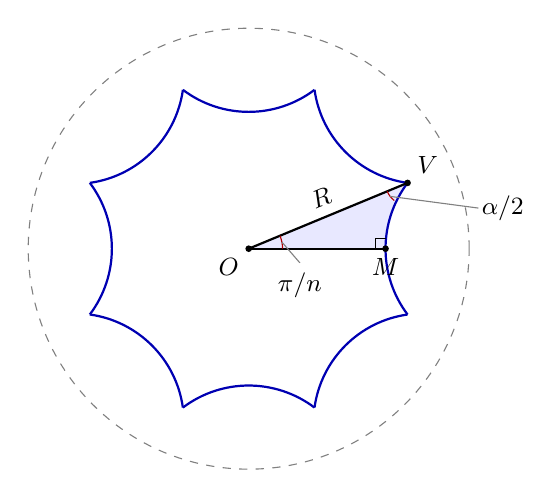
\begin{tikzpicture}[font=\small]
	\pgfmathsetmacro{\PlotRadius}{2.8}
	\pgfmathsetmacro{\VertexRadius}{.78}
	\pgfmathsetmacro{\HalfAngle}{22.5}
	\pgfmathsetmacro{\CircleCenter}{(1+\VertexRadius^2)/(2*\VertexRadius*cos(\HalfAngle))}
	\pgfmathsetmacro{\CircleRadius}{sqrt(\CircleCenter^2-1)}
	\pgfmathsetmacro{\ArcAngle}{atan2(\VertexRadius*sin(\HalfAngle),\CircleCenter-\VertexRadius*cos(\HalfAngle))}
	\pgfmathsetmacro{\Midpoint}{\PlotRadius*(\CircleCenter-\CircleRadius)}
	\coordinate (O) at (0,0);
	\coordinate (M) at (\Midpoint,0);
	\coordinate (V) at ({\PlotRadius*\VertexRadius*cos(\HalfAngle)},{\PlotRadius*\VertexRadius*sin(\HalfAngle)});
	\fill[blue!9] (O)--(M) arc[start angle=180,end angle={180-\ArcAngle},radius={\PlotRadius*\CircleRadius}]--cycle;
	\draw[dashed,gray] (O) circle (\PlotRadius);
	\foreach \j in {0,...,7}{
		\pgfmathsetmacro{\MiddleAngle}{45*\j}
		\draw[thick,blue!70!black] ({\PlotRadius*\VertexRadius*cos(\MiddleAngle-\HalfAngle)},{\PlotRadius*\VertexRadius*sin(\MiddleAngle-\HalfAngle)}) arc[start angle={\MiddleAngle+180+\ArcAngle},end angle={\MiddleAngle+180-\ArcAngle},radius={\PlotRadius*\CircleRadius}];
	}
	\draw[thick] (O)--(M);
	\draw[thick] (O)--node[midway,above,sloped] {\(R\)}(V);
	\draw (\Midpoint-.13,0)--(\Midpoint-.13,.13)--(\Midpoint,.13);
	\draw[red!70!black] (.43,0) arc[start angle=0,end angle=\HalfAngle,radius=.43];
	\node[below] at (.65,-.18) {\(\pi/n\)};
	\draw[thin,gray] (.65,-.18)--({.43*cos(\HalfAngle/2)},{.43*sin(\HalfAngle/2)});
	\begin{scope}[shift={(V)}]
		\draw[red!70!black] ({.28*cos(180+\HalfAngle)},{.28*sin(180+\HalfAngle)}) arc[start angle={180+\HalfAngle},end angle={270-\ArcAngle},radius=.28];
		\draw[thin,gray] ({.28*cos((450+\HalfAngle-\ArcAngle)/2)},{.28*sin((450+\HalfAngle-\ArcAngle)/2)})--(.9,-.32);
		\node[right,fill=white,inner sep=1pt] at (.9,-.32) {\(\alpha/2\)};
	\end{scope}
	\foreach \p in {O,M,V}{\fill (\p) circle (1.2pt);}
	\node[below left] at (O) {\(O\)};
	\node[below] at (M) {\(M\)};
	\node[above right] at (V) {\(V\)};
\end{tikzpicture}

	\caption[正则双曲多边形的直角三角形]{圆盘模型中的正则八边形。中心 \(O\)、边中点 \(M\) 与顶点 \(V\) 构成直角三角形，\(OV=R\)，中心角为 \(\pi/n\)，顶点角为 \(\alpha/2\)。虚线圆周是理想边界；测地边向圆盘中心一侧弯曲。}
	\label{g1:fig:regular-hyperbolic-polygon}
\end{figure}

角条件在粘合时有直接含义。若若干多边形顶点被识别成一个点，它们围出的角必须合计 \(2\pi\)，才可能成为普通光滑曲面点；否则会留下圆锥型的角亏或角盈。上面的 \(4g\) 个角之和正是 \(2\pi\)，而边长相等允许按保向等距匹配有序端点。下一节还会逐项检查边两侧的光滑接合、顶点邻域以及整体商空间；这里的多边形构造提供了所需的具体长度与角度数据。

% !TeX root = ../../Book1.tex
% 纲要标题：### 10.2 离散群与曲面商
% 纲要位置：几何学计划纲要.md，第 515 行。
% 正文状态：初稿；尚未正式审核。

% 纲要内容开始
% 
% * 椭圆、抛物和双曲变换
% * 自由固有作用及基本区域
% * 基本多边形的边配对与粘合
% * 闭曲面、尖点与漏斗的模型
% 
% 纲要内容结束

\section{离散群与曲面商}
\label{g1:sec:1002}

双曲平面中每一点的局部几何都相同，但把不同的点按等距变换识别以后，可以得到有闭测地线的圆柱、面积有限的尖点端，乃至任意亏格不小于二的闭曲面。这里有两个不同的构造问题：给定一个等距变换群，商是否仍是光滑曲面；给定一张多边形和边配对，接缝及顶点附近的度量是否光滑。前一个问题由作用的自由性和固有性控制，后一个问题必须逐条检查边的等距配对和顶点周围的总角。

\subsection{椭圆、抛物和双曲变换}
\label{g1:subsec:1002:01}

在上半平面 \(\mathbb H=\{z=x+iy:y>0\}\) 上，度量为 \(g_{\mathbb H}=|\mathrm{d}z|^2/y^2\)。\cref{g1:thm:hyperbolic-isometry-group}已经说明，其保向等距变换恰为
\[
	z\longmapsto\frac{az+b}{cz+d},\qquad
	A=\begin{pmatrix}a&b\\c&d\end{pmatrix}\in\operatorname{SL}(2,\mathbb R),
\]
其中 \(A\) 与 \(-A\) 给出同一个变换，因此群为 \(\operatorname{PSL}(2,\mathbb R)\)。这些变换也作用于理想边界 \(\mathbb R\cup\{\infty\}\)；那里不是双曲平面的一部分，边界不动点与平面内不动点必须区别。

\begin{theorem}[保向等距变换的分类]\label{g1:thm:psl-element-classification}
	设 \(h\in\operatorname{PSL}(2,\mathbb R)\) 不是恒等变换，取代表矩阵 \(A\in\operatorname{SL}(2,\mathbb R)\)，记 \(\tau=(\operatorname{tr}A)^2\)。则有且仅有下列一种情形。
	\begin{enumerate}
		\item \(\tau<4\)：\(h\) 在 \(\mathbb H\) 中有唯一不动点，在理想边界没有不动点；移到圆盘模型并把该点移到原点后，\(h\) 为非恒等旋转 \(w\mapsto e^{i\theta}w\)。称 \(h\) 为\term[tuoyuanbianhuan]{椭圆变换}[elliptic isometry]。
		\item \(\tau=4\)：\(h\) 在 \(\mathbb H\) 中没有不动点，在理想边界有唯一不动点；经保向等距共轭后，\(h\) 为 \(z\mapsto z+1\) 或 \(z\mapsto z-1\)。称 \(h\) 为\term[paowubianhuan]{抛物变换}[parabolic isometry]。
		\item \(\tau>4\)：\(h\) 在 \(\mathbb H\) 中没有不动点，在理想边界有两个不同不动点；经保向等距共轭后，\(h\) 为 \(z\mapsto e^\ell z\)，其中 \(\ell>0\) 且
		\[
			|\operatorname{tr}A|=2\cosh(\ell/2).
		\]
		称 \(h\) 为\term[shuangqubianhuan]{双曲变换}[hyperbolic isometry]。
	\end{enumerate}
\end{theorem}
\begin{proof}
	更换代表 \(A\mapsto-A\) 不改变 \(\tau\)，共轭也不改变它。有限不动点满足
	\[
		cz^2+(d-a)z-b=0,
	\]
	其判别式为 \((a+d)^2-4(ad-bc)=\tau-4\)。若 \(c=0\)，还要把无穷远点计入；统一地说，理想边界不动点就是实矩阵 \(A\) 的实特征直线，所以判别式同样区分零个、一个和两个实不动点。

	若 \(\tau<4\)，两个非实根互为共轭，恰有一个在 \(\mathbb H\) 中。设它为 \(p=x+iy\)，变换 \(z\mapsto(z-x)/y\) 将其送到 \(i\)。一个实 Möbius 变换固定 \(i\) 当且仅当其代表可写成
	\[
		R_\theta=\begin{pmatrix}
			\cos(\theta/2)&\sin(\theta/2)\\
			-\sin(\theta/2)&\cos(\theta/2)
		\end{pmatrix}.
	\]
	用圆盘坐标 \(w=(z-i)/(z+i)\) 代入，所得变换为 \(w\mapsto e^{i\theta}w\)。非恒等性排除 \(\theta\equiv0\pmod{2\pi}\)，也给出平面内不动点的唯一性。

	若 \(\tau=4\)，非恒等性说明 \(A\ne\pm I\)，故只有一条实特征直线。将它送到 \(\infty\)，变换便写成 \(z\mapsto a^2z+ab\)，其中代表矩阵的对角元为 \(a,a^{-1}\)。迹平方等于四迫使 \(a=\pm1\)，于是它是非零平移 \(z\mapsto z+t\)。再用正缩放共轭，将 \(|t|\) 变成 \(1\)。正、负两个方向都保留在陈述中，因为保向共轭不能随意把这两个标准型混为同一个。

	若 \(\tau>4\)，将两个理想不动点送到 \(0,\infty\)，得到 \(z\mapsto\lambda z\)，其中 \(\lambda>0\) 且 \(\lambda\ne1\)。若 \(\lambda<1\)，再用 \(z\mapsto-1/z\) 交换两端，便可令 \(\lambda=e^\ell>1\)。代表矩阵可取 \(\operatorname{diag}(e^{\ell/2},e^{-\ell/2})\)，给出迹的公式。三个标准型的全部不动点均已列出，证明分类。
\end{proof}

迹平方判别的是三种类型，不是所有共轭参数。例如圆盘中旋转 \(\theta\) 与旋转 \(-\theta\) 具有相同的迹平方，但保向共轭还保留旋转方向。下一步要构造商时，更重要的是一个变换把点移动了多远。

\begin{definition}[平移长度]\label{g1:def:hyperbolic-translation-length}
	设 \(\mathbb H\) 为曲率 \(-1\) 的双曲平面，\(d_{\mathbb H}\) 为其长度距离，\(h:\mathbb H\to\mathbb H\) 为等距变换。它的\term[pingyichangdu]{平移长度}[translation length]定义为
	\[
		L(h)=\inf_{p\in\mathbb H}d_{\mathbb H}(p,hp).
	\]
\end{definition}

对椭圆变换，\(L(h)=0\)，且在唯一内点不动点处达到。对抛物变换 \(z\mapsto z+t\)，\cref{g1:thm:hyperbolic-distance-geodesics}中的距离公式给出
\[
	\cosh d_{\mathbb H}(z,z+t)=1+\frac{t^2}{2y^2},
\]
所以 \(L(h)=0\)，但没有任何平面内点达到这个下确界。对双曲标准型，距离公式则给出
\begin{equation}\label{g1:eq:hyperbolic-displacement}
	\cosh d_{\mathbb H}(z,e^\ell z)
	=\cosh\ell+2\sinh^2(\ell/2)\frac{x^2}{y^2}.
\end{equation}
因此 \(L(h)=\ell\)，恰在虚轴上达到。一般双曲变换的两个理想不动点之间的测地线称为它的\term[zhou]{轴}[axis]；沿轴的作用就是长度为 \(\ell\) 的平移。下确界是否达到，已经把抛物与双曲两种无内点不动点的行为区别开来。

\subsection{自由固有作用及基本区域}
\label{g1:subsec:1002:02}

为了使商附近仍是一张普通小圆盘，需要排除两种障碍：一个群元素固定该点，或者无限多个不同群元素在附近反复堆积。前者由自由性排除，后者由下面的紧集条件控制。

\begin{definition}[离散子群与固有作用]\label{g1:def:discrete-proper-isometric-action}
	给 \(\operatorname{PSL}(2,\mathbb R)\) 赋予矩阵群模去 \(\{\pm I\}\) 的拓扑。若子群 \(\Gamma\) 有一个单位元邻域只包含其单位元，就称它为\term[lisanziqun]{离散子群}[discrete subgroup]。对群在 \(\mathbb H\) 上的作用，若 \(\gamma p=p\) 蕴含 \(\gamma=1\)，就称它为\term[ziyouzuoyong]{自由作用}[free action]；若对每个紧集 \(K\subset\mathbb H\)，集合
	\[
		\{\gamma\in\Gamma:\gamma K\cap K\ne\varnothing\}
	\]
	有限，就称它为\term[guyouzuoyong]{固有作用}[proper action]。
\end{definition}

这里把 \(\Gamma\) 当作离散群，使用的是适合离散作用的紧集定义。第五章\cref{g1:def:properly-discontinuous-covering}中的“适当不连续”还要求每点都有与所有非平凡平移不交的小邻域，因而已经包含自由性。本节的固有性允许有限稳定子；要恢复第五章的条件，需要同时假设自由。

\begin{proposition}[离散性与固有性]\label{g1:prop:discrete-hyperbolic-action}
	子群 \(\Gamma\subset\operatorname{PSL}(2,\mathbb R)\) 离散，当且仅当其在 \(\mathbb H\) 上的作用固有。离散子群中的椭圆元素都有有限阶；其作用自由，当且仅当它没有非单位有限阶元素。
\end{proposition}
\begin{proof}
	先说明离散子群与任意紧的群元素集合只有有限交。若紧集内有无限个不同元素 \(\gamma_n\)，由矩阵空间的紧性可取收敛子列；于是不同的 \(\gamma_n^{-1}\gamma_m\) 可以任意接近单位元，与单位元孤立矛盾。这里并未假定子群先验闭；同一个论证也说明其在矩阵群中的任何收敛序列最终恒定，所以它确实闭。

	给 \(p=x+iy\) 选连续依赖于 \(p\) 的等距变换
	\[
		u_p(z)=yz+x,\qquad
		u_p=\left[\begin{pmatrix}\sqrt y&x/\sqrt y\\0&1/\sqrt y\end{pmatrix}\right],
	\]
	它将 \(i\) 送到 \(p\)。若 \(h p=q\)，则 \(u_q^{-1}hu_p\) 固定 \(i\)，故属于前面写出的旋转群 \(\{R_\theta\}\)，这是一个紧群。若 \(p,q\in K\)，那么 \(h\) 位于紧集
	\[
		\{u_qR_\theta u_p^{-1}:p,q\in K,\ 0\le\theta\le2\pi\}
	\]
	之中。离散子群与该紧集只有有限交，故作用固有。反过来，若有不同的 \(\gamma_n\) 趋于单位元，则 \(\gamma_ni\to i\)；包含这些点和 \(i\) 的一个小紧邻域 \(K\) 将满足 \(\gamma_nK\cap K\ne\varnothing\)，与固有性矛盾。

	椭圆元素的所有幂都位于一个共轭旋转群中，后者紧，所以离散性迫使其幂只有有限多个，即该元素为有限阶。分类定理表明，非恒等抛物或双曲变换都有无限阶。因此没有非单位有限阶元素等价于没有椭圆元素，又等价于没有平面内不动点，即作用自由。
\end{proof}

例如绕同一点旋转 \(2\pi/m\) 生成的有限群离散且作用固有，却不自由；这个点在商中有锥角 \(2\pi/m\)。绕同一点旋转一个与 \(2\pi\) 之比为无理数的角所生成的群则不离散，因为它有无限多个幂落在同一个紧旋转群中。离散性不会自动排除所有不动点。

\begin{theorem}[自由固有等距作用的商]\label{g1:thm:hyperbolic-quotient}
	设 \(\Gamma\subset\operatorname{PSL}(2,\mathbb R)\) 自由且固有地作用于 \(\mathbb H\)。则轨道商 \(M=\mathbb H/\Gamma\) 是 Hausdorff、第二可数的可定向光滑曲面，且有唯一度量使投影 \(q:\mathbb H\to M\) 为局部等距。该度量曲率恒为 \(-1\)，长度距离完备；\(q\) 是万有覆盖，覆盖变换群恰为 \(\Gamma\)。
\end{theorem}
\begin{proof}
	固定 \(p\in\mathbb H\)，取包含它的紧邻域 \(K\)。只有有限个 \(\gamma\) 满足 \(\gamma K\cap K\ne\varnothing\)。自由性给出 \(\gamma p\ne p\)；对有限个这样的非单位元素，同时缩小 \(p\) 的邻域 \(U\)，即可使 \(\gamma U\cap U=\varnothing\)。其余元素由 \(U\subset K\) 已经排除。因此第五章的强适当不连续条件成立。\cref{g1:prop:action-quotient-cover}的证明给出 \(q\) 为开映射，以及
	\[
		q^{-1}(q(U))=\bigsqcup_{\gamma\in\Gamma}\gamma U,
	\]
	每张片都同胚映到 \(q(U)\)。上半平面凸且可缩，特别是单连通；该命题还说明这是万有覆盖，覆盖变换群正是 \(\Gamma\)。

	仍须核验商的分离性。若 \(p,r\) 不在同一轨道，取它们的紧邻域之并 \(K\)。可能把第一个邻域送到第二个的群元素只有有限个；又因 \(\gamma p\ne r\)，可以同时缩小成 \(U\ni p,V\ni r\)，使所有 \(\gamma U\) 都不交 \(V\)。于是 \(q(U),q(V)\) 是不交开邻域，故商 Hausdorff。\(\mathbb H\) 的可数开基经开映射 \(q\) 取像，仍是商的可数开基，得到第二可数性。

	用 \(q|_U\) 的逆把 \(q(U)\) 当作上半平面小片。两个这样的图在每个足够小的交叠部分上相差唯一一个 \(\gamma\in\Gamma\)，因而转换是光滑保向等距。各片的度量便相容地下降，唯一性也由局部等距要求决定；局部曲率保持为 \(-1\)。

	最后证明完备性，而不由“局部等距”直接推出。距离公式说明 \(d_{\mathbb H}(i,x+iy)\le R\) 等价于
	\[
		x^2+(y-\cosh R)^2\le\sinh^2R.
	\]
	这个 Euclid 闭圆盘的最低高度为 \(e^{-R}>0\)，所以双曲闭球紧。固有性于是保证轨道与每个闭有界球只有有限交，故
	\begin{equation}\label{g1:eq:hyperbolic-quotient-distance}
		d_M(qx,qy)=\min_{\gamma\in\Gamma}d_{\mathbb H}(x,\gamma y).
	\end{equation}
	具体地，右端的最小值存在；不同轨道之间它为正，三角不等式由等距不变性得到。投影任意连接 \(x\) 与 \(\gamma y\) 的测地段，说明商长度距离不超过它。反过来，商中的每条分片光滑连接曲线从 \(x\) 提升后终于某个 \(\gamma y\)，提升保持长度，故其长度至少为右端。这样就证明了等式。

	对 \(M\) 中任一 Cauchy 序列，取子列 \(p_n\)，使 \(d_M(p_n,p_{n+1})<2^{-n}\)。从任意提升 \(x_1\) 开始，逐次用\eqref{g1:eq:hyperbolic-quotient-distance}选择提升 \(x_{n+1}\)，满足 \(d_{\mathbb H}(x_n,x_{n+1})<2^{-n}\)。这些提升构成 Cauchy 序列，在完备的 \(\mathbb H\) 中收敛；其投影给出 \(p_n\) 的极限。原序列因 Cauchy 性也收敛，故商完备。
\end{proof}

上述证明把拓扑和度量的责任分开了：局部不交邻域给出覆盖，固有性还保证不同轨道能被分离，而等距性才使局部度量在商上相容。

\begin{definition}[Dirichlet 区域]\label{g1:def:dirichlet-domain}
	设 \(\Gamma\subset\operatorname{PSL}(2,\mathbb R)\) 的作用自由且固有，固定 \(p\in\mathbb H\)。集合
	\[
		D_p=\{x\in\mathbb H:d_{\mathbb H}(x,p)\le d_{\mathbb H}(x,\gamma p)\ \text{对所有 }\gamma\in\Gamma\}
	\]
	称为以 \(p\) 为中心的\term[Dirichletquyu]{Dirichlet 区域}[Dirichlet domain]。它把“离哪一个轨道点最近”转化成一组半平面条件。\footnote{Johann Peter Gustav Lejeune Dirichlet（1805--1859），德国数学家，对数论、Fourier 级数与势理论作出重要贡献。}
\end{definition}

\begin{proposition}[Dirichlet 区域的铺盖]\label{g1:prop:dirichlet-domain}
	设 \(\Gamma\subseteq\operatorname{PSL}(2,\mathbb R)\) 以标准双曲等距自由且固有地作用于 \(\mathbb H\)，\(p\in\mathbb H\)，\(d\) 为双曲距离。令 \(D_p=\{x\in\mathbb H:d(x,p)\le d(x,\gamma p)\text{ 对所有 }\gamma\in\Gamma\}\)。则 \(D_p\) 是有非空内部的闭测地凸集，所有 \(\gamma D_p\) 覆盖 \(\mathbb H\)，不同平移的内部不交；这些平移局部有限。\(D_p\) 在每个有界部分由有限条测地边界限制。若 \(\mathbb H/\Gamma\) 紧，则 \(D_p\) 是紧的有限边测地多边形。
\end{proposition}
\begin{proof}
	两个不同点 \(p,q\) 的等距轨迹是一条测地线，\(d(x,p)\le d(x,q)\) 选出包含 \(p\) 的闭半平面。在双曲面模型中可以直接看出这一点：距离公式把等距条件写成 Lorentz 内积的线性等式 \(\langle X,P-Q\rangle_L=0\)，而 \(P-Q\) 为空间样向量；该平面截双曲面得到测地线。每一侧测地凸，因为长为 \(L>0\) 的测地段在双曲面上的表达是
	\[
		X(t)=\frac{\sinh((1-t)L)}{\sinh L}X(0)
		+\frac{\sinh(tL)}{\sinh L}X(1),\qquad 0\le t\le1,
	\]
	两系数均非负，保持同侧的线性不等式。因此 \(D_p\) 是闭测地凸集。固有性和自由性给出 \(\inf_{\gamma\ne1}d(p,\gamma p)>0\)，取该下界一半以内的小球，就包含在 \(D_p\) 的内部。

	对任意 \(x\)，轨道 \(\Gamma p\) 中有一个距 \(x\) 最近的点，存在性与商距离的最小值相同。若最近点为 \(\gamma p\)，则 \(\gamma^{-1}x\in D_p\)，所以各平移覆盖。若 \(x\) 同时位于 \(\gamma D_p\) 和 \(\eta D_p\) 的内部，且 \(\gamma\ne\eta\)，第一个内部条件给出 \(d(x,\gamma p)<d(x,\eta p)\)，第二个给出反向严格不等式，矛盾。严格性来自等距轨迹是一条边界测地线，不能包含内点。

	若 \(x\in\overline B(p,R)\cap\gamma D_p\)，最近点条件说明 \(d(x,\gamma p)\le d(x,p)\le R\)，于是 \(d(p,\gamma p)\le2R\)。这样的 \(\gamma\) 只有有限个，得到平移的局部有限性。同样，在 \(B(p,R)\) 内能限制 \(D_p\) 的半平面只可能来自 \(d(p,\gamma p)\le2R\) 的元素，因为更远的轨道点在此球中总比 \(p\) 远。因此每个有界部分只需有限条边界。

	若商紧，递增开集 \(q(B(p,R))\) 覆盖它，紧性给出某个 \(R\) 已经覆盖全商。每个 \(x\in D_p\) 都与 \(B(p,R)\) 中某点等价，故它距某个轨道点小于 \(R\)，最近点条件进一步给出 \(d(x,p)<R\)。于是 \(D_p\) 闭且有界，从而紧；它全部位于一个稍大的球内，所需边界只有有限条，得到有限测地多边形。
\end{proof}

满足覆盖且内部不重叠的这样的闭区域称为群作用的\term[jibenquyu]{基本区域}[fundamental domain]。边界上可以有多个代表，必须按群元素识别，不能要求每条轨道与闭区域恰交一次。非紧商的 Dirichlet 区域也未必只有有限条边，上命题只保证有界范围内的有限性。

\subsection{基本多边形的边配对与粘合}
\label{g1:subsec:1002:03}

反过来，可以先画一张双曲多边形，再沿成对的边接合。第六章\cref{g1:thm:surface-polygon}及\cref{g1:prop:orientable-standard-word}解释了边字如何记录拓扑粘合；现在还要使这些粘合保留度量。边内点的邻域由两张半圆盘组成，顶点的邻域则由若干个角扇组成，两处需要不同的检查。

\begin{proposition}[双曲多边形的光滑粘合]\label{g1:prop:hyperbolic-polygon-gluing}
	设 \(P\subset\mathbb H\) 是紧凸测地多边形，将不同的边两两配对，每对等长，并用保向双曲等距变换按相反的边界行进方向识别。对每个顶点等价类，将其各角的一条小圆弧按边配对接起；假设所得空间是一条圆周，且该类内的角度总和为 \(2\pi\)。则商 \(P/{\sim}\) 是紧、可定向、无边界的光滑曲面，\(P\) 的双曲度量在其上光滑粘合，曲率恒为 \(-1\)。
\end{proposition}
\begin{proof}
	等长测地边的端点可以按要求配对：先用\cref{g1:prop:model-isometry-data}将一条边的起点及单位切向量送到另一条边的终点及反向单位切向量；测地线的初值唯一性使整条等长边随之对应。保向性保证原来的内侧被送到另一条边的外侧，因此两侧窄半盘在识别后确实拼成一个双曲小圆盘，度量在接缝处光滑。

	这里的商也是 Hausdorff。等价关系在 \(P\times P\) 中由对角线、有限个闭边配对映射的图以及有限个顶点等价对组成，故为闭集。若 \(C\subset P\) 闭，它的饱和集是此闭关系与 \(C\times P\) 的交在第二因子的投影，因紧性而闭。两个不同等价类是 \(P\) 中不交的有限集，取不交开邻域 \(U,V\) 包含它们；从 \(U\) 中去掉所有与 \(P\setminus U\) 等价的点，得到包含原等价类的饱和开集，\(V\) 同理。两者下降为商中不交开邻域。商紧性来自 \(P\) 的紧性。

	在一个顶点类处，将各原顶点附近截成同样小半径的角扇。边等距保留距相应顶点的距离，故各扇可以用同一个径向变量 \(r\) 粘合。双曲面极坐标
	\[
		(r,\theta)\longmapsto(\cosh r,\sinh r\cos\theta,\sinh r\sin\theta)
	\]
	直接给出度量 \(\mathrm{d}r^2+\sinh^2r\,\mathrm{d}\theta^2\)。把各扇按圆弧连接的次序排好，角变量逐段累计；小圆弧接成一条圆周意味着绕行只形成一个扇环，总角 \(2\pi\) 则使这个扇环恰好拼成普通双曲小圆盘。末缝处 \(\theta=0\) 与 \(2\pi\) 的极坐标映射以及所有导数相容，中心也由上述双曲面坐标给出通常的光滑结构。因此顶点没有锥形奇点。

	面内、边内和顶点处的这些局部图在交叠处相差双曲等距变换，形成相容的光滑图册和度量。各边都已配对，故没有边界；配对反转边界行进方向而保持环境定向，所以局部定向也相容。紧性允许从局部图取有限覆盖，每张图有可数基，故商第二可数。这就得到所述光滑度量曲面。
\end{proof}

顶点附近的小圆弧拼成的圆周常称为该顶点的\term[lianjie]{链接}[link]。链接控制局部邻域是不是一张盘，总角则控制这张盘上的度量是否光滑。若链接仍是一条圆周但总角为 \(\Theta\ne2\pi\)，小半径圆周的长度就是 \(\Theta\sinh r\)，除以半径后趋于 \(\Theta\)，不能是光滑曲面中应有的 \(2\pi\)。因此检查边长相等还不够。

\ProseParagraphBreak

这一命题构造的是有限多边形的度量商。若另把边配对变换放进 \(\operatorname{PSL}(2,\mathbb R)\) 并取它们生成的群，还需要证明其离散性及原多边形的平移是否铺盖整个平面；这些整体结论不是一句“角和为 \(2\pi\)”就能直接替代的。下一节将用展开映射说明完备模型结构的整体实现。

\begin{theorem}[闭双曲曲面的多边形构造]\label{g1:thm:closed-hyperbolic-polygon}
	设 \(g\ge2\) 为整数，\(\Sigma_{g,0}\) 为可定向亏格 \(g\) 的闭曲面。存在一张与 \(\Sigma_{g,0}\) 同胚的紧光滑曲面，带曲率恒为 \(-1\) 的度量。它可以由曲率 \(-1\) 双曲平面中一个内角均为 \(\pi/(2g)\) 的凸正则测地 \(4g\) 边形按边字
	\[
		a_1b_1a_1^{-1}b_1^{-1}\cdots a_gb_ga_g^{-1}b_g^{-1}
	\]
	将同字母边按相反边界方向，用保向双曲等距两两配对得到，面积为 \(4\pi(g-1)\)。
\end{theorem}
\begin{proof}
	\cref{g1:prop:regular-hyperbolic-polygons}保证：给定 \(n\ge3\) 及 \(0<\alpha<(n-2)\pi/n\)，存在内角为 \(\alpha\) 的正则双曲 \(n\) 边形。对 \(n=4g\)、\(\alpha=\pi/(2g)\)，所需严格不等式恰由 \(g\ge2\) 保证。所有边等长，故按上命题可实施指定的等距配对。

	还要检查顶点，不能只因共有 \(4g\) 个角就默认它们拼在同一点。依次记顶点为 \(v_0,\ldots,v_{4g-1}\)，第 \(j\) 条边从 \(v_j\) 指向 \(v_{j+1}\)，下标模 \(4g\)。在第 \(k\) 个四边块中，\(a\) 配对给出
	\[
		v_{4k}\sim v_{4k+3},\qquad v_{4k+1}\sim v_{4k+2},
	\]
	\(b\) 配对给出 \(v_{4k+1}\sim v_{4k+4}\) 及 \(v_{4k+2}\sim v_{4k+3}\)。这些关系把该块的五个连续端点连在一起，因而所有顶点属于一个等价类。

	再从一个角的小圆弧穿过配对边进入下一个角，所得链接的后继顺序为
	\[
		4k+1\longmapsto4k+2\longmapsto4k+3\longmapsto4k
		\longmapsto4(k-1)+1
	\]
	（所有下标模 \(4g\)）。它先走过一个四边块的四个角，再进入前一个四边块，最终恰走过全部 \(4g\) 个角一次才返回，故链接是单一圆周。总角为 \(4g\cdot\pi/(2g)=2\pi\)，上命题给出光滑双曲度量。

	这个边字的拓扑类型由\cref{g1:prop:orientable-standard-word}中标准字与手柄连通和的对应给出，正是 \(\Sigma_{g,0}\)。最后，\cref{g1:prop:geodesic-polygon-area}给出
	\[
		\operatorname{Area}(P)=(4g-2)\pi-4g\frac{\pi}{2g}=4\pi(g-1).
	\]
	边及顶点的识别不改变面积，故商也有这个面积。
\end{proof}

对 \(g=1\)，所需四边形的四个角都为 \(\pi/2\)，角和达到平面四边形的角和 \(2\pi\)，双曲面积公式将给出零面积，所以这种非退化双曲四边形不存在。这与第九章 Gauss--Bonnet 排除闭环面上的负常曲率度量相符。

\subsection{闭曲面、尖点与漏斗的模型}
\label{g1:subsec:1002:04}

刚才得到的闭曲面紧，长度距离因而完备：局部双曲图中的度量在小闭片上与 Euclid 度量双边可比，长度距离给出原拓扑；任一 Cauchy 序列都有由紧性提供的收敛子列，进而整个序列收敛。它们的面积有限，但非紧曲面也可能有有限面积的端部。两种最简单的非紧端部来自抛物和双曲循环群。

\begin{example}[尖点]\label{g1:exm:hyperbolic-cusp}
	令 \(T(z)=z+1\)。群 \(\langle T\rangle\) 离散且自由，整个商 \(\mathbb H/\langle T\rangle\) 是完备双曲圆柱。固定 \(Y>0\)，取其中由 \(y\ge Y\) 给出的端部
	\[
		C_Y=\{y\ge Y\}/\langle T\rangle.
	\]
	这是\term[jiandian]{尖点}[cusp]的标准模型。其一条基本条带为 \(0\le x\le1,y\ge Y\)，两条竖边配对。令 \(r=\log(y/Y)\)，则
	\begin{equation}\label{g1:eq:hyperbolic-cusp-metric}
		g=\mathrm{d}r^2+Y^{-2}e^{-2r}\,\mathrm{d}x^2,
		\qquad r\ge0,\quad x\in\mathbb R/\mathbb Z.
	\end{equation}
	截圈 \(r=R\) 的长度为 \(Y^{-1}e^{-R}\)，向尖端越来越短；但是任何向 \(r\to\infty\) 行进的曲线长度至少为其 \(r\) 的总变化，所以尖端处在无限距离处。另一方面，
	\[
		\operatorname{Area}(C_Y)=\int_0^1\int_Y^\infty\frac{\mathrm{d}y\,\mathrm{d}x}{y^2}=\frac1Y.
	\]
	因此无限距离与有限面积可以同时出现。这里 \(C_Y\) 是带截口的端部；整个完备平移商还包含 \(0<y<Y\) 的另一端，其面积无限。不能把有限面积端部和整个圆柱的面积混为一谈。
\end{example}

\begin{proposition}[双曲圆柱的 Fermi 坐标]\label{g1:prop:hyperbolic-cylinder-fermi}
	设 \(\ell>0\)，令 \(H(z)=e^\ell z\)。完备双曲圆柱 \(\mathbb H/\langle H\rangle\) 有全局坐标
	\[
		r\in\mathbb R,\qquad t\in\mathbb R/\ell\mathbb Z,
		\qquad g=\mathrm{d}r^2+\cosh^2r\,\mathrm{d}t^2.
	\]
	\(r=0\) 是长度 \(\ell\) 的闭测地线，\(|r|\) 是距它的距离；\(r\ge0\) 与 \(r\le0\) 分别给出一个\term[loudou]{漏斗}[funnel]，各漏斗的面积无限。
\end{proposition}
\begin{proof}
	在 \(\mathbb H\) 中直接置
	\[
		x=e^t\tanh r,\qquad y=e^t\operatorname{sech}r.
	\]
	其逆为 \(t=\log\sqrt{x^2+y^2}\)、\(r=\operatorname{arsinh}(x/y)\)，所以这是全局坐标。求微分后交叉项抵消，得到
	\[
		\mathrm{d}x^2+\mathrm{d}y^2
		=e^{2t}\bigl(\mathrm{d}t^2+\operatorname{sech}^2r\,\mathrm{d}r^2\bigr).
	\]
	除以 \(y^2=e^{2t}\operatorname{sech}^2r\) 即得所述度量。缩放 \(z\mapsto e^\ell z\) 恰对应 \(t\mapsto t+\ell\)，故坐标下降到圆柱。群的离散性与自由性由缩放标准型直接得到，完备性由\cref{g1:thm:hyperbolic-quotient}保证。

	\(r=0\) 是虚轴的像，因而为闭测地线，其长度就是 \(t\) 的周期 \(\ell\)。任一从 \(r\) 到零的曲线长度至少为 \(|r|\)，固定 \(t\) 的径向段达到它，因此 \(|r|\) 是到轴的距离。在 \(r\ge0\) 一侧，截圈长度为 \(\ell\cosh r\)，面积元为 \(\cosh r\,\mathrm{d}r\,\mathrm{d}t\)，所以
	\[
		\operatorname{Area}(0\le r\le R)=\ell\sinh R\longrightarrow\infty.
	\]
	另一侧由 \(r\mapsto-r\) 对称得到相同结论。
\end{proof}

上述以测地线为基线、以法向距离 \(r\) 为横坐标的坐标称为\term[Fermizuobiao]{Fermi 坐标}[Fermi coordinates]。\footnote{Enrico Fermi（1901--1954），意大利出生的美国物理学家，研究量子理论、统计力学与核物理。}尖点截圈的长度指数衰减，漏斗截圈的长度按 \(\cosh r\) 增长，这是两种端部面积行为不同的直接原因。\cref{g1:fig:cusp-funnel-domains}把两个循环群的基本区域画在同一个上半平面模型中。

% !TeX root = ../Book1.tex
\begin{figure}[htbp]
	\centering
	\begin{tikzpicture}[scale=0.95,font=\small]
		\begin{scope}[xshift=-3.1cm]
			\fill[GeometryBlueLight] (0,0.9) rectangle (1.7,3.1);
			\draw[->] (-0.7,0)--(2.5,0) node[right] {\(x\)};
			\draw[GeometryBlue,thick] (0,0.35)--(0,3.25);
			\draw[GeometryBlue,thick] (1.7,0.35)--(1.7,3.25);
			\draw[GeometryBlue,dashed] (-0.4,0.9)--(2.1,0.9);
			\node[left] at (-0.4,0.9) {\(y=Y\)};
			\draw[->,GeometryBlue] (0,1.5)--(1.7,1.5) node[midway,above] {\(z\mapsto z+1\)};
			\draw[->,GeometryBlue] (0.85,2.2)--(0.85,3.2);
			\node[above] at (0.85,3.2) {尖端 \(y\to\infty\)};
			\node[below] at (0,0) {\(0\)};
			\node[below] at (1.7,0) {\(1\)};
			\node[align=center] at (0.85,-0.85) {平移商的尖点端\\竖边配对，阴影部分面积有限};
		\end{scope}
		\begin{scope}[xshift=3.7cm]
			\fill[GeometryBlueLight] (2.1,0) arc (0:180:2.1)--(-1.05,0) arc (180:0:1.05)--cycle;
			\draw[->] (-2.5,0)--(2.5,0) node[right] {\(x\)};
			\draw[GeometryBlue,thick] (2.1,0) arc (0:180:2.1);
			\draw[GeometryBlue,thick] (1.05,0) arc (0:180:1.05);
			\draw[GeometryGray,dashed] (0,0)--(0,2.7);
			\draw[GeometryBlue,very thick] (0,1.05)--(0,2.1);
			\node[right] at (0.06,1.6) {轴};
			\draw[->,GeometryBlue] (140:1.05)--(140:2.1);
			\node[above,align=center] at (-1.15,2.4) {\(z\mapsto e^\ell z\)};
			\node at (-1.5,0.45) {\(r<0\)};
			\node at (1.5,0.45) {\(r>0\)};
			\node[align=center] at (0,-0.85) {缩放商的基本区域\\两条半圆配对，轴两侧为漏斗};
		\end{scope}
	\end{tikzpicture}
	\caption[尖点与漏斗的基本区域]{左图截取 \(0\le x\le1,y\ge Y\)，仅表示平移商中的尖点端；右图取 \(1\le|z|\le e^\ell\)，表示整个缩放圆柱的一个基本区域。右图以半径比 \(2\) 示意，粗轴段配对后成为闭测地线。图中的 Euclid 大小不表示双曲长度。}
	\label{g1:fig:cusp-funnel-domains}
\end{figure}


闭曲面、尖点端和漏斗都具有相同的局部曲率 \(-1\)，它们的紧性、面积和环路长度却不同。模型与粘合给出了这些具体度量；若只知道一张抽象曲面处处局部等距于双曲平面，还不能省略展开及单值的论证就把它写成一个全局商。下一节将把这一环节独立证明。

% !TeX root = ../../Book1.tex
% 纲要标题：### 10.3 局部齐性结构及其单值
% 纲要位置：几何学计划纲要.md，第 522 行。
% 正文状态：初稿；尚未正式审核。

% 纲要内容开始
% 
% * 几何图册与过渡群
% * 展开映射的构造
% * 单值表示及等变性
% * 完备性与模型商的关系
% 
% ---
% 
% 纲要内容结束

\section{局部齐性结构及其单值}
\label{g1:sec:1003}

把一张平纸卷成圆柱，每一小片仍可摊回平面，但沿圆柱绕一圈以后，展开的位置会相差一个平移。这个差别不来自小片的曲率，而来自不同小片怎样拼接。前一节从模型中的群作用构造曲面，本节反过来从曲面上的局部模型出发，追踪一张图沿道路延续时如何变化。所得展开映射与单值表示将说明：什么时候局部模型确实能够拼成整个模型的商，什么时候只能得到一个不完备的局部结构。

\subsection{几何图册与过渡群}
\label{g1:subsec:1003:01}

本节的曲面均为非空、连通、无边界的 Hausdorff、第二可数曲面，沿用\cref{g1:def:topological-surface}的分离与可数条件。无边界的要求有实际作用：模型取整个 \(S^2,\mathbb R^2,\mathbb H^2\) 的开集，半圆盘边缘不在这类图册中。曲面局部道路连通，连通性因而保证道路连通；坐标小圆盘又保证局部单连通，能够使用第五章的万有覆盖。

\ProseParagraphBreak

先取连通光滑模型曲面 \(X\)，以及通过光滑微分同胚作用在 \(X\) 上的群 \(G\)。若只有单位元在整个 \(X\) 上逐点不动，就称该作用有效。本节还要求一个更强的局部确定性质：
\begin{equation}
	\label{g1:eq:model-local-determination}
	g|_O=h|_O,\quad O\subset X\text{ 非空开}
	\quad\Longrightarrow\quad g=h.
\end{equation}
有效性本身不足以推出这一点。一般光滑微分同胚可以在一个开集上为恒等，在远处才发生变化；此时从局部换图无法唯一恢复群元素。对于连通模型的等距群，\cref{g1:prop:isometry-initial-data}说明等距由一点及该点的导数决定，故满足\eqref{g1:eq:model-local-determination}。通常还要求 \(G\) 在 \(X\) 上传递，表示模型各点没有区别；下述延续构造实际使用的是局部确定性质。

\begin{definition}
	\label{g1:def:geometry-atlas}
	设 \(X\) 为连通光滑曲面，\(G\le\operatorname{Diff}(X)\)，并满足局部确定性：若 \(g,h\in G\) 在 \(X\) 的某个非空开集上一致，则 \(g=h\)。设 \(M\) 为无边界拓扑曲面，\(\{U_i\}\) 为它的开覆盖。\(M\) 的一个\term[jihetuce]{几何图册}[geometric atlas]，或 \((G,X)\) 图册，是覆盖 \(M\) 的图
	\[
		\varphi_i:U_i\longrightarrow\varphi_i(U_i)\subset X,
	\]
	其中各 \(\varphi_i\) 为到开集的同胚，而且在任意交叠 \(U_i\cap U_j\) 的每个连通分支 \(C\) 上，存在 \(g_{ij,C}\in G\)，使
	\[
		\varphi_i|_C=g_{ij,C}\circ\varphi_j|_C.
	\]
	两个图册若其并仍满足此条件，就称为相容。一个相容图册类称为 \(M\) 的\term[jubuqixingjiegou]{局部齐性结构}[locally homogeneous structure]或 \((G,X)\) 结构。
\end{definition}

这些图自动给出光滑结构，因为换图映射是光滑微分同胚的限制。交叠处的群元素由\eqref{g1:eq:model-local-determination}唯一确定；在三图的共同小邻域中，
\[
	g_{ik}=g_{ij}g_{jk}.
\]
这里群乘法是函数复合：\((gh)(x)=g(h(x))\)。只在每个交叠分支上指定元素，是为了允许交叠不连通；没有理由要求几个分支使用同一个元素。

\ProseParagraphBreak

若 \(X\) 带度量 \(g_X\)、\(G\le\operatorname{Isom}(X)\)，各片上的 \(\varphi_i^*g_X\) 在交叠处一致，故定义了 \(M\) 上的光滑度量。这是一个具体的粘合验证：\(g_{ij}\) 保持 \(g_X\)，所以
\[
	\varphi_i^*g_X=\varphi_j^*(g_{ij}^*g_X)=\varphi_j^*g_X.
\]
由此得到的曲面每点附近都与模型等距。若过渡群包含非等距变换，例如平面的伸缩，图册仍有意义，却不能用这个公式粘合 Euclid 度量。

常曲率度量是否真的给出这种图册，也需要一个桥梁。这个问题只涉及小邻域，可以直接使用第九章已经建立的测地极坐标。

\begin{proposition}[常曲率的局部模型]
	\label{g1:prop:constant-curvature-local-model}
	设 \(M\) 是无边界光滑度量曲面，Gauss 曲率恒为 \(\kappa\in\{1,0,-1\}\)。则每点附近分别局部等距于单位球面、Euclid 平面或曲率为 \(-1\) 的双曲平面。这些局部等距给出 \((\operatorname{Isom}(X),X)\) 图册；若 \(M\) 已定向，可将过渡群限制为保向等距群。
\end{proposition}
\begin{proof}
	固定 \(p\in M\)。由\cref{g1:prop:normal-neighborhood,g1:lem:gauss-lemma}，中心之外的测地极坐标具有度量
	\[
		\mathrm{d}r^2+a(r,\theta)^2\,\mathrm{d}\theta^2,\qquad a>0.
	\]
	局部取与 \((\partial_r,\partial_\theta)\) 一致的定向。令 \(e_1=\partial_r\)、\(e_2=a^{-1}\partial_\theta\)。度量的 Christoffel 公式给出 \(\nabla_{\partial_r}e_1=0\)、\(\nabla_{\partial_\theta}e_1=a_r e_2\)，所以本书约定的联络形式为 \(\omega=a_r\,\mathrm{d}\theta\)。由\cref{g1:prop:connection-curvature-form}，
	\[
		a_{rr}\,\mathrm{d}r\wedge\mathrm{d}\theta
		=\mathrm{d}\omega=-K a\,\mathrm{d}r\wedge\mathrm{d}\theta,
		\qquad a_{rr}+\kappa a=0.
	\]

	中心处的初值不能只从极坐标公式形式地代入。取 \(\mathrm{T}_pM\) 中的单位向量 \(e(\theta)=(\cos\theta,\sin\theta)\)。第九章的构造实际给出
	\[
		a(r,\theta)=r\,b(r,\theta),\qquad
		b(r,\theta)=\left|\mathrm{d}(\exp_p)_{re(\theta)}(e'(\theta))\right|.
	\]
	指数映射在零附近光滑，且其零点微分为恒等；因而被取范数的向量在零附近不为零，\(b\) 对 \(r,\theta\) 光滑且 \(b(0,\theta)=1\)。所以 \(a\) 从 \(r\ge0\) 一侧光滑延到零，并满足 \(a(0,\theta)=0\)、\(a_r(0,\theta)=1\)。由\cref{g1:lem:smooth-ode-flow}所含的一阶系统唯一性，固定 \(\theta\) 后该标量方程的解只能是
	\[
		a(r,\theta)=S_\kappa(r),\qquad
		S_1(r)=\sin r,\quad S_0(r)=r,\quad S_{-1}(r)=\sinh r.
	\]
	这些函数直接满足方程与初值，且不依赖 \(\theta\)。

	对应模型的曲率同为 \(\kappa\)，对它作上述计算得到相同极坐标度量。选模型点 \(o\) 及线性等距 \(A:\mathrm{T}_pM\to \mathrm{T}_oX\)，则
	\[
		F=\exp_o\circ A\circ\exp_p^{-1}
	\]
	在充分小的正常邻域内光滑。极坐标计算说明它在去掉中心后局部等距；在中心处，两个指数映射的微分均为恒等，故 \(\mathrm{d}F_p=A\) 也等距。这证明局部模型存在，并且没有留下极坐标在中心处的光滑性缺口。

	最后验证过渡图属于整个模型的等距群。在一个连通交叠分支上，过渡映射 \(f\) 是模型开集之间的局部等距。由\cref{g1:prop:model-isometry-data}的初值实现结论，存在全局模型等距 \(h\)，使它在某点的像及导数与 \(f\) 相同。局部等距保持协变导数：把联络经它搬运，仍度量相容且无挠，由\cref{g1:prop:surface-connection-properties}的唯一性就是原联络；因而它保持短测地线。测地线初值唯一性使 \(f,h\) 在该点附近相等。具有相同值及导数的点组成相对闭集，又由同样的短测地线论证为开集；连通性使它等于整个交叠分支。所以过渡映射确是 \(h\) 的限制。若曲面定向，最初选择保向 \(A\)，便只需保向标架与保向 \(h\)。
\end{proof}
\subsection{展开映射的构造}
\label{g1:subsec:1003:02}

固定基点 \(p_0\in M\)，并在其附近选一张初始图 \(\varphi_0\)。两张局部映射若在指定点的某个邻域内相等，称它们在该点有相同的\term[yingsheya]{映射芽}[germ of a map]。这里保留的是附近整张小图，而不只是点的像；点的像相同一般无法确定换图的群元素。我们只延续形如 \(a\circ\varphi_i\)、\(a\in G\) 的局部映射。

\begin{lemma}[图的沿路延续]
	\label{g1:lem:chart-continuation}
	设 \(X\) 为连通光滑曲面，\(G\le\operatorname{Diff}(X)\)，且任意 \(g,h\in G\) 若在某个非空开集上一致就有 \(g=h\)。设无边界曲面 \(M\) 带 \((G,X)\) 结构，\(\alpha:[0,1]\to M\) 连续，并在 \(\alpha(0)\) 给定一个相容的图芽。只允许延续为局部形如 \(a\circ\varphi_i\)、\(a\in G\) 的图芽，其中 \(\varphi_i\) 为结构图册中的图。该图芽可沿 \(\alpha\) 延续，且每个时刻的芽唯一。终点芽只依赖于 \(\alpha\) 的定端点同伦类。
\end{lemma}
\begin{proof}
	先构造延续。用图域覆盖道路像，将其拉回到紧区间；\cref{g1:lem:lebesgue-number}给出有限分割，使每一小段都包含在一张图中。在第一段按给定图芽调整这张图。若前段使用 \(a_i\varphi_i\)，下一段的接点附近满足 \(\varphi_i=g_{ij}\varphi_j\)，就取
	\[
		a_j=a_i g_{ij}.
	\]
	于是 \(a_i\varphi_i=a_j\varphi_j\) 在接点附近相等，两段确实接续。每个段内使用同一局部公式，就得到了沿整条道路的芽。

	为什么不受分割及中途换图影响？取任意两套延续并作公共细分；在每个足够短的参数区间内，把两套公式都换写在同一张图 \(\varphi\) 下，即 \(a\varphi\) 与 \(b\varphi\)。若它们在一个时刻的芽相同，就在非空开集上相等，\eqref{g1:eq:model-local-determination}强制 \(a=b\)，所以在该小段内始终相同。把这一结论沿有限分割推进，全部芽相同。这也证明在道路中插入反向再返回的小段不会改变延续结果。

	再处理同伦，而不是直接把“同伦”当成延续唯一性的另一种说法。设 \(H:[0,1]^2\to M\) 是定端点同伦；用图域的原像覆盖参数方形，取足够细的有限矩形网格，使每个闭小矩形的像落在一张图中。在一张图内，给定起始芽 \(a\varphi\) 后，沿任何道路到同一点都给出这个同一公式的芽。因此，沿一个小矩形的下边再右边，或沿左边再上边，产生相同的终点芽。

	从方形下边的网格路径开始，每次把某个小矩形的两条边替换为另两条边，逐格扫过一行，再扫过全部行，即可把下边连同右侧边替换为左侧边连同上边。每次替换保留延续芽；内部边若先后反向经过，则按上一段消去。左右侧在 \(H\) 下均为常值道路，因为同伦固定端点，它们不改变芽。因此下边与上边的延续有相同终点芽。这里有限网格的用途正是把任意连续同伦转成有限次、可核验的换路操作。
\end{proof}

现在把可能有不同延续结果的道路分开保存。由\cref{g1:thm:path-class-universal-cover}，曲面的万有覆盖可写为
\[
	\widetilde M=\{[\alpha]:\alpha(0)=p_0\},\qquad
	p([\alpha])=\alpha(1),
\]
其中同伦固定两端。记 \(\varphi_\alpha\) 为 \(\varphi_0\) 沿 \(\alpha\) 延续所得的终点图芽，定义
\begin{equation}
	\label{g1:eq:developing-definition}
	\operatorname{dev}([\alpha])=\varphi_\alpha(\alpha(1)).
\end{equation}
前一引理说明它良定义。这一映射称为\term[zhankaiyingshe]{展开映射}[developing map]。\symidx{\(\operatorname{dev}\)：几何结构的展开映射}

\ProseParagraphBreak

它为何是局部微分同胚，也可直接从第五章的道路类拓扑看出。在 \(\alpha(1)\) 取足够小的坐标圆盘 \(U\)，使终点芽由 \(f=a\varphi_i\) 在 \(U\) 上表示。\cref{g1:lem:path-class-basis}给出覆盖片
\[
	B([\alpha],U)=\{[\alpha*\beta]:\beta\text{ 在 }U\text{ 内从 }\alpha(1)\text{ 出发}\}.
\]
在这一片上，继续沿 \(\beta\) 不改变公式 \(f\)，所以 \(\operatorname{dev}=f\circ p\)。覆盖空间的光滑图由 \(p\) 拉回，\(p\) 在这一片上为微分同胚，\(f\) 也是微分同胚，因而展开映射局部光滑可逆。若过渡群保持 \(g_X\)，同一公式还说明 \(\operatorname{dev}\) 对拉回度量是局部等距。这里的“局部”不可省去：即使源空间单连通，展开映射仍可能重叠，也可能只覆盖模型的一部分。

\subsection{单值表示及等变性}
\label{g1:subsec:1003:03}

设 \(\gamma\) 是以 \(p_0\) 为基点的环路。其终点仍为 \(p_0\)，但延续后的图芽可能变成另一张图。该芽与初始图相容，故存在唯一 \(a_\gamma\in G\)，使
\[
	\varphi_\gamma=a_\gamma\circ\varphi_0
\]
在基点附近成立。图芽的同伦不变性说明 \(a_\gamma\) 只依赖 \([\gamma]\)。

\begin{theorem}[展开与单值]
	\label{g1:thm:developing-map}
	设 \(X\) 为连通光滑曲面，\(G\le\operatorname{Diff}(X)\)，且任意 \(g,h\in G\) 在某个非空开集上一致就有 \(g=h\)，即满足\eqref{g1:eq:model-local-determination}。设 \(M\) 为连通无边界曲面，带 \((G,X)\) 结构。固定 \(p_0\in M\) 及其相容初始图芽 \(\varphi_0\)，将从 \(p_0\) 出发的道路按定端点同伦取类，得到万有覆盖 \(\widetilde M\)。以 \(\varphi_\alpha\) 记沿 \(\alpha\) 延续的终点图芽，定义 \(\operatorname{dev}([\alpha])=\varphi_\alpha(\alpha(1))\)。对基点环路 \(\gamma\)，以唯一的 \(a_\gamma\in G\) 满足 \(\varphi_\gamma=a_\gamma\circ\varphi_0\)。则 \(\operatorname{dev}:\widetilde M\to X\) 为局部微分同胚，并给出群同态
	\[
		\rho:\pi_1(M,p_0)\longrightarrow G,\qquad \rho([\gamma])=a_\gamma.
	\]
	对道路类万有覆盖上的左覆盖变换作用 \(L_g[\alpha]=[\gamma*\alpha]\)、\(g=[\gamma]\)，有
	\begin{equation}
		\label{g1:eq:developing-equivariance}
		\operatorname{dev}\circ L_g=\rho(g)\circ\operatorname{dev}.
	\end{equation}
	若初始图芽改为 \(h\circ\varphi_0\)、\(h\in G\)，所得数据变为
	\[
		\operatorname{dev}'=h\circ\operatorname{dev},\qquad
		\rho'(g)=h\rho(g)h^{-1}.
	\]
\end{theorem}
\begin{proof}
	局部微分同胚性质已在构造后证明。必须注意乘法的方向：本书 \(\gamma*\eta\) 先走 \(\gamma\)，再走 \(\eta\)。从 \(\varphi_0\) 沿 \(\gamma\) 走完以后，初始图芽已变成 \(\rho([\gamma])\varphi_0\)。把一个固定的群元素左乘到整套延续公式上，仍是一套延续；故继续沿 \(\eta\) 会得到
	\[
		\rho([\gamma])\rho([\eta])\varphi_0.
	\]
	终点芽的唯一性因此给出 \(\rho([\gamma][\eta])=\rho([\gamma])\rho([\eta])\)。常值环路对应单位元，所以 \(\rho\) 确为同态。

	对于任意从 \(p_0\) 出发的道路 \(\alpha\)，完全相同的延续比较给出
	\[
		\varphi_{\gamma*\alpha}=\rho([\gamma])\varphi_\alpha.
	\]
	在终点评值，即得\eqref{g1:eq:developing-equivariance}。这与\cref{g1:prop:universal-deck-discontinuous}的左作用一致：\(L_g\circ L_k=L_{gk}\)。第五章在覆盖纤维上另有右单值作用，那是“在末端接环路”；这里使用“在前端接环路”的覆盖变换作用，不把两者的乘法混写。

	最后，将初始图改为 \(h\varphi_0\)，所有沿路延续都变为 \(h\varphi_\alpha\)，所以 \(\operatorname{dev}'=h\operatorname{dev}\)。绕 \(g\) 后的芽为 \(h\rho(g)\varphi_0=(h\rho(g)h^{-1})(h\varphi_0)\)，唯一性便给出所述共轭公式。
\end{proof}

同态 \(\rho\) 称为结构的\term[danzhibiaoshi]{单值表示}[holonomy representation]，其像称为结构的单值群。\symidx{\(\rho\)：几何结构的单值表示}它与展开映射一起记录图册延续，而不是仅用一份群表示代替整个几何结构。即使 \(\rho\) 相同，展开映射的像和重叠方式仍可能不同。

\ProseParagraphBreak

第九章的联络的环路平行移动变换 作用在一个切平面上，通过平行移动比较向量；本节的结构单值 则是模型 \(X\) 上的整体变换。两者不能混为同一个旋转角。例如球面本身单连通，标准球面结构的 \(\rho\) 平凡，绕小圆盘的平行移动却可能有非零的曲率转角。反之，下面圆柱的结构单值包含非零平移，但其平坦联络有全局平行标架，联络的环路平行移动变换 恒为恒等。

\begin{example}[平坦圆柱的展开]
	\label{g1:exm:flat-cylinder-development}
	设 \(L>0\)，在 \(\mathbb R^2\) 上令 \(T(x,y)=(x+L,y)\)，并取平坦圆柱 \(M=\mathbb R^2/\langle T\rangle\)。小圆盘投影的逆给出 Euclid 几何图册。万有覆盖是 \(\mathbb R^2\)，选与原坐标相符的初始图，便有
	\[
		\operatorname{dev}(x,y)=(x,y),\qquad
		\rho(n)(x,y)=(x+nL,y),\quad n\in\mathbb Z.
	\]
	绕一圈的延续改变整个位置图，却不改变常向量场 \(\partial_x,\partial_y\)，所以这里能直接看出环路平行移动与结构单值的区别。
\end{example}

\begin{example}[不完备锥面的单值]
	\label{g1:exm:incomplete-holonomy}
	取 \(a>0\)，在 \(M=(0,\infty)\times(\mathbb R/2\pi\mathbb Z)\) 上赋予
	\[
		g=\mathrm{d}r^2+a^2r^2\,\mathrm{d}\theta^2.
	\]
	在每个足够窄的角区间内，\((r,\theta)\mapsto(r\cos(a\theta),r\sin(a\theta))\) 为到 Euclid 平面开集的局部等距；换角度分支只相差一个旋转，所以它给出 Euclid 结构。在万有覆盖 \((0,\infty)\times\mathbb R\) 上，
	\[
		\operatorname{dev}(r,t)=(r\cos(at),r\sin(at)),\qquad
		\rho(n)=R_{2\pi an}.
	\]
	其中 \(R_\beta\) 是平面旋转。展开像是穿孔平面，既不是全部 \(\mathbb R^2\)，展开映射也不单射。沿固定角度取 \(r_j=1/j\)，径向长度估计给出 \(d(r_j,r_k)\le|1/j-1/k|\)，故这是 Cauchy 列，却没有曲面内的极限。

	当 \(a=1\) 时，\(\rho\) 平凡，所以不忠实；当 \(a\) 为无理数时，\(\rho\) 忠实却不离散。后一结论可由抽屉原理直接看出：把 \(0,a,\ldots,Na\) 的小数部分放入 \(N\) 个等长区间，存在 \(1\le n\le N\)，使 \(na\) 到某个整数的距离小于或等于 \(1/N\)。无理性使这些非零小旋转不可能最终固定为同一个群元素，故有非恒等旋转趋于恒等。单值表示作为同态始终存在；离散性与忠实性则需要额外条件。
\end{example}

\subsection{完备性与模型商的关系}
\label{g1:subsec:1003:04}

以后取 \(X=S^2,\mathbb R^2\) 或 \(\mathbb H^2\)，分别带单位球面、Euclid 或曲率为 \(-1\) 的双曲度量，并令 \(G\le\operatorname{Isom}(X)\)。这些模型连通、单连通且度量完备；双曲情形见\cref{g1:thm:hyperbolic-distance-geodesics}，球面与平面的对应性质也在模型部分说明。我们将证明：若曲面自身没有有限距离的缺口，则展开不再重叠或漏掉模型点。

\ProseParagraphBreak

先明确这里的完备。对连通光滑度量曲面 \(N\)，令
\[
	d_N(p,q)=\inf_\alpha L(\alpha),
\]
其中 \(\alpha\) 遍历连接两点的分片 \(C^1\) 曲线。连通曲面上任意两点都能用这样的曲线连接：能够从指定点经有限条坐标直线段到达的点构成非空开闭集，故是全曲面。因而该下确界有限。若每个 \(d_N\)-Cauchy 列都有极限，就称该度量完备。本节不预先把它与测地线能否无限延伸等同。

\begin{proposition}[长度距离与紧性]
	\label{g1:prop:compact-metric-complete}
	连通光滑度量曲面的长度距离确为距离，并诱导原有拓扑。若该曲面紧，则它度量完备。
\end{proposition}
\begin{proof}
	对称性和三角不等式由反转、拼接曲线得到。关键是局部正定性。以一点 \(p\) 为坐标原点，在图内取闭圆盘 \(\overline B_{2r}\)。光滑正定矩阵在这个紧集上有一致上下界：存在 \(0<c\le C\)，使
	\[
		c|v|\le\sqrt{g_x(v,v)}\le C|v|.
	\]
	若 \(x\in B_r\)，坐标直线段给出 \(d_N(p,x)\le C|x|\)。反向估计时，留在 \(B_{2r}\) 的任意连接曲线长度至少为 \(c|x|\)；离开 \(B_{2r}\) 的曲线仅走到坐标半径 \(2r\) 就已长至少 \(2cr\)，仍不小于 \(c|x|\)。故 \(d_N(p,x)\ge c|x|\)。同理，任何从 \(p\) 到 \(B_r\) 外的曲线长度至少为 \(cr\)。这既说明不同点的距离为正，也说明度量小球与坐标邻域互相包含，拓扑相同。

	若曲面紧，它在该距离下是紧度量空间。每个序列都有收敛子列：若没有聚点，则各点都有只含有限多个序列项的邻域，有限子覆盖会迫使整个序列只有有限多个项，矛盾；取聚点的逐次缩小距离球便得到收敛子列。Cauchy 列一旦有收敛子列，三角不等式使整个序列收敛。因此紧曲面度量完备。
\end{proof}

\begin{proposition}[覆盖与完备性]
	\label{g1:prop:complete-pullback-cover}
	设 \((N,g_N)\) 为连通光滑度量曲面，\(p:Y\to N\) 为连通拓扑覆盖。在 \(Y\) 上取使 \(p\) 成为局部微分同胚的拉回光滑结构及拉回度量 \(g_Y=p^*g_N\)。则 \(Y\) 度量完备当且仅当 \(N\) 度量完备。
\end{proposition}
\begin{proof}
	覆盖局部等距，故保留分片光滑曲线的长度，且 \(d_N(p(y),p(z))\le d_Y(y,z)\)。先设 \(N\) 完备，\((y_j)\) 为 \(Y\) 中的 Cauchy 列。投影列收敛于某点 \(x\)。取 \(x\) 的均匀覆盖邻域 \(U\)，再选 \(r>0\) 使 \(B_N(x,3r)\subset U\)，这可由前一命题的拓扑相容性保证。

	在尾部有 \(p(y_j)\in B_N(x,r)\)，且 \(d_Y(y_j,y_k)<r\)。固定其中一个 \(y_{j_0}\)。对每个后续 \(j\)，按下确界定义取从 \(y_{j_0}\) 到 \(y_j\) 的曲线，长度小于 \(r\)。其投影始终在 \(B_N(x,2r)\subset U\) 中；曲线连通，故留在 \(p^{-1}(U)\) 的同一张覆盖片上。于是全部尾项属于同一片。该片的逆映射把 \(p(y_j)\to x\) 提为 \(y_j\to y\)，并由距离与拓扑相容性得到距离收敛。这证明 \(Y\) 完备。

	反过来，设 \(Y\) 完备，\((x_j)\) 是 \(N\) 中的 Cauchy 列。选子列 \((x_{j_k})\)，使相邻距离小于 \(2^{-k-2}\)，并以长度小于 \(2^{-k-1}\) 的分片光滑曲线相连。任取 \(x_{j_1}\) 的一个原像，依次使用\cref{g1:thm:path-lifting}提升这些曲线。局部逆光滑，故提升仍分片光滑且长度不变。所得端点 \(y_k\) 满足
	\[
		d_Y(y_k,y_\ell)\le\sum_{i=k}^{\ell-1}2^{-i-1}\longrightarrow0
		\quad(k,\ell\to\infty).
	\]
	它们收敛于 \(y\in Y\)，投影子列遂收敛于 \(p(y)\)。原列 Cauchy，故也收敛于 \(p(y)\)。
\end{proof}

这个命题已经处理了一个容易遗漏的环节：曲面完备以后，它的万有覆盖配拉回度量也完备，不能只因每张覆盖片局部等距就略去这一证明。

\begin{lemma}[完备局部等距]
	\label{g1:lem:complete-local-isometry}
	设 \(f:Y\to X\) 是连通无边界光滑度量曲面间的局部等距，且 \(Y\) 度量完备。则 \(f\) 为满射覆盖。
\end{lemma}
\begin{proof}
	先沿道路提升，再由统一的模型小球构造覆盖片。设 \(c:[0,1]\to X\) 为分片 \(C^1\) 道路，\(f(y_0)=c(0)\)。局部逆从 \(y_0\) 给出短时间提升；有同一起点的两条提升在相等处可用同一个局部逆继续，故唯一。把所有连续相接的局部提升合并，得到一个最大时间区间。若它在 \(b\le1\) 以前停止，则对 \(s,t\uparrow b\)，
	\[
		d_Y(\widetilde c(s),\widetilde c(t))
		\le L(\widetilde c|_{[s,t]})=L(c|_{[s,t]})\longrightarrow0.
	\]
	这里尾段长度趋零来自原道路分片 \(C^1\)，并不要求它是测地线。完备性给出极限 \(y_b\)，连续性使 \(f(y_b)=c(b)\)；在 \(y_b\) 处使用局部逆就能继续提升，并覆盖 \(b\) 本身。因此提升存在到时间 \(1\)。由于 \(X\) 连通，任一点可经分片光滑道路从 \(f(y_0)\) 到达，提升终点说明 \(f\) 满射。

	固定 \(x\in X\)。由\cref{g1:prop:normal-neighborhood,g1:thm:radial-minimizing}，取一个小正常球 \(B\)；其中每个 \(z\) 都有从 \(x\) 出发的径向测地线 \(c_z\)，而且 \(c_z\) 随 \(z\) 光滑变化。对每个 \(y\in f^{-1}(x)\)，令 \(s_y(z)\) 为 \(c_z\) 从 \(y\) 出发的提升终点。刚才的延拓保证它对所有 \(z\in B\) 定义，且 \(f\circ s_y=\operatorname{id}_B\)。

	还须确认 \(s_y\) 光滑，才能说其像是一张开覆盖片。固定 \(z_0\)，沿已得的紧提升曲线选有限个局部逆，作时间分割，使每段留在相应局部逆的像中。\(c_z\) 对 \(z\) 连续且时间区间紧，故当 \(z\) 足够接近 \(z_0\) 时，这一组有限局部逆仍能逐段使用。每段的提升由光滑局部逆与 \(c_z\) 复合给出，在接点的选片由前段终点确定；所以最终的 \(s_y(z)\) 光滑。对 \(f\circ s_y=\operatorname{id}\) 求导，其导数可逆，故 \(s_y\) 在每点附近为局部逆；从而 \(s_y(B)\) 开，且 \(f:s_y(B)\to B\) 为微分同胚。

	这些像两两不交。若 \(s_y(z)=s_{y'}(z)\)，反向提升同一条径向线，唯一性迫使 \(y=y'\)。它们也穷尽 \(f^{-1}(B)\)：从任意 \(u\in f^{-1}(z)\) 反向提升 \(c_z\)，到达某个 \(y\in f^{-1}(x)\)，再反过来就有 \(u=s_y(z)\)。因此
	\[
		f^{-1}(B)=\bigsqcup_{y\in f^{-1}(x)}s_y(B)
	\]
	是所需的均匀覆盖分解。
\end{proof}

\begin{theorem}[完备结构的模型商]
	\label{g1:thm:complete-model-quotient}
	取 \(X\) 为带标准度量的单位球面 \(S^2\)、Euclid 平面 \(\mathbb R^2\) 或曲率 \(-1\) 的双曲平面 \(\mathbb H^2\)，\(G\le\operatorname{Isom}(X)\)。设连通无边界曲面 \(M\) 带有 \((G,X)\) 结构，并取由图册拉回的度量。固定 \(p_0\in M\) 及其相容初始图芽，以 \(\operatorname{dev}:\widetilde M\to X\)、\(\rho:\pi_1(M,p_0)\to G\) 记相应的展开映射及单值表示。若 \(M\) 度量完备，则其展开映射
	\[
		\operatorname{dev}:\widetilde M\longrightarrow X
	\]
	为等距微分同胚，单值表示 \(\rho\) 忠实，其像 \(\Gamma=\rho(\pi_1(M,p_0))\) 是自由固有作用的离散等距群，且
	\[
		M\cong X/\Gamma
	\]
	为保持局部几何结构的等距同构。反过来，完备模型上任意自由固有等距群作用的曲面商，带商度量后完备，并具有相应的模型结构。
\end{theorem}
\begin{proof}
	由\cref{g1:prop:complete-pullback-cover}，\(\widetilde M\) 的拉回度量完备；展开映射是局部等距，故前一引理使它成为到 \(X\) 的满射覆盖。因为 \(X\) 单连通，这个连通覆盖只能有一叶。具体地，若两个原像 \(y_1,y_2\) 映到同一点，取连接它们的道路；其投影为零伦环路，与常值道路定端点同伦。\cref{g1:cor:lifted-path-homotopy}使二者从 \(y_1\) 提升后有相同终点，所以 \(y_2=y_1\)。因此展开映射为微分同胚。它及其逆都保持曲线长度，取下确界后即为全局等距。

	等变性把左覆盖变换作用搬到 \(X\) 上，变成 \(\rho(g)\) 的作用。若 \(\rho(g)=1\)，展开映射单射迫使 \(L_g=1\)，而万有覆盖的左作用自由，故 \(g=1\)。这证明忠实性和 \(\Gamma\) 作用的自由性。覆盖变换作用的轨道正是覆盖纤维，故等变微分同胚下降为 \(M\cong X/\Gamma\)，且图册与度量吻合。

	再核实固有性与离散性，而不把它们自动附在“群商”之后。这里对离散群的固有作用，使用紧集判据：每个紧集 \(K\subset X\) 只有有限个 \(\gamma\in\Gamma\) 满足 \(\gamma K\cap K\ne\varnothing\)。若覆盖变换作用违反这一点，便有不同的覆盖变换 \(L_{g_j}\) 及 \(u_j,v_j\) 落在同一紧集内，满足 \(L_{g_j}u_j=v_j\)。取收敛子列，设 \(u_j\to u\)、\(v_j\to v\)。投影相同使 \(p(u)=p(v)\)。在该投影点取连通均匀覆盖邻域；充分靠后的 \(u_j,v_j\) 分别落在包含 \(u,v\) 的两张固定覆盖片中。覆盖变换若把第一片送到第二片，便由投影在片上的单射性唯一确定。因此这些 \(L_{g_j}\) 最终相同，与选择矛盾。等距识别遂给出 \(\Gamma\) 的固有性。由\cref{g1:prop:universal-deck-discontinuous}，又可取 \(x\) 的邻域 \(V\)，使 \(\gamma x\notin V\) 对所有非恒等 \(\gamma\) 成立。在等距群的紧开拓扑中，条件 \(h(x)\in V\) 是恒等元的开邻域，它与 \(\Gamma\) 只交于单位元，所以 \(\Gamma\) 离散。

	反向设 \(\Gamma\) 在完备 \(X\) 上自由且满足紧集判据。每点可取闭包紧的坐标邻域；仅有有限个 \(\gamma\) 可能使该邻域与其像相交。自由性使这些非恒等 \(\gamma\) 都不固定中心点，逐个缩小邻域即可排除全部有限个相交，于是得到与所有非恒等平移像不交的小邻域。\cref{g1:prop:action-quotient-cover}因此使 \(X\to X/\Gamma\) 成为覆盖，小片的逆图给出 \((G,X)\) 结构，等距条件使模型度量下降。商空间为 Hausdorff：对不同轨道的两点，在各自紧邻域间只有有限个可能相交的群平移，缩小两邻域排除它们，便得不交的商邻域。投影为开映射，将 \(X\) 的可数基投影即可得到商的可数基。所以商确为所要求的光滑曲面。最后将\cref{g1:prop:complete-pullback-cover}用于这个局部等距覆盖，由 \(X\) 完备得到商完备。
\end{proof}

在上述商表示中，曲面 \(M\) 紧恰好等价于 \(\Gamma\) 余紧，因为余紧要求商 \(X/\Gamma\) 紧。平坦圆柱是完备但不紧的例子，其平移群也不余紧。特别地，紧的无边界模型曲面自动满足完备性，因而其万有覆盖就是相应模型。例如前一节已经用多边形的小邻域验证了闭双曲曲面的局部结构；紧性加上本定理，才进一步把它识别为 \(\mathbb H^2/\Gamma\)。这一步既不把所有拓扑曲面都预先宣布为常曲率商，也不从单值表示的存在直接推出离散性。缺少完备性时，\cref{g1:exm:incomplete-holonomy}展示的漏点、重叠及非离散单值都可能发生。
% 纲要条目排为编号小节标题，并进入目录与书签；说明段仍保留于纲要注释中。


\begin{chaptersummary}
	双曲面、圆盘与上半平面是同一个曲率为 \(-1\) 的几何的不同坐标表达。双曲面上的双线性型给出距离，上半平面的实系数 Möbius 变换给出保向等距群，圆盘便于观察理想边界。球面与双曲三角公式的差别体现曲率符号；角和与面积的关系则由第九章的 Gauss--Bonnet 公式统一起来。

	\ProseParagraphBreak

	椭圆、抛物与双曲等距变换有不同的固定点和位移行为。离散性保证双曲等距群作用的固有性，自由性排除商空间中的稳定子奇性。基本多边形的粘合还须检查每个顶点的链接与总角：角拼满一周，局部才恢复光滑双曲圆盘。尖点的横截周长向无穷远收缩，漏斗的横截周长则增大，二者的面积行为因而不同。

	\ProseParagraphBreak

	几何图册通过指定变换群限制坐标变化。沿道路调整相邻坐标，可在万有覆盖上得到展开映射；同伦不变性给出单值表示，等变关系把两者联系起来。不完备时，展开映射可能不单射，单值群也可能不离散。对完备的常曲率模型结构，有限长路径的提升不会在中途失去终点，展开映射最终成为整个单连通模型的等距识别，曲面因此由自由固有等距作用取商得到。
\end{chaptersummary}

\BookExercises

\begin{exercise}
	\label{g1:ex:hyperbolic-metric-balls}
	在曲率 \(-1\) 的上半平面中，固定 \(z_0=x_0+iy_0\) 与 \(r>0\)。
	\begin{enumerate}
		\item 证明以 \(z_0\) 为双曲中心、半径为 \(r\) 的闭球，在 Euclid 坐标中为
		\[
			(x-x_0)^2+(y-y_0\cosh r)^2\leq y_0^2\sinh^2r.
		\]
		说明为什么它的 Euclid 中心一般不是 \(z_0\)。
		\item 求这个双曲球的面积与边界长度，并比较它们在 \(r\to0\) 及 \(r\to\infty\) 时的增长。求圆盘模型中双曲中心为 \(0\) 的同半径球的 Euclid 半径。
	\end{enumerate}
\end{exercise}
\begin{solution}
	1. 由\eqref{g1:eq:half-plane-distance}及 \(\cosh\) 在非负半轴上严格递增，\(d(z,z_0)\leq r\) 等价于
	\[
		(x-x_0)^2+(y-y_0)^2\leq2yy_0(\cosh r-1).
	\]
	把含 \(y\) 的项配方，即得所求圆盘。它的最低点为 \(y_0(\cosh r-\sinh r)=y_0e^{-r}>0\)，所以整个 Euclid 闭圆盘都留在上半平面。Euclid 中心的高度是 \(y_0\cosh r\)，大于 \(y_0\)：模型中的长度放大因子 \(1/y\) 随位置改变，度量对称性不等于坐标图中的 Euclid 对称性。

	2. 双曲等距可以把中心送到 \(o\)。由\eqref{g1:eq:hyperbolic-polar-metric}，面积元为 \(\sinh\rho\,\mathrm{d}\rho\,\mathrm{d}\theta\)，半径 \(r\) 圆周上的长度元为 \(\sinh r\,\mathrm{d}\theta\)，故
	\[
		A(r)=2\pi(\cosh r-1),\qquad L(r)=2\pi\sinh r.
	\]
	当 \(r\to0\) 时，\(A(r)=\pi r^2+O(r^4)\)、\(L(r)=2\pi r+O(r^3)\)，最低阶与 Euclid 圆相同。当 \(r\to\infty\) 时，\(A(r)/e^r\to\pi\)、\(L(r)/e^r\to\pi\)，两者都指数增长。圆盘模型中 \(d(0,w)=2\operatorname{artanh}|w|\)，所以 Euclid 半径为 \(\tanh(r/2)\)。它始终小于 \(1\)，尽管双曲半径可以任意大。
\end{solution}

\begin{exercise}
	\label{g1:ex:klein-metric-angles}
	令 \(Q:\mathbb H_L^2\to\mathbb D\) 为 \(Q(x_0,x_1,x_2)=(x_1/x_0,x_2/x_0)\)，在其像中用实向量 \(u=(u_1,u_2)\) 作坐标。
	\begin{enumerate}
		\item 由逆映射计算 Klein 模型的度量，证明
		\[
			g_K=\frac{(1-|u|^2)|\mathrm{d}u|^2+(u\cdot\mathrm{d}u)^2}{(1-|u|^2)^2}.
		\]
		\item 在 \(u=(a,0)\)、\(0<a<1\) 处，求向量 \(v=(1,1)\)、\(w=(1,-1)\) 的度量夹角，说明直线弦模型为什么不能直接用 Euclid 量角器量双曲角。
	\end{enumerate}
\end{exercise}
\begin{solution}
	1. 记 \(q=1-|u|^2>0\)、\(b=u\cdot\mathrm{d}u\)。由 \(Q^{-1}(u)=(1,u)/\sqrt q\)，得
	\[
		\mathrm{d}x_0=q^{-3/2}b,\qquad
		\mathrm{d}x'=q^{-1/2}\mathrm{d}u+q^{-3/2}ub.
	\]
	代入 \(-\mathrm{d}x_0^2+|\mathrm{d}x'|^2\)，得到
	\[
		q^{-1}|\mathrm{d}u|^2+2q^{-2}b^2+q^{-3}(|u|^2-1)b^2
		=q^{-1}|\mathrm{d}u|^2+q^{-2}b^2,
	\]
	即所求公式。分子对非零切向量为正，亦可直接看出这是正定度量。

	2. 在该点，度量矩阵为 \(\operatorname{diag}((1-a^2)^{-2},(1-a^2)^{-1})\)。因此
	\[
		g_K(v,w)=\frac{a^2}{(1-a^2)^2},\qquad
		g_K(v,v)=g_K(w,w)=\frac{2-a^2}{(1-a^2)^2}.
	\]
	夹角 \(\vartheta\) 满足 \(\cos\vartheta=a^2/(2-a^2)>0\)，故为锐角；两向量的 Euclid 内积却是零。Klein 模型把测地线变直的同时，使不同方向的长度缩放不一致，因此不保 Euclid 角。它与共形圆盘模型各自简化了不同的几何信息。
\end{solution}

\begin{exercise}
	\label{g1:ex:hyperbolic-reflection-distance}
	在上半平面中考虑测地线 \(\ell=\{iy:y>0\}\)。
	\begin{enumerate}
		\item 对点 \(z=x+iy\)，求它到 \(\ell\) 的距离及唯一最近点。证明连接点与最近点的测地段垂直于 \(\ell\)。
		\item 令 \(\sigma(z)=-\overline z\)。证明 \(d(z,\sigma(z))=2d(z,\ell)\)。对圆心为 \(c\in\mathbb R\)、半径为 \(r>0\) 的测地半圆，证明
		\[
			\tau(z)=c+\frac{r^2}{\overline z-c}
		\]
		是逐点固定该半圆的反向等距，并说明同样的两倍距离结论也成立。
	\end{enumerate}
\end{exercise}
\begin{solution}
	1. 对 \(t>0\)，距离公式化为
	\[
		\cosh d(z,it)=\frac{x^2+y^2+t^2}{2yt}
		=\frac1{2y}\left(t+\frac{x^2+y^2}{t}\right).
	\]
	正数的算术几何平均不等式给出唯一极小点 \(t_0=\sqrt{x^2+y^2}\)，因而最近点为 \(it_0\)，距离满足
	\[
		\cosh d(z,\ell)=\frac{\sqrt{x^2+y^2}}y,
		\qquad d(z,\ell)=\operatorname{arsinh}\frac{|x|}y.
	\]
	若 \(x\ne0\)，连接 \(z\) 与 \(it_0\) 的测地线是以 \(0\) 为圆心、半径 \(t_0\) 的半圆；在 \(it_0\) 处其切线水平，与竖直的 \(\ell\) 正交。模型共形，故 Euclid 正交也是度量正交。若 \(x=0\)，点已在 \(\ell\) 上，距离为零，此时没有需要指定切向方向的非退化垂线段。

	2. 直接代入距离公式，
	\[
		\cosh d(z,\sigma(z))=1+\frac{2x^2}{y^2}
		=\cosh\left(2\operatorname{arsinh}\frac{|x|}y\right).
	\]
	两边的距离均非负，\(\cosh\) 在非负半轴上单射，故得两倍关系。

	对于 \(\tau\)，有
	\[
		\operatorname{Im}\tau(z)=\frac{r^2y}{|z-c|^2},\qquad
		|\mathrm{d}\tau|=\frac{r^2}{|z-c|^2}|\mathrm{d}z|.
	\]
	所以它保持双曲度量；共轭使方向反转，且直接代入得 \(\tau^2=\operatorname{id}\)。固定点条件为 \(|z-c|^2=r^2\)，恰是该测地半圆。也可取实分式变换
	\[
		f(z)=\frac{z-(c-r)}{(c+r)-z}.
	\]
	其矩阵行列式为 \(2r>0\)，除以 \(\sqrt{2r}\) 后即属 \(\operatorname{SL}(2,\mathbb R)\)，所以它是保向等距，并把半圆的两个理想端点送到 \(0,\infty\)，从而把该半圆送到 \(\ell\)。共轭 \(f\tau f^{-1}\) 是固定 \(\ell\) 的反向等距。在 \(i\) 处它固定沿 \(\ell\) 的单位向量，而反转其垂直方向，故与 \(\sigma\) 有相同初始数据；\cref{g1:prop:isometry-initial-data}使二者相同。由等距保持到集合的距离，第一问及两倍距离关系遂传回原半圆。
\end{solution}

\begin{exercise}
	\label{g1:ex:equilateral-curvature-triangles}
	分别研究曲率 \(-1\) 的双曲平面与单位球面的等边测地三角形。球面三角形要求非退化、凸且包含在一个开半球内。
	\begin{enumerate}
		\item 证明双曲情形对每个边长 \(a>0\) 都有这样的三角形，且内角 \(\alpha\) 满足 \(\cos\alpha=\cosh a/(1+\cosh a)\)。求内角和面积在 \(a\to0\)、\(a\to\infty\) 时的极限。
		\item 证明球面情形的允许边长恰为 \(0<a<2\pi/3\)，且 \(\cos\alpha=\cos a/(1+\cos a)\)。求面积的变化范围，并解释上端极限的几何形状。
	\end{enumerate}
\end{exercise}
\begin{solution}
	1. 在双曲面的半径 \(R\) 圆周上取径向角相差 \(2\pi/3\) 的三个点。相邻点距离的 Lorentz 公式给出
	\[
		\cosh a=\cosh^2R-\sinh^2R\cos\frac{2\pi}3
		=1+\frac32\sinh^2R.
	\]
	对每个 \(a>0\)，取 \(R=\operatorname{arsinh}\sqrt{2(\cosh a-1)/3}>0\) 即得等边三角形。旋转对称使三个内角相等；也可从三个边余弦公式看出其余弦相等。将 \(a=b=c\) 代入\eqref{g1:eq:hyperbolic-cosine-law}，约去 \(\cosh a-1>0\)，得到所求角公式。

	当 \(a\) 从零增向无穷时，\(\cosh a/(1+\cosh a)\) 从 \(1/2\) 严格增向 \(1\)，所以 \(\alpha\) 从 \(\pi/3\) 严格减向零。面积 \(\pi-3\alpha\) 因而从零严格增向 \(\pi\)，每个有限边长对应的面积仍小于 \(\pi\)。后一个极限与理想三角形的面积相符，理想顶点自身则不是有限边长三角形的顶点。

	2. 若三个球面顶点为单位向量 \(A,B,C\)，等边条件使两两内积均为 \(\cos a\)，于是
	\[
		|A+B+C|^2=3+6\cos a\geq0.
	\]
	因较短边有 \(0<a<\pi\)，这迫使 \(a\leq2\pi/3\)。等号时 \(A+B+C=0\)，三个向量共面，三个顶点落在同一个大圆上，不是所需非退化三角形，故必须严格小于该上限。

	反过来，给定 \(0<a<2\pi/3\)，令 \(h=\sqrt{(1+2\cos a)/3}\in(0,1)\)，在高度 \(h\) 的纬圆上取
	\[
		V_j=\left(\sqrt{1-h^2}\cos\frac{2\pi j}3,
		\sqrt{1-h^2}\sin\frac{2\pi j}3,h\right),\qquad j=0,1,2.
	\]
	两两内积为 \((3h^2-1)/2=\cos a\)，所以较短大圆边长都是 \(a\)。三点都在北半球，较短大圆弧也在其中；向平面 \(z=1\) 的中心投影显示三条边围成凸三角形。球面余弦公式给出
	\[
		\cos\alpha=\frac{\cos a-\cos^2a}{1-\cos^2a}
		=\frac{\cos a}{1+\cos a}.
	\]
	随着 \(a\) 从零增到 \(2\pi/3\)，\(\alpha\) 从 \(\pi/3\) 严格增到 \(\pi\)，面积 \(3\alpha-\pi\) 从零严格增到 \(2\pi\)。上端时 \(h\to0\)，三条较短大圆弧趋向拼成整个赤道，凸区域趋向一个半球；顶点角趋于 \(\pi\)，所以这个极限已经不再是非退化球面三角形。
\end{solution}

\begin{exercise}\label{g1:ex:psl-parameter-family}
	设 \(s,t\in\mathbb R\)，考察代表矩阵
	\[
		A_{s,t}=\begin{pmatrix}1&s\\t&1+st\end{pmatrix}
	\]
	给出的上半平面等距变换。
	\begin{enumerate}
		\item 用 \(u=st\) 判别其类型，并单独处理恒等变换。
		\item 椭圆情形求出平面内不动点；双曲情形求出平移长度。
		\item 在抛物情形分别讨论 \(u=0\) 与 \(u=-4\)，求出理想不动点。
	\end{enumerate}
\end{exercise}
\begin{solution}
	1. 矩阵的行列式为 \(1\)，迹为 \(2+u\)，故
	\[
		(\operatorname{tr}A_{s,t})^2-4=u(u+4).
	\]
	当 \(-4<u<0\) 时为椭圆变换；当 \(u>0\) 或 \(u<-4\) 时为双曲变换。当 \(u=0\) 或 \(u=-4\) 时，除恒等变换外均为抛物变换。恒等只发生在 \(s=t=0\)：因为此矩阵左上角为 \(1\)，它不可能等于 \(-I\)，而等于 \(I\) 恰要求 \(s=t=0\)。

	2. 不动点方程为 \(tz^2+uz-s=0\)。椭圆情形 \(t\ne0\)，取虚部为正的根，得到
	\[
		z=-\frac s2+i\frac{\sqrt{-u(u+4)}}{2|t|}.
	\]
	双曲情形由\cref{g1:thm:psl-element-classification}及平移长度的计算得到
	\[
		L(A_{s,t})=2\operatorname{arcosh}\frac{|2+u|}{2}.
	\]
	这里绝对值不可删去，因为 \(u<-4\) 时所选代表矩阵的迹为负，而 \(A\) 与 \(-A\) 表示同一等距变换。

	3. 若 \(u=0\) 且 \(t=0,s\ne0\)，变换为 \(z\mapsto z+s\)，唯一理想不动点是 \(\infty\)。若 \(u=0\) 且 \(s=0,t\ne0\)，变换为 \(z\mapsto z/(tz+1)\)，唯一理想不动点是 \(0\)。若 \(u=-4\)，则 \(s,t\) 均非零，不动点方程具有二重根 \(z=2/t=-s/2\)。
\end{solution}

\begin{exercise}\label{g1:ex:cyclic-dirichlet-domains}
	以 \(i\in\mathbb H\) 为中心，分别求下列群的 Dirichlet 区域：\(\langle z\mapsto z+1\rangle\) 与 \(\langle z\mapsto e^\ell z\rangle\)，其中 \(\ell>0\)。要求从距离不等式导出全部边界，并解释为何只需比较生成元与其逆元，而不必另添所有高次幂给出的边界。
\end{exercise}
\begin{solution}
	对平移群，轨道点为 \(n+i\)，其中 \(n\in\mathbb Z\)。距离公式给出
	\[
		d(z,i)\le d(z,n+i)
		\quad\Longleftrightarrow\quad x^2\le(x-n)^2
		\quad\Longleftrightarrow\quad 2nx\le n^2.
	\]
	对所有正整数 \(n\)，条件为 \(x\le n/2\)，最强者是 \(n=1\)；对所有负整数，最强者是 \(n=-1\) 给出的 \(x\ge-1/2\)。所以区域为 \(-1/2\le x\le1/2,y>0\)，两条边是竖直测地线。

	对缩放群，轨道点为 \(ai\)，其中 \(a=e^{n\ell}\)。由
	\[
		\cosh d(z,ai)=\frac{x^2+y^2+a^2}{2ay}
	\]
	得到
	\[
		d(z,i)\le d(z,ai)
		\quad\Longleftrightarrow\quad(a-1)|z|^2\le a(a-1).
	\]
	当 \(n>0\) 时，这要求 \(|z|^2\le e^{n\ell}\)，最强者是 \(n=1\)；当 \(n<0\) 时，要求 \(|z|^2\ge e^{n\ell}\)，最强者是 \(n=-1\)。故区域为
	\[
		e^{-\ell/2}\le|z|\le e^{\ell/2},\qquad y>0.
	\]
	两条边是以实轴原点为中心的半圆测地线，由缩放 \(e^\ell\) 配对。两种区域都只有两条边，却都不是紧集；有限边数本身不能推出商紧。
\end{solution}

\begin{exercise}\label{g1:ex:hyperbolic-polygon-cone-angle}
	固定 \(g\ge2\)，取任意 \(0<\alpha<(4g-2)\pi/(4g)\)，将内角为 \(\alpha\) 的正则双曲 \(4g\) 边形按标准边字 \(a_1b_1a_1^{-1}b_1^{-1}\cdots a_gb_ga_g^{-1}b_g^{-1}\) 配对。
	\begin{enumerate}
		\item 说明所得空间的拓扑类型不随 \(\alpha\) 改变，并求唯一可能的度量奇点的总角 \(\Theta\)。
		\item 求面积，并说明何时度量在该点光滑；当 \(\Theta=4\pi\) 时，绕行一周的方向又返回原方向，这是否足以保证光滑？
		\item 验证面积、角亏与 Euler 示性数满足
		\[
			-\operatorname{Area}+(2\pi-\Theta)=2\pi(2-2g).
		\]
	\end{enumerate}
\end{exercise}
\begin{solution}
	1. 边字与端点配对完全相同；\cref{g1:thm:closed-hyperbolic-polygon}证明中的顶点识别及链接循环不依赖 \(\alpha\)。因此所有顶点仍接成同一个点，链接仍是一条圆周，拓扑类型仍为 \(\Sigma_{g,0}\)。沿边内点的粘合始终是光滑等距粘合，唯一可能的度量奇点来自这个顶点，其总角为 \(\Theta=4g\alpha\)。

	2. 由测地多边形面积公式，
	\[
		\operatorname{Area}=(4g-2)\pi-4g\alpha.
	\]
	顶点附近由总角为 \(\Theta\) 的双曲扇环组成，其半径 \(r\) 圆周长度为 \(\Theta\sinh r\)。光滑度量必须使圆周长度除以 \(r\) 趋于 \(2\pi\)，故必要条件是 \(\Theta=2\pi\)，即 \(\alpha=\pi/(2g)\)；\cref{g1:prop:hyperbolic-polygon-gluing}说明这个条件也充分。若 \(\Theta=4\pi\)，相应角度在旋转群中虽与零角等价，但小圆周长度与半径之比趋于 \(4\pi\)，中心仍是锥形奇点。方向返回不意味着局部度量只铺满了一张普通圆盘。

	3. 代入前两项得到
	\[
		-\bigl((4g-2)\pi-4g\alpha\bigr)+(2\pi-4g\alpha)
		=2\pi(2-2g).
	\]
	这里面积曲率为 \(-1\)，角亏 \(2\pi-\Theta\) 则集中在顶点；两项随 \(\alpha\) 的变化相互抵消，而拓扑不变。
\end{solution}

\begin{exercise}\label{g1:ex:cusp-funnel-boundary-curvature}
	分别在尖点和漏斗中截取以下紧环带：
	\[
		C_R:\quad 0\le r\le R,\quad x\in\mathbb R/\mathbb Z,
		\quad g=\mathrm{d}r^2+Y^{-2}e^{-2r}\,\mathrm{d}x^2,
	\]
	\[
		F_R:\quad 0\le r\le R,\quad t\in\mathbb R/\ell\mathbb Z,
		\quad g=\mathrm{d}r^2+\cosh^2r\,\mathrm{d}t^2,
	\]
	其中 \(R,Y,\ell>0\)。按指向环带内侧的法向计算两条边界的测地曲率及其积分，直接验证两种环带的 Gauss--Bonnet 公式。
\end{exercise}
\begin{solution}
	先统一计算 \(\mathrm{d}r^2+f(r)^2\,\mathrm{d}u^2\) 的平行圈。单位切向量为 \(T=f^{-1}\partial_u\)，由 \(\Gamma^r_{uu}=-ff'\) 得
	\[
		\nabla_TT=-\frac{f'}f\partial_r.
	\]
	下边界 \(r=0\) 的内侧法向为 \(+\partial_r\)，上边界 \(r=R\) 的内侧法向为 \(-\partial_r\)，所以两者的测地曲率分别为 \(-f'(0)/f(0)\) 与 \(f'(R)/f(R)\)。

	尖点中 \(f(r)=Y^{-1}e^{-r}\)，故下、上边界测地曲率分别为 \(+1,-1\)，长度分别为 \(Y^{-1},Y^{-1}e^{-R}\)。总边界积分为 \(Y^{-1}(1-e^{-R})\)，恰等于环带面积。由于 \(K=-1\)，有
	\[
		\int_{C_R}K\,\mathrm{d}A+\int_{\partial C_R}k_g\,\mathrm{d}s
		=-Y^{-1}(1-e^{-R})+Y^{-1}(1-e^{-R})=0.
	\]

	漏斗中 \(f(r)=\cosh r\)，\(u=t\) 的周期为 \(\ell\)。下边界测地曲率为零；上边界为 \(\tanh R\)，长度为 \(\ell\cosh R\)，总边界积分为 \(\ell\sinh R\)。其面积也是 \(\ell\sinh R\)，所以
	\[
		\int_{F_R}K\,\mathrm{d}A+\int_{\partial F_R}k_g\,\mathrm{d}s
		=-\ell\sinh R+\ell\sinh R=0.
	\]
	两种环带的边界均无角点，Euler 示性数均为零，正与\cref{g1:thm:global-gauss-bonnet}相符。
\end{solution}

\begin{exercise}
	\label{g1:ex:strip-cylinder-development}
	设 \(L>0\)，分别取 Euclid 平面和开条带 \(S=\mathbb R\times(0,1)\)，都按 \(T(x,y)=(x+L,y)\) 取商。写出两者的展开映射和单值表示，说明它们的单值表示相同，但一个完备、另一个不完备。这是否说明单值表示不能单独决定一个 \((G,X)\) 结构？
\end{exercise}
\begin{solution}
	平面与开条带都单连通，整数平移的作用自由且固有，所以它们分别是商曲面的万有覆盖。以标准坐标作为初始图，展开映射分别为
	\[
		\operatorname{dev}_1:\mathbb R^2\to\mathbb R^2,\quad
		\operatorname{dev}_2:S\hookrightarrow\mathbb R^2,
	\]
	两者都是包含公式 \((x,y)\mapsto(x,y)\)，而
	\[
		\rho_1(n)(x,y)=\rho_2(n)(x,y)=(x+nL,y).
	\]
	完整平面上的商由\cref{g1:prop:complete-pullback-cover}完备。条带上的商中，点列 \([(0,1/j)]\)、\(j\ge2\)，为 Cauchy 列，因为竖直线段给出相邻点之间的距离至多为相应高度差。若它在商中有极限，高度函数 \(y\) 的连续性会使极限的高度为零，但商内全部高度属于 \((0,1)\)，矛盾。

	两个展开像分别为整个平面和真开条带，任一 Euclid 刚性运动都不可能把前者变为后者。因此它们不可能通过整体改变初始图得到同一展开数据。单值表示相同只记录了同样的绕行变换，未记录模型中究竟覆盖了哪些位置；它确实不能单独决定结构。
\end{solution}

\begin{exercise}
	\label{g1:ex:spiral-similarity-torus}
	设 \(a>0\)、\(b\in\mathbb R\)，令 \(\Lambda\subset\mathbb R^2\) 由 \((a,b)\)、\((0,2\pi)\) 生成。证明
	\[
		F(u,v)=e^u(\cos v,\sin v)
	\]
	在环面 \(M=\mathbb R^2/\Lambda\) 上诱导平面保向相似几何结构，并求展开映射及两个基环路的单值。为什么这个紧曲面不违反\cref{g1:thm:complete-model-quotient}？
\end{exercise}
\begin{solution}
	两个格向量线性无关；线性坐标变换把该格化成 \(\mathbb Z^2\)，故其作用自由固有，商为紧环面，\(\mathbb R^2\) 是万有覆盖。\(F\) 的两个偏导为
	\[
		F_u=e^u(\cos v,\sin v),\qquad F_v=e^u(-\sin v,\cos v),
	\]
	行列式为 \(e^{2u}>0\)，所以 \(F\) 局部微分同胚。若在足够小的商邻域中选取一个覆盖片，再限制 \(F\) 为单射，就得到一张平面图。两个覆盖片相差格平移 \((ma,mb+2\pi n)\)，而
	\[
		F(u+ma,v+mb+2\pi n)=e^{ma}R_{mb}F(u,v).
	\]
	故图的过渡映射属于平面保向相似群，给出所需结构。选初始图与 \(F\) 一致，展开映射就是 \(F\)，单值为
	\[
		\rho(m,n)(x)=e^{ma}R_{mb}x.
	\]
	第一基环路的单值是伸缩 \(e^a\) 复合旋转 \(b\)，第二基环路的单值为恒等，故表示的核是 \(\{0\}\times\mathbb Z\)。

	完备模型商定理要求过渡群保持模型度量。这里 \(e^a\ne1\)，第一单值是非等距的相似变换，因而 Euclid 度量不能经这些模型图下降。事实上 \(F^*g_{\mathrm{Euc}}=e^{2u}(\mathrm{d}u^2+\mathrm{d}v^2)\)，按 \((u,v)\mapsto(u+a,v+b)\) 平移会乘上 \(e^{2a}\)。环面当然可以另取平坦度量 \(\mathrm{d}u^2+\mathrm{d}v^2\)，但它不是这份相似图册由 Euclid 模型诱导的度量。紧性与另一份度量的完备性不能补上定理缺失的等距假设。
\end{solution}

\begin{exercise}
	\label{g1:ex:klein-geometric-holonomy}
	在 Euclid 平面上固定 \(L,H>0\)，令
	\[
		A(x,y)=(x+L,y),\qquad B(x,y)=(-x,y+H).
	\]
	证明它们生成的群自由固有地作用于平面，其商是紧的不可定向曲面。写出展开与单值，并说明为什么反射成分不会破坏完备模型商定理。
\end{exercise}
\begin{solution}
	直接计算 \(BAB^{-1}=A^{-1}\)，所以任意群元素可写成 \(A^mB^n\)。这一表示唯一：它在 \(y\) 坐标上移动 \(nH\)，确定 \(n\) 后，\(x\) 方向的平移又确定 \(m\)。其作用为
	\[
		A^mB^n(x,y)=((-1)^n x+mL,y+nH).
	\]
	若有不动点，第二坐标迫使 \(n=0\)，第一坐标继而迫使 \(m=0\)，所以作用自由。若紧集 \(K\) 包含在 \([-C,C]^2\)，而 \(A^mB^nK\cap K\ne\varnothing\)，则 \(|n|H\le2C\)、\(|m|L\le2C\)，只有有限种整数选择，故作用固有。每个轨道都有代表落在紧矩形 \([0,L]\times[0,H]\) 中：先用 \(B\) 的幂调整高度，再用 \(A\) 的幂调整横坐标。因此商紧。这是 Klein 瓶的边配对模型。

	若商可定向，其定向拉回到连通平面，必须是平面的两种定向之一，并被所有覆盖变换保持。但 \(\det(\mathrm{d}B)=-1\)，与此矛盾，所以商不可定向。万有覆盖为平面，展开映射可取恒等，\(\rho\) 把两个基环路分别送到 \(A,B\)，是忠实表示，关系为 \(\rho(b)\rho(a)\rho(b)^{-1}=\rho(a)^{-1}\)。两种变换均保持 Euclid 度量；完备模型商定理允许整个等距群，未要求保向。故商仍完备，不可定向性只表示单值群没有落在保向子群内。
\end{solution}

\begin{exercise}
	\label{g1:ex:surjective-development-not-covering}
	令 \(U=\mathbb R\times(0,4\pi)\)，并取 Euclid 模型中的局部映射
	\[
		F(u,v)=e^u(\cos v,\sin v).
	\]
	把 \(F\) 的单射限制作为 \(U\) 的 Euclid 几何图册。求其展开映射、单值及诱导度量；证明展开映射满到其像 \(\mathbb R^2\setminus\{0\}\)，却不是到该像的覆盖。说明局部等距为什么没有自动保证道路提升到最后。
\end{exercise}
\begin{solution}
	与前题相同的偏导计算说明 \(F\) 局部可逆；其各单射限制在重叠处完全相等，故过渡映射可取单位元。\(U\) 是凸开集，因而单连通，初始图选为 \(F\) 的限制后，展开映射就是 \(F\)，基本群和单值表示均平凡。诱导度量为
	\[
		g=e^{2u}(\mathrm{d}u^2+\mathrm{d}v^2).
	\]
	任意非零点可写成 \(r(\cos\theta,\sin\theta)\)，其中可选 \(0<\theta<4\pi\)，取 \(u=\log r\) 即得原像，所以 \(F\) 满到穿孔平面。

	正实轴上的点只有一个原像角度 \(v=2\pi\)；角度 \(0<\theta<2\pi\) 的非正实轴点却有 \(v=\theta,\theta+2\pi\) 两个原像。覆盖在连通的小邻域上具有固定的纤维基数，见\cref{g1:prop:covering-local-properties}后面的说明，因此正实轴点不可能有均匀覆盖邻域，\(F\) 不是覆盖。

	例如从 \((u,v)=(0,\pi)\) 出发，提升单位圆上按角度从 \(\pi\) 递减到 \(0\) 的道路，唯一局部提升是 \((0,v(t))\)，它在终点趋向 \((0,0)\)，已离开 \(U\)。相应长度仅为 \(\pi\)，提升却不能到达终点。缺口并非来自目标点不存在，而来自源空间在有限长度处不完备；度量完备正是\cref{g1:lem:complete-local-isometry}中用来填补这种提升缺口的条件。
\end{solution}

